\documentclass[12pt,a4paper]{article}
%\documentclass{aastex62}
\usepackage{aas_macros}
\usepackage{graphicx,amsmath,amssymb,float,subcaption,multirow,booktabs}
\usepackage[a4paper,top=15mm,bottom=15mm,left=35mm,right=15mm,marginparwidth=1.75cm]{geometry}
\usepackage[sort]{natbib}
\usepackage[toc,page]{appendix}
\usepackage[table,x11names]{xcolor}
\renewcommand{\baselinestretch}{1.5}

\bibliographystyle{humannat}
\title{Thesis}
\author{Andrew Nicholas Curzons}


\begin{document}
\thispagestyle{empty}
\begin{center}
	\Large\textbf{Thesis Drafting \\ \vspace{10 mm} Modelling the $\gamma$-rays towards HESS source RX J1713.7-3946}\\
	\vspace{10 mm}
	\large\textit{Andrew Nicholas Curzons\\}
	\vspace{10 mm}
	\large{School of Physical Sciences\\}
	\vspace{10 mm}
	\large{\textbf{Supervisors:}\\Gavin Rowell \\ Bruce Dawson \\ Fabien Voisin}
	\vspace{10 mm}
\end{center}
The origin of Cosmic Rays (CRs) seen throughout the galaxy still remains a mystery for high energy astrophysics. Astronomy techniques, such as $\gamma$-ray astronomy, have assisted us in coming closer to solving the problem, but many questions still remain unsolved. CRs are believed to produce $\gamma$-rays via interactions with the interstellar medium (ISM) in high energy situations. For this reason $\gamma$-rays are often used as a tracer for the parent CRs. The hadronic and leptonic processes involved in the production of the $\gamma$-rays are complex and at times intertwined. Hadronic processes are often favoured as the dominant production channel when there is spatially correlated ISM gas surrounding a source. RX J1713.7-3946 is a bright source of $\gamma$-rays, but is also visible in the radio and X-ray regime. The morphology of the radiation seen from this source is shell like, which leads us to believe that it resembles a supernova remnant (SNR). The high energy environment provided by SNRs is believed to be a great way to accelerate CRs to the energies we observe. 

In this study we attempt to model the $\gamma$-ray production via both hadronic and leptonic processes with the aim of distinguishing which process is most dominant towards RX J1713.7-3946. Inverse Compton Scattering is often taken to be the main source of $\gamma$-rays when considering a leptonic scenario. However Bremsstrahlung radiation can also contribute a significant amount of emission when large amounts of target gas is present. With the latest ISM gas density measurements we attempt to uncover the significance of the Bremsstrahlung component at $\gamma$-ray energies. We also perform high resolution morphological gas studies aiming to uncover correlations (or anti-correlations) between the ISM gas density and $\gamma$-ray flux. We use the latest observations from the High Energy Stereoscopic System (HESS) and Mopra for our morphological study. 


\pagebreak 
\tableofcontents
\pagebreak

%\subsection{Research Question}
%What processes are involved in producing CRs in the SNR region of RX J1713.7-3946? Do Bremsstrahlung processes play a part in any of the sub-regions that are constrained by observations? Can I accurately produce a 2-Dimensional plot of the $\gamma$-ray morphology around the RX J1713.7-3946 region using a diffusion model? Does such a plot agree with observations and what would be expected, given other literature? 
%
%\subsection{Objectives of the Project}
%Debug and check the SED code by cross checking with past literature. Use the SED code to examine the effects of different process producing $\gamma$-rays within RX J1713.7-3946. Verify the diffusion code by using it to model RX J1713.7-3946 and produce a $\gamma$-ray map of the source.
%
%\subsection{Theoretical Framework and Methods}
%The majority of the work will be carried out using computer code in the language C. The code is mostly complete, but any minor fixes will also be applied if need be. 
%
%\subsection{Contribution to the Discipline}
%
%If the project is successful, we will be able to determine whether Bremsstrahlung processes play a significant role in $\gamma$-ray production within the target source. This will in turn provide us insight into the origins of $\gamma$-rays from this source and potentially others. This process tends to be neglected, so if it can be shown to be significant in this source, then it might motivate further study into the process. The project will also contribute to the vast amount of literature regarding the debate as to whether the origin of the $\gamma$-rays is hadronic or leptonic. We will also provide a highly detailed version of the $\gamma$-ray morphology never seen before, which will also better our understanding of the SNR. 

\section{Introductory Background}
\subsection{Cosmic Ray and Gamma-ray Astronomy}
CRs are highly energetic charged particles (protons and electrons) that are believed to be produced via various processes, including diffusive shock acceleration in the expanding shells of supernova remnants (SNRs). As CRs travel through the galaxy they will experience magnetic fields, altering their direction of travel. This means that CRs that are detected on Earth don't necesarily originate from their observational line of sight, making CR astronomy quite difficult. One method however, utilises the $\gamma$-ray radiation products of interactions of CRs with ISM gas and other physical phenomena (magnetic fields and photon fields). This is what is referred to as $\gamma$-ray astronomy and is often accompanied by radio and X-ray astronomy. There is a chance that CRs from SNRs will originate near gas clouds, and interact with the ambient matter within. One of two processes can then occur, resulting in the creation of $\gamma$-rays. These processes can be hadronic in origin; a highly energised CR proton can interact with protons or nuclei in the gas to produce neutral pions, these neutral pions are unstable and decay into two gamma rays. These processes are displayed below. 
\begin{equation*}
\begin{split}
p + p \rightarrow p + p + \pi_{0} \\
\pi_{0} \rightarrow \gamma + \gamma
\end{split}
\end{equation*}
leptonic CRs can also interact with ambient gas to produce $\gamma$-rays via Bremsstrahlung processes. Bremsstrahlung radiation is produced when an electron is accelerated by the electric field of a nucleus or any charged particle. Additionally, leptonic particles can interact with photon fields, such as the Cosmic Microwave Background (CMB), resulting in Inverse Compton (IC) scattering. IC scattering occurs when electrons collide with a photon and the photon scatters away with more energy than it previously had. This requires a source of photons like the CMB or radiation produced from hot stars. Additionally, electrons that travel at relativistic speeds through a magnetic field will experience the Lorentz force and hence acceleration. This acceleration causes the electron to emit synchrotron radiation. Electrons require extreme energy and extreme magnetic fields must be present in order to create synchrotron radiation at $\gamma$-ray energies. In typical SNR environments radio to X-ray radiation is produced, which helps model the electron spectrum, along with the IC and Bremsstrahlung $\gamma$-rays. How this can be done will be discussed later. For now we just note that we have introduced $\gamma$-ray astronomy as a way to detect CR's via their interaction.  \\ 


\subsection{Parent Particle Populations}
Modeling the individual $\gamma$-ray production processes within an SNR can be a complicated task. To do so, we make use of the sedv2.c code (Do I need to reference the code?). The model must begin with a parent particle distribution, i.e. a distribution of particles that is injected into the environment of an SNR. This distribution can consist of electrons, protons or both and generally follows a pure power-law (PL):
\begin{equation} \label{eq:1}
\dfrac{dN}{dE} = A E^{-\alpha}
\end{equation}
The reasoning behind the PL originates from the theory of particle acceleration at a shock front and is based upon Fermi's original theory of CR acceleration (reference). Exponential cut-offs are frequently added to a distribution in order to constrain high energies (PL with Exp. Cutoff),
\begin{equation} \label{eq:2}
\dfrac{dN}{dE} = A E^{-\alpha} e^{-E/E_c}
\end{equation}
Energy breaks can also be applied in order to account for different particle behaviour at both ends of the energy spectrum or different particle populations being present (Broken PL),
\begin{equation}\label{eq:3}
\begin{split}
\dfrac{dN}{dE} = A \Bigg(\frac{E}{E_b}\Bigg)^{-\alpha}\ \ \ \ \ \ \ \ \text{if E $<$ E$_{b}$}\\
\dfrac{dN}{dE} = A \Bigg(\frac{E}{E_b}\Bigg)^{-\beta}\ \ \ \ \ \ \ \ \text{if E $>$ E$_{b}$}
\end{split}
\end{equation}
Lastly, all the above features can be applied at the same time (Broken PL with Exp. Cutoff),
\begin{equation} \label{eq:4}
\begin{split}
\dfrac{dN}{dE} = A \Bigg(\frac{E}{E_b}\Bigg)^{-\alpha}e^{-E/E_c}\ \ \ \ \ \ \ \ \text{if E $<$ E$_{b}$}\\
\dfrac{dN}{dE} = A \Bigg(\frac{E}{E_b}\Bigg)^{-\beta}e^{-E/E_c}\ \ \ \ \ \ \ \ \text{if E $>$ E$_{b}$}
\end{split}
\end{equation}
Here, A is a normalisation constant, $\alpha$ and $\beta$ are spectral indices, E$_c$ is the cut-off energy and E$_b$ is the energy break. The normalisation is generally controlled by the injection energy of the particles supplied by the SNR (equation \ref{eq:injenergy}). 
\begin{equation} \label{eq:injenergy}
W = A \int_{E_{min}}^{E_{max}} E^{-\alpha} dE
\end{equation}
Figure \ref{fig:powerlaws} in the appendix illustrates how all 4 scenarios differ. We can see that power laws with a cut off can be used to constrain high energy particles. We can also constrain the particle distribution by manipulating the low spectral index, $\alpha$, in a broken power law (equation \ref{eq:3} and \ref{eq:4}). Figure \ref{fig:powerlawsbroken} of the appendix displays the effect of varying the low energy index. The lower (and more negative) the low energy spectral index becomes, the more narrow the range of particle energies becomes. This is helpful if one wants to constrain the parent particle energies to a certain range as there may be some physical phenomena suppressing the amount of particles at low energies. 

The break energy of an electron distribution can be expressed in terms of the magnetic field, $B$, and the age of the SNR, $t_0$, \citep{2008ApJ...685..988T};
\begin{equation} \label{eq:energybreak}
E_b = 1.25 \Bigg(\dfrac{B}{100 \ \mu \mathrm{G}}\Bigg)^{-2} \Bigg(\dfrac{t_0}{10^3 \ \mathrm{yr}}\Bigg)^{-1} \ \mathrm{TeV}.
\end{equation}
For a given age of an SNR, this allows us to constrain the break energy in terms of the magnetic field or vice versa.

\subsection{Hadronic Model}
Next, each $\gamma$-ray production process must be modeled. We begin by introducing the hadronic model, which consists only of proton-proton (PP) interactions. This framework is described in great detail by \cite{2014PhRvD..90l3014K}. A PP interaction involves a CR proton colliding elastically with a stationary proton (gas cloud) to produce a neutral pion that subsequently decays into two $\gamma$-rays. The overall resulting $\gamma$-ray spectrum depends on the initial proton distribution, the differential cross section of the interaction, and the amount of target protons (or their density) as per equation \ref{eq:5}.
\begin{equation} \label{eq:5}
\Phi_{\gamma} = 4 \pi n_H \int \dfrac{d\sigma}{dE_\gamma} \dfrac{dN_p}{dE_p} dE_p
\end{equation}
Where n$_H$ is the density of hydrogen (protons) in the target gas, $\dfrac{dN_p}{dE_p}$ is the proton number distribution and   $\dfrac{d\sigma}{dE_\gamma}$ is the differential cross section, which will be discussed now. The cross section can be expressed as
\begin{equation} \label{eq:6}
\dfrac{d\sigma}{dE_\gamma} (E_p, E_{\gamma}) = A_{max}(E_p) \times F(E_p, E_{\gamma})
\end{equation}
where A$_{max}$ is the max value of $\dfrac{d\sigma}{dE_\gamma}$ and depends on the proton energy. $F(E_p, E_{\gamma})$ describes the shape of the function and depends on both proton and $\gamma$-ray energy. Both functions involve extensive parametrisations, which are omitted here but can be found in \cite{2014PhRvD..90l3014K}.

\subsubsection{Threshold Energy}
Protons must have a certain threshold energy in order to produce pions. We can use 4-vector analysis and the invariance of the product of the 4-momentum, p$^{\mu}$ = (E/c, $\vec{p}$), with itself to find this threshold energy. If we consider one of our initial protons to be at rest, we have an initial four momentum of:
\begin{equation}
p^{\mu}_i = \bigg(\dfrac{E_p + m_p c^2}{c}, \vec{p_p}\bigg)
\end{equation}
where $E_p$ is the threshold proton energy and $\vec{p_p}$ is its associated 3-momentum. If we then examine the 4-momentum of the system after the interaction in the centre of momentum frame, the two protons and the pion will be at rest, giving us:
\begin{equation}
p^{\mu}_f = \bigg(\dfrac{2m_p c^2 + m_{\pi} c^2}{c}, \vec{0}\bigg) \ .
\end{equation}
We can now solve for $E_p$ by invoking the invariance principle, $p_{\mu, i} p^{\mu}_i = m^2c^2 = p_{\mu, f} p^{\mu}_f$, giving us:
\begin{equation}
\bigg(\dfrac{E_p + m_p c^2}{c}\bigg)^2 - p^2_p = \bigg(2m_p c + m_{\pi} c\bigg)^2 \ .
\end{equation}
Making use of the Energy-momentum relation $E^2 = p^2c^2 + m^2 c^4$ and rearranging for $E_p$ gives us:
\begin{equation} \label{eq:7}
E_p = m_p c^2 + 2m_{\pi} c^2 + \dfrac{m_{\pi}^2 c^2}{2m_p} \ .
\end{equation}
Using $m_p =  938.27$ MeV/c$^2$ and $m_{\pi} =  134.98$ MeV/c$^2$, we find that $E_p \approx 1.218$ GeV and the Kinetic Energy, $K_p \approx 0.2797$ GeV.\\

\subsection{Leptonic Model}
There are three processes that can produce $\gamma$-rays via interactions with leptonic particles as mentioned above. However in SNR environments, synchrotron radiation typically only reaches up to X-ray energies. It is still important to consider all three processes as they compete for the same population of electrons. Additionally, fitting the synchrotron spectrum to X-ray observations is often helpful in constraining the electron distribution, as we will see in section \ref{sec:seds}.

\subsubsection{Inverse Compton Scattering}
We begin by outlining the IC process, where a photon is up-scattered by an electron. Consider a single particle (electron) of a particular energy interacting with a photon field (CMB or other), the resultant $\gamma$-ray spectrum per electron is then
\begin{equation} \label{eq:8}
\dfrac{dN_{\gamma}}{dtd\epsilon} = \dfrac{3}{4} \sigma_T c \bigg(\dfrac{m_e}{E_e}\bigg)^2 \int \dfrac{B(\epsilon_i) f_{IC}(E_e, \epsilon, \epsilon_i)}{\epsilon_i} d\epsilon_i
\end{equation} 
where $E_e$ is the interacting electron energy, $\epsilon$ is the excited $\gamma$-ray energy, $\epsilon_i$ is the initial photon energy, $\sigma_T = 6.65 \times 10^{-25}$ cm$^2$ is the Thomson cross section, $B(\epsilon_i)$ is the black body distribution used to simulate the target photon field  and $f_{IC}$ is the IC distribution function \citep{2010A&A...523A...2M, 1970RvMP...42..237B,2007A&A...474..689M}. 

The black body distribution function assumes that the photon field is a perfect black body and follows Planck's law (equation \ref{eq:9}). Planck's law depends on the temperature of the photon field, $T$, and the initial energy of the radiation. 
\begin{equation} \label{eq:9}
B(\epsilon_i) = \dfrac{8\pi}{(hc)^3}\dfrac{\epsilon_i^2}{(e^{\epsilon_i/k_BT}) - 1} \ 
\end{equation}
where $h$ is Planck's constant and $k_B$ is the Stefan-Boltzmann constant. However, electrons can also IC scatter off photon fields that don't represent a perfect black body. In such a case, Planck's law must be normalised with the energy density, $U_{rad}$, of the photon field, which is approximated as:
\begin{equation}
U_{rad} = \dfrac{8 \pi^5 (k_B T)^4}{15(hc)^3} \ .
\end{equation}
The blackbody distribution function then becomes:
\begin{equation} \label{eq:bbdf2}
B(\epsilon_i) = \dfrac{15 U_{rad}}{(\pi k_B T)^4}\dfrac{ \epsilon_i^2}{ (e^{\epsilon_i/k_BT}) - 1} \ .
\end{equation}
The CMB is an example of a perfect blackbody and can be represented by equation \ref{eq:9}. On the other hand, the interstellar radiation field (ISRF) is an example of an approximate black body and must be represented by equation \ref{eq:bbdf2}.

The IC distribution function, $f_{IC}$, can be simplified and expressed in terms of $p$ and $q$ where:
\begin{equation} \label{eq:10}
p = \dfrac{4\epsilon_i E_e}{m_e^2} \ ,
\end{equation}
\begin{equation} \label{eq:11}
q = \dfrac{\epsilon m_e^2}{4\epsilon_i E_e (E_e - \epsilon)}\ ,
\end{equation}
so that:
\begin{equation} \label{eq:12}
f_{IC} = 2q\ln{q} + (1+2q)(1-q) + \dfrac{{1}}{2} p^2 q^2 \dfrac{1-q}{1+pq} \ .
\end{equation}
If we then integrate equation \ref{eq:8} and the particle distribution over all particle energies, we will obtain the total IC spectrum, or equivalently, the emitted $\gamma$-ray flux, i.e.:
\begin{equation} \label{eq:13}
\Phi_{IC} = \int \dfrac{dN_{\gamma}}{dtd\epsilon} \dfrac{dN_e}{dE_e} dE_e \ .
\end{equation}\\

\subsubsection{Synchrotron Radiation}
Synchrotron radiation is another leptonic process, it is emitted by an electrons that are accelerated by a magnetic fields. It does not often reach $\gamma$-ray energies around SNR's, however it has a large contribution at radio to X-ray energies. If a SNR has an associated X-ray component, this suggests synchrotron radiation is being produced by electrons. The synchrotron component plays a major role in constraining the parent electron distribution, along with IC radiation. The synchrotron emission depends on the pitch angle $\alpha$, e.g. the direction of the CR electron with respect to the magnetic field, and the magnetic field strength itself. As described by \cite{2010A&A...523A...2M, 1970RvMP...42..237B,2007A&A...474..689M} the power emitted by a single electron per unit frequency is:
\begin{equation} \label{eq:14}
P_{\alpha}(\nu) = \dfrac{\sqrt{3} e^3 B c}{4 \pi \epsilon_0 m_e h} \dfrac{1}{\epsilon} \sin{\alpha} K_T 
\end{equation}
where $e$ is the charge of the electron, $B$ is the magnetic field strength,  $\epsilon$ is the energy of the final photon, $h$ is Planck's constant and $K_T$ is the integrated form of the modified Bessel function of order 5/3:
\begin{equation} \label{eq:15}
K_T = \int x K_{5/3}(x)dx
\end{equation}
where $x = \nu/\nu_c$, $\nu$ being the photon's frequency and $\nu_c$ being a critical frequency with form:
\begin{equation} \label{eq:16}
\nu_c = \dfrac{3eBc^2}{4\pi m_e} \bigg(\dfrac{E_e}{m_e}\bigg)^2 \sin{\alpha}.
\end{equation}
To obtain the power over all directions we must integrate over all $\alpha$:
\begin{equation} \label{eq:17}
P(\nu) = \int P_{\alpha}(\nu) \sin{\alpha} d\alpha.
\end{equation}
This can then be used to calculate the total photon flux emitted from the source:
\begin{equation} \label{eq:18}
\Phi_{Synch} = \int P(\nu) \dfrac{dN_e}{dE_e} dE_e.
\end{equation}\\

\subsubsection{Relativistic Bremsstrahlung}
The final leptonic process that will be discussed is relativistic Bremsstrahlung radiation. An electron is scattered by the Coulomb field of another charged particle and a photon is emitted. This process involves a proper treatment of quantum electrodynamics; second-order perturbation theory is needed to explain the effect so we will just quote the most basic result for the cross section of the interaction between an electron and a nucleus, as in \cite{1970RvMP...42..237B}
\begin{equation} \label{eq:19}
d\sigma = 4Z^2\alpha r_0^2 \dfrac{d\omega}{\omega}\dfrac{1}{E_i^2}(E_i^2 + E_f^2 - \dfrac{2}{3}E_i E_f)\bigg(\ln{\dfrac{2E_iE_f}{mc^2\hbar \omega}} - \dfrac{1}{2}\bigg)
\end{equation}
$Z$ is the atomic number of the charged particle/nucleus, $\alpha$ is the fine structure constant (not to be confused with the spectral index), $r_0$ is the classical electron radius, $\hbar \omega$ is the energy of the radiated photon, $E_i$ is the electron's initial energy and $E_f$ is the electron's final energy. The cross section formula becomes more complicated when one begins to include nuclei with bound electrons, but extensive analyses can be found in \cite{1969PhRv..185...72G,1959RvMP...31..920K}. The sedv2.c code utilises similar results to both these works. We can also highlight the fact that Bremsstrahlung radiation depends on a target of charged particles/nuclei and hence the emission of such radiation will depend on the density of the target material, whether it be the ISM gas or something else providing the interaction. The resulting Bremsstrahlung spectrum will then be similar to that of the proton-proton spectrum (equation \ref{eq:5}) except it will depend on a different cross-section and a population of electrons.
\begin{equation} \label{eq:brems}
\Phi_{Brems} = 4 \pi n_H \int \dfrac{d\sigma}{dE_\gamma} \dfrac{dN_e}{dE_e} dE_e
\end{equation}\\



\subsection{Energy Conversion and Cooling Times}
The four mentioned scenarios for $\gamma$-ray production at SNRs will ultimately need to radiate the particles energy away as a photon before the particle population can diffuse away from the medium/gas. More about diffusion is discussed later. The time it takes for a population of particles to radiate all their energy away is often called the cooling time. A process with a short cooling time will initially dominate over a process with a long cooling time. The cooling times for each of the four process can be derived from simplified energy conversion models, where:
\begin{equation}
t_{cool} = \dfrac{E}{\dot{E}} .
\end{equation}
For PP energy conversion we have 
\begin{equation}
\dfrac{E_p}{dt} = n_H \sigma_{pp} f c E_p
\end{equation}
where $c$ is the speed of light, $n_H$ is the ISM gas density, $f$ is the in-elasticity for a single interaction ($f = 0.5$), $\sigma_{pp}$ is the cross section for the interaction and $E_p$ is the proton energy. Hence the cooling time becomes
\begin{equation} \label{eq:cooltimeshad}
\begin{split}
t_{pp} &= (n_H \sigma_{pp} f c)^{-1} \\
t_{pp} &\approx 5.3 \times 10^7 (n_H/\text{cm}^3)^{-1} \text{ years}
\end{split}
\end{equation}
and only depends on the ISM gas density. Similarly for the other 3 processes we can derive the following cooling times
\begin{equation} \label{eq:cooltimeslep}
\begin{split}
t_{IC} &= 3 \times 10^8 (U_{rad}/\text{eV}/\text{cm}^3)^{-1} (E_e/\text{GeV})^{-1} \text{ years} \\
t_{sync} &= 12 \times 10^6 (B/\mu\text{G})^{-2} (E_e/\text{TeV})^{-1} \text{ years} \\
t_{brems} &\approx 4 \times 10^7 (n_H/\text{cm}^3)^{-1} \text{ years}
\end{split}
\end{equation}
As can be seen the Bremsstrahlung cooling time only depends on the ISM gas density like the PP process. If there is very dense ISM gas surrounding an SNR this is a good indication that Hadronic and Bremsstrahlung processes will be dominating over the other two. Another important point to highlight is the $B^{-2}$ dependence of the synchrotron cooling time. The presence of a strong magnetic field will then cause Synchrotron processes to dominate. The other leptonic processes will be most effected by this as the same electron population will be competing over each of the processes. These equations can also be used as a quick check to determine whether a process is going to contribute to $\gamma$-ray production before the particles diffuse away by comparing the cooling time to the diffusion time, discussed below. 

Moreover, there is observational evidence of the expected ratio of CR protons to electrons at earth; 100:1 (reference). For SNR sources that are close, one would expect this ratio to be somewhat consistent with the ratio of ejected CRs. RX J1713.7-3946 has been shown to be about 1 kpc away, hence this ratio should apply. This ratio can then be used as a parameter when simulating a combined leptonic and hadronic model. One would expect the fraction of electrons to protons ejected from the SNR to be about $K_{ep} = 0.01$. \\

\subsection{Age of SNRs}
The age of an SNR is a topic worth addressing as it determines how much energy is converted into each $\gamma$-ray production scenario. A distinction should be made between the time since the supernova occurred and the time since the acceleration of the ejected cosmic rays. The time between these two events can differ accross sources. \cite{1990ApJ...348..608W} showed that the time between the two situations can be anywhere in the range of $4 < \delta t < 3\times 10^4$ years. This is based on a model that uses the ratio of Cobalt to Nickel, where the Ni (the initial supernova product) decays into Co very quickly and the Co requires slightly more time to decay in Fe \cite{1978ApJ...219..753S}. Both decay processes require electron capture, so once the electrons have been accelerated away the heavier elements are no longer capable of decay. Then the relative abundances of both elements becomes stable and is an indication of the time difference between the supernova occurring and the acceleration of electrons. This can be extended to apply to protons as well, assuming they are ejected simultaneously. The time since the particles were ejected is the important age for CR studies, as this is the amount of time available for energy conversion. For the remainder of the study the word age will be used to describe this parameter.\\

\subsection{Time Evolution of SNRs}
Include this? or in energy conversion section?


\subsection{Spectral Energy Distribution}
Since a basic understanding of the $\gamma$-ray emission models has been developed we can visually display what each model depends on (and doesn't) using a spectral energy distribution (SED). A SED is a plot of photon flux as a function of photon energy, where the flux is commonly multiplied by $E^2$ to emphasise the energy contained in each bin. \cite{1997MNRAS.291..162A} provide a thorough investigation of the IC and synchrotron radiation, producing SEDs of an arbitrary pulsar and also the pulsar PSR B1706 - 44. The SEDs found in this paper also provide an opportunity to cross-check the sedv2.c code with other work to test its correctness. However these sources are pulsars, which continuously eject particles into the ISM, and hence are modelled slightly different. Since the focus of this work is SNR's, there is no need to detail this matter. It is worth noting however that the sedv2.c code provides an option for a continuous source (pulsar) or an impulsive source (SNR). 


\subsection{Diffusion}
The diffusion time can be calculated using equation \ref{eq:diff_time} as discussed in \cite{2009MNRAS.396.1629G}.
\begin{equation} \label{eq:diff_time}
\tau_{diff} = \dfrac{R_{cloud}^2}{6 D(E)}
\end{equation}\\
Where $R_{cloud}$ is the radius of the gas cloud and D is the particle energy dependent diffusion coefficient;
\begin{equation} \label{eq:diff_coef}
D(E) = 10^{28} \bigg( \dfrac{E}{10 \text{ GeV}} \bigg)^{0.5} \text{ cm}^2\text{s}^{-1}
\end{equation}

\subsection{Electron Energy}
The electron energy, $E_e$, associated with synchrotron photons radiated at energy $E_{\gamma}$ is \citep{1999ApJ...525..357S}:
\begin{equation} \label{eq:Ee_synch}
E_e = \dfrac{300}{B^{0.5}_{\mu \text{G}}} \bigg( \dfrac{E_{\gamma}}{1 \text{ keV}} \bigg)^{0.5} \text{ TeV}
\end{equation}



\subsection{Telescopes}
\subsubsection{HESS}
\subsubsection{\textbf{\textit{Suzaku}}}
\subsubsection{Fermi-LAT}
\subsubsection{Parkes Radio Telescope}
\subsubsection{Australian Compact Telescope Array}
\subsubsection{Mopra}
The full width half maximum of the Mopra beam was measured to be 33'' at 115 GHz \citep{2005PASA...22...62L}.
\subsubsection{Nanten}

\subsection{Gas Tracers}
This velocity range (-20 to 0 km/s) was found to be associated with RX J1713.7-3946 by \cite{2005ApJ...631..947M} in their study of molecular gas towards the SNR source.

\newpage
\section{RX J1713.7-3946}

RX J1713.7-3946 is a galactic SNR first observed by the ROSAT all-sky survey at X-ray wavelengths \citep{1996rftu.proc..267P}. It is now one of the most extensively studied SNR's with strong TeV $\gamma$-ray emission as seen by HESS \citep{2004Natur.432...75A}. The precise particle origin of the $\gamma$-rays seen at the location of RX J1713.7-3946 is still unclear and remains the biggest question. Evidence for both a hadronic and leptonic model has been shown but the extent of each contribution is still unknown. We discuss the history of the source below.

After an initial detection by the ROSAT all-sky survey at energies between 0.1-2.4 keV, many follow up attempts to analyse and observe the X-ray spectrum were made \citep{1997PASJ...49L...7K,2003A&A...400..567U}, revealing the presence of 'hot spots' or filaments. X-rays of a thermal nature were ruled out due to the lack of line emission, later confirmed by \cite{1999ApJ...525..357S,2003A&A...400..567U}, at the extent of attempts by \cite{2005A&A...431..953H} to prove their existence. The emission mechanism for the X-rays was attributed to synchrotron radiation of high energy electrons. The presence of these electrons suggested that IC scattering should be occurring too. This led to the need for $\gamma$-ray observations towards the SNR region. \cite{2000A&A...354L..57M} obtained the first TeV observations of RX J1713.7-3946 using the CANGAROO telescope. Their results showed that an extended region of $\gamma$-rays coincides with the spatial position of the synchrotron X-rays, later confirmed by many studies \cite{2006A&A...449..223A,2007A&A...464..235A,2008ApJ...685..988T,2009A&A...505..157A}. This supported the hypothesis that the high energy particles responsible for the emission are accelerated at a shock front. 

Many studies successfully modeled the broadband emission from RX J1713.7-3946 using a leptonic mechanism \citep{2001ApJ...563..191E,2004ApJ...602..271L}. Most of these models require a low magnetic field strength, \cite{2004ApJ...602..271L} needed $B \leq 1 \mu$G. The time variability of some of the X-ray hot spots indicated that the local magnetic fields in these locations should reach levels of mG \cite{2007Natur.449..576U}. The global magnetic fields will however average out to the order of $\mu$G.
On the other hand, some studies failed to reproduce the broadband emission.  \cite{2003A&A...400..567U,2006A&A...449..223A} illustrated how their IC models could not recreate the observed TeV emission.
Broadband models assuming the $\gamma$-rays are dominated by hadronic mechanisms either require an extremely large magnetic field \citep{2008ApJ...685..988T}($B = 200 \ \mu$G) or fail to explain the hard GeV spectrum \cite{2011ApJ...734...28A}.

\cite{2003PASJ...55L..61F} looked towards CO gas located around the source for evidence of a hadronic scenario via the pion decay channel. Not only did they discover a void in the CO gas associated with the stellar wing from the progenitor star, but they also found a spatial correlation between a CO peak and the TeV $\gamma$-ray distribution. The distance to this void/bubble helped confirm the distance to the SNR as 1 kpc, in agreement with \cite{1996rftu.proc..267P,2005ApJ...631..947M}. Of important note is the 6 kpc distance suggested by \cite{1999ApJ...525..357S}, which is no longer utilised, but was the preferred distance for a period. The spatial correlation between the gas peak and the $\gamma$-ray emission suggests that the gas is acting as a target for CR's, inducing hadronic interactions. Further gas studies confirmed the shock-gas interactions \citep{2005ApJ...631..947M}. 
The lack of thermal X-ray emission implies that the gas density should be low, favouring a leptonic scenario \citep{2010ApJ...712..287E}, opposing earlier evidence for shock-gas interactions.


Electron to proton ratio




\cite{2010ApJ...712..287E} argued that the amount of thermal X-ray line emission from RX J1713.7-3946 could be used to determine whether the IC scattering or PP scenario is more plausible. The hadronic PP model requires a certain target gas density and the thermal X-ray line emission scales as the gas density squared. So if the hadronic model requires a large proton density then this is incompatible with the lack of thermal X-rays from the source. A density of $n_H = 0.2$ cm$^{-3}$ was required for the hadronic model to meet the HESS observations. This resulted in a thermal X-ray model that greatly over-predicted the \textit{Suzaku} X-ray observations. At the same time a leptonic model was fitted to the HESS data with $n_H = 0.05$ cm$^{-3}$, this produced a thermal X-ray model that was compatible with the X-ray observations. For this reason \cite{2010ApJ...712..287E} favoured the leptonic model and ruled out the hadronic model.

\cite{2010ApJ...724...59S} make new observations of the dense cloud cores in the $^{12}$CO(J = 2-1) and $^{13}$CO(J = 2-1) transitions. They provide simulations that show that dense gas clumps can survive shock erosion due to the shock being stalled in the clumps. The dense cloud cores are rim-brightened in synchrotron emission where the magnetic field is enhanced. This indicates that the cores are located on the boundary of or within the SNR shell, e.g. they are physically associated with the X-rays. They attribute the broad wings seen at peak C \citep{2003PASJ...55L..61F, 2005ApJ...631..947M} to a protostar and not the SNR blast wave as previously considered. 

\cite{2011ApJ...735..120Y} performed a Monte Carlo simulation to separately explore the parameter space of a leptonic, hadronic and hybrid model in order to explain the multi-wavelength spectrum of RX J1713.7-3946. The hadronic model still contained a small leptonic contribution but the proton injection energy was dominant. The hybrid model required a larger contribution of the injection energy to electrons. The hybrid model also considered the scenario where the cut-off energy and spectral index for both the electron and proton distributions were equal. This resulted in the leptonic model having the smallest parameter space while the hadronic model required the largest. The goodness of fit was worst for the leptonic scenario and best for the hadronic scenario. An unrealistic injection energy was required for both the hadronic and hybrid models ($W_p > 4 \times 10^{51}$). On the other hand, the small parameter space of the leptonic model was more physically acceptable. Their work was inconclusive in regards to determining the nature of the parent particles.

\cite{2011ApJ...734...28A} attempted to fit both a leptonic and hadronic model to the latest Fermi-Lat and HESS data. To fit to the Fermi-LAT data between 500 MeV and 400 GeV a hard power law was required. This agreed well with their leptonic model but not with their hadronic model. They argued that there should still be some protons accelerated at the SNR, however, the target gas density is too low to invoke pion-decay interactions. IC scattering processes were proposed to be the dominant production channel for $\gamma$-rays at the source. Any model of the RX J1713.7-3946 source must be able to explain the hard spectrum below TeV energies.

\cite{2012ApJ...751...65F} attempted to fit two purely leptonic models, both including radiative and adiabatic losses, to the RX J1713.7-3946 multi-wavelength spectrum. The first of which was a single zone model; the Synchrotron and IC emission originated from a single source. This model could not be perfectly fitted to the multi-wavelength spectral data. Their next model, a multi-zone model, included emission from compact knots, or regions of lower magnetic field strength. This provided a better fit to the observations emphasizing the need for fine scale variation in the magnetic field. 

\cite{2012ApJ...744...71I} study the effects of shocks interacting with gas clouds by performing 3D magnetohydrodynamical simulations. The magnetic field intensity can reach values of 1 mG at these interaction sites causing time variability of the synchrotron X-ray brightness, as observed by \cite{2007Natur.449..576U}. It also means that X-ray emission should correlate with the CO distribution on broad spatial scales. It is noted that the CO molecules may have been dissociated by the progenitor stars stellar wind and hence may not be observed. On much smaller scales the X-ray emission should show anti-correlation with the CO peaks, this is because the magnetic field amplification more strongly occurs at the boundary between the clouds and the diffuse gas. They further demonstrate how gas clumps with density $\gtrsim 10^3$ cm$^{-3}$ will survive the stellar wind and not be swept up (eq. \ref{eq:gas_dens_surv_shock}), leaving a diffuse inter-clump gas density of $\sim$0.01 cm$^{-3}$ within the SNR bubble.
\begin{equation} \label{eq:gas_dens_surv_shock}
n_H \gtrsim 10^3  \bigg( \dfrac{L_W}{10^{36} \text{ erg s}^{-1}} \bigg) \bigg( \dfrac{R_W}{10 \text{ pc}} \bigg)^{-5}  \bigg( \dfrac{t}{1000 \text{ yrs}} \bigg)^3 \text{ cm}^{-3}
\end{equation}
However, thermal X-rays are not expected to be emitted from the dense clumps, in accordance with observations (cite many studies), due to the decreased shock velocity at the shock-cloud interaction site causing the temperature to be suppressed locally. Lastly, they also show that the penetration depth of protons into dense clouds is energy dependent, hence they derive a hadronic $\gamma$-ray spectrum of 1.5, which is able to explain the $\gamma$-ray emission \citep{2011ApJ...734...28A}. The steepness of this spectrum is equivalent to that expected of the leptonic $\gamma$-rays, making the differentiation of the two processes difficult using spectral analysis alone. 

\cite{2012ApJ...746...82F} find such evidence in their study on the molecular and atomic gas towards RX J1713.7-3946. They combine data from the Nanten survey and the SGPS to obtain a total ISM proton density around the source ($n_H = 130$ cm$^{-3}$). The gas is shown to be shell like in nature, much like the $\gamma$-ray shell, with a cavity surrounded by dense clumps . This disreputes the idea that the hadronic model should be disregarded based on the work by \cite{2018arXiv180410579C}. \cite{2012ApJ...746...82F} also reveal a radial correlation between the gas and the $\gamma$-rays seen by HESS within the $\gamma$-ray shell. The evacuated cavity is interpreted as being formed by the stellar wind of the progenitor star. The velocity of the gas is also shown to be much less than the shock velocity, meaning that the shell distribution of gas we now observe is untouched by the shock front. The shell of $\gamma$-rays were predicted to have been produced in the last 100 or so years, based on their radial morphology and the speed of the shock, if indeed they are hadronic in nature. By calculating the penetration depths of both electrons and protons into the dense clouds, \cite{2012ApJ...746...82F} suggested how the protons would penetrate into the dense clumps producing $\gamma$-rays within, whereas the electrons would not penetrate the clumps and would remain at the acceleration site. This explains the spatial relationship between the target gas and the $\gamma$-rays and also proposes a method for the hadronic production of the $\gamma$-rays.

\cite{2013ApJ...778...59S} compare X-rays with 18 CO and HI clumps to find that the X-rays are enhanced around the clumps on a pc scale, while they are reduced inside the clumps on a 0.1 pc scale. The amplified magnetic field around the clumps enhances these synchrotron X-rays. The X-rays are weaker within the clumps due to the electrons not being able to penetrate the dense gas. The amplified magnetic field does not support a leptonic model. The clumps that are completely engulfed by the SNR are also completely surround by enhanced X-rays, while the clumps on the boundary of the SNR only have enhanced X-rays on their inside edge. Additionally, they find that X-ray absorption is negligible. 

\cite{2013PASA...30...55M}

\cite{2014MNRAS.445L..70G} use a dynamical model to show that the hadronic scenario can explain the $\gamma$-ray emission if gas clumps are present. They assume that the SNR is transitioning between the ejecta-dominated and Sedov phase. A consequence of their model is the amplification of the magnetic field around the clumps. The magnetic field reaches intensities $\gtrsim 100 \mu$G at the clump boundaries and is as small as $\sim 10 \mu$G in the diffuse gas. The IC model is deemed negligible due to the high magnetic fields. Secondary electrons are also ignored due to their fast escape time from the clumps compared to their synchrotron and Bremsstrahlung cooling times. They describe how the CRs in their model make up $\sim$6\% of the total explosion energy and how this number should increase as the SNR ages. The absence of thermal X-rays agrees with their model. 


\cite{2015ApJ...799..175S} use high resolution X-ray spectral data to compare the X-ray properties with interstellar gas in 305 regions around RX J1713.7-3946. The X-ray intensity is shown to be well correlated with the X-ray photon index in the western region of the SNR. They find that the photon index is distributed as "small islands" of lower values and is anti-correlated with the X-rays. They confirm the correlation of X-rays and gas on pc scales and the anti-correlation of X-rays and gas on sub-parsec scales as per previous work \citep{2010ApJ...724...59S, 2013ApJ...778...59S}. The ISM is rich in the western half of the region, suggesting that the shock-cloud interactions are more effective here. 


\cite{2015ApJ...814...29K} reported the first detection of thermal X-ray line emission using \textit{Suzaku} and \textit{XMM-Newton} observations. They attribute the emission to reverse-shocked SN ejecta as opposed to shocked ISM gas. Their study focused on the interior region, which contains softer X-rays, helpful as less absorption of the thermal X-rays occurs and the synchrotron emission is weaker. 

\cite{2016ApJ...821...43Z} use two different two-zone models to recreate the observed broadband spectrum, notably, the hard GeV $\gamma$-ray spectrum. Both of these models assume a hadronic component for the outer zone, e.g. diffusive protons that have escaped from the shock front interact with the surrounding gas clouds. The remaining zone, the inner zone, is modeled either as IC scattering or as proton interactions with shocked clumps. Both models can also explain the radial profile of the TeV $\gamma$-rays seen by HESS that extends beyond that of the X-ray profile. The main contribution to the GeV emission in both models is from the escaping protons interacting in the outer zone. 

\cite{2017IAUS..331..206K} report on further thermal X-ray line emission, covering a larger region than \cite{2015ApJ...814...29K}, yet still analysing the softer interior. They additionally derive an upstream density to be $\sim$0.01 cm$^{-3}$, compatible with the shocked ISM not producing thermal X-rays. They suggest a core-collapse SN due to the Fe deficit and also estimate an age of $\sim$1200-1600 years.

\cite{2017JHEAp..13...17O} explain two results from \cite{2018A&A...612A...6H} with an IC model. These results are that there is a break in the $\gamma$-ray spectrum at 100 GeV and that the $\gamma$-ray spectrum is more extended than the X-ray spectrum. Their model showed the maximum energy of currently accelerated electrons is 5 TeV, which cannot emit X-rays above 0.1 keV or $\gamma$-rays above a few TeV. 

\cite{2017ApJ...840...74A} run simulations to highlight the potential capabilities of CTA with regards to observations of RX J1713.7-3946. They predict that the particle origin of the $\gamma$-ray emission will be identifiable using the high resolution morphology seen by CTA. They also claim that a possible hidden hadronic component may be detectable as well as time variations of the cut-off energy of the $\gamma$-ray spectrum. CTA will measure $\gamma$-rays with energies well below 0.3 TeV, in the hope of revealing a break in the spectrum at $\sim$0.3 TeV. Finally, they acknowledge the claims of thermal X-rays \citep{2015ApJ...814...29K} as negligible in regards to either a leptonic or hadronic model. 

\cite{2018arXiv180410579C} build on work from \cite{2012ApJ...744...71I,2014MNRAS.445L..70G} to show that a hadronic model should not be ruled out. They investigated how the SNR shock front interacts with inhomogeneities in molecular gas clouds and invoked a magneto-hydrodynamical model. The inhomogeneities are represented by regions of highly dense molecular clumps. The magnetic fields around potential dense clumps are intensified as the shock propagates around them. In such a case, low energy particles were shown to require more time to penetrate the clumps, due to the intensified magnetic field, in comparison to high energy particles. Subsequently, the energy spectrum at GeV energies becomes harder inside the clumps. This could be used to explain why the Fermi-LAT observations require a hard spectrum. The clumps also remain relatively un-shocked, i.e. their morphology isn't affected, and hence remain cold. This is argued to be the reason for the lack of thermal X-ray observations from RX J1713.7-3946. Gas studies cannot resolve gas clumps of the scale referred to in this study (0.1 pc) but they could be used to find evidence of larger clumps.


The latest work done by the HESS collaboration shows that both a pure leptonic and a pure hadronic model can be used to explain observations that have been made (\cite{2018A&A...612A...6H}, henceforth H16). This study also presented the latest observations by HESS, with a resolution that can be used to constrain, not only the remnant as a whole, but 29 smaller regions in TeV $\gamma$-rays (Figure \ref{fig:hesssubregions}).
\begin{figure}[H]
	\centering
	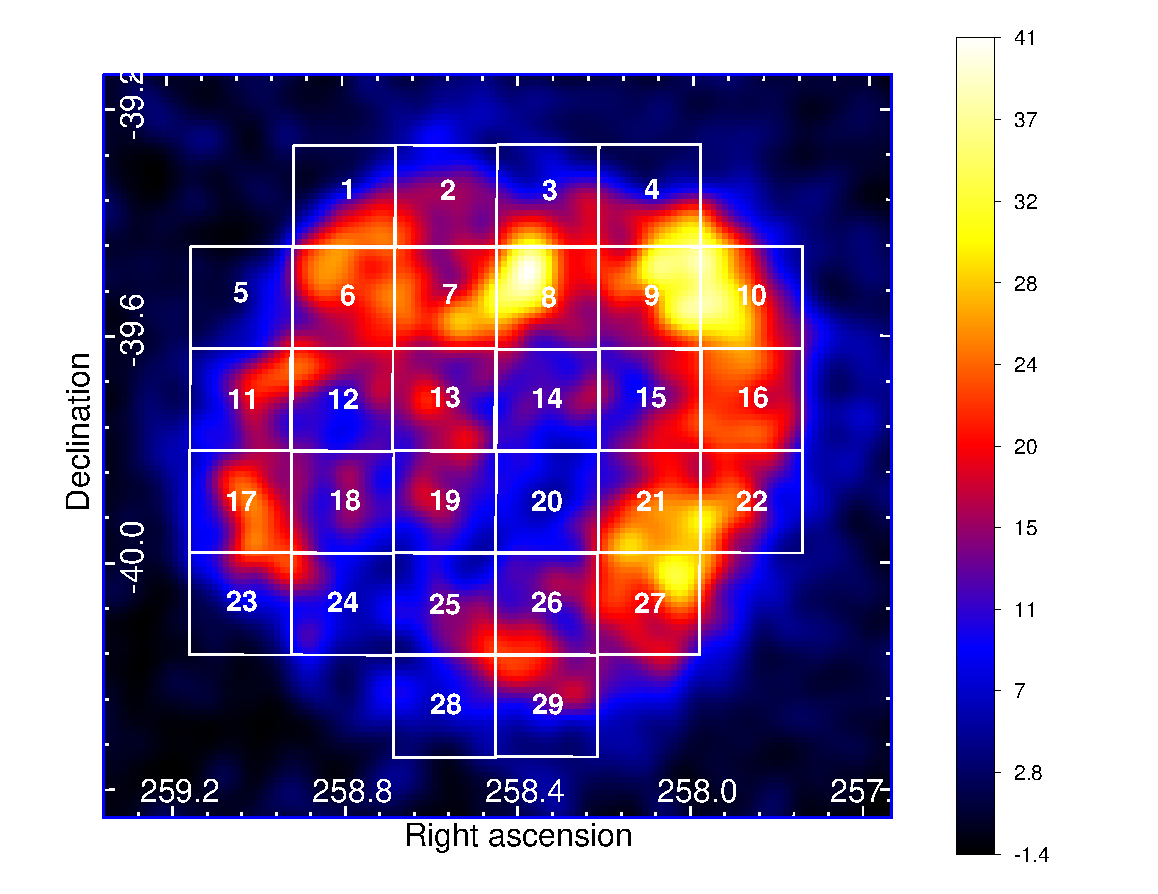
\includegraphics[width=0.7\linewidth, height=0.34\textheight]{HESS_subregions}
	\caption{HESS $\gamma$-ray image of RX J1713.7-3946 for energies greater than 2 TeV. The overlaid white squares represent the 29 sub regions.}
	\label{fig:hesssubregions}
\end{figure}
This data can be simultaneously used with \textit{Suzaku} X-ray observations, which have also been resolved to the same 29 regions \citep{2008ApJ...685..988T}, to constrain any models seeking to probe into the finer, small scale details of RX J1713.7-3946. HESS showed that these 29 sub regions can also be explained by either a pure leptonic or a pure hadronic model. Other constraints are imposed by Fermi-LAT observations at GeV-TeV $\gamma$-ray energies and ATCA radio observations \citep{2004ApJ...602..271L}. However, Fermi-LAT observations fail to resolve the fine detail needed to examine regional parts of the SNR.



The majority of studies discussed have failed to address the importance of Bremsstrahlung radiation, if any at all. One study included a Bremsstrahlung contribution in their leptonic model and found that the effects were minimal \citep{2012ApJ...751...65F} (how/why?). There are also no meaningful constraints at MeV energies where Bremsstrahlung can often be dominant, for these reasons it is often neglected.



\newpage
\section{Observations Towards RX J1713.7-3946} \label{sec:obvs}
\subsection{HESS $\gamma$-ray Observations}
This work utilizes the latest observations made by HESS across a broad range of $\gamma$-ray energies (H16). The observations are compiled from two separate viewing campaigns. The first was run from 2003-2005 and the second from 2011-2012. The first campaign involved a total of 91.3 live hours of data collection \citep{2007A&A...464..235A}. The second campaign involved a total of 78.7 live hours of data collection (H16). Figure \ref{fig:hessmap} displays the morphological image for the HESS $\gamma$-ray excess counts above the threshold energy of 2 TeV. The energy threshold was applied to increase the angular resolution from 0.048$^o$ for the entire data set to 0.036$^o$. The data were originally smoothed with a 2-dimensional Gaussian of width 0.03$^o$ and then integrated over a circle of the same radius by H16. For this work we smoothed the image again with a Gaussian of width 0.05$^o$ to ensure the contours were smooth. The contours were plotted at levels of 12.8, 26.6 and 40.5 smoothed excess counts. There is an obvious shell-like structure, characteristic of an SNR object. In section \ref{sec:corstudy} we perform gas correlations studies with this data and further investigate the shell-like features.
\begin{figure}[H]
	\centering
	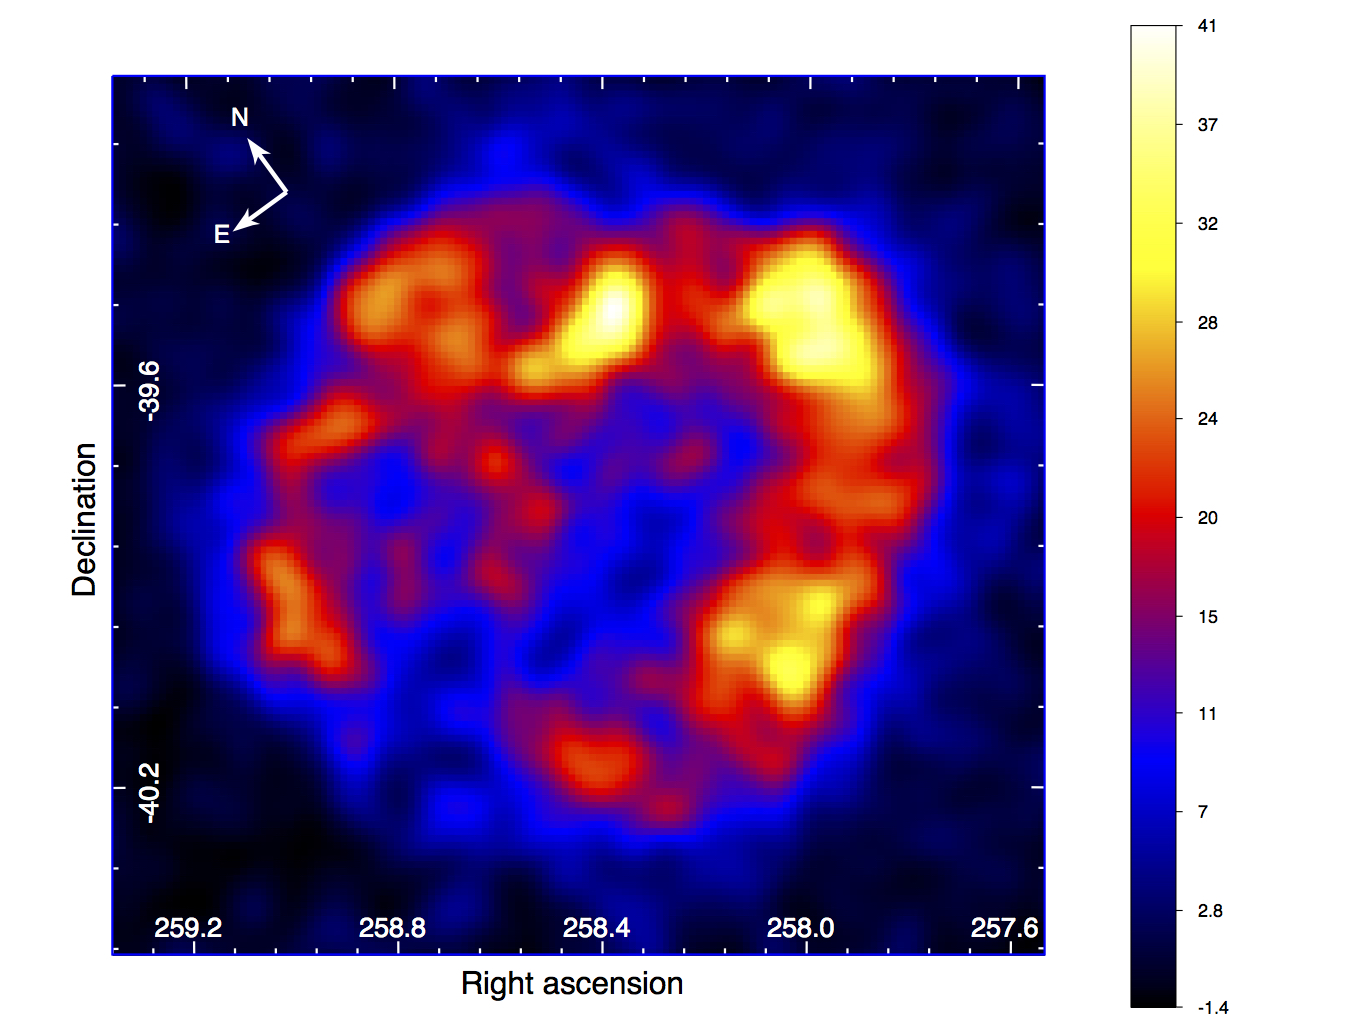
\includegraphics[width=0.74\linewidth, height=0.35\textheight]{hess_map}
	\caption{Smoothed excess counts of the HESS $\gamma$-rays above 2 TeV towards RX J1713.7-3946.}
	\label{fig:hessmap}
\end{figure}
We also obtain the latest spectral data from HESS. These data have a high resolution enabling us to break the SNR down into 29 separate regions for analysis. These data assist us with the multi-wavelength SED modeling in sections \ref{sec:seds} and \ref{sec:regseds}. 

\subsection{\textbf{\textit{Suzaku}} X-Ray Observations}
The \textit{Suzaku} X-ray observations are used for our multi-wavelength study (sections \ref{sec:seds} and \ref{sec:regseds}) but can also be applied to our morphological studies (section \ref{sec:corstudy}). \cite{2008ApJ...685..988T} provided an initial 11 pointings with this telescope and the HESS collaboration performed an additional 4 pointings in 2010 to complete the data set. The high resolution of $\mathit{Suzaku}$ enables us to resolve the spectral data into the 29 regions of interest with coverage between 1-60 keV. For an extensive outline of the data analysis method see \cite{2008ApJ...685..988T}. Figure \ref{fig:suzakumap} displays the X-ray excess counts map at 5-10 keV. There is an obvious shell-like structure much like that of the $\gamma$-ray shell. H16 performed a radial analysis towards RX J1713.7-3946 with the latest HESS $\gamma$-ray data and $\mathit{XMM-Newton}$ X-ray data and found that the radial extent of the $\gamma$-ray shell was greater than that of the X-ray shell. We observe a similar trend with the $\mathit{Suzaku}$ X-ray data here. This is interesting as it is the first time such an effect is seen in an SNR shell. H16 interpreted this finding as VHE particles escaping the main shock region, which is assumed to be located at the peak of the shell emission, and producing $\gamma$-rays outside the shock region. 
\begin{figure}[H]
	\centering
	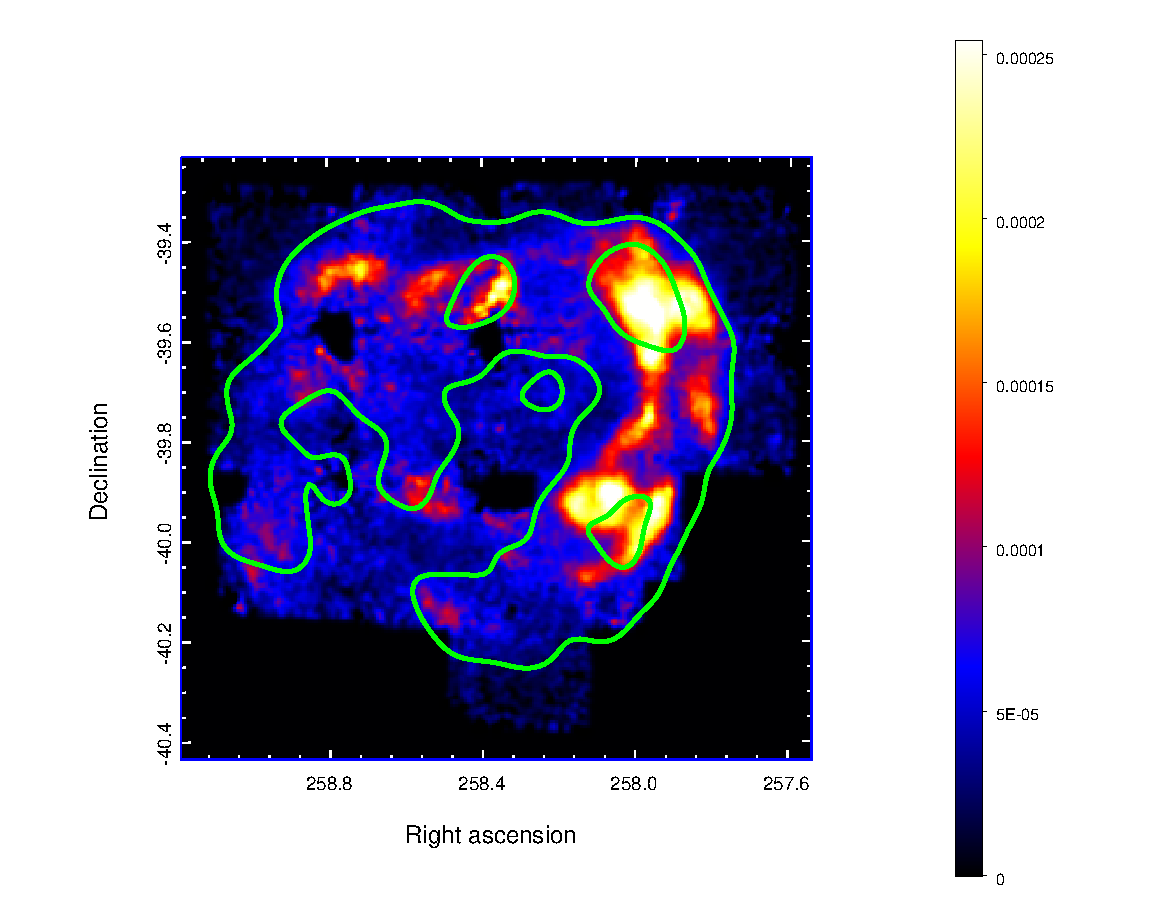
\includegraphics[width=0.75\linewidth, height=0.36\textheight]{suzaku_map}
	\caption{$\mathit{Suzaku}$ X-ray image towards RX J1713.7-3946 at 5-10 keV with the HESS ($>2$ TeV) contours overlaid in green.}
	\label{fig:suzakumap}
\end{figure}

\subsection{Fermi-LAT Observations}
We use the latest Fermi-LAT observations of RX J1713.7-3946 in our multi-wavelength SED study \citep{2011ApJ...734...28A}. The Fermi-LAT data cover an energy range from 200 MeV to 300 GeV. Unfortunately the Fermi-LAT data is not resolvable enough to examine the smaller 29 regions of interest. However, we still use the data for the whole remnant as an upper limit when modeling our SEDs. 

\subsection{Gas and Radio Observations}
\subsubsection{ATCA}
Observations in the radio spectrum assist with multi-wavelength SED modeling of $\gamma$-rays as radio emission is an indicator for the production of Synchrotron radiation. We obtained the spectral data observed by ATCA at 1.4 and 2.5 GHz ($\approx$ 6 and 10 $\mu$eV respectively) from  \cite{2004ApJ...602..271L}. We also used the high resolution 1.4 GHz image to obtain spectral data for each of our 29 smaller regions. Figure \ref{fig:atcaradiomap} displays the radio image, in units of Jansky/beam, overlaid with the HESS contours and the 29 regions of interest. Again we observed shell-like features, this time in the form of arcs along the eastern side of the source. The radio flux for each region can be obtained with DS9 but requires a conversion to cgs units (equation \ref{eq:Jytocgs}).
\begin{equation} \label{eq:Jytocgs}
\begin{split}
1 \ \mathrm{Jy} &= 1 \times 10^{-23} \, \mathrm{erg \, s}^{-1} \ \mathrm{cm}^{-2} \ \mathrm{Hz}^{-1} \\
1  \ \mathrm{Jy\, beam}^{-1} &= \dfrac{\nu_o \times 10^{-23}}{P}  \ \mathrm{erg \, s}^{-1} \ \mathrm{cm}^{-2}
\end{split}
\end{equation}
where P is the number of pixels within a beam area and $\nu_o$ is the frequency at which the observations were made. The beam size is $4.0589 \times 10^{-4}$ squared degrees \citep{2004ApJ...602..271L}, whilst the area of a pixel is $4.406 \times 10^{-6}$ squared degrees, hence 92 pixels fit within 1 beam. The observed flux for each region is presented in table \ref{tab:atcaobvs}.
\begin{figure}[H]
	\centering
	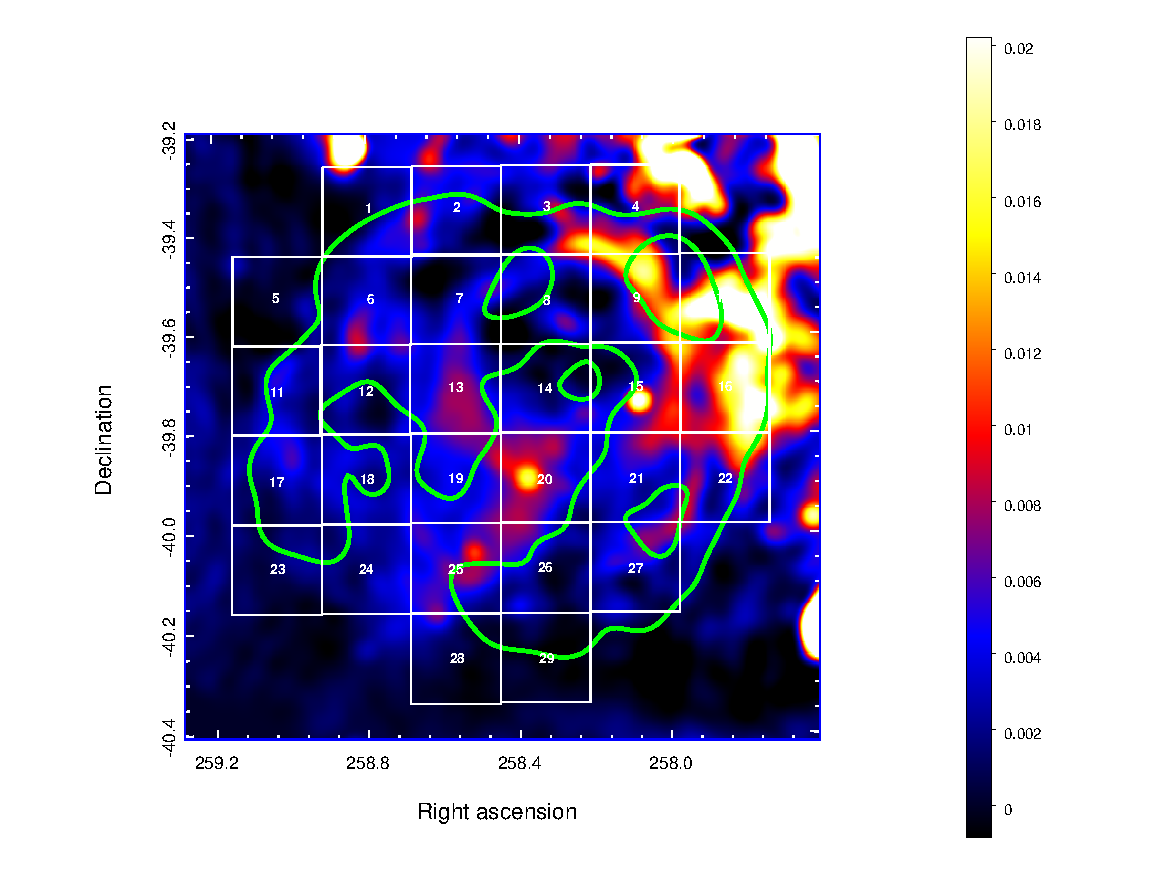
\includegraphics[width=0.75\linewidth, height=0.35\textheight]{atca_map}
	\caption{ATCA radio image towards RX J1713.7-3946 overlaid with the HESS $\gamma$-ray ($>2$TeV) contours the 29 sub-regions.}
	\label{fig:atcaradiomap}
\end{figure}
\begin{table}[H] 
	\begin{center}
		\begin{tabular}{cccccc}
			\toprule
			Reg. & Flux (erg s$^{-1}$ cm$^{-2}$) & Reg. & Flux (erg s$^{-1}$ cm$^{-2}$) & Reg. & Flux (erg s$^{-1}$ cm$^{-2}$) \\ 	
			& $\times 10^{-15}$ && $\times 10^{-15}$ && $\times 10^{-15}$ \\
			\hline 
			1& 2.31  & 11 & 2.16  & 21 & 4.55   \\ 
			2& 3.81   & 12 & 2.84  & 22 & 7.03   \\ 
			3& 3.89  & 13 & 5.69  & 23 & 1.14  \\ 
			4& 9.45  & 14 & 2.29  & 24 & 2.52  \\ 
			5& 0.33   & 15 & 6.07 & 25 & 5.84   \\ 
			6& 3.47   & 16 & 14.86  & 26 & 2.76   \\ 
			7& 2.20  & 17 & 2.68  & 27 & 3.52   \\ 
			8& 2.26   & 18 & 3.21  & 28 & 7.90   \\ 
			9& 8.56   & 19 & 5.13  & 29 & 1.43   \\ 
			10& 18.37   & 20 & 7.06  && \\ 
			\bottomrule
		\end{tabular} 
	\end{center}
	\caption{The observed radio flux at 1.4 GHz for each region within RX J1713.7-3946.}
	\label{tab:atcaobvs}
\end{table}

\subsubsection{The Southern Galactic Plane Survey}
The Southern Galactic Plane Survey (SGPS) combines data from the ATCA (mentioned above) and Parkes Radio Telecope. The Parkes survey was responsible for the low resolution data, while the ATCA survey was responsible for the high resolution data. The SGPS data were taken at a wavelength of 21 cm (1.4 GHz) i.e. the HI spectral line. Hence, this data is used to represent the flux or brightness temperature of HI gas. The image towards RX J1713.7-3946 is obtained from \cite{2005ApJS..158..178M} and is presented in figure \ref{fig:SGPSmap}. The units of brightness temperature have already been converted to that of column density (cm$^{-2}$) according to equation \ref{eq:HIcoldens}.
\begin{equation}
\label{eq:HIcoldens}
N_{HI} = 1.823 \times 10^{18} \int T(v) dv \ \mathrm{ cm}^{-2}
\end{equation} 
where $T$ is the brightness temperature and $v$ is the velocity. The data were integrated from -20 km/s to 0 km/s with a velocity resolution and rms noise fluctuations of $\Delta v = 0.82$ km/s and $T_{rms} = 1.6$ K, respectively. The angular resolution of the survey is approximately 2.2$^\prime$. The shell-like features of the HI gas stand out around the south-west, north and east regions of the source. We interpret this as the shock front accelerating the HI gas into clumps around the shell. Much of the gas is also contained within the $\gamma$-ray shell. This could be an indication that the gas is located in the foreground of the spherical SNR shell. These data are used to assist in the latest ISM gas density calculations (section \ref{sec:seds} and \ref{sec:regseds}) and also for gas correlations studies (section \ref{sec:corstudy}).
\begin{figure}[H]
	\centering
	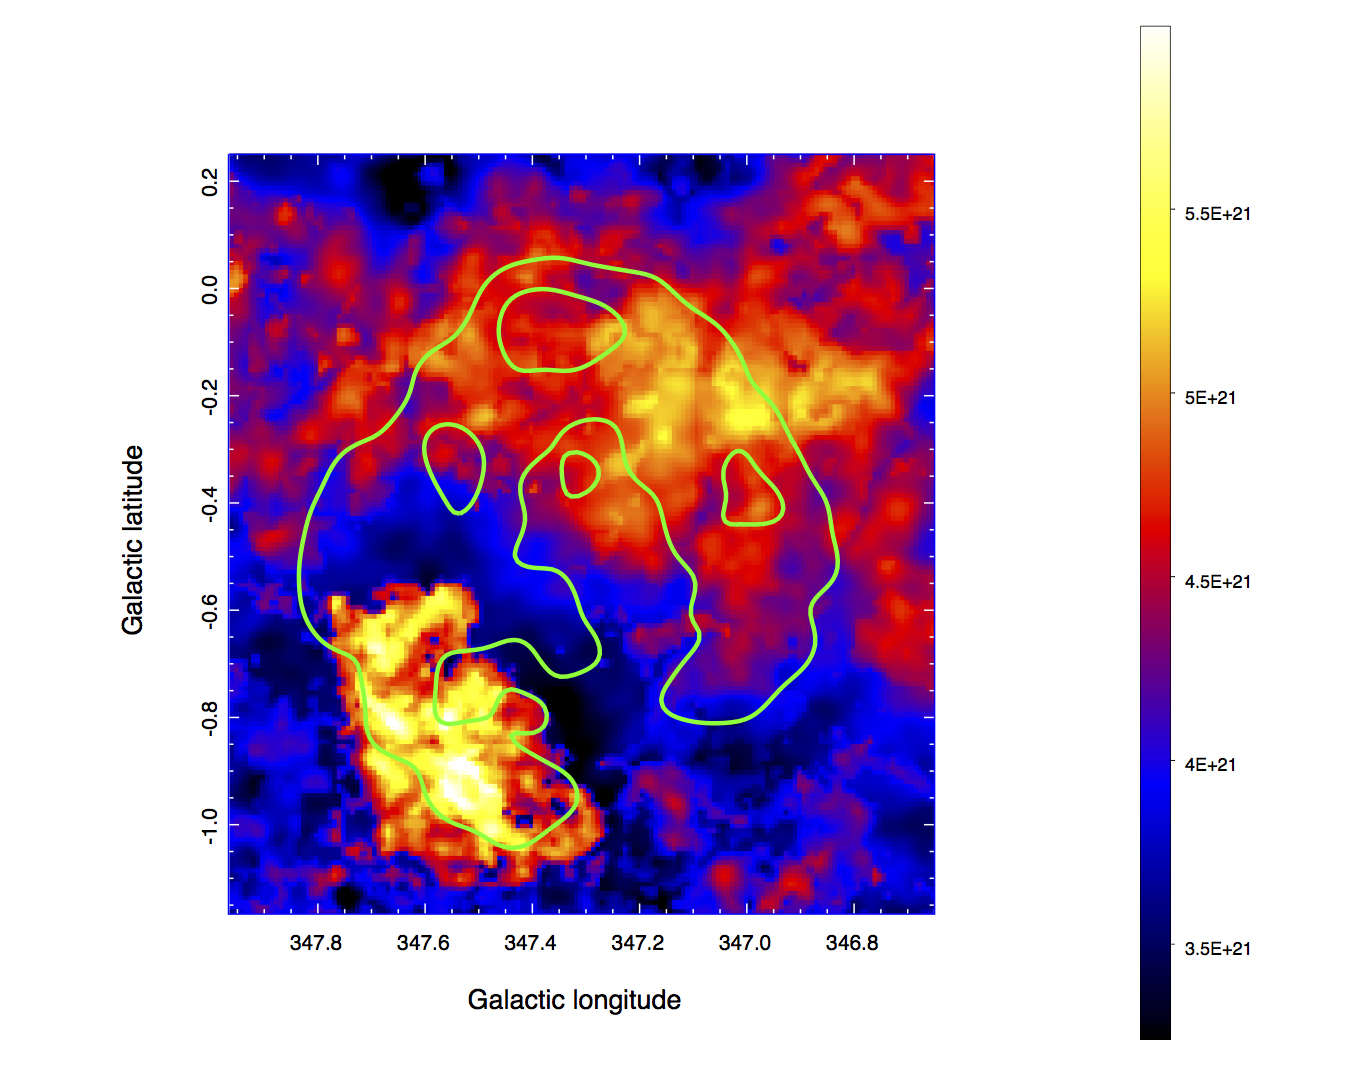
\includegraphics[width=0.75\linewidth, height=0.36\textheight]{SGPS_HI_map}
	\caption{SGPS survey }
	\label{fig:SGPSmap}
\end{figure}
\subsubsection{Mopra}
In addition to the atomic hydrogen, HI, we can also estimate the column density of molecular hydrogen, H$_2$, through its tracer $^{12}$CO. We obtain the Mopra $^{12}$CO image from \cite{2013PASA...30...44B}. Again the data were integrated from -20 km/s to 0 km/s with a velocity resolution and rms noise fluctuations of $\Delta v = 0.11$ km/s and $T_{rms} = 0.7$ K, respectively. The units of intensity are brightness temperature (K km/s). The image we received was re-binned from the original pixel size of 0.5$^\prime$ to 5$^{\prime}$. Figure \ref{fig:mopramap} presents the Mopra image overlaid with the green HESS TeV contours. The Mopra contours are also overlaid in white at levels of 5, 25 and 40 K km/s. These levels are chosen to emphasize the peaks and also the ring structure surrounding the dim gas/cavity. There are regions of bright gas around the north section of the source and also down to the east. These regions follow a shell-like structure much like the $\gamma$-ray contours. The white arrow points towards a region of peak brightness still contained within the shell. It could be that this feature is again located on the foreground of the SNR shell. These data also assist in gas correlation studies in section \ref{sec:corstudy}.
\begin{figure}[H]
	\centering
	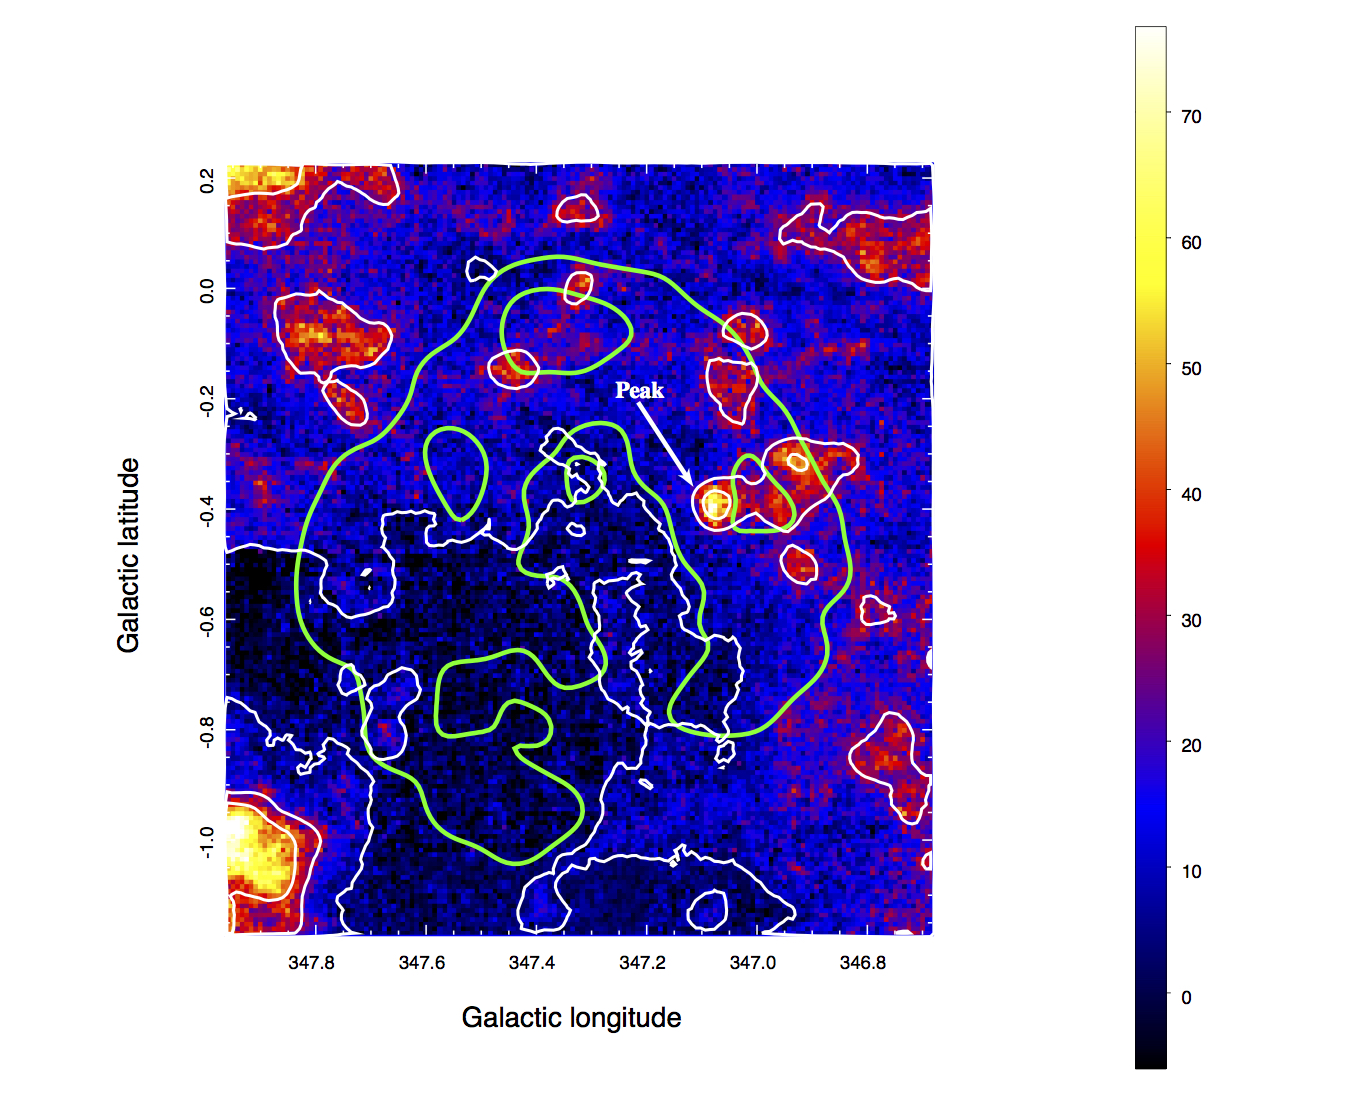
\includegraphics[width=0.73\linewidth, height=0.35\textheight]{mopra_map}
	\caption{Mopra map}
	\label{fig:mopramap}
\end{figure}
\subsubsection{Nanten}
In the same way that the Mopra data are used as a tracer for molecular hydrogen, Nanten $^{12}$CO data are also. We expect the two data sets to be very similar, however the resolution of Nanten is lesser than that of Mopra. The Nanten data were obtained from \cite{2012ApJ...746...82F} but have also been used by \cite{2005ApJ...631..947M} in the past. The data were integrated from -20 km/s to 0 km/s with a velocity resolution and rms noise fluctuations of $\Delta v = 0.65$ km/s and $T_{rms} = 0.3$ K, respectively. The beam size of the telescope was 2.6$^\prime$. Figure \ref{fig:nantenmap} presents the Nanten image with the Mopra contours overlaid in white. The Mopra contours can be seen to overlap almost perfectly with the Nanten image as expected. However we can see regions where the Nanten telescope fails to resolve some of the low density gas. This is evident north of the contours around the cavity, where there are more dark regions. The gas here has a brightness temperature close to 0, when compared to Mopra it should be slightly more than this ($\sim 10$). A more thorough correlation study between the two data sets is included in the appendix. We use these data in section \ref{sec:corstudy} for our gas correlation study and also to calculate the gas density in each of our regions of interest (section \ref{sec:regseds}).
\begin{figure}[H]
	\centering
	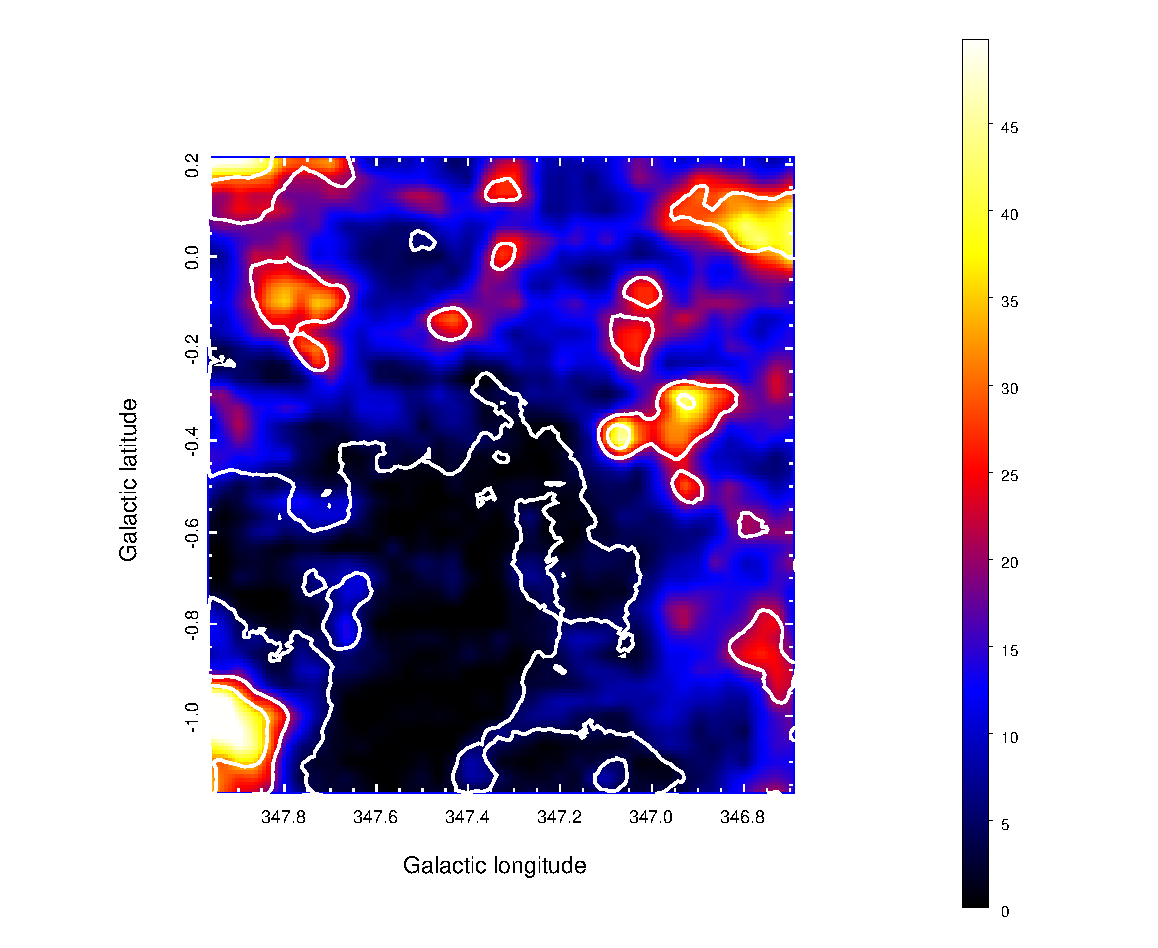
\includegraphics[width=0.73\linewidth, height=0.35\textheight]{nanten_map}
	\caption{Nanten $^{12}$CO image towards RX J1713.7-3946 integrated over the velocity range -20-0 km/s and overlaid with the white Mopra contours.}
	\label{fig:nantenmap}
\end{figure}


\newpage
\section{SED Modeling of RX J1713.7-3946 - Whole SNR Region} \label{sec:seds}


The SED code sedprodv2.c has been verified for other sources (see appendix) and can be applied to the source of interest for this research project, RX J1713.7-3946. The HESS collaboration investigated both the hadronic and leptonic origins of $\gamma$-rays from this source (H16), providing another framework to compare against and to expand on. 

\subsection{Particle Distributions}
The electron and proton distributions were simulated using a power law with a cut off (equation \ref{eq:4}), using the parameters in table \ref{tab:paramshess} (table 5 in H16).
\begin{table}[H] 
	\begin{center}
		\begin{tabular}{ccc}
			\toprule
			Parameters & Proton & Electron \\ 
			\hline 
			$\alpha$& 1.53 & 1.78 \\ 
			$\beta$& 1.94 & 2.93 \\ 
			$E_{b}$ (TeV)& 1.4 & 2.5 \\ 
			$E_{c}$ (TeV)& 93 & 88.5 \\ 
			$B$ ($\mu$G) & - & 12\\
			\bottomrule
		\end{tabular} 
	\end{center}
	\caption{HESS proton and electron distribution parameters}
	\label{tab:paramshess}
\end{table}
The injection energy for the proton population, with an ISM gas cloud density of $n_H$, is specified as $W_p(>1 $TeV$) = 5.80 \times 10^{49}(1 $cm$^{-3}/n_H)$ erg. While the electron population only requires an injection energy of $W_e(>1 $TeV$) = 1.19 \times 10^{47}$ erg. \cite{2012ApJ...746...82F} take the average density of protons over the entire SNR region to be $n_H = 130$ cm$^{-3}$. It should be noted that the injection energy of the parent populations was specified only above 1 TeV in H16. A code was written to renormalise these values to an injection energy for the whole energy spectrum, as required by sedv2.c. The normalisation simply follows the following idea of rearranging for the normalisation constant A in equation \ref{eq:injenergy},
\begin{equation*}
\begin{split}
W\mathrm{(>1TeV)} = A\int_{1 \mathrm{TeV}}^{\infty}  E^{-\alpha + 1} dE\\
A = \dfrac{W\mathrm{(>1TeV)}}{\int_{1 \mathrm{TeV}}^{\infty}  E^{-\alpha + 1} dE}.\\
\end{split}
\end{equation*}
Hence the total particle injection energy is
\begin{equation} \label{eq:renormal}
\begin{split}
W = A\int_{\mathrm{E_0}}^{\infty}  E^{-\alpha + 1} dE\\
W = \dfrac{W\mathrm{(>1TeV)}}{\int_{1 \mathrm{TeV}}^{\infty}  E^{-\alpha + 1} dE}\int_{\mathrm{E_0}}^{\infty}  E^{-\alpha + 1} dE\\
\end{split}
\end{equation}
where E$_0$ is the rest mass energy for the appropriate particle. This was done assuming a simple power law, but it is easily adapted for any of the other functional forms. For our model, a conversion of the injection energies above 1 TeV results in a total injection energy of $W_p = 6.55 \times 10^{47}$ erg and $W_e  = 5.22 \times 10^{47}$ erg. \\

A comparison of our parent particle distributions is made with those of HESS. As can be seen in Figure \ref{fig:rxj1713spectrumboth}, both particle distributions agree with the HESS models, aside from a slight discrepancy in the electron spectrum between 2.5-10 TeV. This confirms the correctness of the code when dealing with impulsive scenarios (SNRs) at the particle distribution level.
\begin{figure}[H]
	\centering
	\includegraphics[width=0.52\linewidth, height=0.4\textheight, angle=-90]{rxj1713_spectrum_both.ps}
	\caption{Proton and electron distributions compared with the HESS model.}
	\label{fig:rxj1713spectrumboth}
\end{figure}

The $\gamma$-ray emission is then modeled assuming that the source is impulsive and evolves with time. Using the favoured distance of 1 kpc, our source has a radius of 10.5 pc. An age of 150 years, the time since the CRs were ejected, was found by matching our particle distribution models to those of HESS (figure \ref{fig:rxj1713spectrumboth}). 


\subsection{Leptonic Model}
The IC model was calculated using the CMB ($T = 2.7$ K and $U_{rad} = 0.26$ eV cm$^{-3}$) and a far-infrared photon field ($T = 26.5$ K and $U_{rad} = 0.415$ eV cm$^{-3}$). The model was fitted to the HESS and Fermi-Lat spectrum for the whole SNR by using the electron distribution parameters from table \ref{tab:paramshess}. The synchrotron model was fitted to the \textit{Suzaku} and ATCA observations, assuming the same population of electrons and by altering the magnetic field until the model was normalised correctly against the IC model. The magnetic field was found to be $B = 14.26 \ \mu$G. Lastly, the Bremsstrahlung model was computed with a target gas density of $n_H = 130$ cm$^{-3}$, this model was not fitted to any observations. It was included to determine whether its contribution is comparable to the IC contribution\\

Figure \ref{fig:rxj1713lep} displays the leptonic model including the comparison with the HESS models and also includes the Bremsstrahlung contribution, which HESS did not. The Bremsstrahlung contribution is less than 1 order of magnitude smaller than the IC peak at TeV energies. There appears to be some discrepency between our model and the HESS model. In terms of the actual data points at TeV energies, the Bremsstrahlung component is only a factor 3 to 4 smaller. Bremsstrahlung is also dominant around the MeV range, where unfortunately, observational data are not available as Fermi-LAT observations aren't easily resolvable at these energies. The latest ISM gas density measurements have given us an indication that the Bremsstrahlung component is quite significant around this source. This shows that Bremsstrahlung shouldn't necessarily be neglected, especially for a source with surrounding dense ISM gas. The gas density isn't constant for the whole source however, here we have applied an average density over the whole region. A sub-regional analysis with more accurate density values is applied in the next chapter. 
\begin{figure}[H]
	\centering
	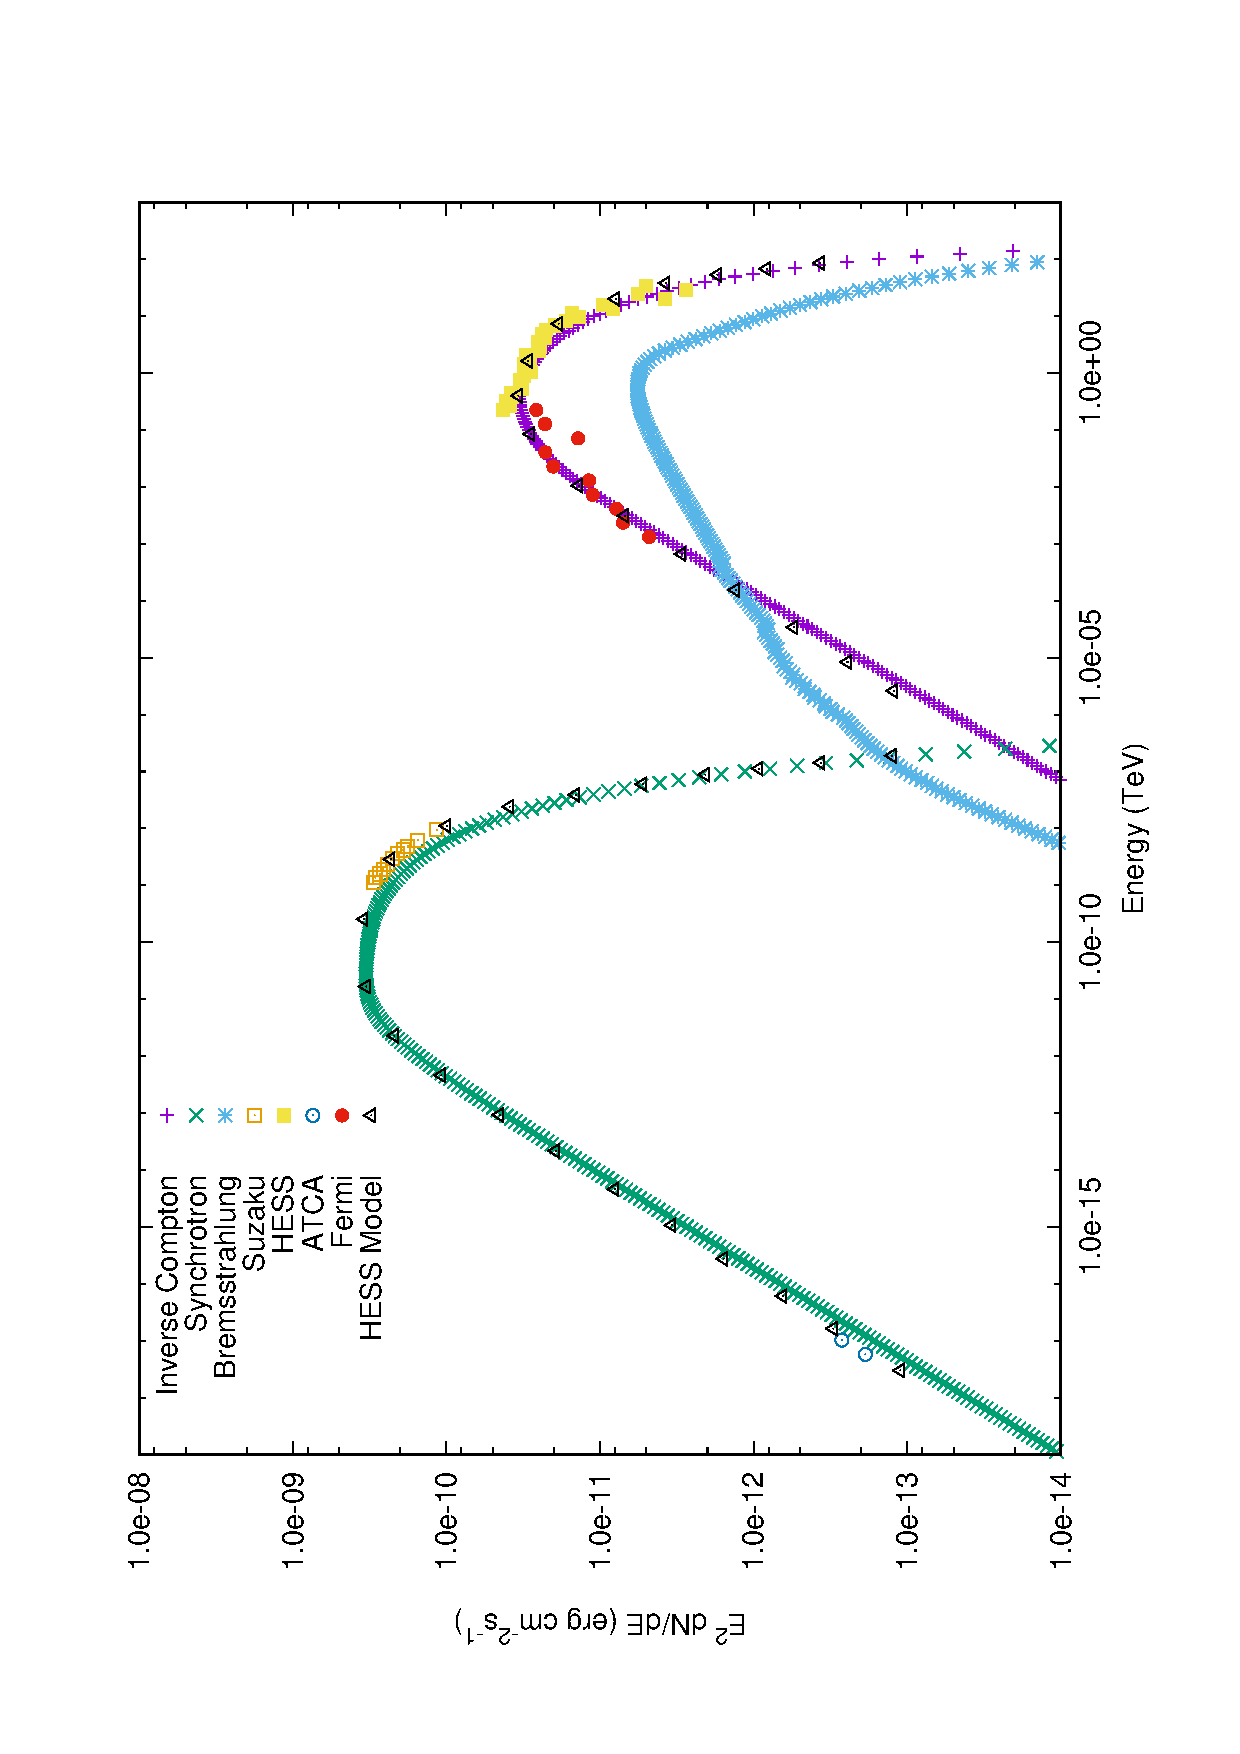
\includegraphics[width=0.45\linewidth, height=0.35\textheight, angle=-90]{rxj1713_lep}
	\caption{SED of the Leptonic model of $\gamma$-ray flux for source RX J1713.7-3946.}
	\label{fig:rxj1713lep}
\end{figure}

\subsection{Hadronic Model}
The hadronic model was calculated with the latest ISM gas density value for the SNR ($n_H = 130$ cm$^{-3}$) and the proton distribution parameters from table \ref{tab:paramshess}. The model was fitted to both the HESS and Fermi-LAT observations. 

Figure \ref{fig:rxj1713had} displays the hadronic model including the comparison with the HESS model and the HESS and Fermi-LAT data. The model fitted with Fabien's code has a slight discrepancy with regards to the total flux output, regardless, both models seem consistent with each other and the observations. The hadronic model does however fail to explain the radio and X-ray data, this is a common reason for favouring a leptonic model or pushing for a combined model. 
\begin{figure}[H]
	\centering
	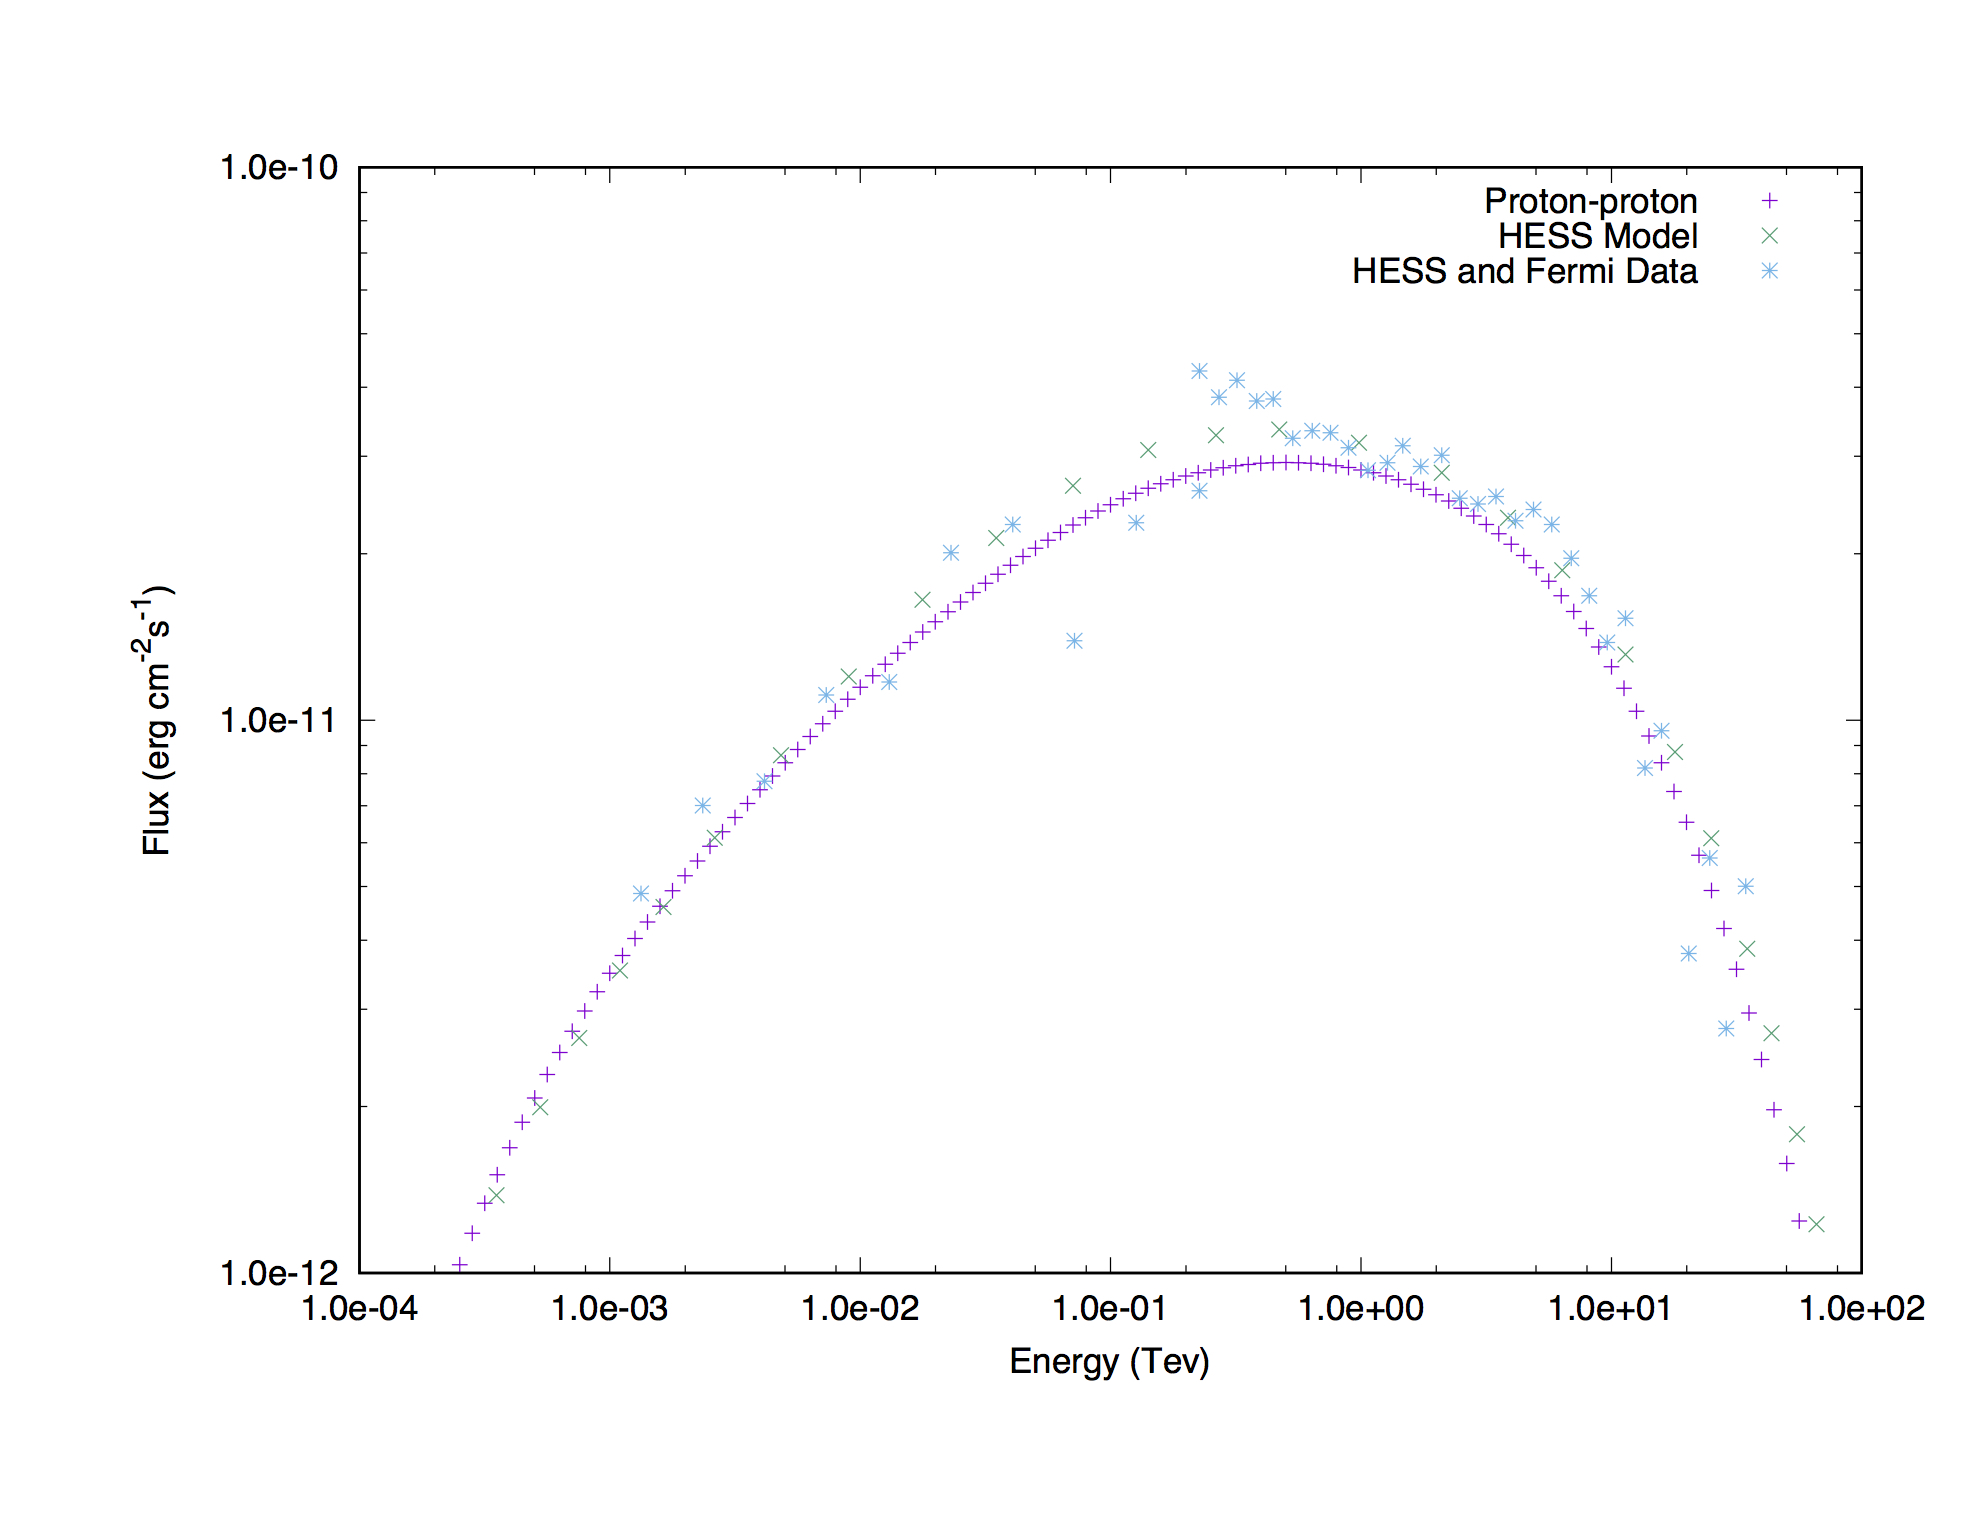
\includegraphics[width=0.45\linewidth, height=0.35\textheight, angle=-90]{rxj1713_had}
	\caption{SED of the Hadronic model of $\gamma$-ray flux for source RX J1713.7-3946.}
	\label{fig:rxj1713had}
\end{figure}
One factor that does favour a hadronic model is the presence of gas around the source. If there is gas present then the CR protons ejected from the SNR could undergo PP interactions with the gas, contributing to the $\gamma$-ray flux. A correlation study will help us better understand this effect. Figure \ref{fig:mopramap} illustrates the latest Mopra $^{12}$CO gas density map of RX J1713.7-3946 overlaid with the HESS $\gamma$-ray contours (green) taken from figure \ref{fig:hessmap}. There appears to be a correlation between the gas and the $\gamma$-rays in the north and north-east region of the source. This is a good indication of hadronic processes being present in these regions. Again, because RX J1713.7-3946 is such a big source it makes sense to investigate the hadronic nature of the sub-regions. This is the focus of the chapter \ref{sec:regseds}. We then analyse the gas data more closely in chapter \ref{sec:corstudy} .


\subsection{Combined Model}
A combined hadronic/leptonic model of the entire SNR source is presented in this section. To fit the combined model to the data we began with the HESS parameters from table \ref{tab:paramshess}. We also chose a proton fraction of 0.99 to begin with, leaving it and the magnetic field strength as a free parameter. Extremely high magnetic fields were required to provide the synchrotron emission observed with a proton fraction this high. Not until the proton fraction is lowered to 0.60 is a suitable magnetic field obtained ($B =$ 25.3 $\mu$G). The particle distribution parameters were also altered in order to make a better fit, see table \ref{tab:paramscomb}. Figure \ref{fig:rxj1713comb} displays the final combined model (purple addition signs) including all the individual contributions. A combined model can be used to explain the observed spectrum of RX J1713.7-3946, with a low proton fraction and a large magnetic field. It is unlikely that the fraction of protons would drop this much for a source as close as RX J1713.7-3946. There is also little understanding of the small scale turbulent magnetic fields within SNRs, so a magnetic field value of 25.3 $\mu$G may not be completely unphysical. We now move to investigate the sub-regions of RX J1713.7-3946.
 \begin{table}[H] 
 	\begin{center}
 		\begin{tabular}{ccc}
 			\toprule
 			Parameters & Proton & Electron \\ 
 			\hline 
 			$\alpha$& 1.30 & 1.82 \\ 
 			$\beta$& 1.94 & 2.93 \\ 
 			$E_{b}$ (TeV)& 1.4 & 2.5 \\ 
 			$E_{c}$ (TeV)& 93 & 110 \\ 
 			\bottomrule
 		\end{tabular} 
 	\end{center}
 	\caption{Combined model proton and electron distribution parameters}
 	\label{tab:paramscomb}
 \end{table}
\begin{figure}[H]
	\centering
	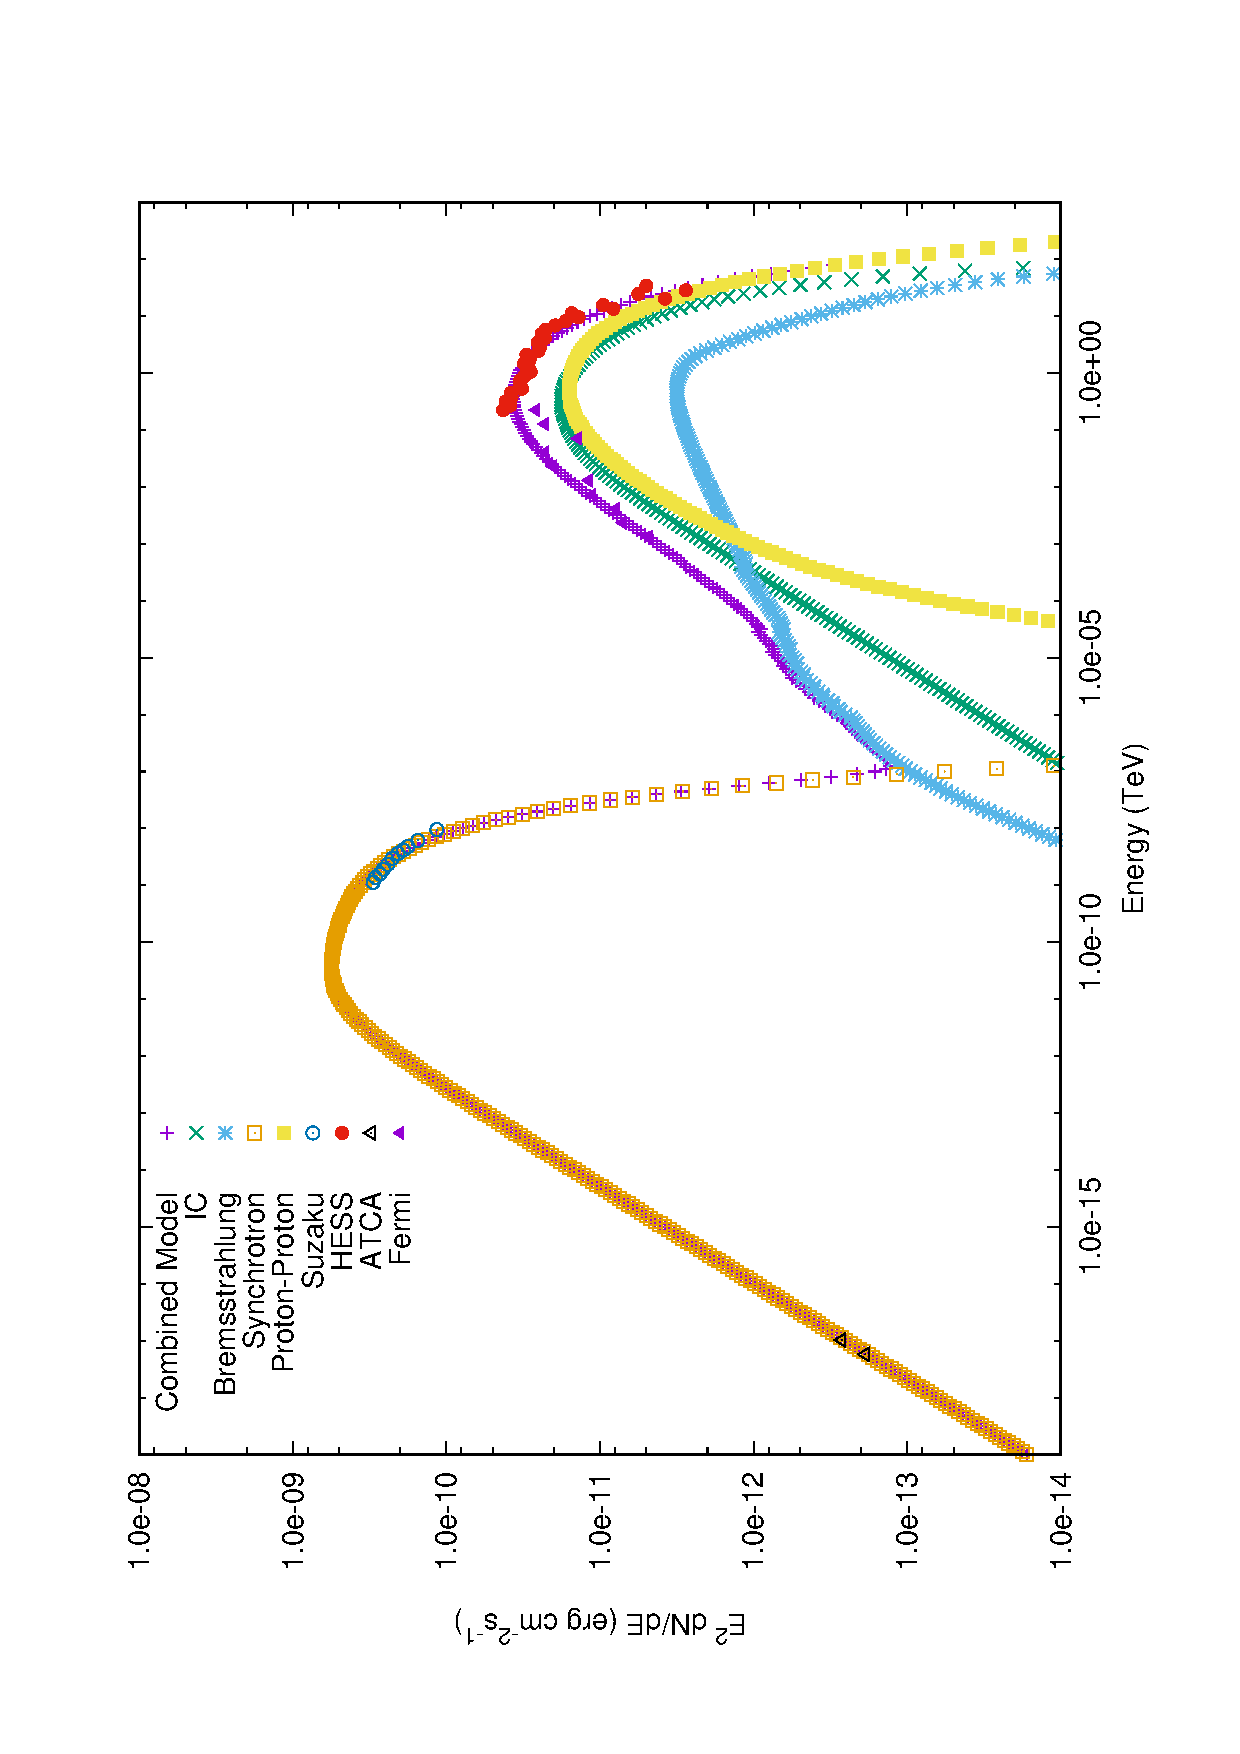
\includegraphics[width=0.45\linewidth, height=0.35\textheight, angle=-90]{rxj1713_comb}
	\caption{}
	\label{fig:rxj1713comb}
\end{figure}


\newpage
\section{Regional SED Modeling Towards RX J1713.7-3946} \label{sec:regseds}
As mentioned earlier, the work by HESS also investigated 29 smaller regions, originally proposed by \cite{2008ApJ...685..988T} when they examined the \textit{Suzaku} X-ray data. We attempted to model these regions with both a pure hadronic and pure leptonic model separately. In doing so we hoped to reveal the success of each scenario in predicting the observations. We also examined the significance, if any, of Bremsstrahlung within each of the regions and whether or not this should be neglected as a source of $\gamma$-rays. Combined models of the regions were also investigated to help determine the nature of the parent particles. As defined in \cite{2008ApJ...685..988T}, each square region has a size of 10.8$^\prime$ x 10.8$^\prime$ = 0.18$^o$ x 0.18$^o$, which corresponds to a width and height of approximately 3.2 pc. This value will was assumed throughout the work for any analysis involving the regions, unless specified.


\subsection{Regional ISM Gas Density Calculations} \label{sec:regdenscalc}
\cite{2012ApJ...746...82F} perform an analysis on the SGPS HI gas data and the NANTEN $^{12}$CO data to calculate the observed ISM gas density, $n_H$, towards RX J1713.7-3946 for the entire SNR source. We performed a similar analysis to obtain the ISM gas density for our 29 regions of interest. This is an important parameter for modeling PP interactions and Bremsstrahlung processes. The ISM gas density was modeled as the total number of protons. The total number of protons in a given region, or proton column density, $N_H$, was obtained by summing the H$_2$ and HI components. The H$_2$ component was derived from the NANTEN $^{12}$CO gas map, while The HI gas map was taken from the SGPS at 21 cm (see section \ref{sec:obvs}). We used a velocity range of -20 to 0 km s$^{-1}$. The HI map is already in units of column density, however we applied an X factor to the NANTEN data to convert it from brightness temperature (equation \ref{}). In being consistent with \cite{2012ApJ...746...82F} we adopted an X factor of $2.0 \times 10^{20}$. We then multiplied the H$_2$ column density by a factor of 2 to convert it into a proton column density and combined it with the HI column density map. We split the total proton column density map into our 29 regions for analysis in DS9 (figure \ref{fig:rxj1713Nproton}). To obtain the proton density, n$_H$, for each region the proton column density was divided by the approximate depth of the SNR in that region. We assumed the SNR to be spherical to take the depth in the centre of the SNR to be similar to that of the width at the widest point (6 regions plus some). Regions in the middle were taken to have a depth of about 22.4 pc, which corresponds to a depth of 7 regions. Regions on the rim of the SNR were taken to have a depth of 12.8 pc, corresponding to a depth of 4 regions. The remaining regions were taken to have a depth somewhere within these two extremities. The density for each region can be found in table \ref{tab:regionalparams}.
\begin{figure}[H]
	\centering
	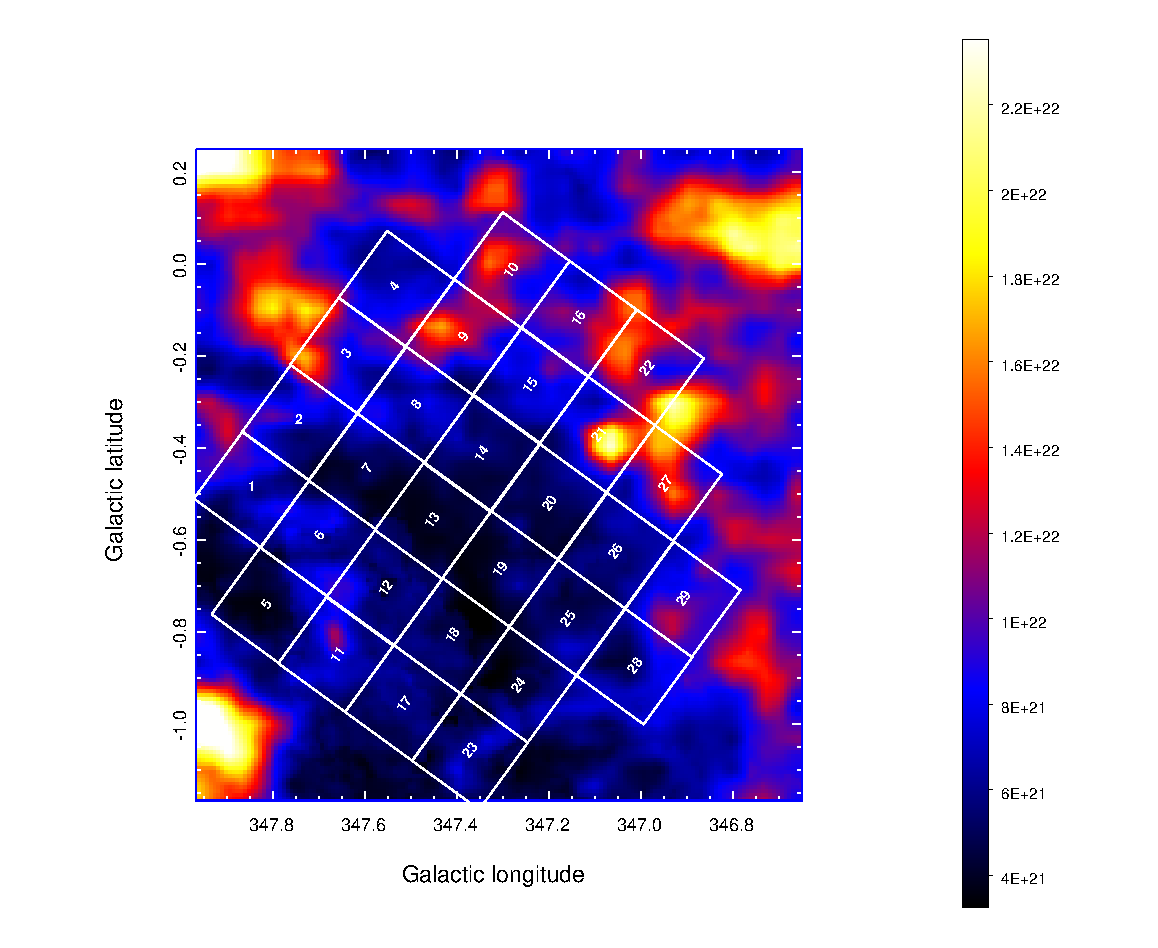
\includegraphics[width=0.8\linewidth, height=0.4\textheight]{sgps+nanten_regmap}
	\caption{The total proton column density map using the combined SGPS and NANTEN contributions overlaid with the 29 regions of interest.}
	\label{fig:rxj1713Nproton}
\end{figure}
\begin{table}[H] 
	\begin{center}
		\begin{tabular}{cccccccc}
			\toprule
			Reg. & n$_H$ (cm$^{-3}$) && Reg. & n$_H$ (cm$^{-3}$) && Reg. & n$_H$ (cm$^{-3}$) \\ 
			\hline 
			1& 105 && 11 & 102  && 21 & 159   \\ 
			2& 107 && 12 & 86  && 22 & 181   \\ 
			3& 143 && 13 & 72  && 23 & 79  \\ 
			4& 112 && 14 & 88  && 24 & 72  \\ 
			5& 70 && 15 & 110 && 25 & 78   \\ 
			6& 97 && 16 & 152  && 26 & 86   \\ 
			7& 70 && 17 & 79  && 27 & 162   \\ 
			8& 102 && 18 & 68  && 28 & 98   \\ 
			9& 152 && 19 & 65  && 29 & 133   \\ 
			10& 156 && 20 & 74  && & \\ 
			\bottomrule
		\end{tabular} 
	\end{center}
	\caption{The calculated proton density for each region towards RX J1713.7-3946.}
	\label{tab:atcaobvs}
\end{table}



\subsection{Hadronic Model} 
In this section we investigate the role of the hadronic production scenario in each region. We begin by outlining the SED modeling process and then proceed to present the results. We then examine the accuracy of our SED modeled injection energies, $W_{p,\mathrm{SED}}$, for each region, by comparing against two different theoretical predictions. 

\subsubsection{SED Model}
The hadronic spectra for each region were modeled using the latest ISM gas density measurements, $n_H$. A power law with a cut-off was used and the particle index $\alpha$ was taken from H16. A cut-off energy of $93$ TeV was used for all regions (H16). To fit the models, the injection energy's, $W_{p,\mathrm{SED}}$, were adjusted to fit the HESS data points, while the global Fermi-LAT data (e.g. data for the entire SNR region) were used as an upper limit. To check whether these values conformed to those predicted by H16 ($W_p\mathrm{(>1TeV)}$($n_H$/1cm$^{-3}$)$^{-1}$ erg), we normalised $W_{p,\mathrm{SED}}$ to energies above 1 TeV and divided by $n_H$ (equation \ref{eq:normdens}).
\begin{equation}\label{eq:normdens}
W_{p,\mathrm{SED}}\mathrm{(>1TeV)} (n_H/1 \ \mathrm{cm}^{-3})^{-1} \ \mathrm{erg} = \dfrac{1}{n_H}\dfrac{W_{p,\mathrm{SED}}}{\int_{\mathrm{E_0}}^{\infty}  E^{-\alpha + 1} dE}\int_{1 \mathrm{TeV}}^{\infty}  E^{-\alpha + 1} dE\\
\end{equation}
The models generally fitted the HESS data comfortably (figure \ref{fig:regionalhadseds} illustrates 6 such regions) and our $W_{p,\mathrm{SED}}$ values conformed to those in H16. The specta for regions 15 and 22 were hard at low energies, almost reaching the upper limit imposed by the global Fermi-LAT observations. The spectra of regions 16 and 21 approached this limit also. For comparison, these 4 spectra were displayed with spectra that don't appear to be violating this limit (regions 5 and 24). 
\begin{figure}[H]
	\begin{subfigure}{0.5\textwidth}
		\centering
		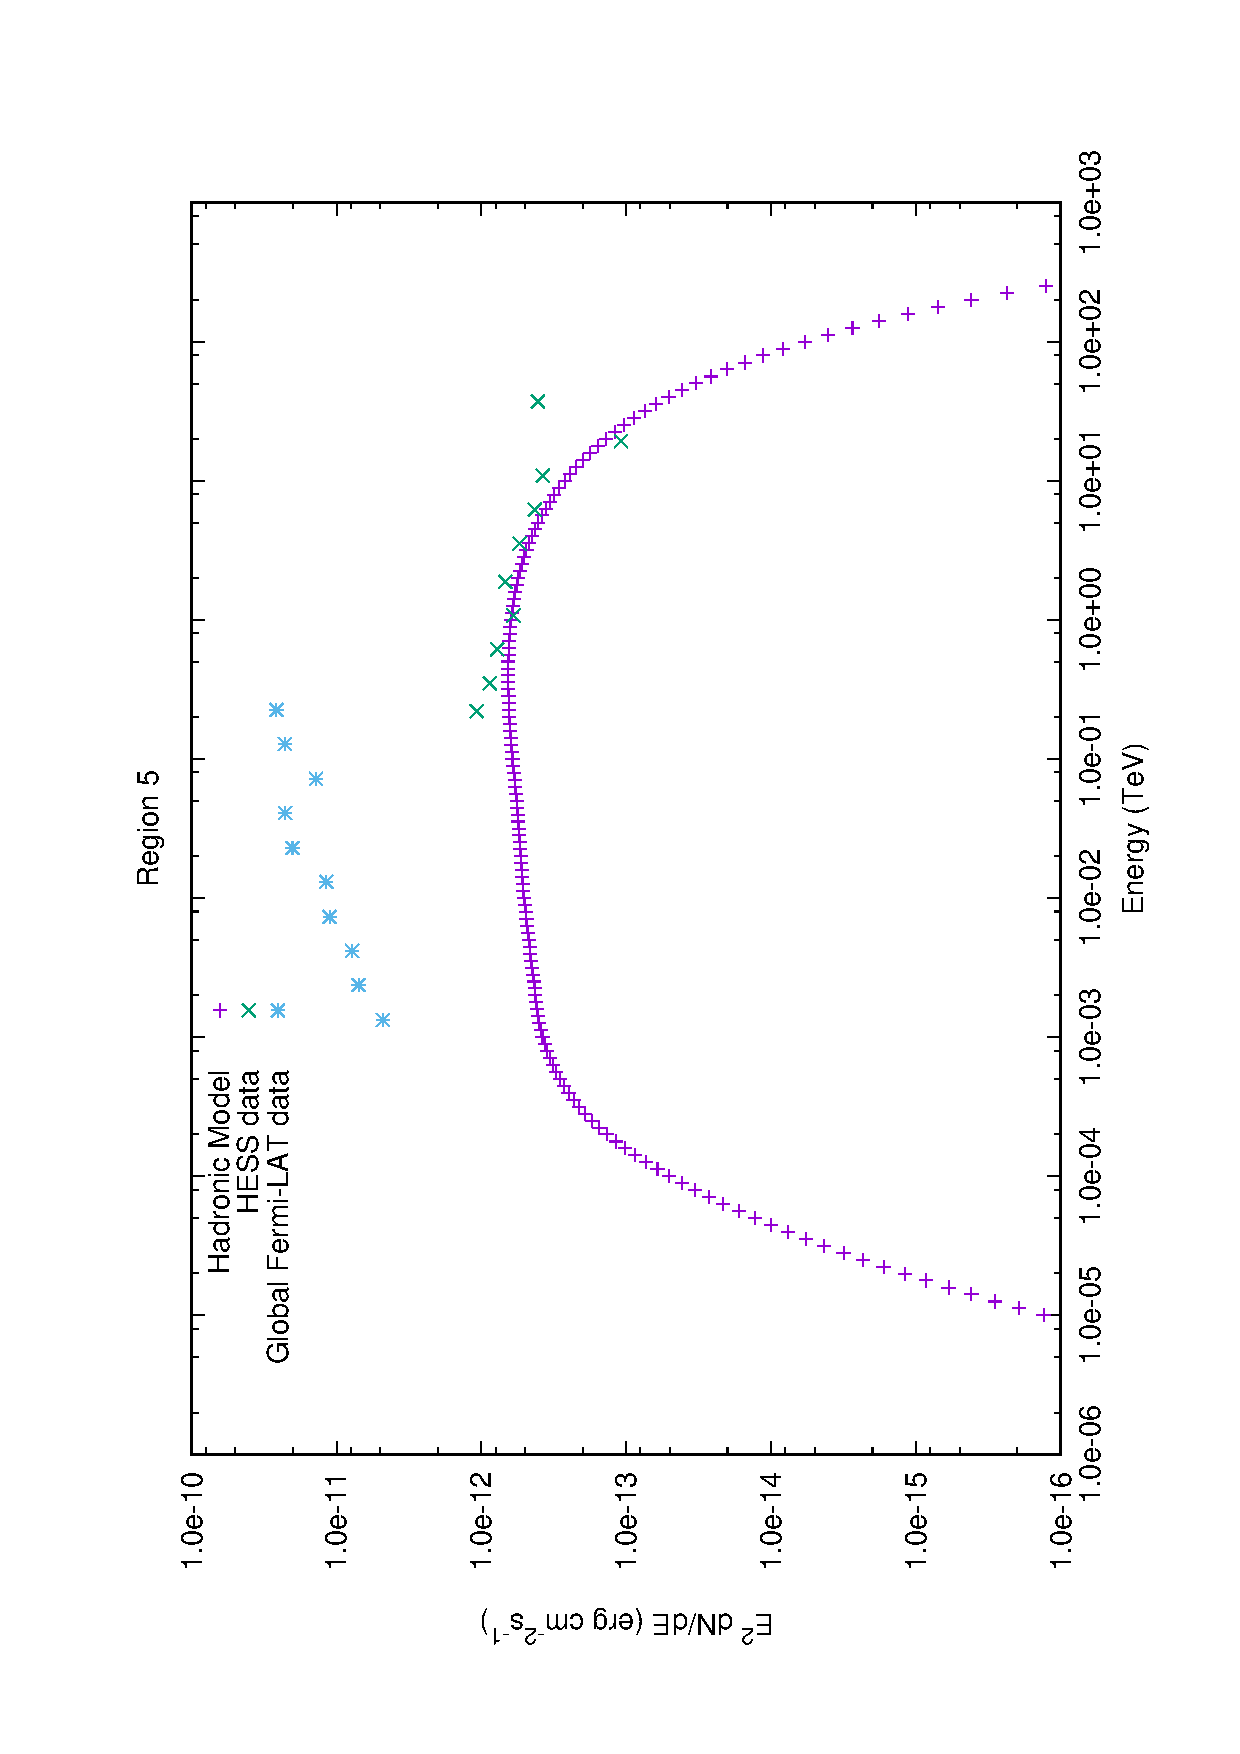
\includegraphics[width=0.7\linewidth, height=0.27\textheight, angle=-90]{rxj1713_had5}
		\label{fig:rxj1713lephad5}
	\end{subfigure}
	\begin{subfigure}{0.5\textwidth}
		\centering
		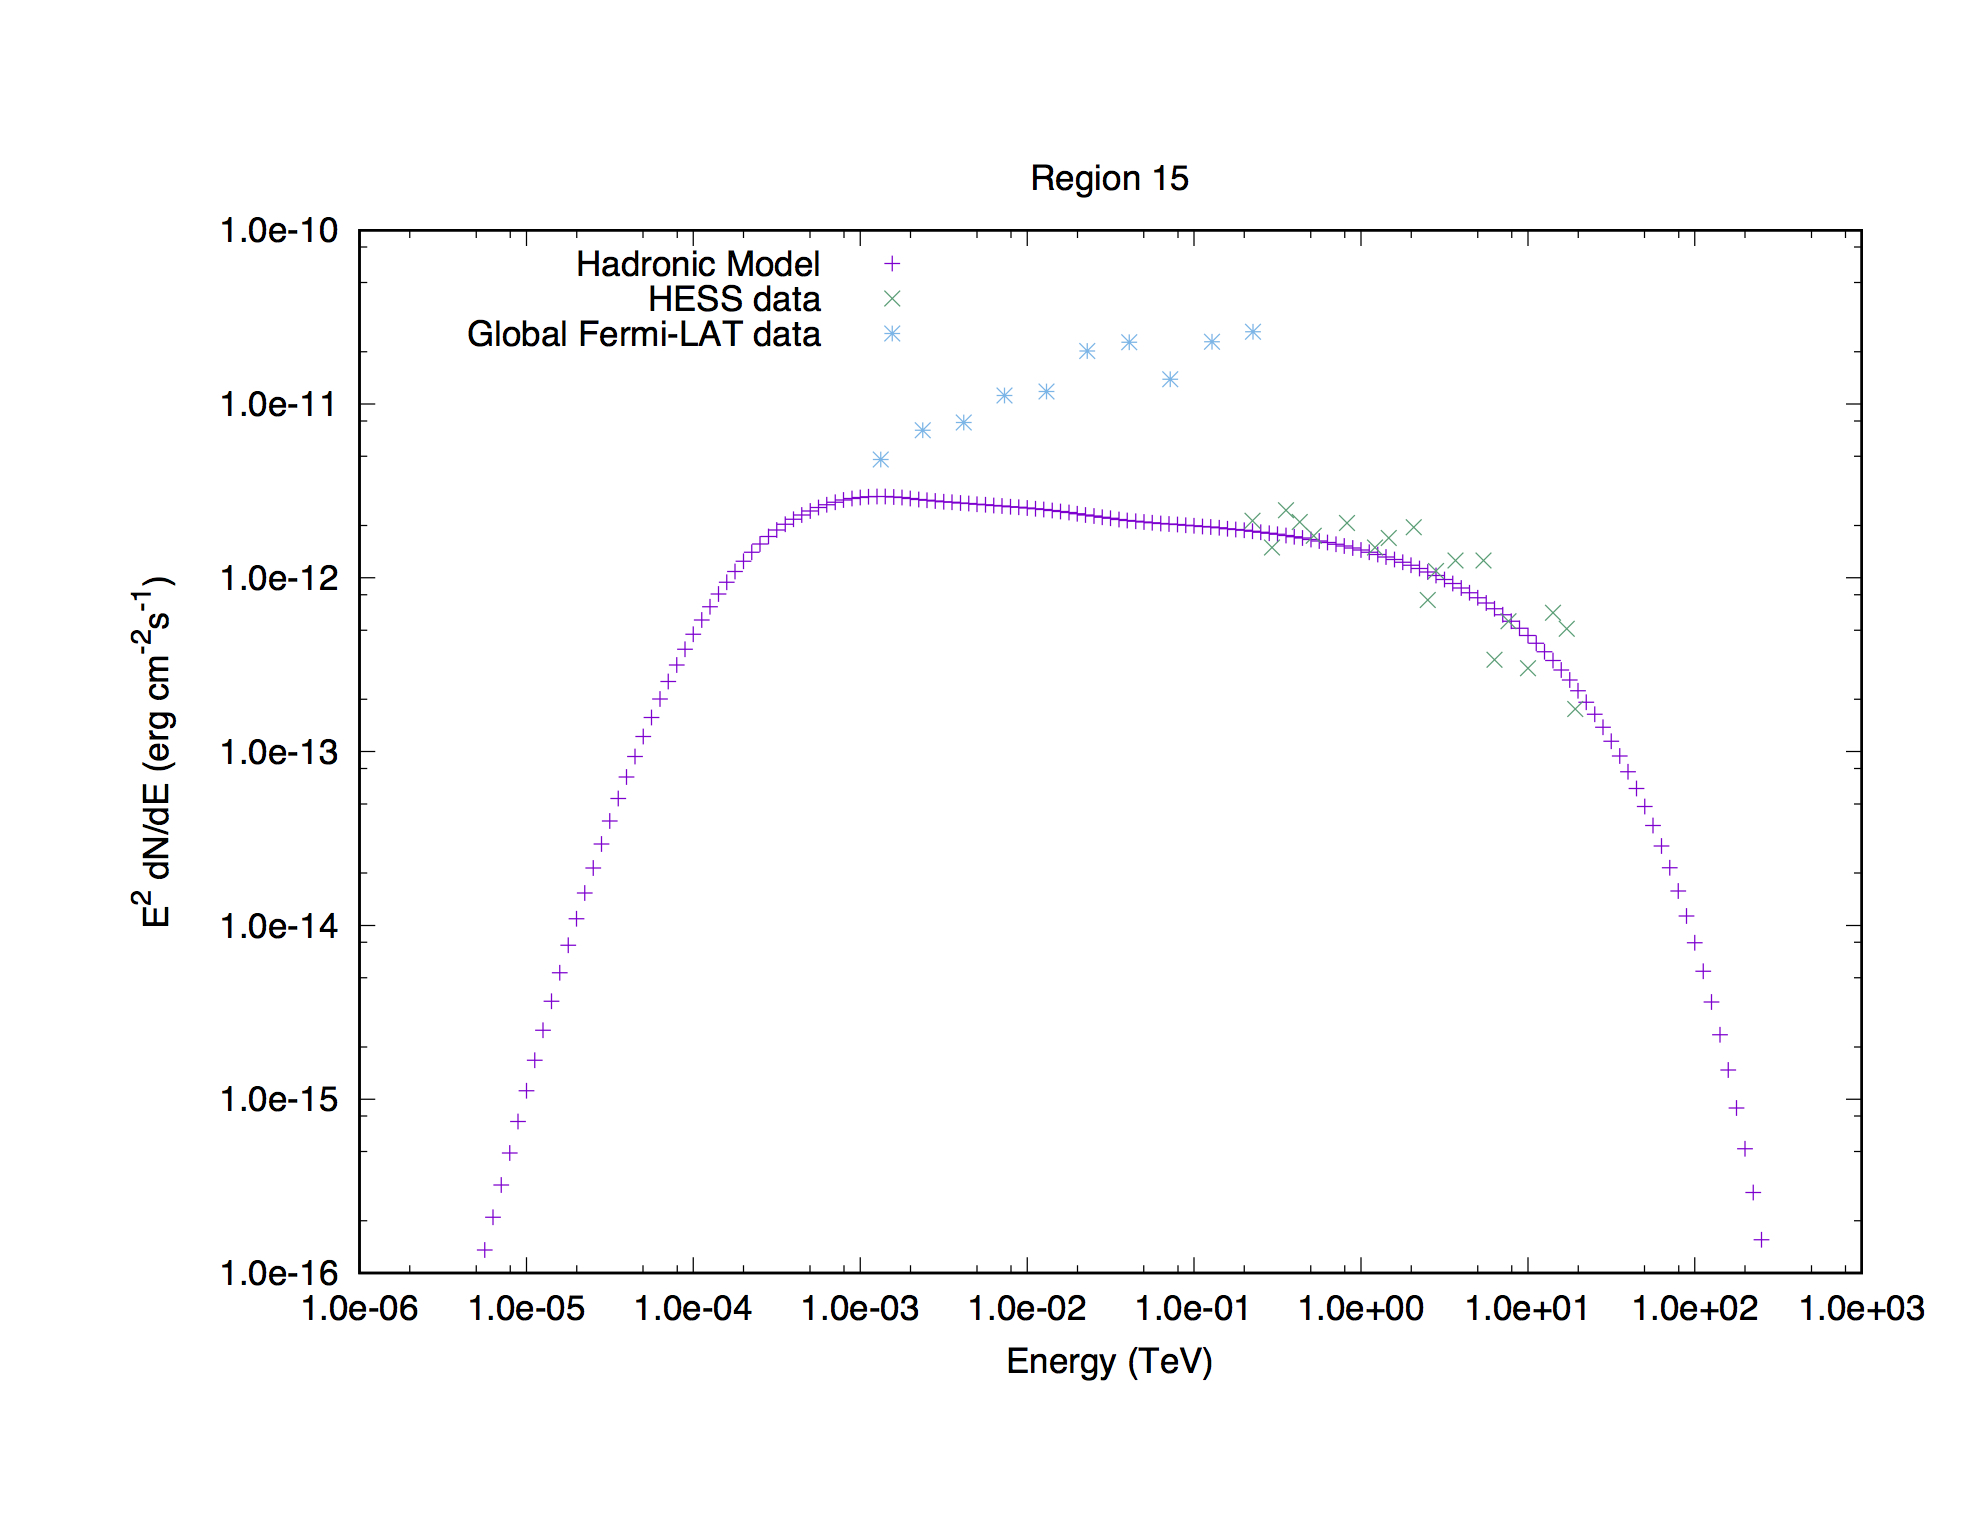
\includegraphics[width=0.7\linewidth, height=0.27\textheight, angle=-90]{rxj1713_had15}
		\label{fig:rxj1713lephad15}
	\end{subfigure}
	\begin{subfigure}{0.5\textwidth}
		\centering
		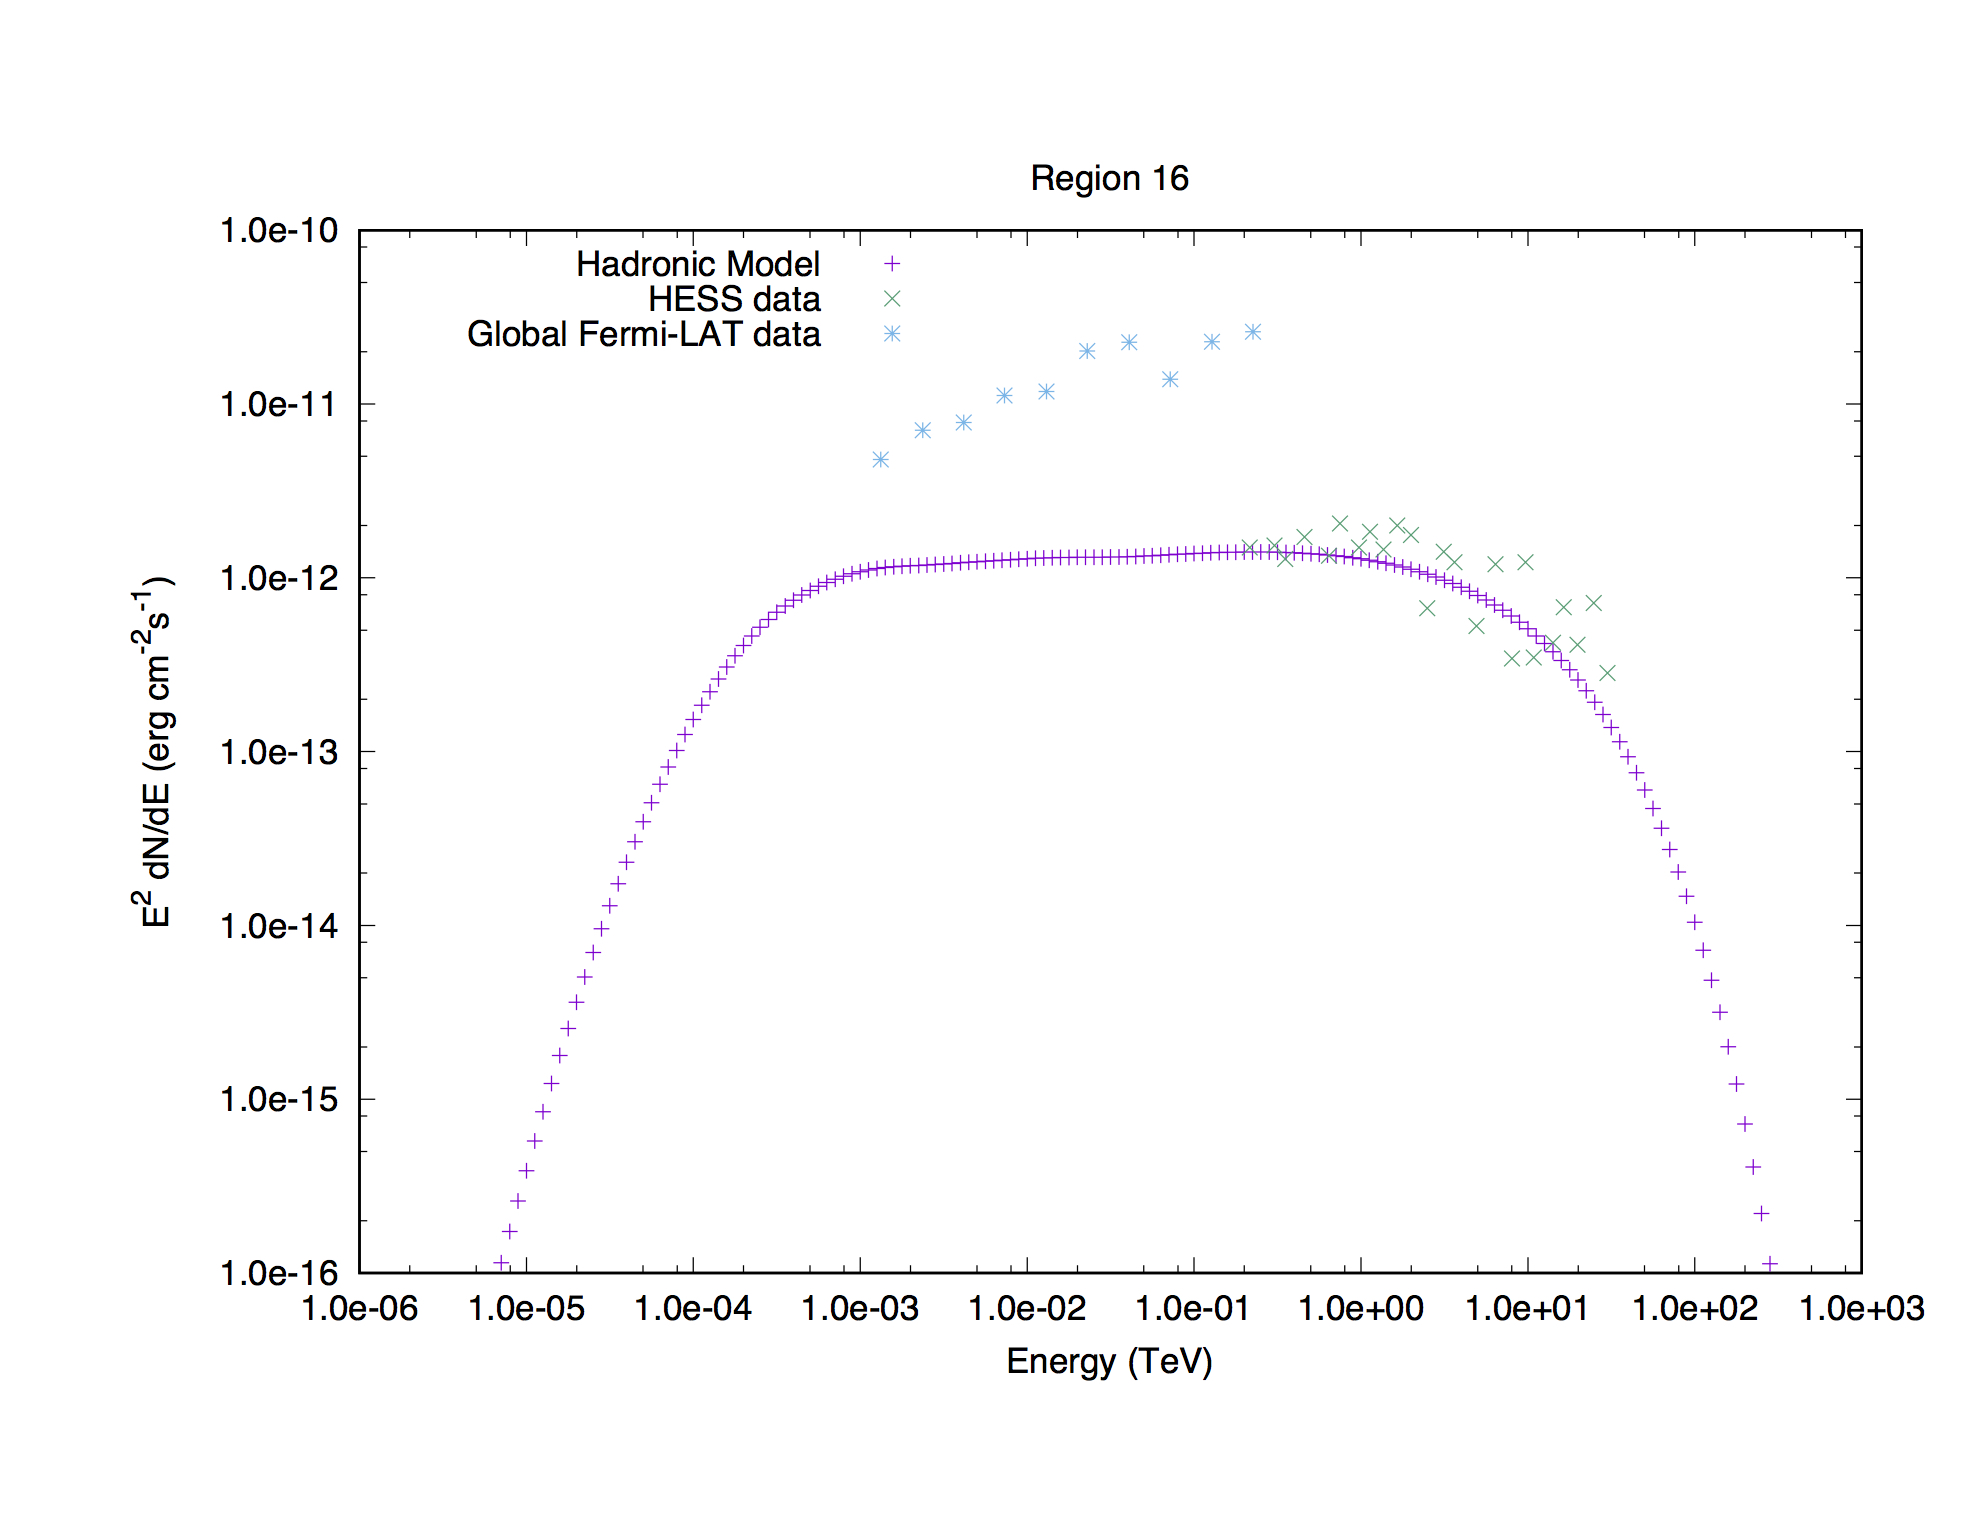
\includegraphics[width=0.7\linewidth, height=0.27\textheight, angle=-90]{rxj1713_had16}
		\label{fig:rxj1713lephad16}
	\end{subfigure}
	\begin{subfigure}{0.5\textwidth}
		\centering
		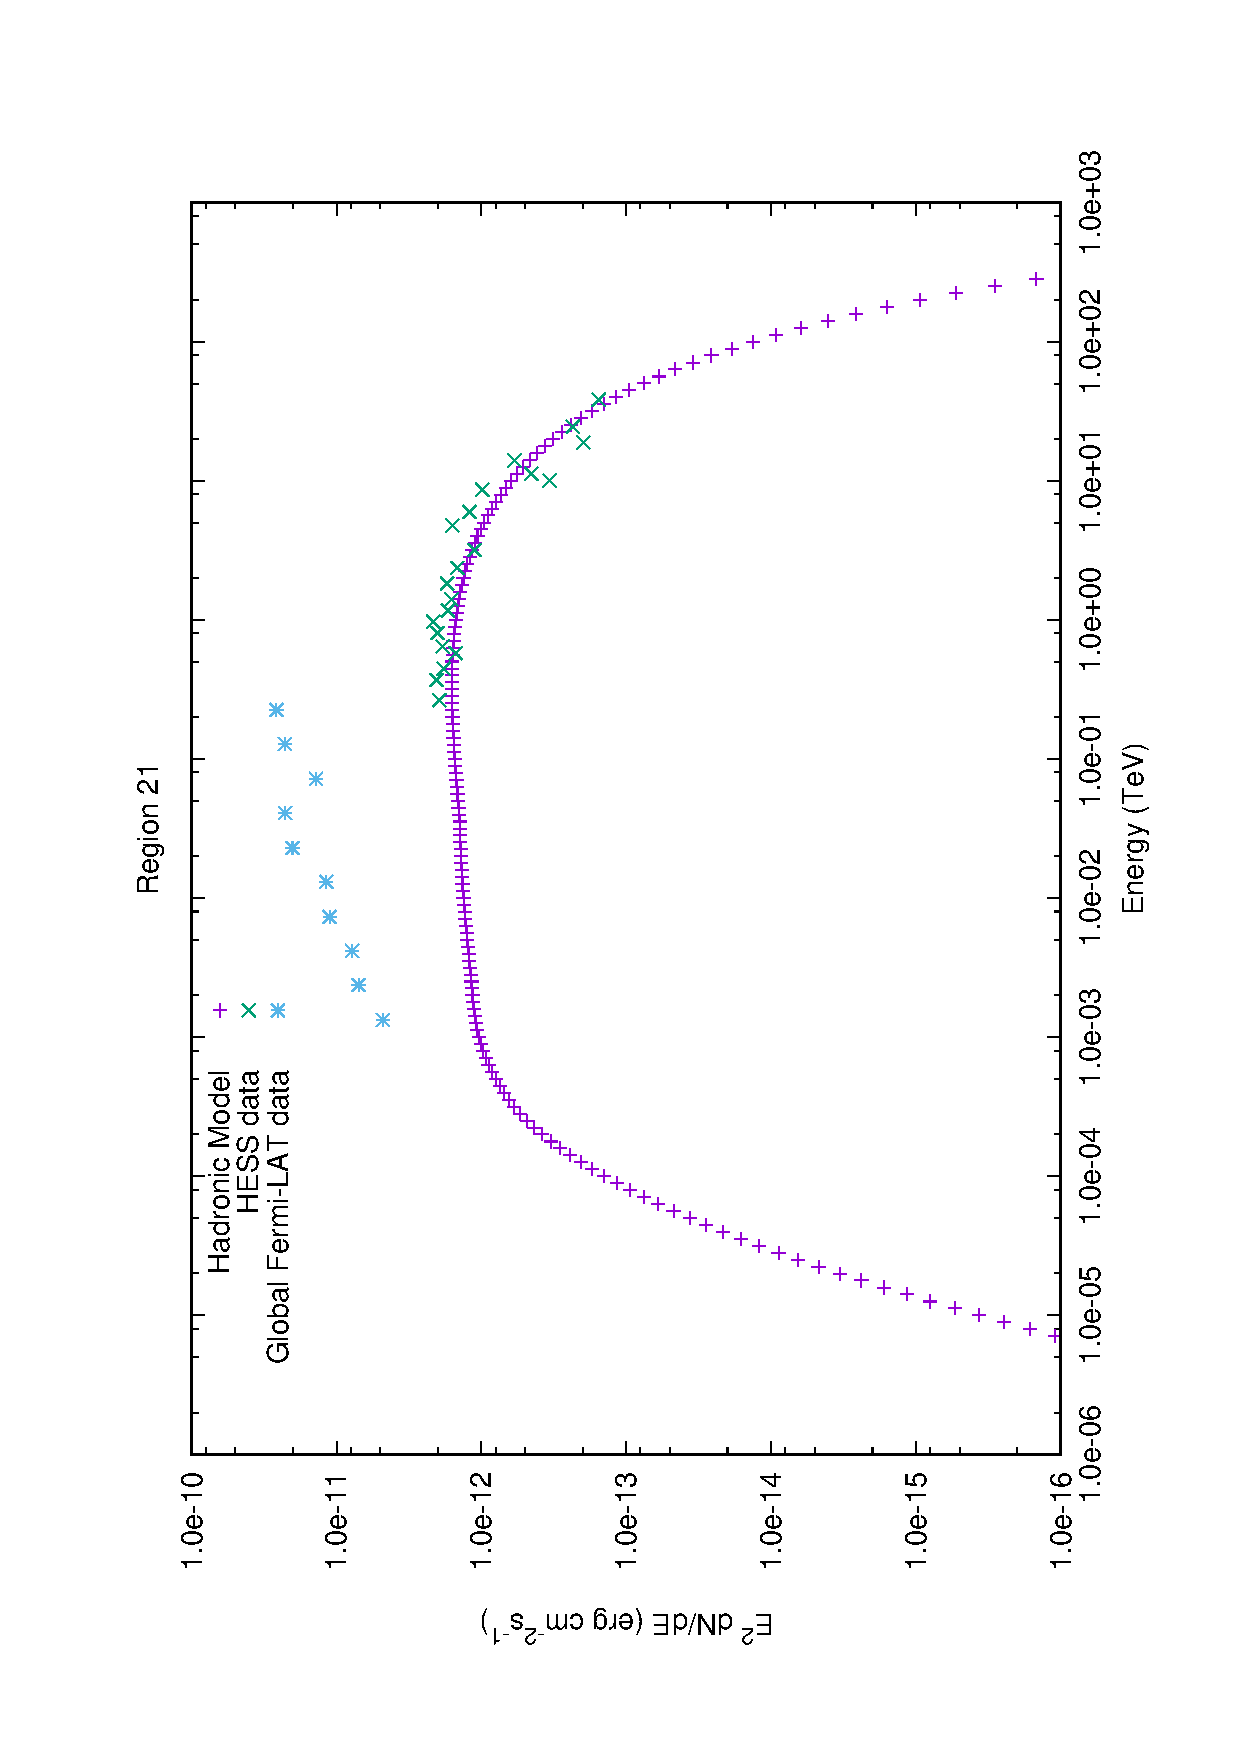
\includegraphics[width=0.7\linewidth, height=0.27\textheight, angle=-90]{rxj1713_had21}
		\label{fig:rxj1713lephad21}
	\end{subfigure}
	\begin{subfigure}{0.5\textwidth}
		\centering
		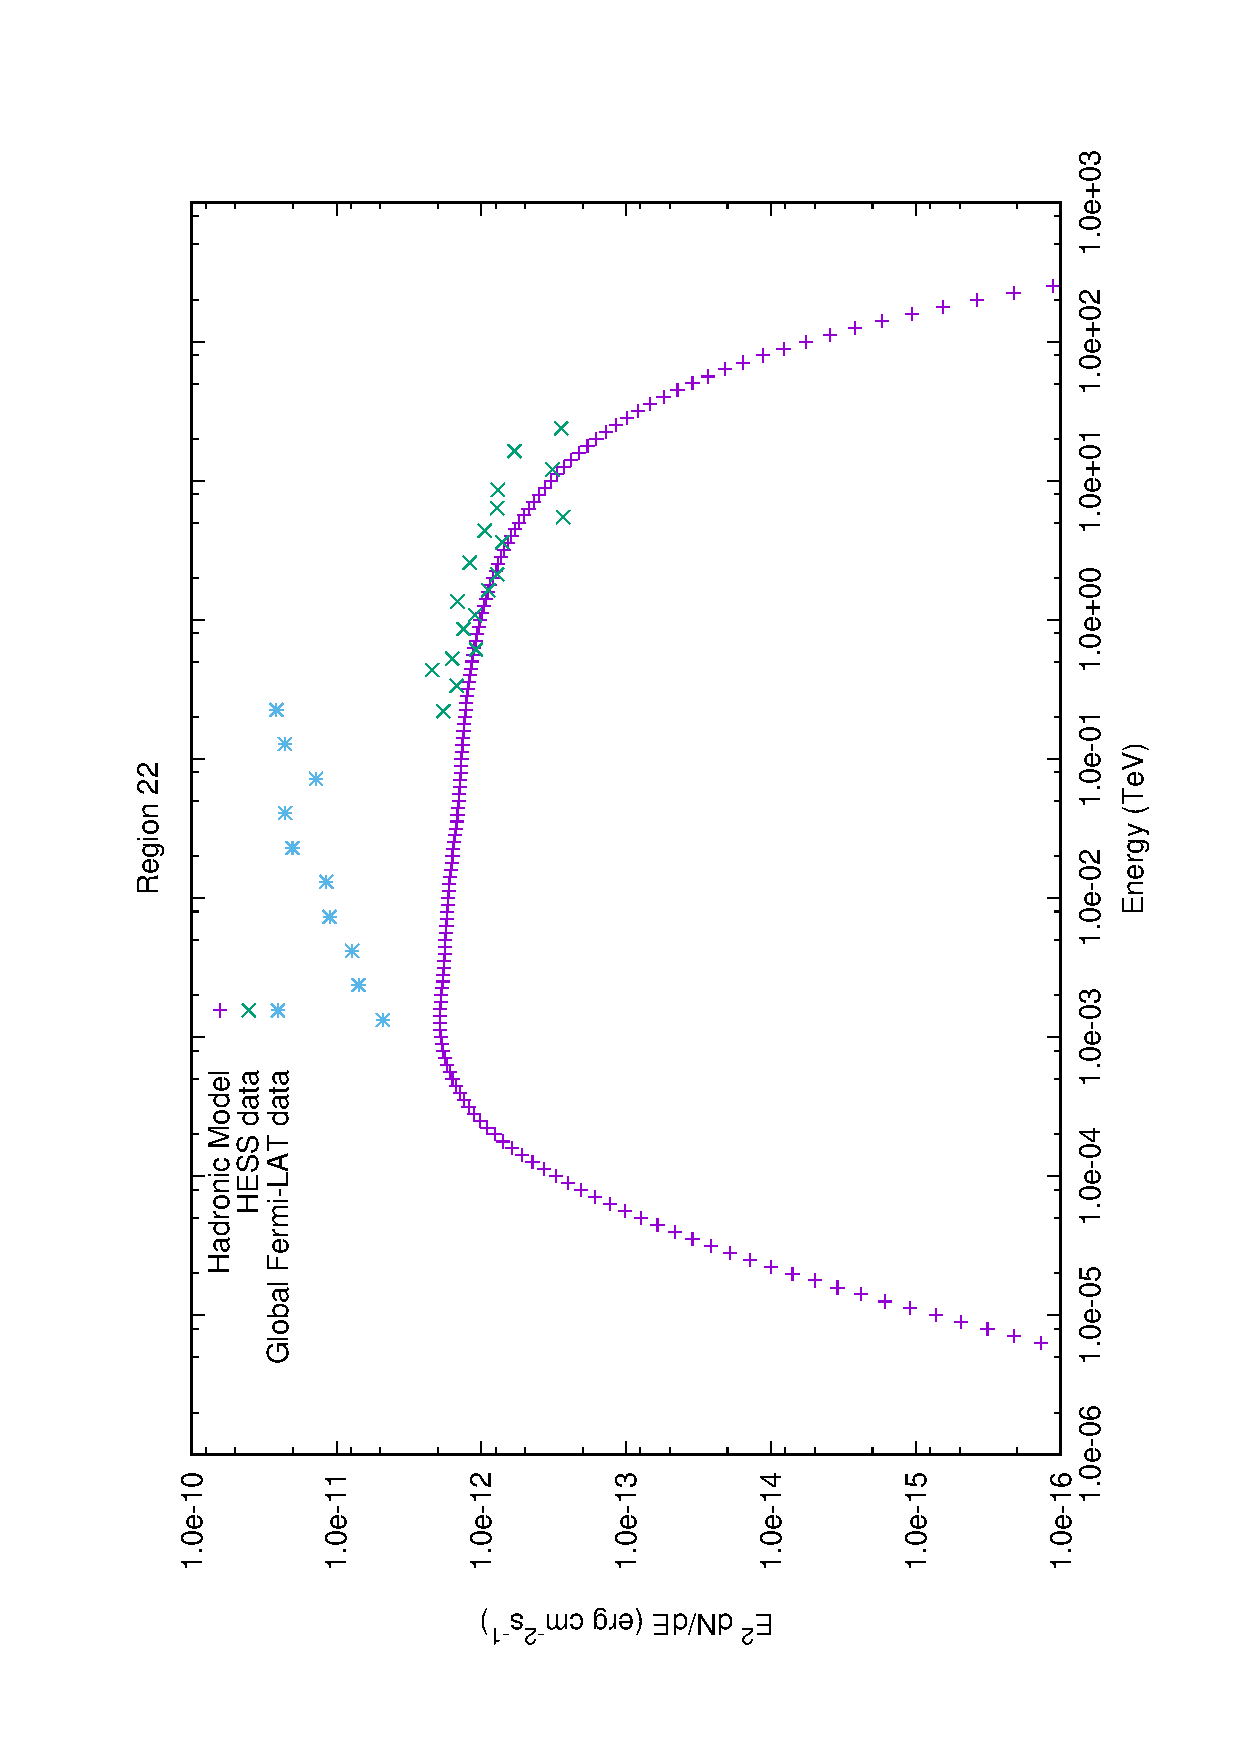
\includegraphics[width=0.7\linewidth, height=0.27\textheight, angle=-90]{rxj1713_had22}
		\label{fig:rxj1713lephad22}
	\end{subfigure}
	\begin{subfigure}{0.5\textwidth}
		\centering
		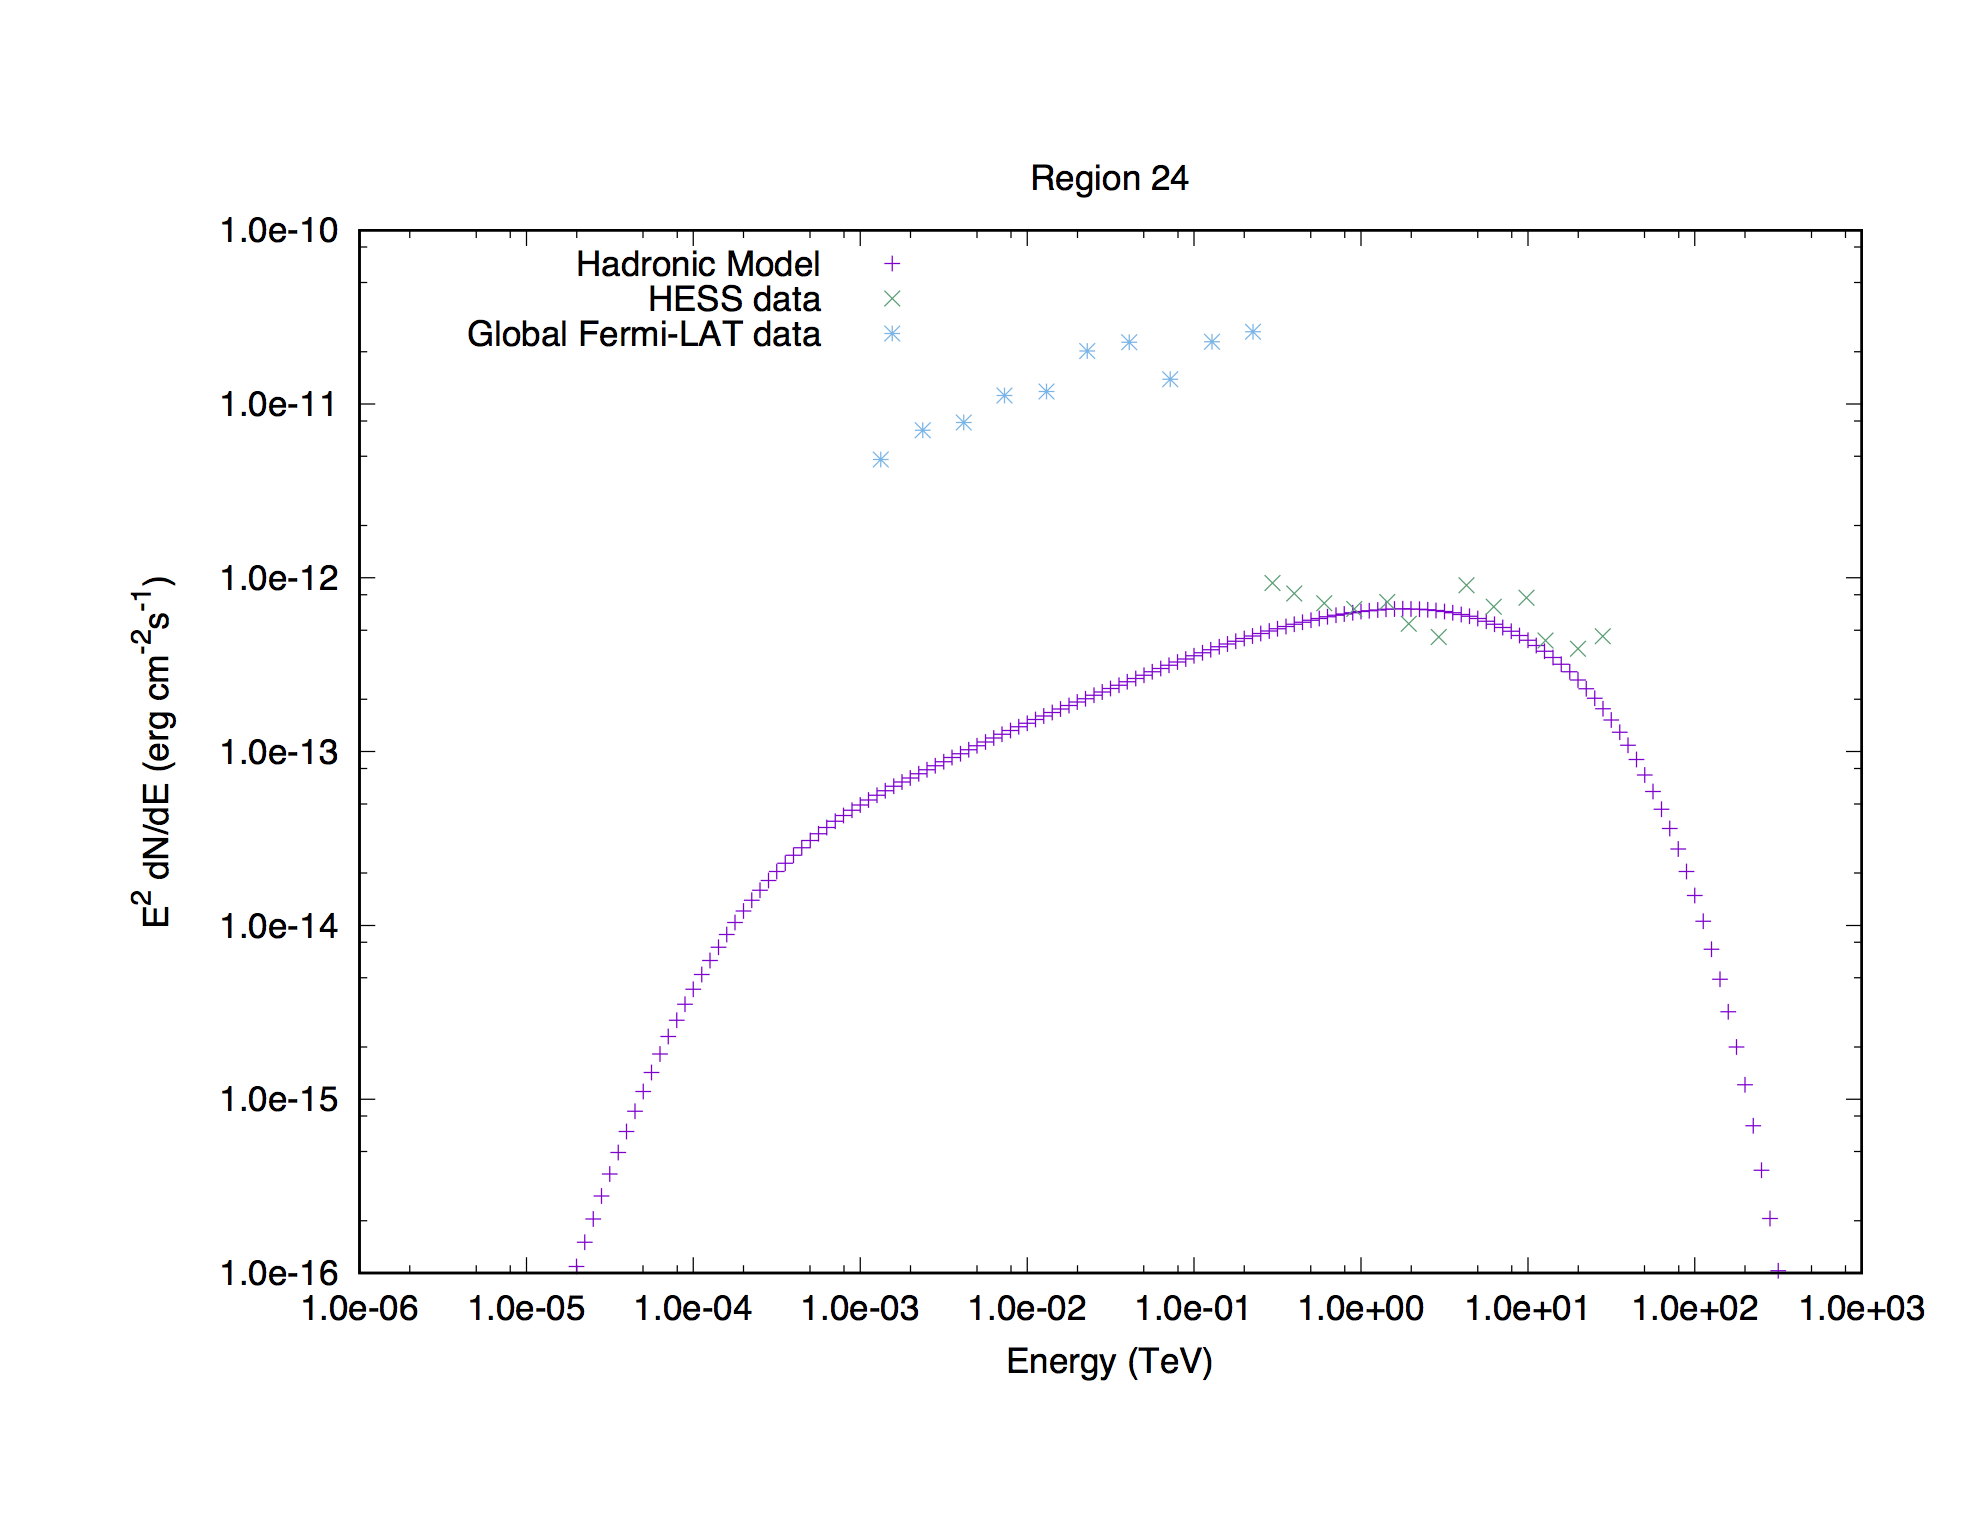
\includegraphics[width=0.7\linewidth, height=0.27\textheight, angle=-90]{rxj1713_had24}
		\label{fig:rxj1713lephad24}
	\end{subfigure}
	\caption{Hadronic SEDs for 6 regions within RX J1713.7-3946}
	\label{fig:regionalhadseds}
\end{figure}
The Fermi-LAT upper limit data (and the HESS global data) should agree with a cumulative sum of all the modeled spectra at any given energy. Figure \ref{fig:hadcumsum} illustrates the cumulative sum of the spectra from each region compared to the global data. Firstly, we note that this cumulative sum model fits the HESS data well. However, it can clearly be seen that in the GeV energy range (up to about 200 GeV) this cumulative sum overpredicts the Fermi-LAT observations. This could be a result of the data fitting. Due to the lack of observations to fit to in the GeV energy range, there is nothing to restrict the spectra on a regional level. An energy break could be applied to the models for each region to decrease the amount of low energy protons interacting with the ISM gas. This would ultimately only affect the low energy tail of the spectra, whilst maintaining the spectral fits to the HESS data, providing us with a better cumulative fit. However, assigning a low energy spectral index would be ambiguous and have no physical meaning with no data to fit to in the GeV range to begin with. Alternatively, the hadronic SED model may not be complete. \cite{2014MNRAS.445L..70G} explain how lower energy CRs would have limited interactions if a clumpy medium were present in the shock environment. These small, dense, clumpy regions stay intact after experiencing the SNR wind and remain as target gas for the CR protons, while the remainder (and majority) of the medium gets blown away leaving a low density gas surrounding the clumps. Higher energy CRs will be more likley to penetrate these dense clumps, while lower energy CRs will be bounced away by the intense magnetic fields present in the clumps. What we model in this work is a much larger region, which takes the average density of the clumps and low density surrounding gas. This assumes that our entire population of CRs are interacting with most of the gas and hence may overpredict the $\gamma$-ray emission from the low energy protons. What we may need is some sort of supression factor that handles this problem but for now it is beyond the scope of the work. Finally, it could be that these regions that appear to be violating the upper limit are simply not described well by a hadronic model and will need further investigation with either a leptonic model or combined model. The hadronic nature of these regions is investigated further in a gas-$\gamma$-ray flux correlation study below. 

\begin{figure}[H]
	\centering
	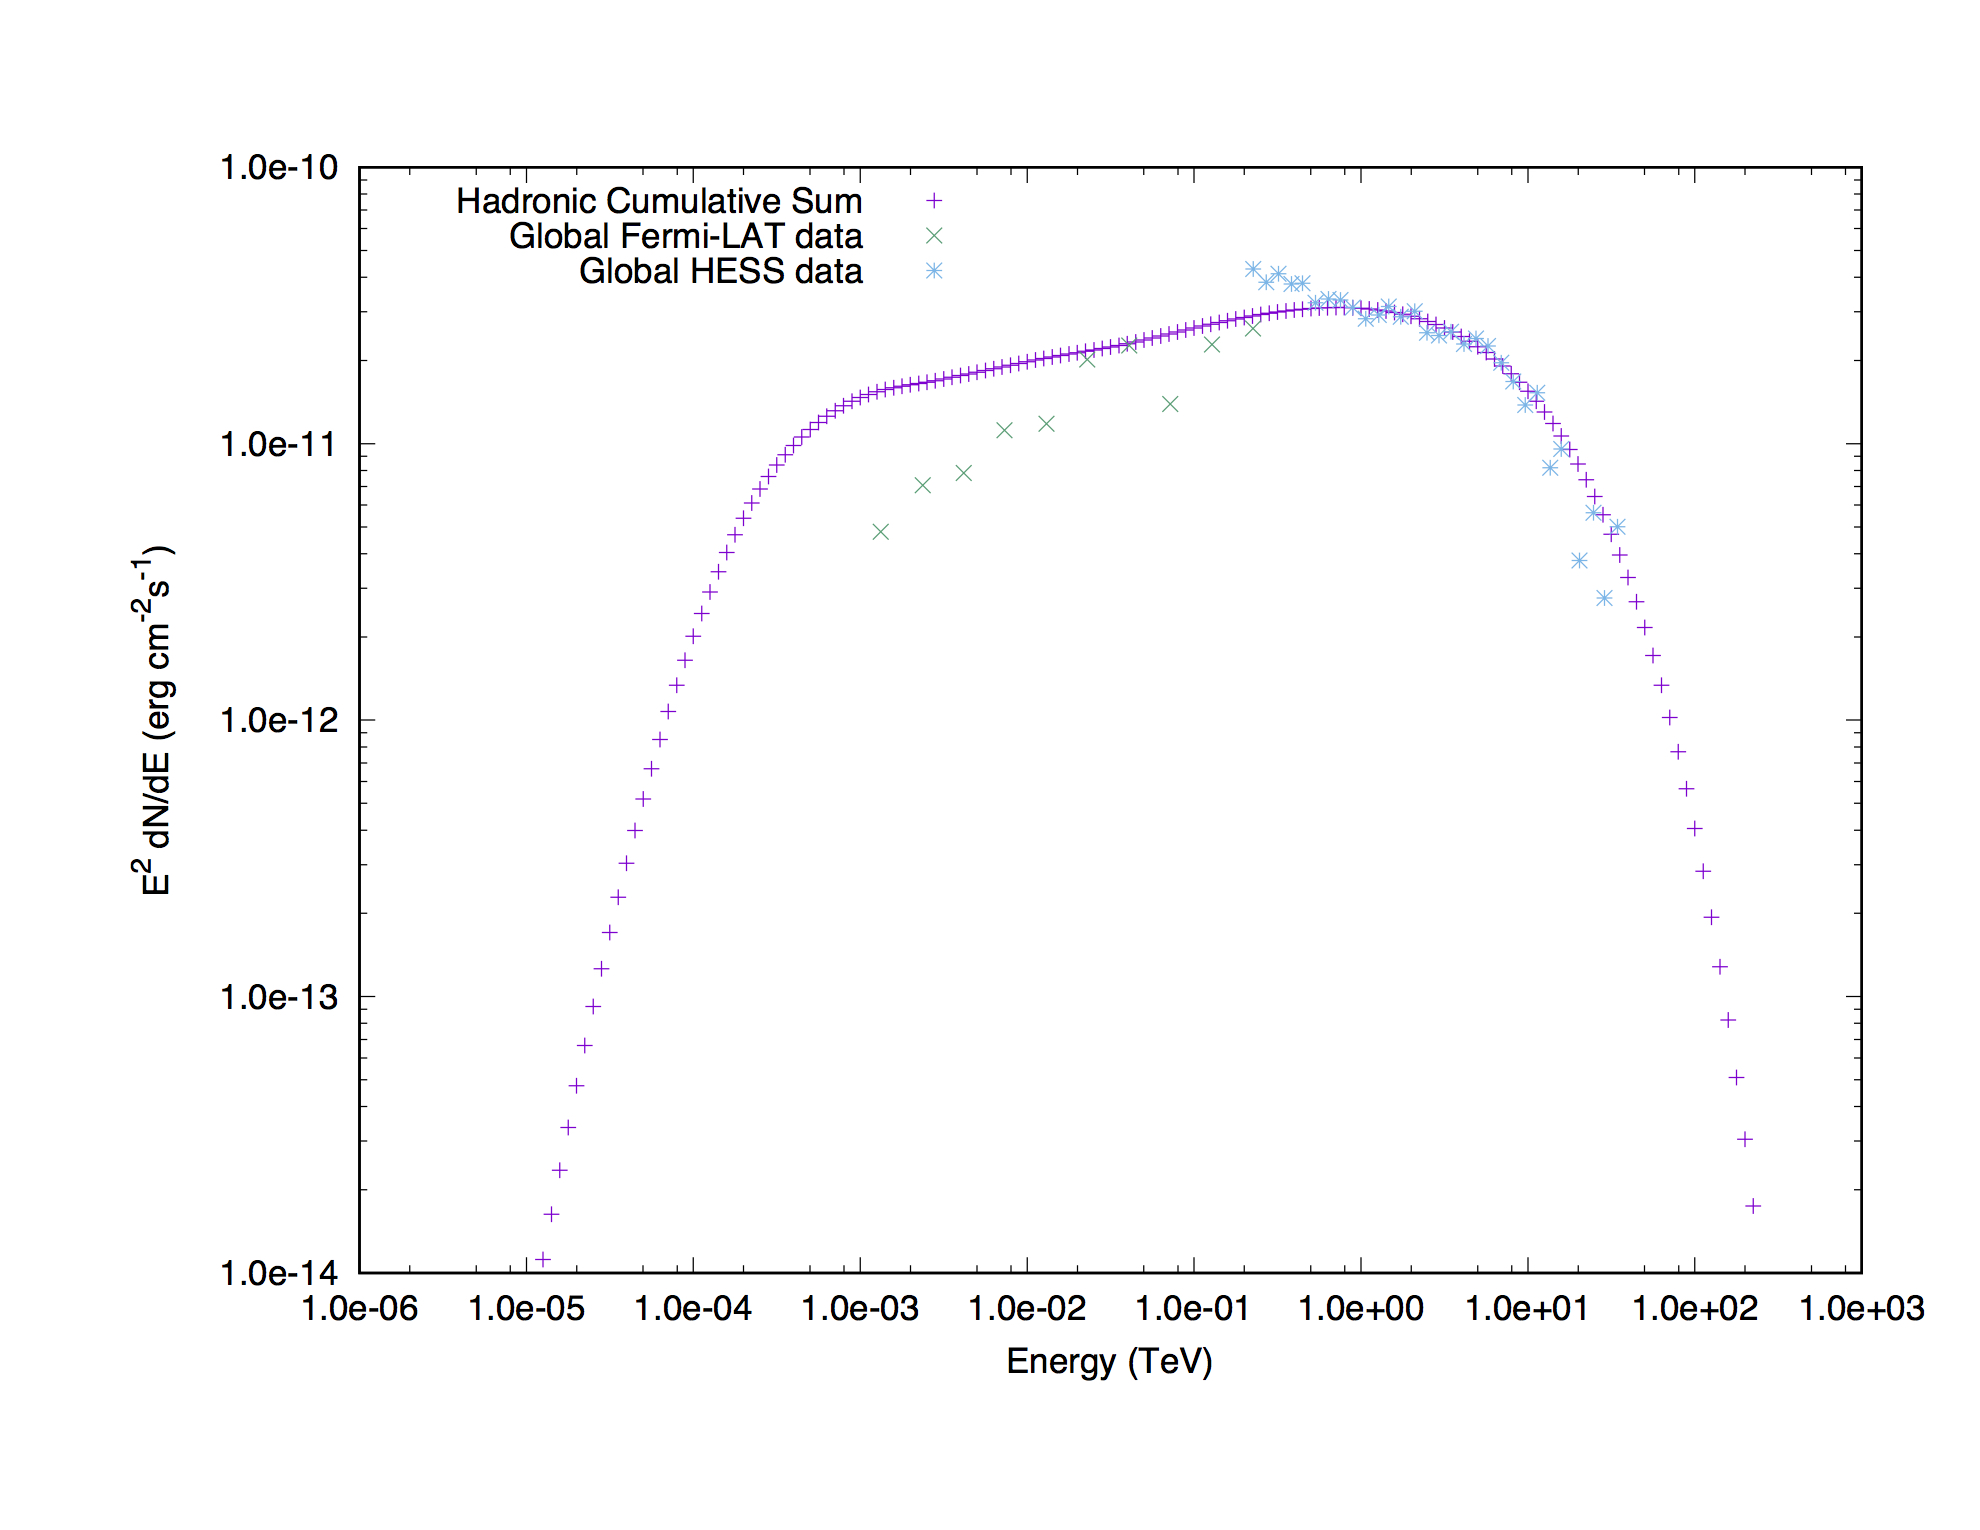
\includegraphics[width=0.4\linewidth, height=0.3\textheight, angle=-90]{rxj1713_had_cumsum}
	\caption{Cumulative sum of the hadronic spectra from each region with the Fermi-LAT and HESS data points for the entire SNR region.}
	\label{fig:hadcumsum}
\end{figure}

The modeled SED injection energy's, $W_{p,\mathrm{SED}}$, ranged from $1.06 \times 10^{46} - 15.22 \times 10^{46}$ erg across the regions. To investigate the accuracy of these injection energies we compared against two different theoretical calculations. 

\subsubsection{$\mathbf{10^{50}}$ erg Energy Budget Model}
Firstly, we exploited the theoretically expected $10^{50}$ erg energy budget for CRs in SNRs \ref{} and divided this between the regions. Assuming these CRs are isotropically distributed within a spherical shaped bubble the size of our entire SNR region, each region receives a slightly different fraction of this energy. The amount of energy injected into each region scales according to its volume filling factor ($V_{ff}$) within the bubble. The $V_{ff}$ depends on the regions position on the surface of the sphere and followed a similar analysis to that of section \ref{sec:regdenscalc}. Table \ref{tab:regionalvolumes} shows the depth and $V_{ff}$ of each region, which were used to calculate the total fractional injection energy, $W_{p,50,\mathrm{T}}$, for each region. 
\begin{table}[H] 
	\begin{center}
		\begin{tabular}{cccc}
			\toprule
			Depth (pc) & $V_{ff}$ &  $W_{p,50,\mathrm{T}}$ ($10^{48}$erg) & Regions \\
			\hline
			12.8 & 0.026 & 2.61 & 1, 4, 5, 10, 22, 23, 28, 29 \\
			16.0 & 0.033 & 3.27 & 2, 3, 6, 11, 16, 17, 24 \\
			19.2 & 0.039 & 3.92 & 7, 8, 9, 12, 15, 18, 19, 20, 21, 25 26, 27 \\
			22.4 & 0.046 & 4.58 & 13, 14 \\
			\bottomrule
		\end{tabular} 
	\end{center}
	\caption{Column depth into the SNR, volume filling factor and fractional injection energy, based on the $10^{50}$ erg budget, for each region.}
	\label{tab:regionalvolumes}
\end{table}
Additionally, we ignored the energy accounted for from CR protons that have escaped the SNR. We normalised the fractional injection energy assuming protons of energy 150 TeV and above had already escaped (equation \ref{eq:normescape}) to find the theoretical proton injection energy $W_{p,50}$. 
\begin{equation}\label{eq:normescape}
W_{p,50} = W_{p,50,\mathrm{T}}\mathrm{(<150TeV)} = \dfrac{W_{p,50,\mathrm{T}}}{\int_{\mathrm{E_0}}^{\infty}  E^{-\alpha + 1} dE}\int_{E_0}^{150 \ \mathrm{TeV}}  E^{-\alpha + 1} dE\\
\end{equation}
A comparison of $W_{p,50}$ (table \ref{tab:hadronicparams}) with the modeled energy's, $W_{p,\mathrm{SED}}$, showed that the SED models are up to 2 magnitudes of order less than $W_{p,50}$. A drastic implication of the low SED injection energies could be that the hadronic models were not sufficient to explain the $\gamma$-ray flux in each region. Alternatively, the assumption that the CRs have an energy budget of $10^{50}$ erg could be incorrect. It wouldn't be unphysical for RX J1713.7-3946 to have a smaller than expected amount of energy injected into CRs. \cite{2017ApJ...837...36L} showed that Supernovas in the Large Magellanic Cloud could expel as little as $0.04 \times 10^{51}$erg into their explosions. Subsequently the CRs would only receive 10\% of this energy, e.g. as little as $4 \times 10^{48}$ erg. This is about 2 orders of magnitude less than what we assumed when calculating $W_{p,50}$. 

The cumulative sum of $W_{p,\mathrm{SED}}$ across all regions was calculated to be $1.25 \times 10^{48}$ erg, this is comparable to the result from \cite{2017ApJ...837...36L} ($4 \times 10^{48}$ erg). Suggesting that the hadronic SED models are acceptable. Additionally, the assumption that 10\% of the explosion energy is imparted to CRs may not be accurate. If the SNR source at RX J1713.7-3946 did have a small explosion energy and less than 10\% of this energy was received by the CRs then our SED models would be comparable to $W_{p,50}$. Furthermore, compared to the H16 model of the entire SNR ($W_p = 6.55 \times 10^{47}$ erg), we found that our cumulative sum over-predicts this value only by a factor of 2. This leads us to believe that our SED models were physically sound within the literature just mentioned if we assume a smaller explosion energy is allowed. However, our theoretical $W_{p,50}$ values may not be valid. We could conclude that our SNR source has the aforementioned characteristics or we can attempt to predict the proton injection energy using a different method.

\subsubsection{HESS Flux Data and Cooling Time Model}
An alternative technique for predicting the injection energy for each region utilises the HESS $\gamma$-ray spectral data. These energy flux points were integrated (equation \ref{eq:fluxsum}) to obtain the total $\gamma$-ray flux, $F_{\gamma}$, within the energy range imposed by the data ($E_{max}$ and $E_{min}$). 
\begin{equation}\label{eq:fluxsum}
F_\gamma = \int_{E_{min}}^{E_{max}} F_{\gamma, i} \dfrac{1}{E_i} dE \ \mathrm{erg\ cm}^{-2} \ \mathrm{s}^{-1}
\end{equation}
where $F_{\gamma, i}$ and $E_i$ are the $\gamma$-ray flux and energy, respectively, corresponding to the ith data point. The total $\gamma$-ray flux was then converted into a luminosity, $L_\gamma$, by multiplying by $4 \pi d^2$, where $d$ is the distance to our source (1 kpc). The density dependent cooling time, $t_{pp}$, for p-p interactions (equation \ref{eq:cooltimeshad}) was then multiplied by the luminosity to obtain a predicted injection energy, $W_{p,\mathrm{cool}}$. These last 2 steps are summarised in equation \ref{eq:fluxtoinject}.
\begin{equation}\label{eq:fluxtoinject}
W_{p,\mathrm{cool}} = t_{pp} \times L_\gamma = t_{pp} \times 4 \pi d^2 \times F_\gamma 
\end{equation}
The region-dependent calculations of $t_{pp}$ can be found in table \ref{tab:ppcooltimes}.
\begin{table}[H] 
	\begin{center}
		\begin{tabular}{cccccccc}
			\toprule
			Reg. & $t_{pp}$ ($\times 10^5$ years) && Reg. & $t_{pp}$ ($\times 10^5$ years) && Reg. & $t_{pp}$ ($\times 10^5$ years)\\ 
			\hline 
			1& 5.06 && 11 & 5.21  && 21 & 3.33 \\ 
			2& 4.97 && 12 & 6.16  && 22 & 2.93 \\ 
			3& 3.72 && 13 & 7.41  && 23 & 6.74 \\ 
			4& 4.72 && 14 & 5.99  && 24 & 7.41 \\ 
			5& 7.56 && 15 & 4.84 && 25 & 6.77  \\ 
			6& 5.47 && 16 & 3.50  && 26 & 6.14 \\ 
			7& 7.47 && 17 & 6.73  && 27 & 3.27 \\ 
			8& 5.20 && 18 & 7.76  && 28 & 5.40 \\ 
			9& 3.48 && 19 & 8.11  && 29 & 4.00 \\ 
			10& 3.39 && 20 & 7.19  && & \\ 
			\bottomrule
		\end{tabular} 
	\end{center}
	\caption{The calculated proton density for each region towards RX J1713.7-3946.}
	\label{tab:ppcooltimes}
\end{table}

The predictions, $W_{p,\mathrm{cool}}$, can be found in table \ref{tab:hadronicparams}. The HESS data only covered a limited energy range ($\approx$ 0.1 TeV to 30 TeV), so $W_{p,\mathrm{cool}}$ also only applies to that energy range. For comparison, the SED modeled injection energy for each region were normalised to match this energy range ($W_{p, \mathrm{SED}, \mathrm{TeV}}$) and are shown in table \ref{tab:hadronicparams}. Table \ref{tab:hadronicparams} also shows the ratio, $R_{\mathrm{cool/SED}}$, of the predicted injection energy, $W_{p, \mathrm{cool}}$, to the SED modeled $W_{p,\mathrm{SED}, \mathrm{TeV}}$.

It is important to note that all regions were over-predicted by $W_{p, \mathrm{cool}}$ compared to $W_{p, \mathrm{SED}, \mathrm{TeV}}$. This could be explained by the Riemann sum method of integration. The HESS $\gamma$-ray flux generally decrease in intensity as energy increases and because the integration begins at the lowest energy bin, each infinitesimal rectangle will be overestimating the likely flux (see appendix). Additionally, the $\gamma$-ray flux that HESS observed is a snapshot of the whole lifetime of the SNR. When we apply the cooling time to our calculation we assume that all of the CR protons have radiated their energy away in PP interactions. Since we are observing the SNR before this cooling time has been reached, our predications are overestimating what we see. Another assumption we make when using the cooling time to calculate $W_{p,\mathrm{cool}}$, is that all the CR protons collide with and interact with all the gas. It is more likely that a fraction of these protons actually interact with the gas. This could help explain why we over-predicted $W_{p,\mathrm{cool}}$, compared to $W_{p,\mathrm{SED}, \mathrm{TeV}}$. 

Furthermore, the discrepancies between $W_{p,\mathrm{cool}}$ and $W_{p,50}$ are not easy to decipher, unless our assumptions we used to calculate $W_{p,50}$ are incorrect, as discussed earlier. The fact that $W_{p,\mathrm{cool}}$ agrees well with $W_{p,\mathrm{SED}, \mathrm{TeV}}$ leads us to believe that $W_{p,50}$ was indeed incorrectly calculated. This also gives us reason to believe that the hadronic SED model is partly successful in predicting the $\gamma$-ray flux from our 29 regions. We say partly successful because numerous regions have a ratio $>$ 10, which flags our attention that maybe the hadronic model is not solely sufficient to explain the $\gamma$-ray flux in these regions. Further investigation is required for the regions with large ratios. Otherwise, $W_p$ was predicted well using this 2nd technique, most regions had a value within a factor of 10 compared to the SED models. Regions 15, 16, 21 and 22, which we showed to be potentially violating the Fermi-LAT upper limit earlier in our SED modeling, all seem to have a low $R_{\mathrm{cool/SED}}$ value ($< 10$). We can begin to conclude for these regions that a hadronic component is important in explaining the $\gamma$-ray flux, however we may need corrections to our SED model, especially at low energies. Overall we can conclude that some of our hadronic SED models require injection energies that are valid within the scope of the theory and observations but still require further clarification. We can also begin to conclude that those regions with large $R_{\mathrm{cool/SED}}$ values may not have a significant hadronic component at all.

\begin{table}[H] 
	\begin{center}
		\begin{tabular}{cccccccc}
			\toprule
			&
			\multicolumn{4}{c}{($\times 10^{46}$ erg)} 
			&&&
			\\ \cline{2-5}
			Reg. & $W_{p,\mathrm{SED}}$ & $W_{p,50}$ & $W_{p,\mathrm{SED}, \mathrm{TeV}}$ & $W_{p,\mathrm{cool}}$ & $R_{\mathrm{cool/SED}}$ & $\alpha$ & $n_H$(cm$^{-3}$)  \\
			\hline
			1 & 1.06 & 247 & 0.537 & 0.659 & 1.23 & 1.60 & 105 \\ 
			2 & 2.36 & 320 & 0.369 & 0.437 & 1.18 & 1.82 & 107 \\ 
			3 & 2.51 & 324 & 0.325 & 0.454 & 1.40 & 1.95 & 143 \\ 
			4 & 1.64 & 253 & 0.158 & 0.558 & 3.53 & 1.76 & 112 \\ 
			5 & 4.41 & 258 & 0.306 & 0.643 & 2.10 & 1.96 & 70 \\ 
			6 & 3.32 & 315 & 0.258 & 0.923 & 3.58 & 1.70 & 97 \\ 
			7 & 5.04 & 379 & 0.404 & 1.45 & 3.60 & 1.74 & 70 \\ 
			8 & 4.93 & 383 & 0.212 & 1.04 & 4.92 & 1.81 & 102 \\ 
			9 & 5.85 & 388 & 0.185 & 0.818 & 4.43 & 1.94 & 152 \\ 
			10 & 2.26 & 254 & 0.085 & 0.490 & 5.76 & 1.78 & 156 \\ 
			11 & 3.35 & 321 & 0.098 & 0.765 & 7.78 & 1.85 & 102 \\ 
			12 & 3.11 & 378 & 0.098 & 0.832 & 8.48 & 1.72 & 86 \\ 
			13 & 4.17 & 443 & 0.142 & 1.22 & 8.60 & 1.74 & 72 \\ 
			14 & 4.64 & 450 & 0.133 & 1.37 & 10.3 & 1.87 & 88 \\ 
			15 & 15.22 & 391 & 0.270 & 0.972 & 3.61 & 2.14 & 110 \\ 
			16 & 5.19 & 325 & 0.089 & 0.581 & 6.51 &  2.01 & 152 \\ 
			17 & 3.91 & 319 & 0.083 & 0.983 & 11.8 & 1.79 & 79 \\ 
			18 & 4.77 & 387 & 0.087 & 0.951 & 11.0 & 1.91 & 68 \\ 
			19 & 4.22 & 382 & 0.130 & 1.65 & 12.7 & 1.80 & 65 \\ 
			20 & 4.11 & 384 & 0.071 & 0.999 & 14.2 & 1.83 & 74 \\ 
			21 & 5.12 & 389 & 0.080 & 0.868 & 10.8 & 1.98 & 159 \\ 
			22 & 6.15 & 260 & 0.068 & 0.330 & 4.85 & 2.13 & 181 \\ 
			23 & 3.53 & 255 & 0.040 & 0.670 & 16.9 & 1.80 & 79 \\ 
			24 & 2.06 & 311 & 0.028 & 0.535 & 19.1 & 1.63 & 72 \\ 
			25 & 4.65 & 387 & 0.057 & 0.653 & 11.5 & 1.92 & 78 \\ 
			26 & 9.19 & 389 & 0.110 & 1.15 & 10.5 & 1.99 & 86 \\ 
			27 & 3.67 & 385 & 0.047 & 0.674 & 14.4 & 1.87 & 162 \\ 
			28 & 1.82 & 248 & 0.050 & 1.08 & 21.7 & 1.62 & 98 \\ 
			29 & 3.08 & 257 & 0.040 & 0.644 & 16.1 & 1.89 & 133 \\ 
			\bottomrule
		\end{tabular} 
	\end{center}
	\caption{Regional injection energies required for the SED model, cooling model and 50 erg model. The ratio of the cooling injection energy to the SED injection energy. Other parameters required for the models (spectral index and gas density).}
	\label{tab:hadronicparams}
\end{table}

\subsubsection{Leptonic Model}
For the leptonic model, we used a broken power-law electron distribution with a cut-off for each region. The modeling was done by fitting the IC model to the HESS spectral observations for each region and setting the Fermi-LAT observations for the entire SNR as an upper limit. Simultaneously the synchrotron model was fitted to the regional \textit{Suzaku} and ATCA observations. A break was added to the particle distribution power-law so the low energy particle index could be adjusted to fit the Synchrotron spectrum to the radio data. The magnetic field strength was also set as a free parameter to normalise the synchrotron spectrum to the IC spectrum. The ISM density of each region was also used to model the Bremsstrahlung contribution. Bremsstrahlung was not required to "fit" any data. One of the aims of this task was to investigate whether this process has a significant contribution at MeV to TeV energies. So comparing the Bremsstrahlung contribution to the fitted IC and synchrotron contribution provides us with a way to quantify its significance. As mentioned earlier, most literature fails to include Bremsstrahlung as a possible source of $\gamma$-rays. If it is indeed significant then it affects the modeling of the IC spectrum and future work should aim to incorporate it. There are also no observations at MeV energies, where Bremsstrahlung could be significant. Illustrating that radiation at this energy is important could influence the development of future telescopes. 
\begin{table}[H] 
	\begin{center}
		\begin{tabular}{ccccccc}
			\toprule
			Reg.&W$_e$($\times 10^{46}$ erg)&B($\mu$G)&$\alpha_1$& $\alpha_2$ & E$_c$(TeV) & E$_b$(TeV)  \\
			\hline
			1 & 1.19 & 7.7 & 1.92 & 2.59 & 102 & 1.0 \\ 
			2  & 1.82 & 8.3 & 1.81 & 2.78 & 93 & 1.0 \\ 
			3  & 1.57 & 10.6 & 1.71 & 2.84 & 66 & 1.0 \\ 
			4 & 3.11 & 10.5 & 1.97 & 2.75 & 100 & 1.1 \\ 
			5 & 0.79 & 8.3 & 1.30 & 2.94 & 290 & 1.0 \\ 
			6 & 1.43 & 11.3 & 1.73 & 2.56 & 100 & 1.1 \\ 
			7 & 1.42 & 11.4 & 1.58 & 2.68 & 112 & 1.1 \\ 
			8 & 1.62 & 13.6 & 1.47 & 2.68 & 64 & 1.0 \\ 
			9 & 2.83 & 14.9 & 1.68 & 2.73 & 87 & 1.2 \\ 
			10 & 4.48 & 12.9 & 1.99 & 2.60 & 90 & 1.2 \\ 
			11 & 1.52 & 9.5 & 1.60 & 2.85 & 140 & 1.0 \\ 
			12 & 1.46 & 10.2 & 1.67 & 2.74 & 137 & 1.1 \\ 
			13 & 1.89 & 11.4 & 1.82 & 2.59 & 66 & 1.0 \\ 
			14 & 1.38 & 14.1 & 1.50 & 2.74 & 58 & 1.1 \\ 
			15 & 4.07 & 18.2 & 1.38 & 3.26 & 83 & 1.2 \\
			16 & 3.91 & 16.0 & 1.68 & 3.06 & 88 & 1.2 \\ 
			17 & 1.65 & 9.3 & 1.65 & 2.80 & 129 & 1.1 \\ 
			18 & 1.53 & 10.8 & 1.65 & 2.91 & 144 & 1.1 \\
			19 & 1.67 & 11.7 & 1.77 & 2.72 & 106 & 1.1 \\
			20 & 2.26 & 12.4 & 1.73 & 2.89 & 89 & 1.1 \\ 
			21 & 2.48 & 18.4 & 1.45 & 2.94 & 77 & 1.3 \\ 
			22 & 3.21 & 16.4 & 1.51 & 3.21 & 73 & 1.2 \\ 
			23 & 1.09 & 10.8 & 1.47 & 2.80 & 144 & 1.1 \\
			24 & 1.01 & 9.8 & 1.78 & 2.64 & 108 & 1.1 \\ 
			25 & 1.86 & 15.2 & 1.63 & 2.91 & 62 & 1.1 \\ 
			26 & 2.45 & 14.5 & 1.37 & 2.99 & 71 & 1.1 \\ 
			27 & 2.39 & 16.7 & 1.41 & 2.91 & 75 & 1.2 \\ 
			28 & 7.24 & 10.2 & 1.53 & 2.60 & 78 & 1.1 \\ 
			29 & 8.01 & 12.8 & 0.98 & 2.69 & 49 & 1.0 \\ 
			\bottomrule
		\end{tabular} 
	\end{center}
	\caption{Electron distribution parameters for a pure leptonic model for each of the 29 sub-regions.}
	\label{tab:regionalparams}
\end{table}

\subsubsection{The Role of Bremsstrahlung}
Figure \ref{fig:regionalseds} illustrates the SEDs that we modeled, for convenience, only the regions with the most significant Bremsstrahlung components are shown. The SEDs for regions 15, 16 and 22 show us that at TeV energies, the $\gamma$-ray flux due to Bremsstrahlung can be up to 20-50\% of the IC contribution. These regions contain dense ISM gas, which is more than likely providing a target for Bremsstrahlung processes to occur. Other SED's not included here display similar effects, with the ratio of Bremsstrahlung to IC at these energies getting only as low as 10\%.

The main feature of interest regarding the pure Leptonic model is whether Bremsstrahlung plays a significant role in any of the regions and if so at what energies. To provide an insight into what to expect we look at the cooling times for the 3 processes. The cooling time for IC is region independent (equation \ref{eq:cooltimeslep}) and is about $1.2 \times 10^5$ years for 10 TeV electrons. The Bremsstrahlung and Synchrotron cooling times are region dependent, they depend on the ISM gas density and magnetic field strength, respectively. We examine the most dense region (22) and the least dense region (19), see table \ref{tab:regionalparams} for exact values used. For the most dense region we calculate a Bremsstrahlung cooling time of $2.2 \times 10^5$ years and a Synchrotron cooling time of $4.5 \times 10^3$ years for 10 TeV electrons. Synchrotron appears to be the dominant process but Bremsstrahlung is still comparable with IC processes in this region. The least dense region has a Bremsstrahlung cooling time of $6.1 \times 10^5$ years and a Synchrotron cooling time of $8.8 \times 10^3$ years for 10 TeV electrons. The cooling time is longer for this region but still comparable with IC cooling times. We can also compare Bremsstrahlung cooling times with the diffusion time, if the Bremsstrahlung cooling times are shorter then there is enough time for the CRs to convert their energy to $\gamma$-ray production before the CR diffuses away. We have the two extreme Bremsstrahlung cooling times, now we use equations \ref{eq:diff_time} and \ref{eq:diff_coef} to find the corresponding diffusion times. For a gas cloud of radius 12.8 pc and for 10 TeV electrons we find a diffusion time of 22 years. This is extremely shorter than all of the cooling times...? 

Furthermore, if we examine the SEDs for regions 1, 4 and 10 in figure \ref{fig:regionalseds}, we see that the Bremsstrahlung component is marginally larger than that of any other contributions at MeV energies. This effect isn't present in all regions but appears to be correlated with the steepness/softness of the electron spectrum. For spectra that are harder at lower energies, there are more low energy electrons. These lower energy electrons, which compete between Synchrotron and Bremsstrahlung processes, contribute to producing radiation at their corresponding low energy range. The steepness of the electron spectrum is constrained by the radio observations made by ATCA. For larger radio emission the electron spectrum must be harder in order to obtain a Synchrotron model that explains the radio data. Unfortunately, there are no observations in the MeV energy range so the Bremsstrahlung component cannot be simultaneously constrained. (more?)

\begin{figure}[H]
	\begin{subfigure}{0.5\textwidth}
		\centering
		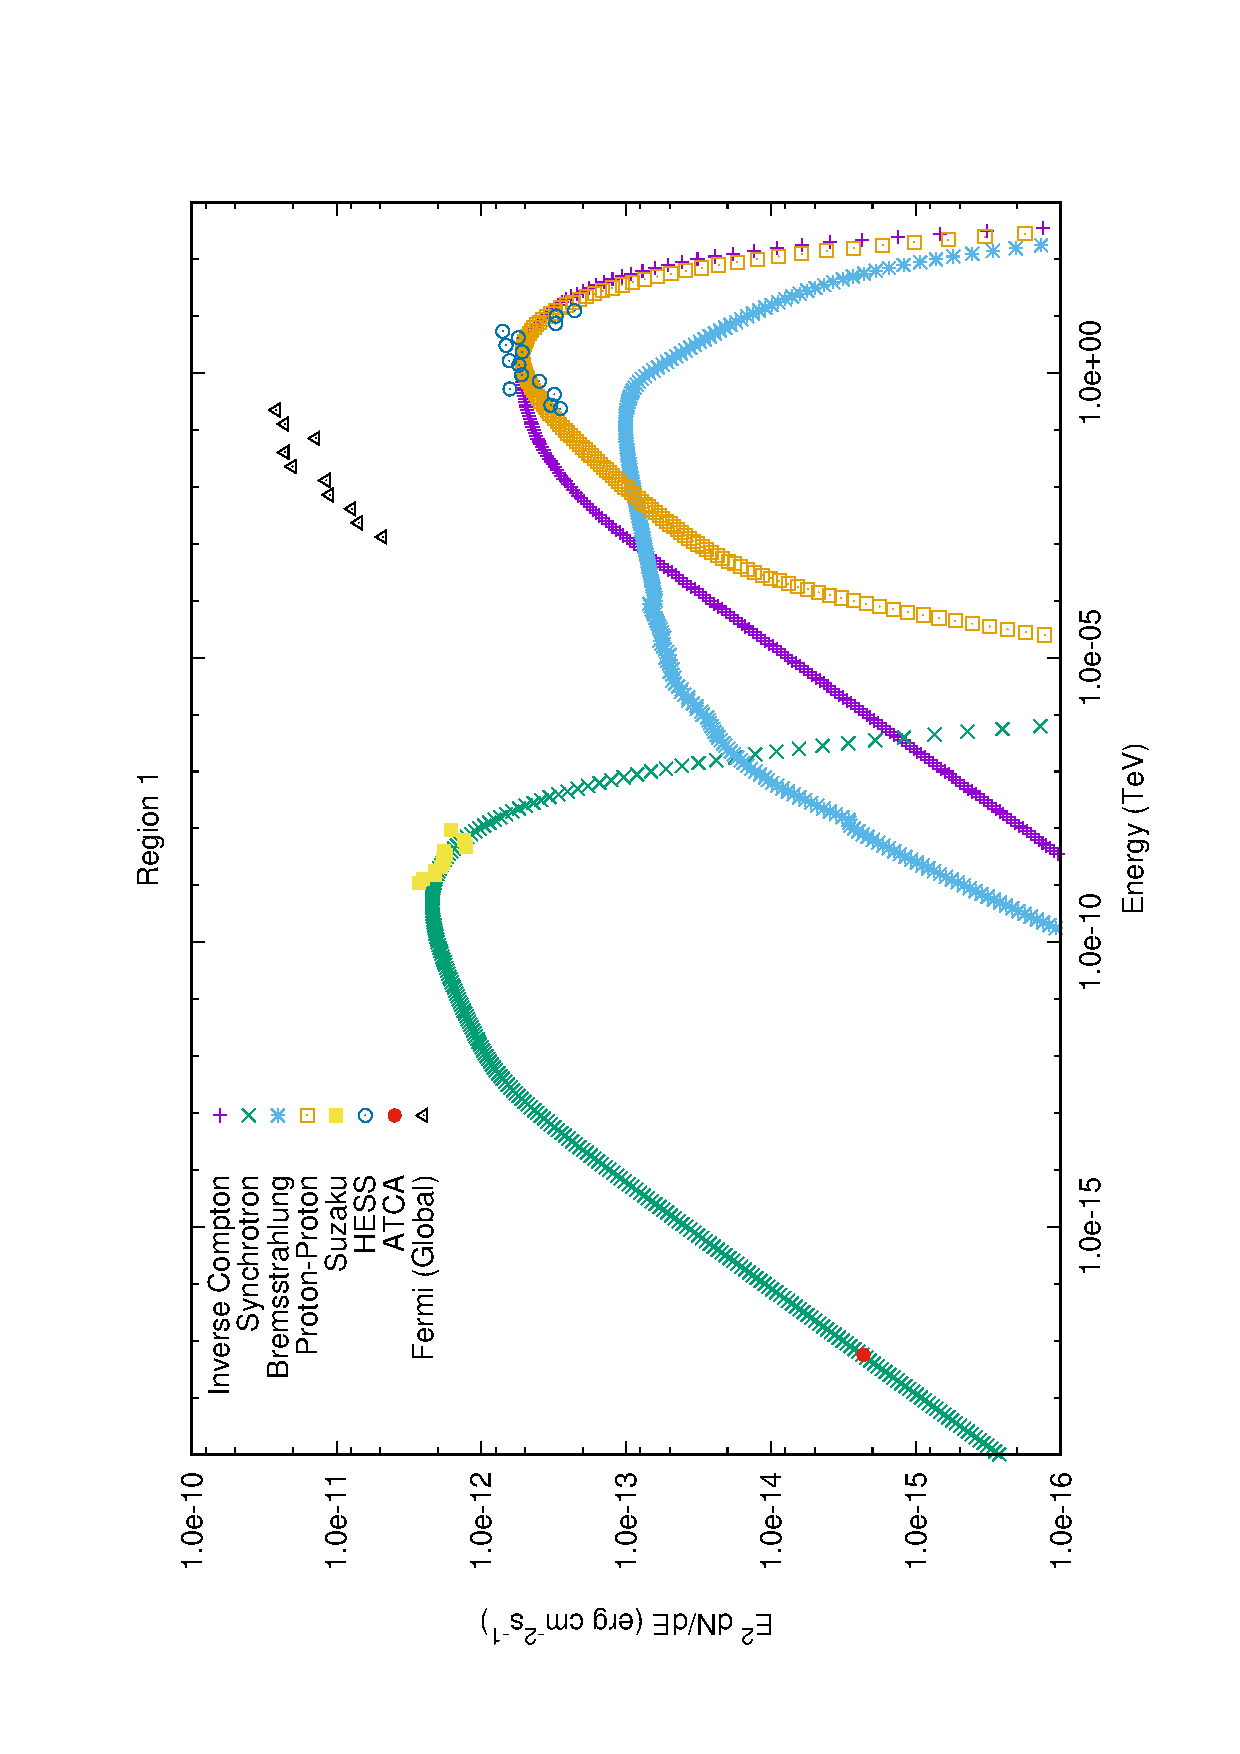
\includegraphics[width=0.7\linewidth, height=0.27\textheight, angle=-90]{rxj1713_lephad1}
		\label{fig:rxj1713lephad1}
	\end{subfigure}
	\begin{subfigure}{0.5\textwidth}
		\centering
		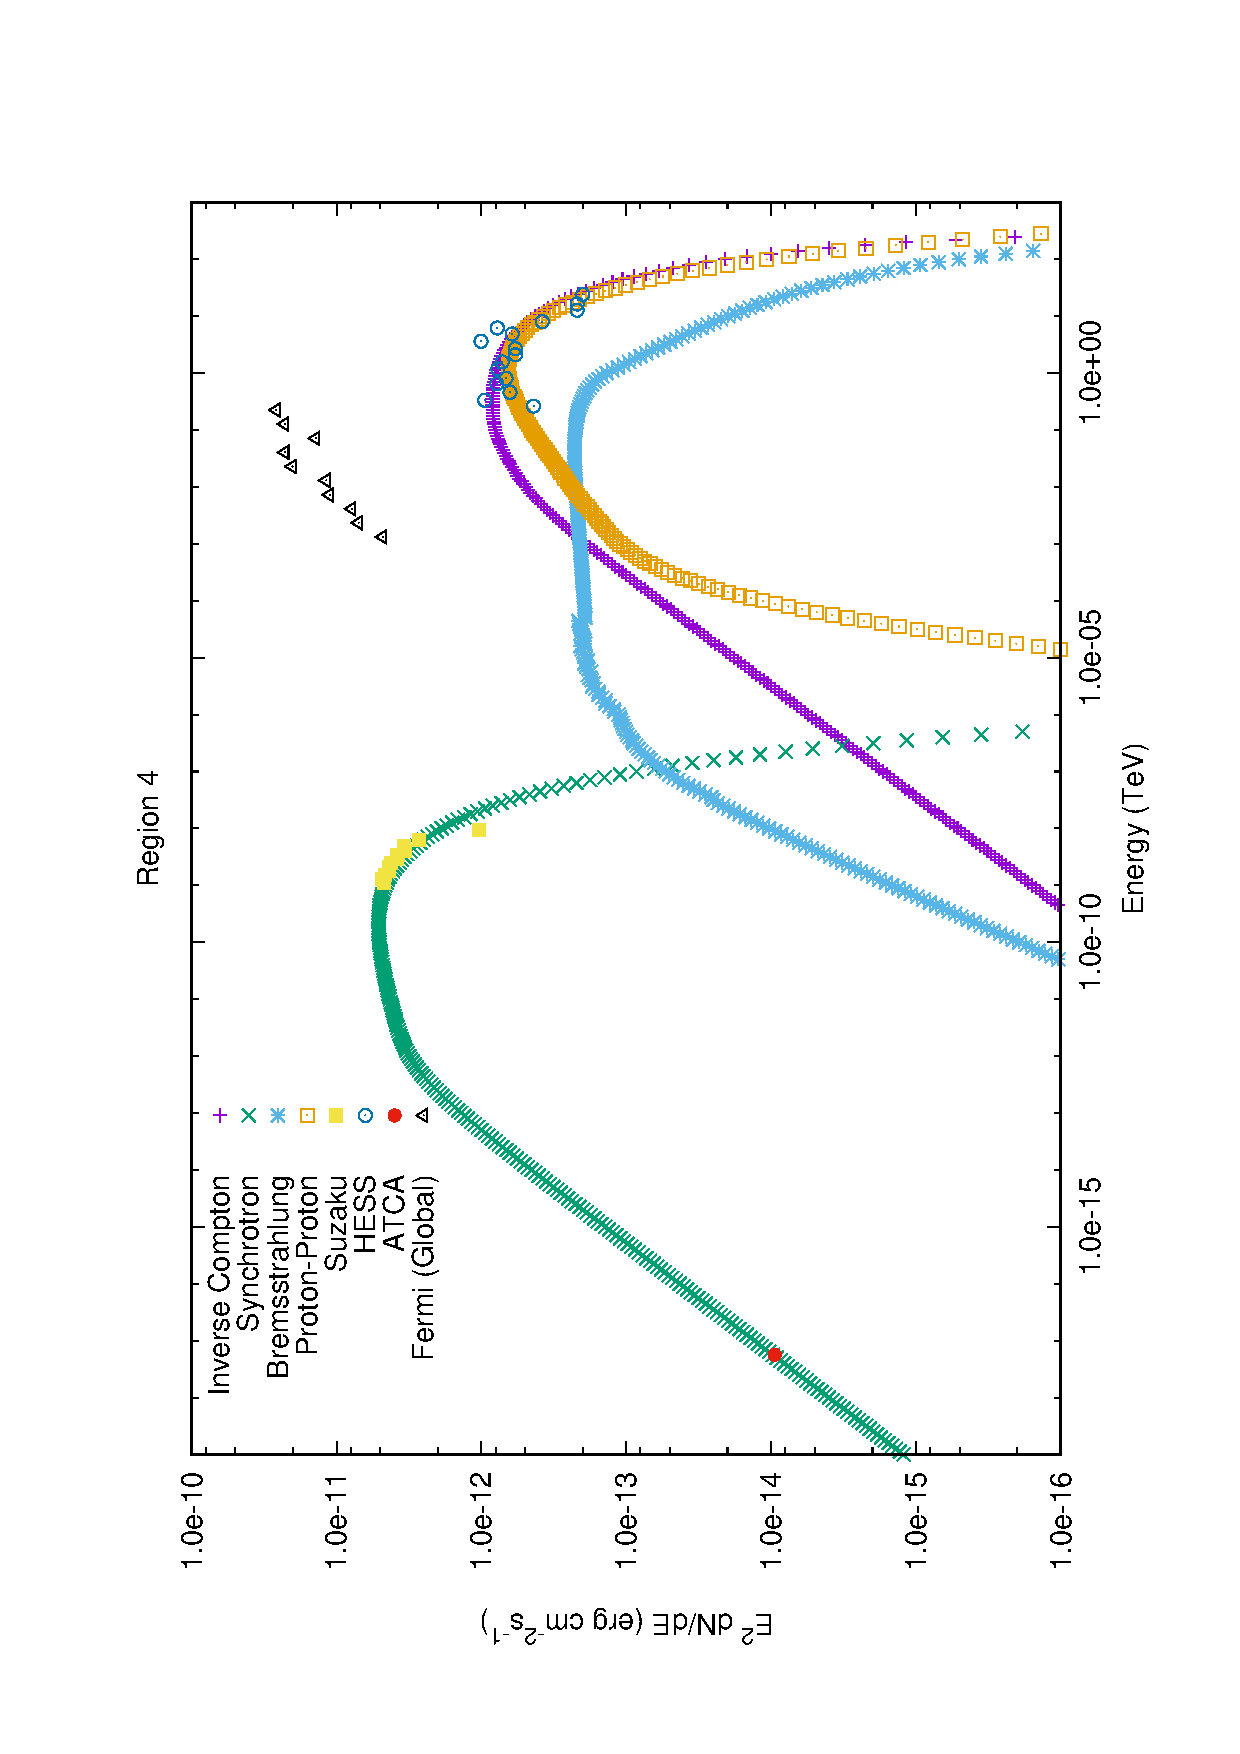
\includegraphics[width=0.7\linewidth, height=0.27\textheight, angle=-90]{rxj1713_lephad4}
		\label{fig:rxj1713lephad4}
	\end{subfigure}
	\begin{subfigure}{0.5\textwidth}
		\centering
		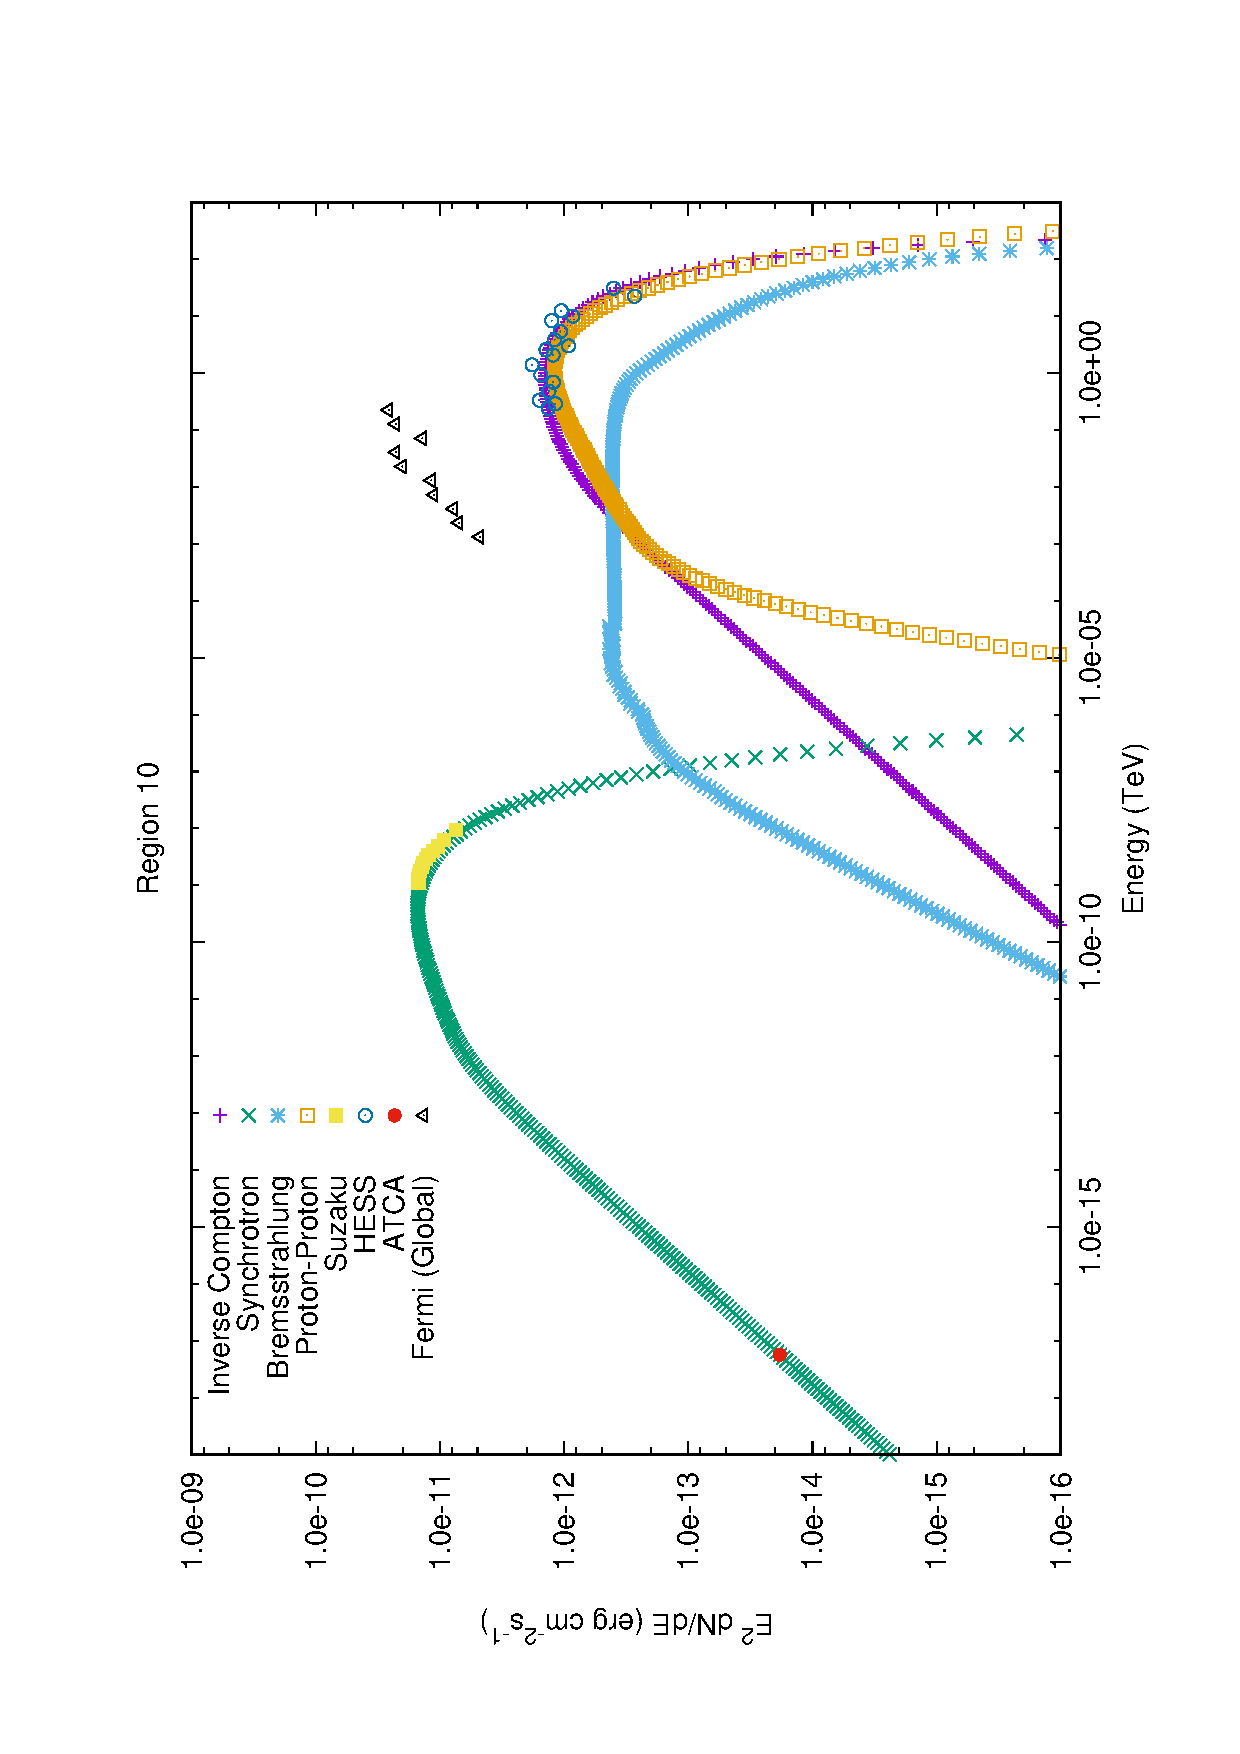
\includegraphics[width=0.7\linewidth, height=0.27\textheight, angle=-90]{rxj1713_lephad10}
		\label{fig:rxj1713lephad10}
	\end{subfigure}
	\begin{subfigure}{0.5\textwidth}
		\centering
		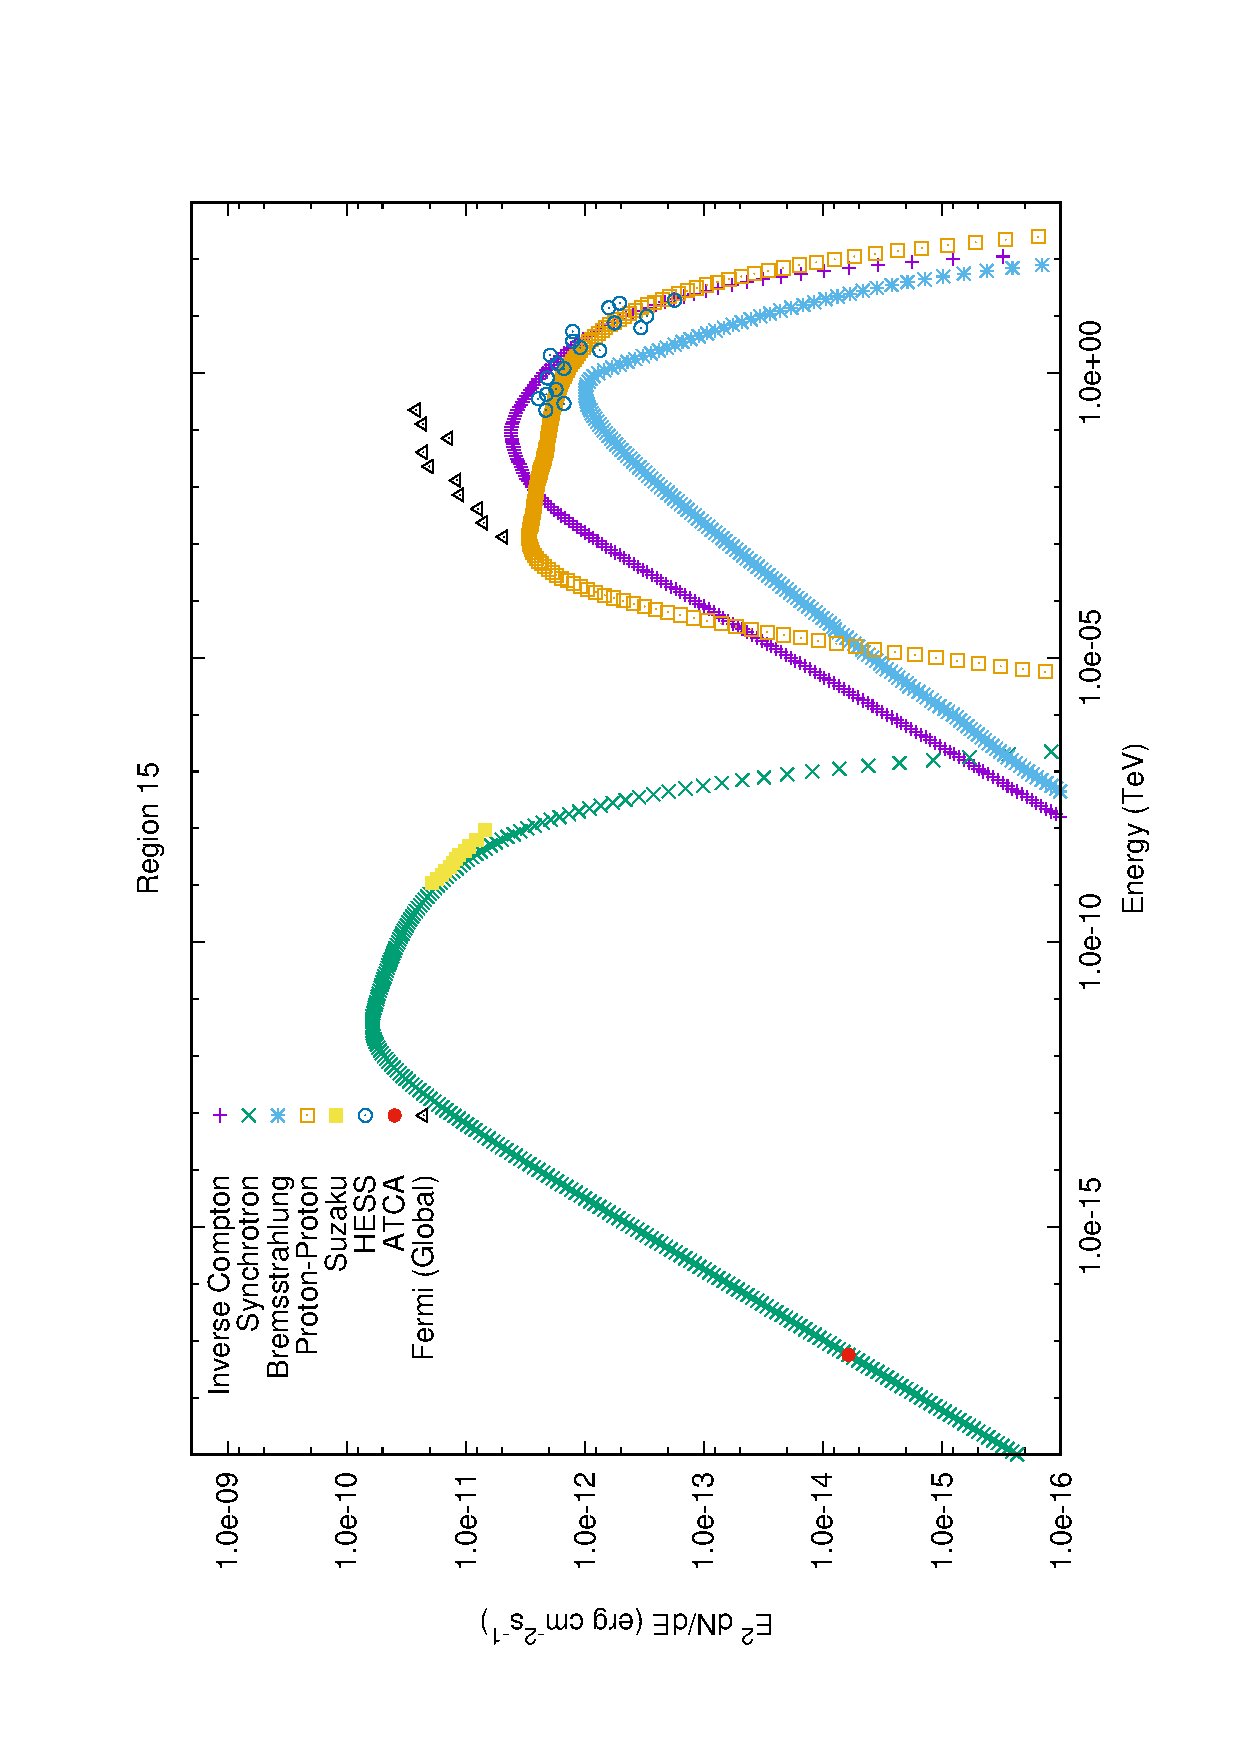
\includegraphics[width=0.7\linewidth, height=0.27\textheight, angle=-90]{rxj1713_lephad15}
		\label{fig:rxj1713lephad15}
	\end{subfigure}
	\begin{subfigure}{0.5\textwidth}
		\centering
		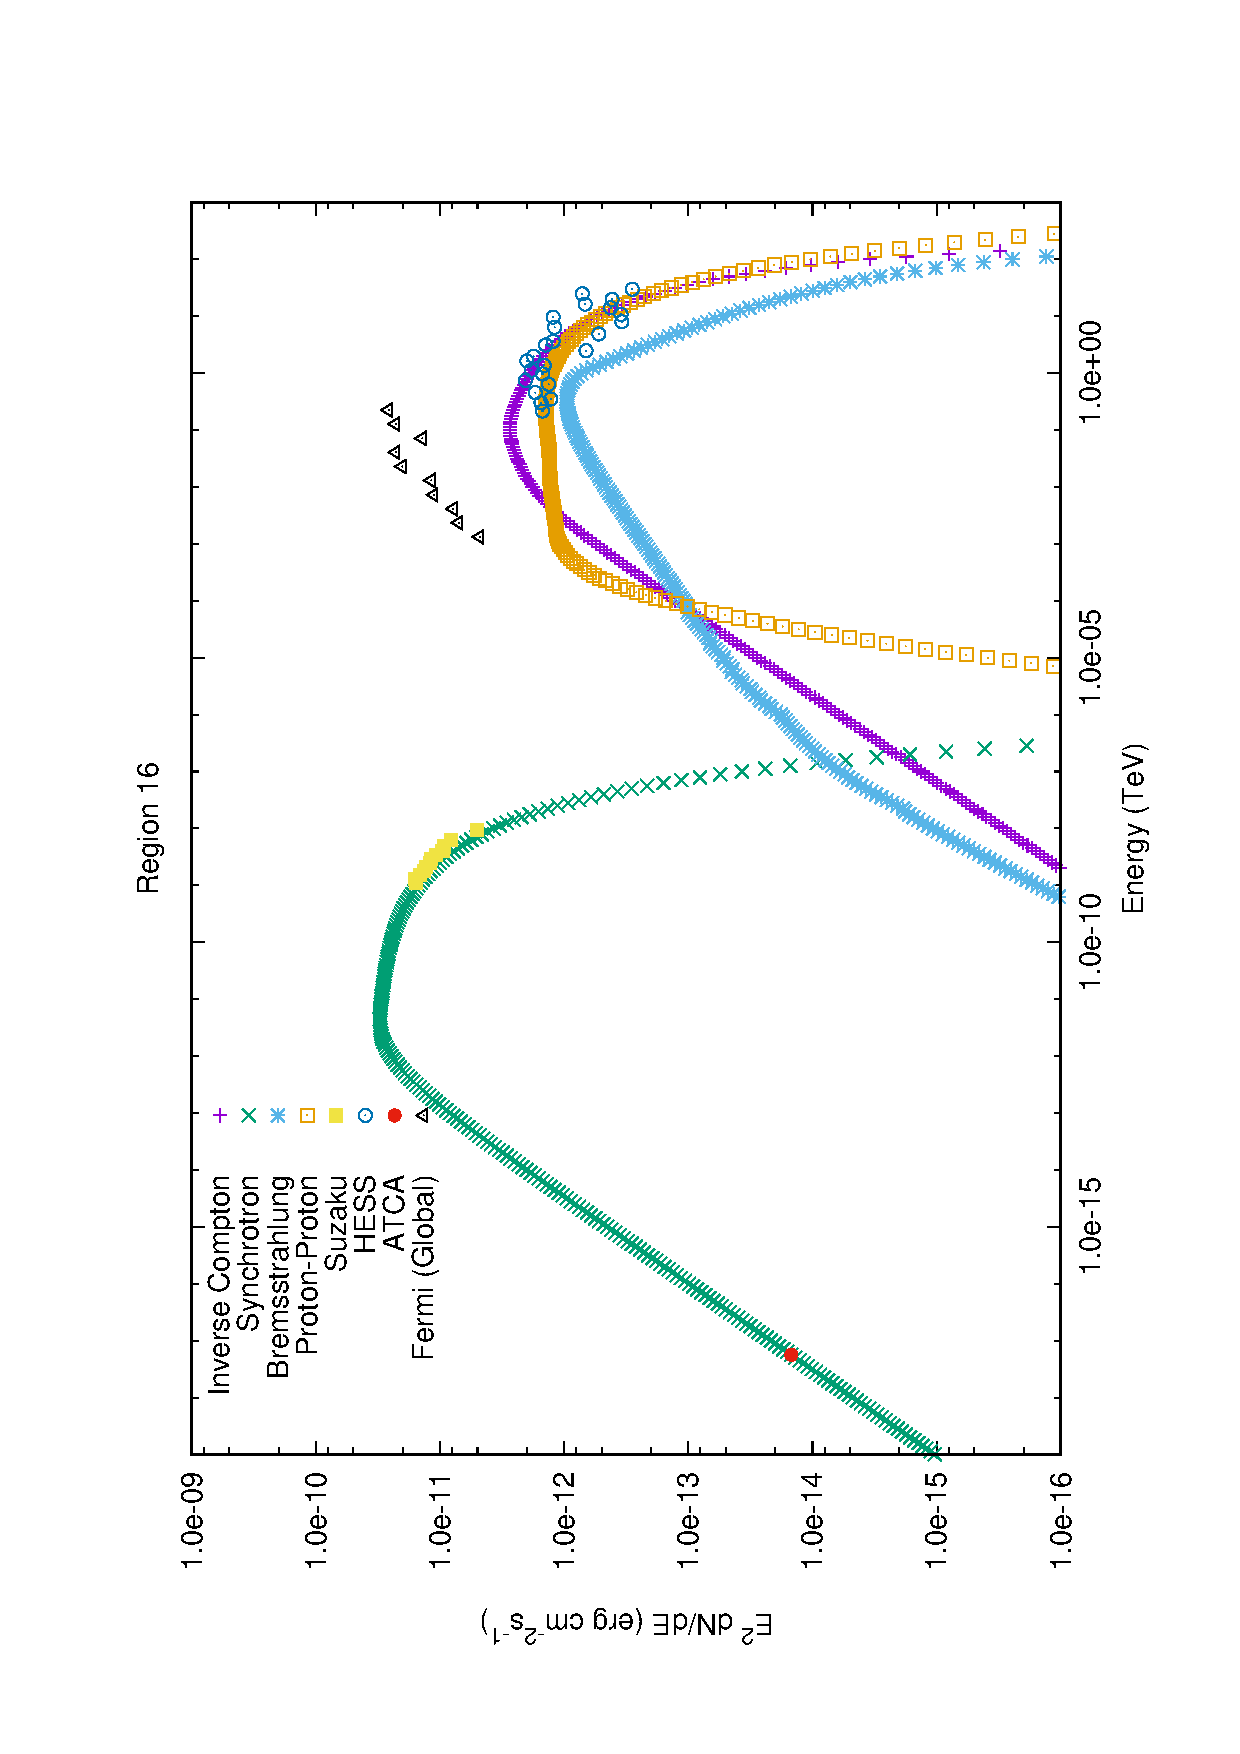
\includegraphics[width=0.7\linewidth, height=0.27\textheight, angle=-90]{rxj1713_lephad16}
		\label{fig:rxj1713lephad16}
	\end{subfigure}
	\begin{subfigure}{0.5\textwidth}
		\centering
		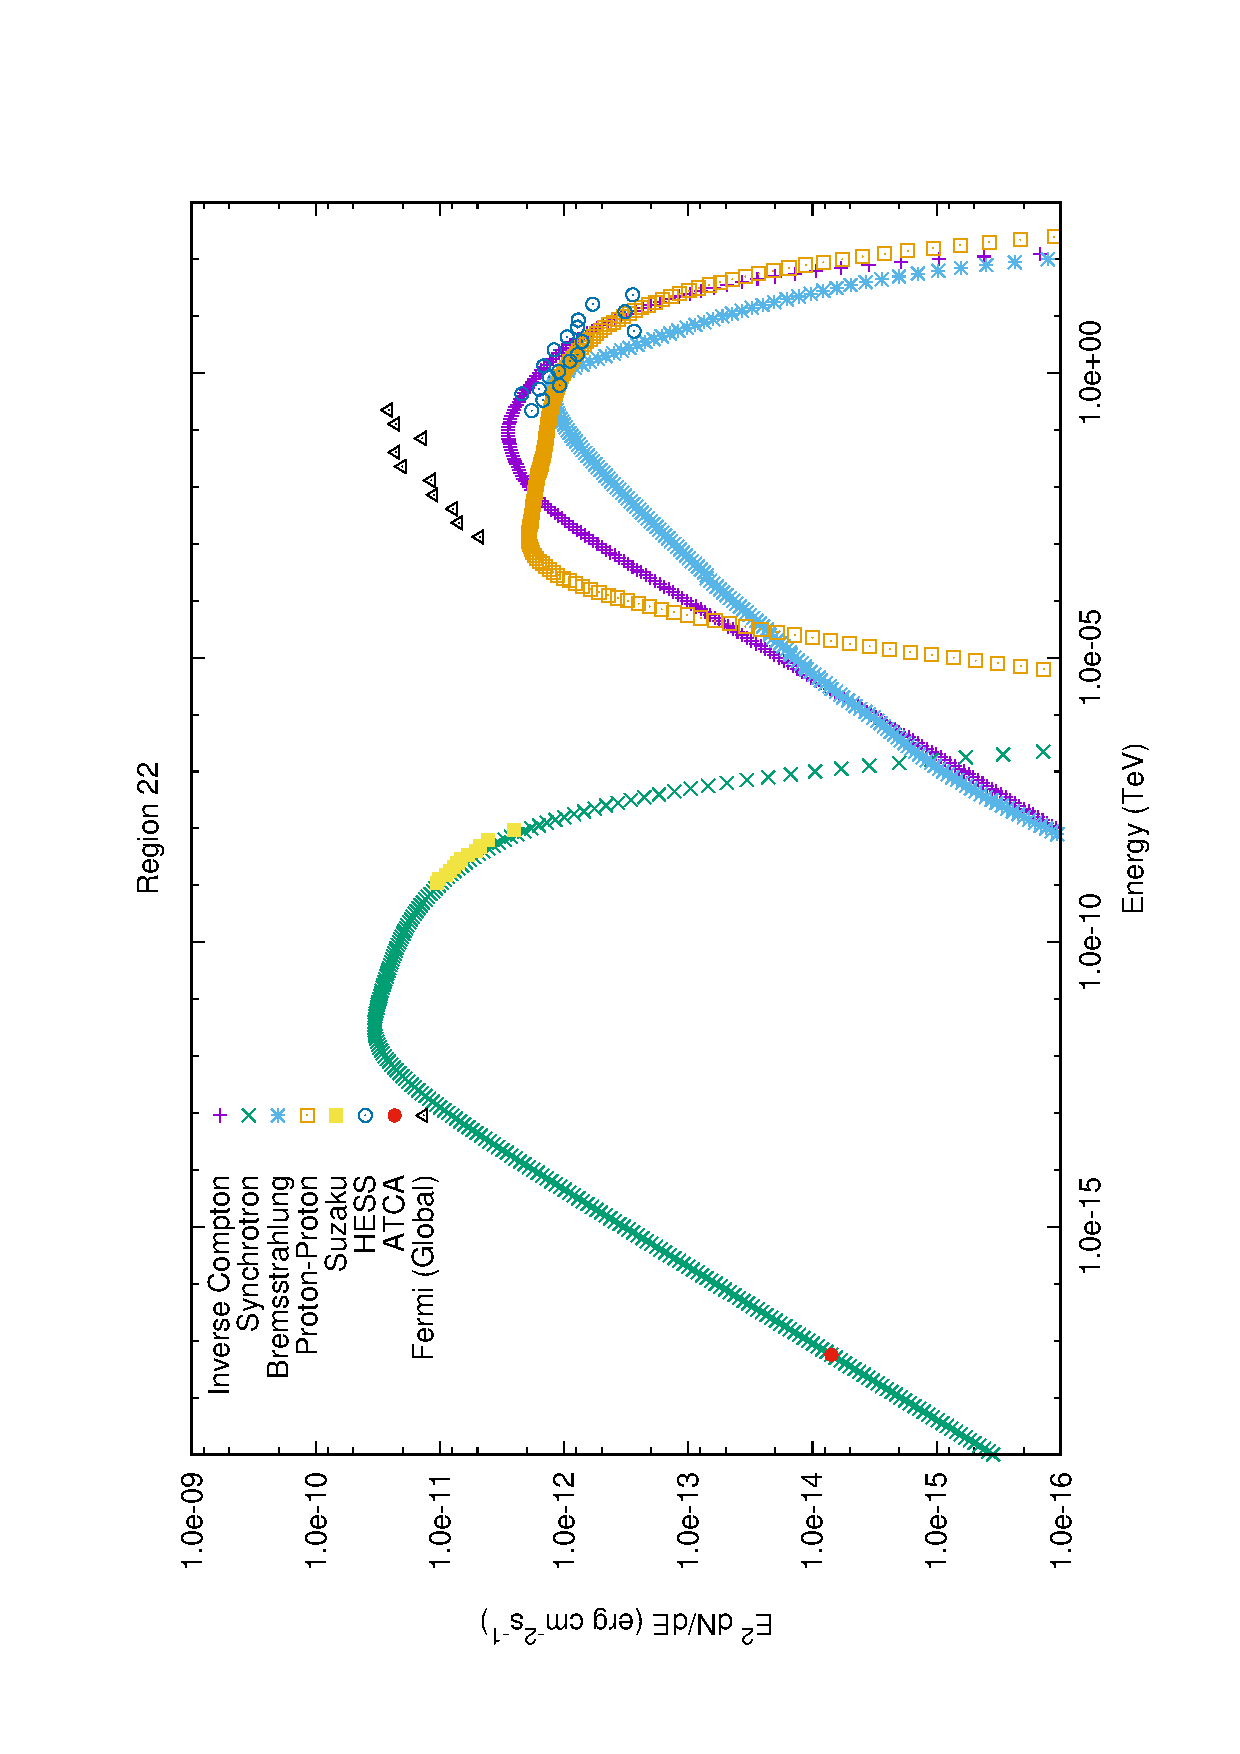
\includegraphics[width=0.7\linewidth, height=0.27\textheight, angle=-90]{rxj1713_lephad22}
		\label{fig:rxj1713lephad22}
	\end{subfigure}
	\caption{SEDs for 6 regions within RX J1713.7-3946}
	\label{fig:regionalseds}
\end{figure}

\subsubsection{Combined Modeling}
As mentioned above, a combined model of leptonic and hadronic scenarios should be investigated to help determine the nature of the particles within the SNR. A combined model would incorporate the spectra from PP, IC, Synchrotron and Bremsstrahlung processes. A slightly more hadronic scenario will be favoured if the gas is highly dense and not many X-rays are present; we would expect more CR protons to be ejected in a region like this. While a leptonic scenario will be favoured for the opposite case, a higher amount of CR electrons should be ejected from the SNR region. Additionally, the CR proton/electron ratio of 100:1 should be taken into account for the remnant as a whole. The proton fraction parameter is used to constrain the fraction of protons ejected from the SNR, assuming the only other particle is electrons. From figure 17 in \ref{2008ApJ...685..988T} we can see that X-rays are most intense around a shell like feature similar to the $\gamma$-ray flux. In figure \ref{fig:moprahesssubregions} we can see that regions to the west and north contain dense gas. Comparing both images; most sub-regions seem to have a correlation between gas density and X-rays, making it difficult to pinpoint one production scenario. It is more than likley that both hadronic and leptonic particles are being ejected so we should initialise the combined models with a proton fraction based on the 100:1 ratio. We examine multiple regions with different outstanding features to attempt to draw conclusions about the particle nature. 

Region 10 contains dense gas ($n_H$ = 156.2 cm$^{-3}$) and intense X-rays. We should expect a combined model to feature both a hadronic and leptonic contribution somewhat evenly. Hence, to fit the combined model, an initial proton fraction of 50\% was finally adapted to 59\% to fit the data. The magnetic field was also increased to B = 24.9 $\mu$G in order to fit the Synchrotron spectrum to the radio and X-ray data (figure \ref{fig:rxj1713comb10}). Additionally, the proton and electron spectrum were altered to better fit the HESS data. For the full list of parameters see table \ref{tab:regionalparamscomb}. Also of note is the large Bremsstrahlung emission at MeV energies, this is due to some parameters...
\begin{figure}[H]
	\centering
	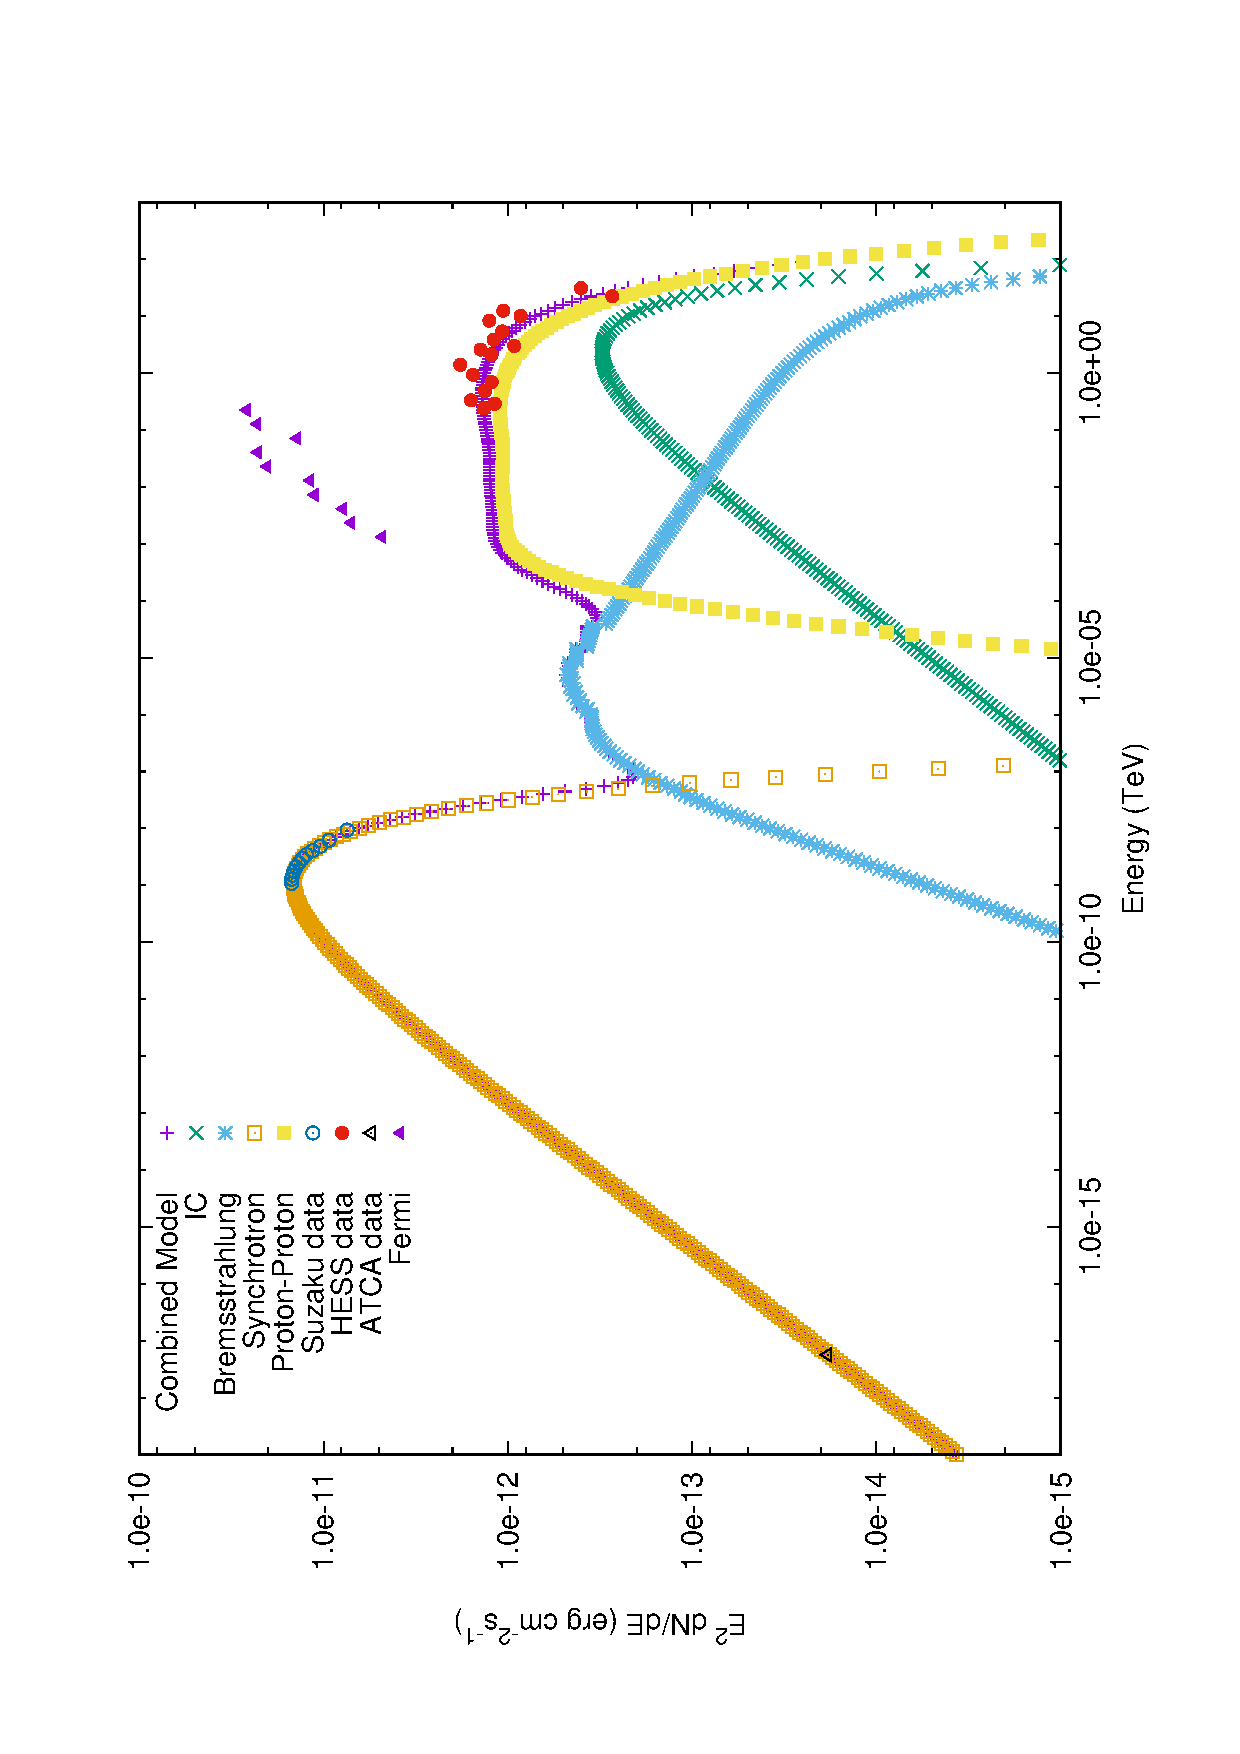
\includegraphics[width=0.4\linewidth, height=0.3\textheight, angle=-90]{rxj1713_comb10}
	\caption{SED of the combined model for region 10.}
	\label{fig:rxj1713comb10}
\end{figure}

Region 21 also contains dense gas ($n_H$ = 159.0 cm$^{-3}$) and intense X-rays. Similarly as above we begin with a proton fraction of 50\% and alter the parameters to fit the combined model to the data. The final parameter list can be found in table \ref{tab:regionalparamscomb}. A final proton fraction of 71\% fits well with the expected CR proton/electron ratio at Earth and also with the intense X-rays and dense gas. Also of note is the Bremsstrahlung spectrum at MeV energies, once again due to the parameters... (figure \ref{fig:rxj1713comb21}).
\begin{figure}[H]
	\centering
	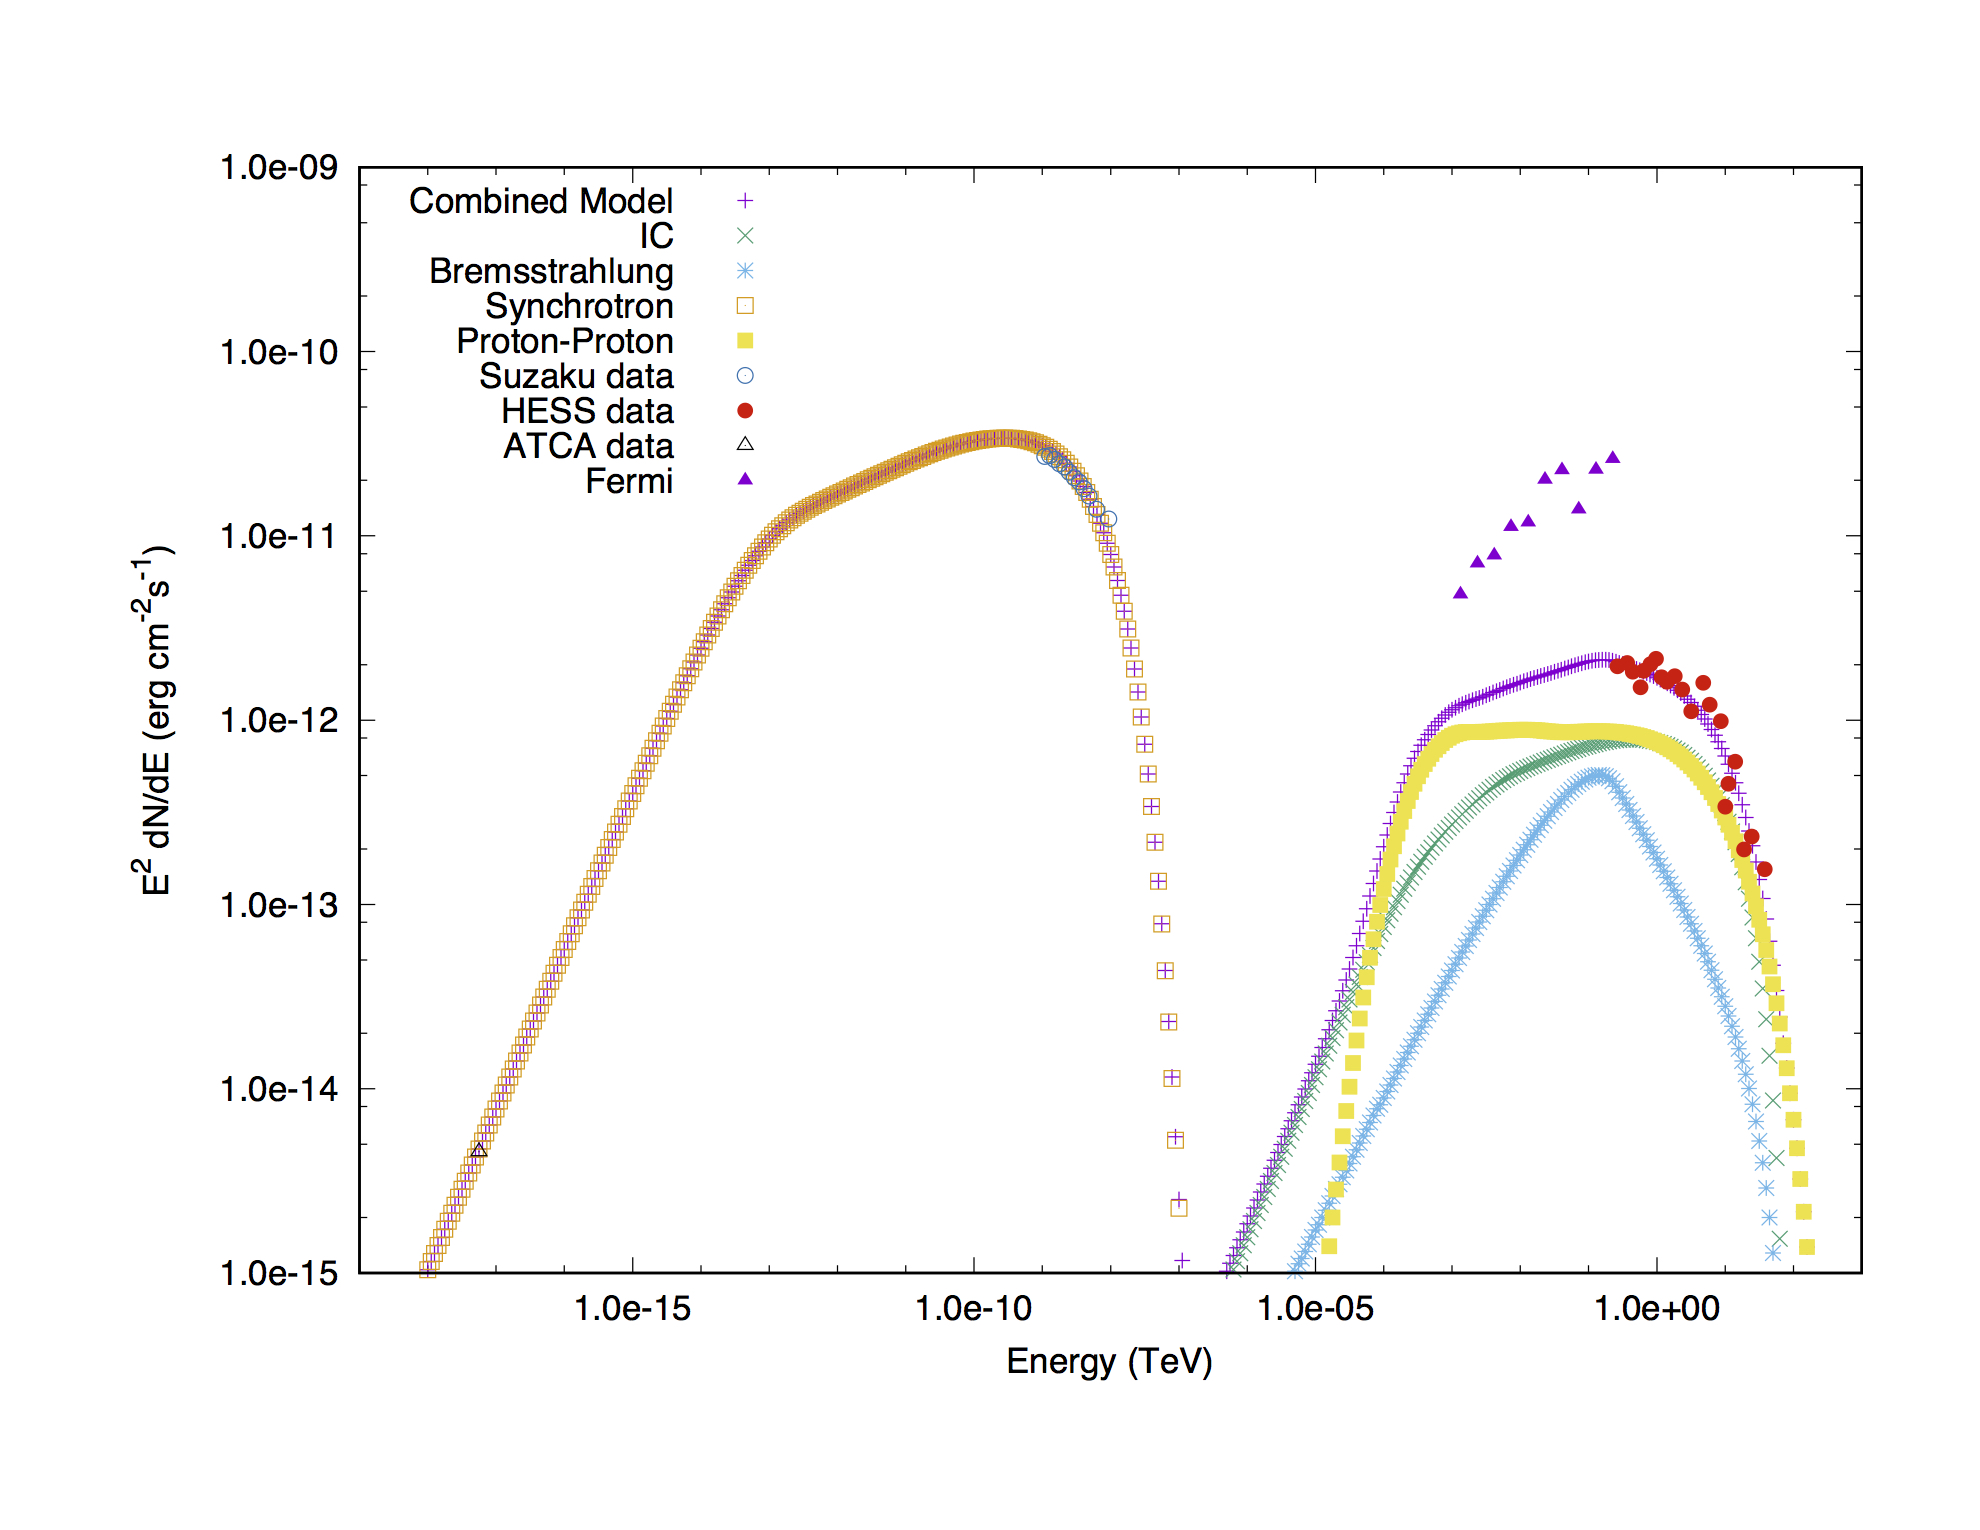
\includegraphics[width=0.4\linewidth, height=0.3\textheight, angle=-90]{rxj1713_comb21}
	\caption{SED of the combined model for region 21.}
	\label{fig:rxj1713comb21}
\end{figure}

Region 10 and 21 both display signs of a shared proton/electron population as expected. There is both dense gas, which signals the presence of hadronic interactions, and intense X-rays, which signals the presence of a Synchrotron spectrum and hence leptonic interactions. To further underestand the SNR, a region with a weak X-ray spectrum is examined (region 3). The gas density is still high in this region ($n_H$ = 142.5 cm$^{-3}$). Figure \ref{fig:rxj1713comb3} shows that the X-ray data in this region is considerably lower than the previous 2 regions, whereas the TeV emission is comparable (note the scale difference on flux axis). A high proton fraction is required to fit the combined model (95\%), which is expected. A large magnetic field is required B = 38.5 $\mu$G, but this is not unphysical if we consider the possible turbulent magnetic fields present in the shock front. The large magnetic field allows a better fit of the Synchrotron spectrum to the X-ray data and also decreases the IC spectrum allowing a large PP contribution. See table \ref{tab:regionalparamscomb} for the remaining parameters.
\begin{figure}[H]
	\centering
	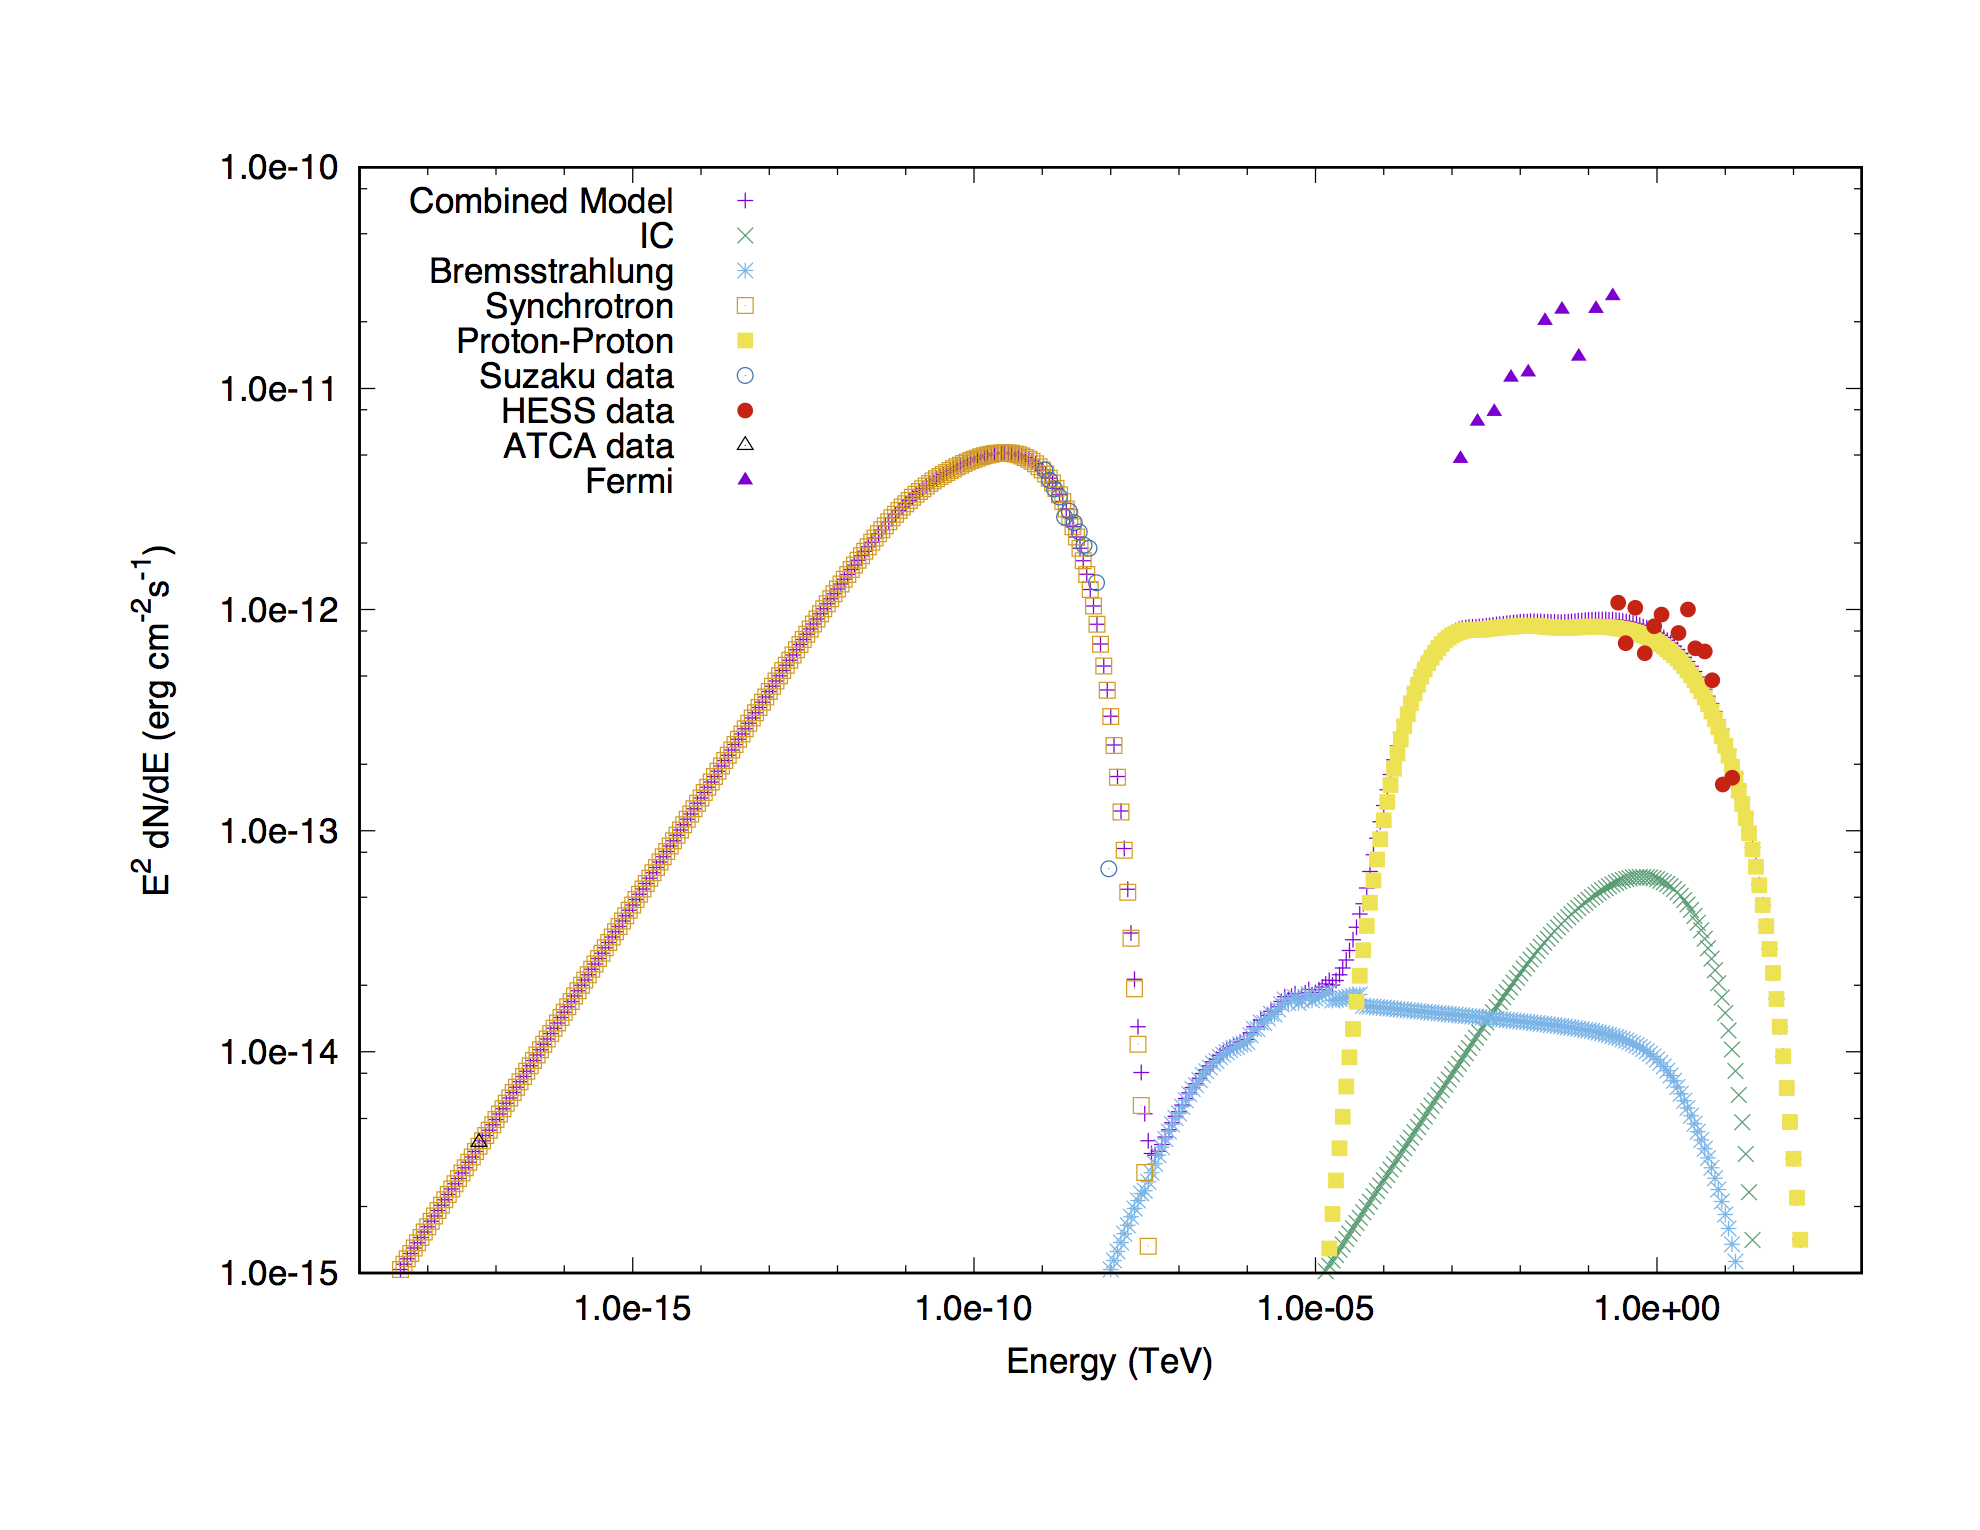
\includegraphics[width=0.4\linewidth, height=0.3\textheight, angle=-90]{rxj1713_comb3}
	\caption{SED of the combined model for region 3.}
	\label{fig:rxj1713comb3}
\end{figure}

We also examine region 22, as the Bremsstrahlung contribution at TeV energies is comparable with the IC contribution. A Bremsstrahlung contribution this large could require a very low proton fraction in order to fit all three contributions to the HESS TeV data. However, this region is the most dense region ($n_H$ = 180.7 cm$^{-3}$), with a moderate X-ray spectrum. From this point of view one would expect the proton fraction to be high. Taking in both these factors a proton fraction of 50\% is initially used. As before, this parameter and the others are changed accordingly to fit the combined model to the data. A final proton fraction of 68\% is found to make the fit (figure \ref{fig:rxj1713comb22}). The Bremsstrahlung contribution has dropped slightly, this is because so and so parameters were changed (table \ref{tab:regionalparamscomb}). One would expect the proton fraction to be greater, however, such a large Bremsstrahlung contribution indicates the presence of leptonic processes too. 
\begin{figure}[H]
	\centering
	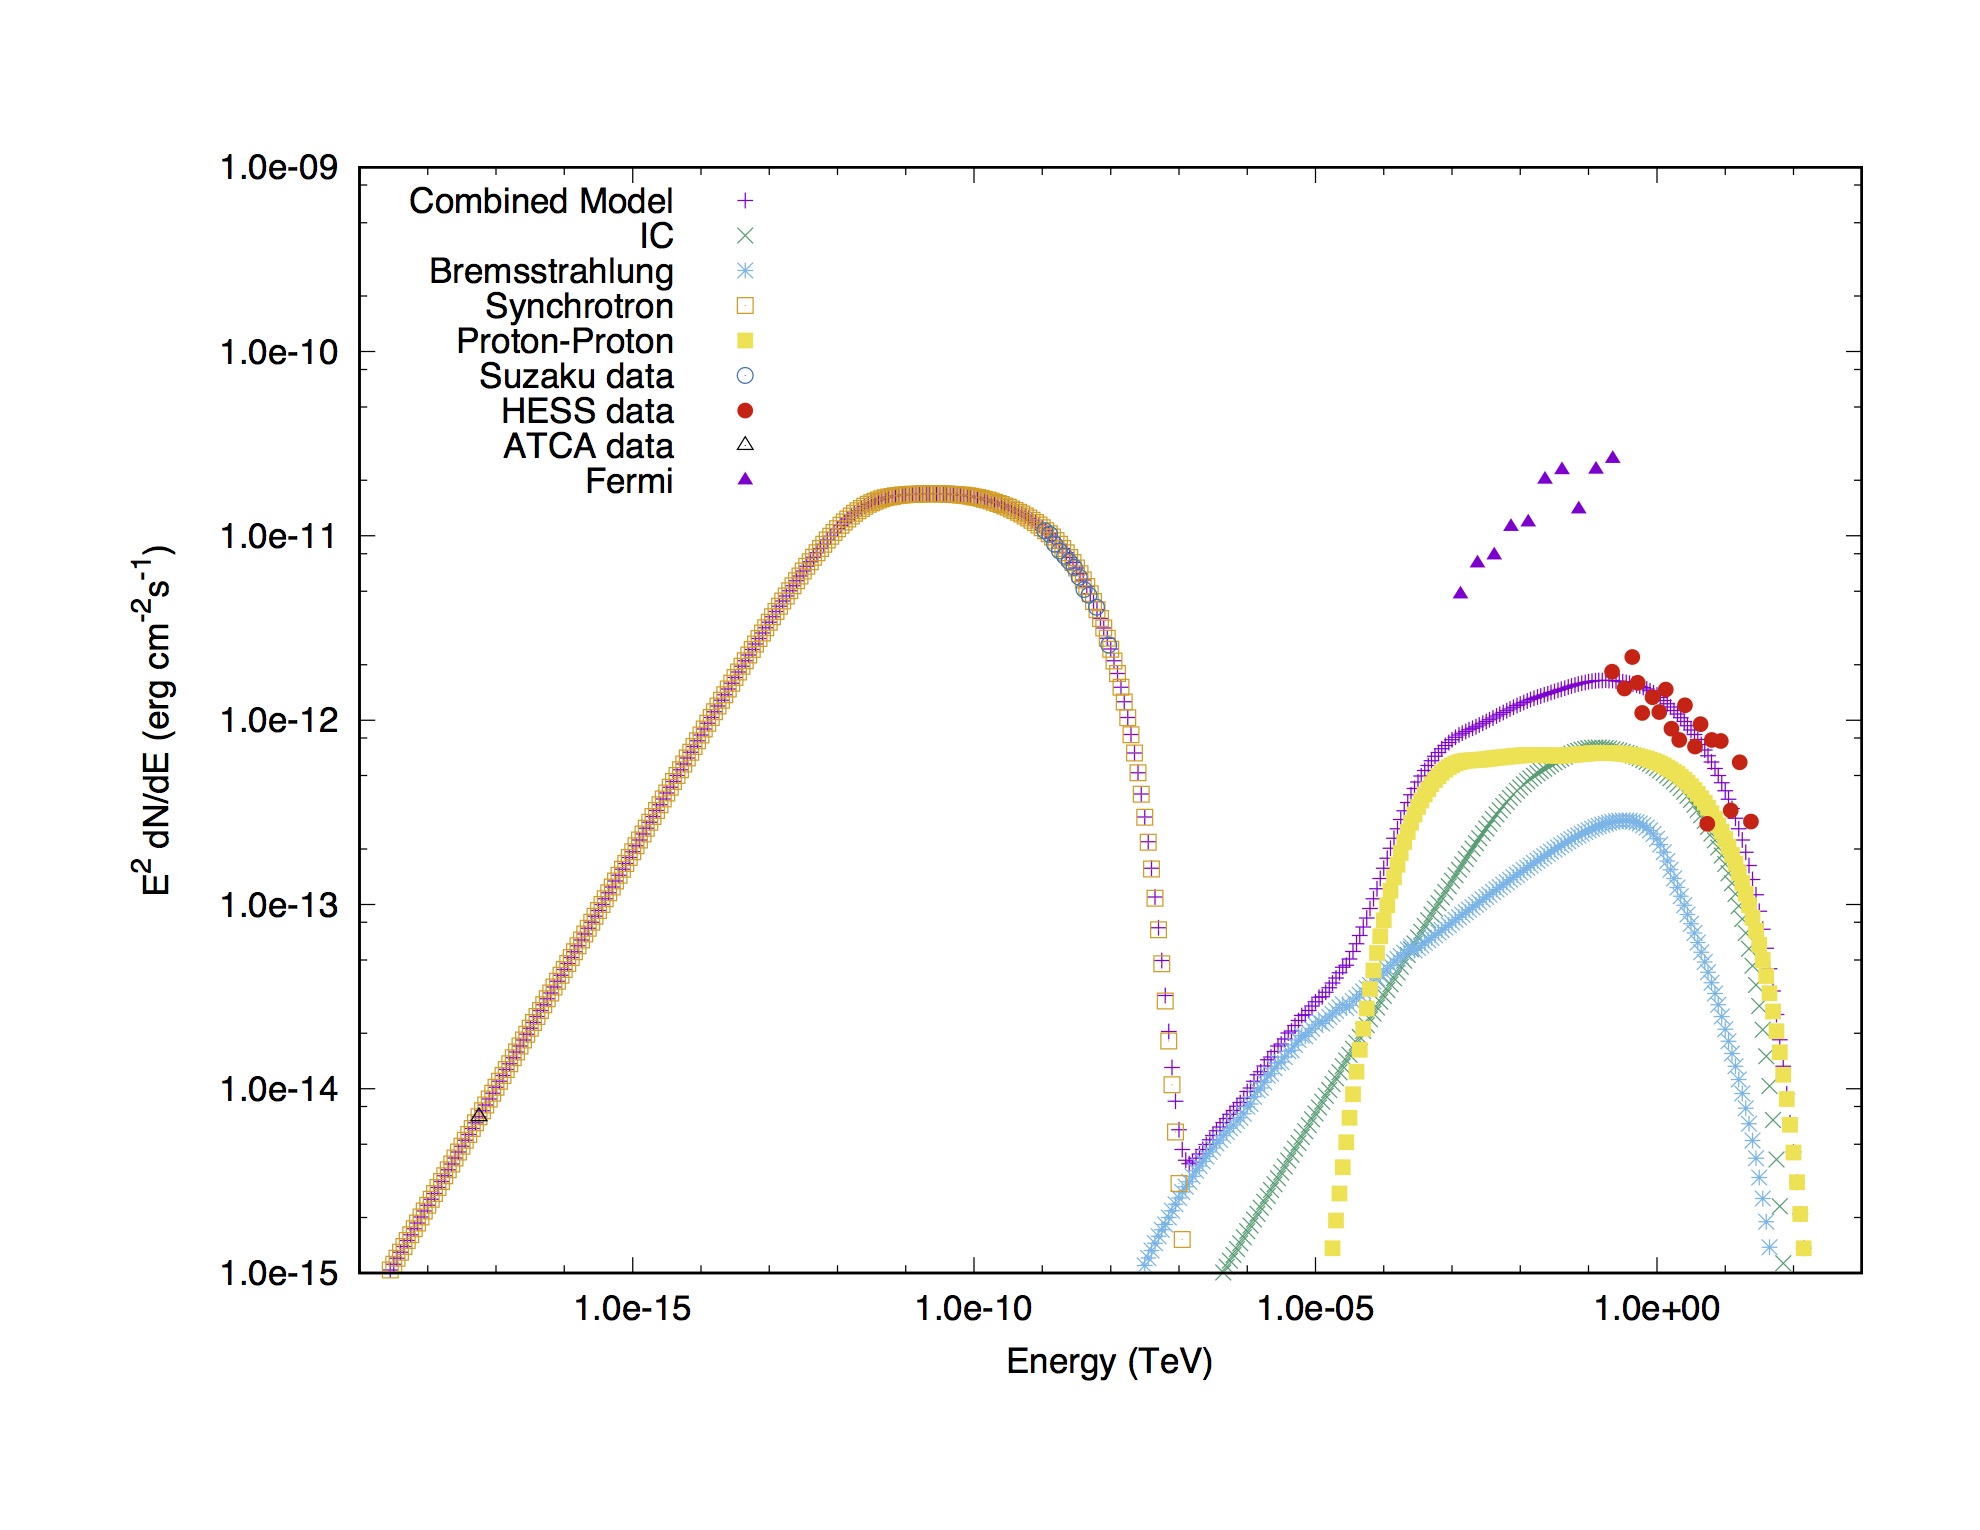
\includegraphics[width=0.4\linewidth, height=0.3\textheight, angle=-90]{rxj1713_comb22}
	\caption{SED of the combined model for region 22.}
	\label{fig:rxj1713comb22}
\end{figure}

Next, a region with less dense gas is examined. Region 7 has a density of $n_H$ = 70.01 cm$^{-3}$, while the X-ray spectrum is still moderately intense. A low proton fraction is expected for this region. Modelling as above, it is found that a proton fraction of 42\% can fit the data. Figure \ref{fig:rxj1713comb7} illustrates how IC radiation dominates the TeV part of the spectrum. A marginally lower B field is required here (B = 13.2 $\mu$G) compared to the other regions already explored, this could be an indication of a correlation between ISM gas density and magnetic field strength.  
\begin{figure}[H]
	\centering
	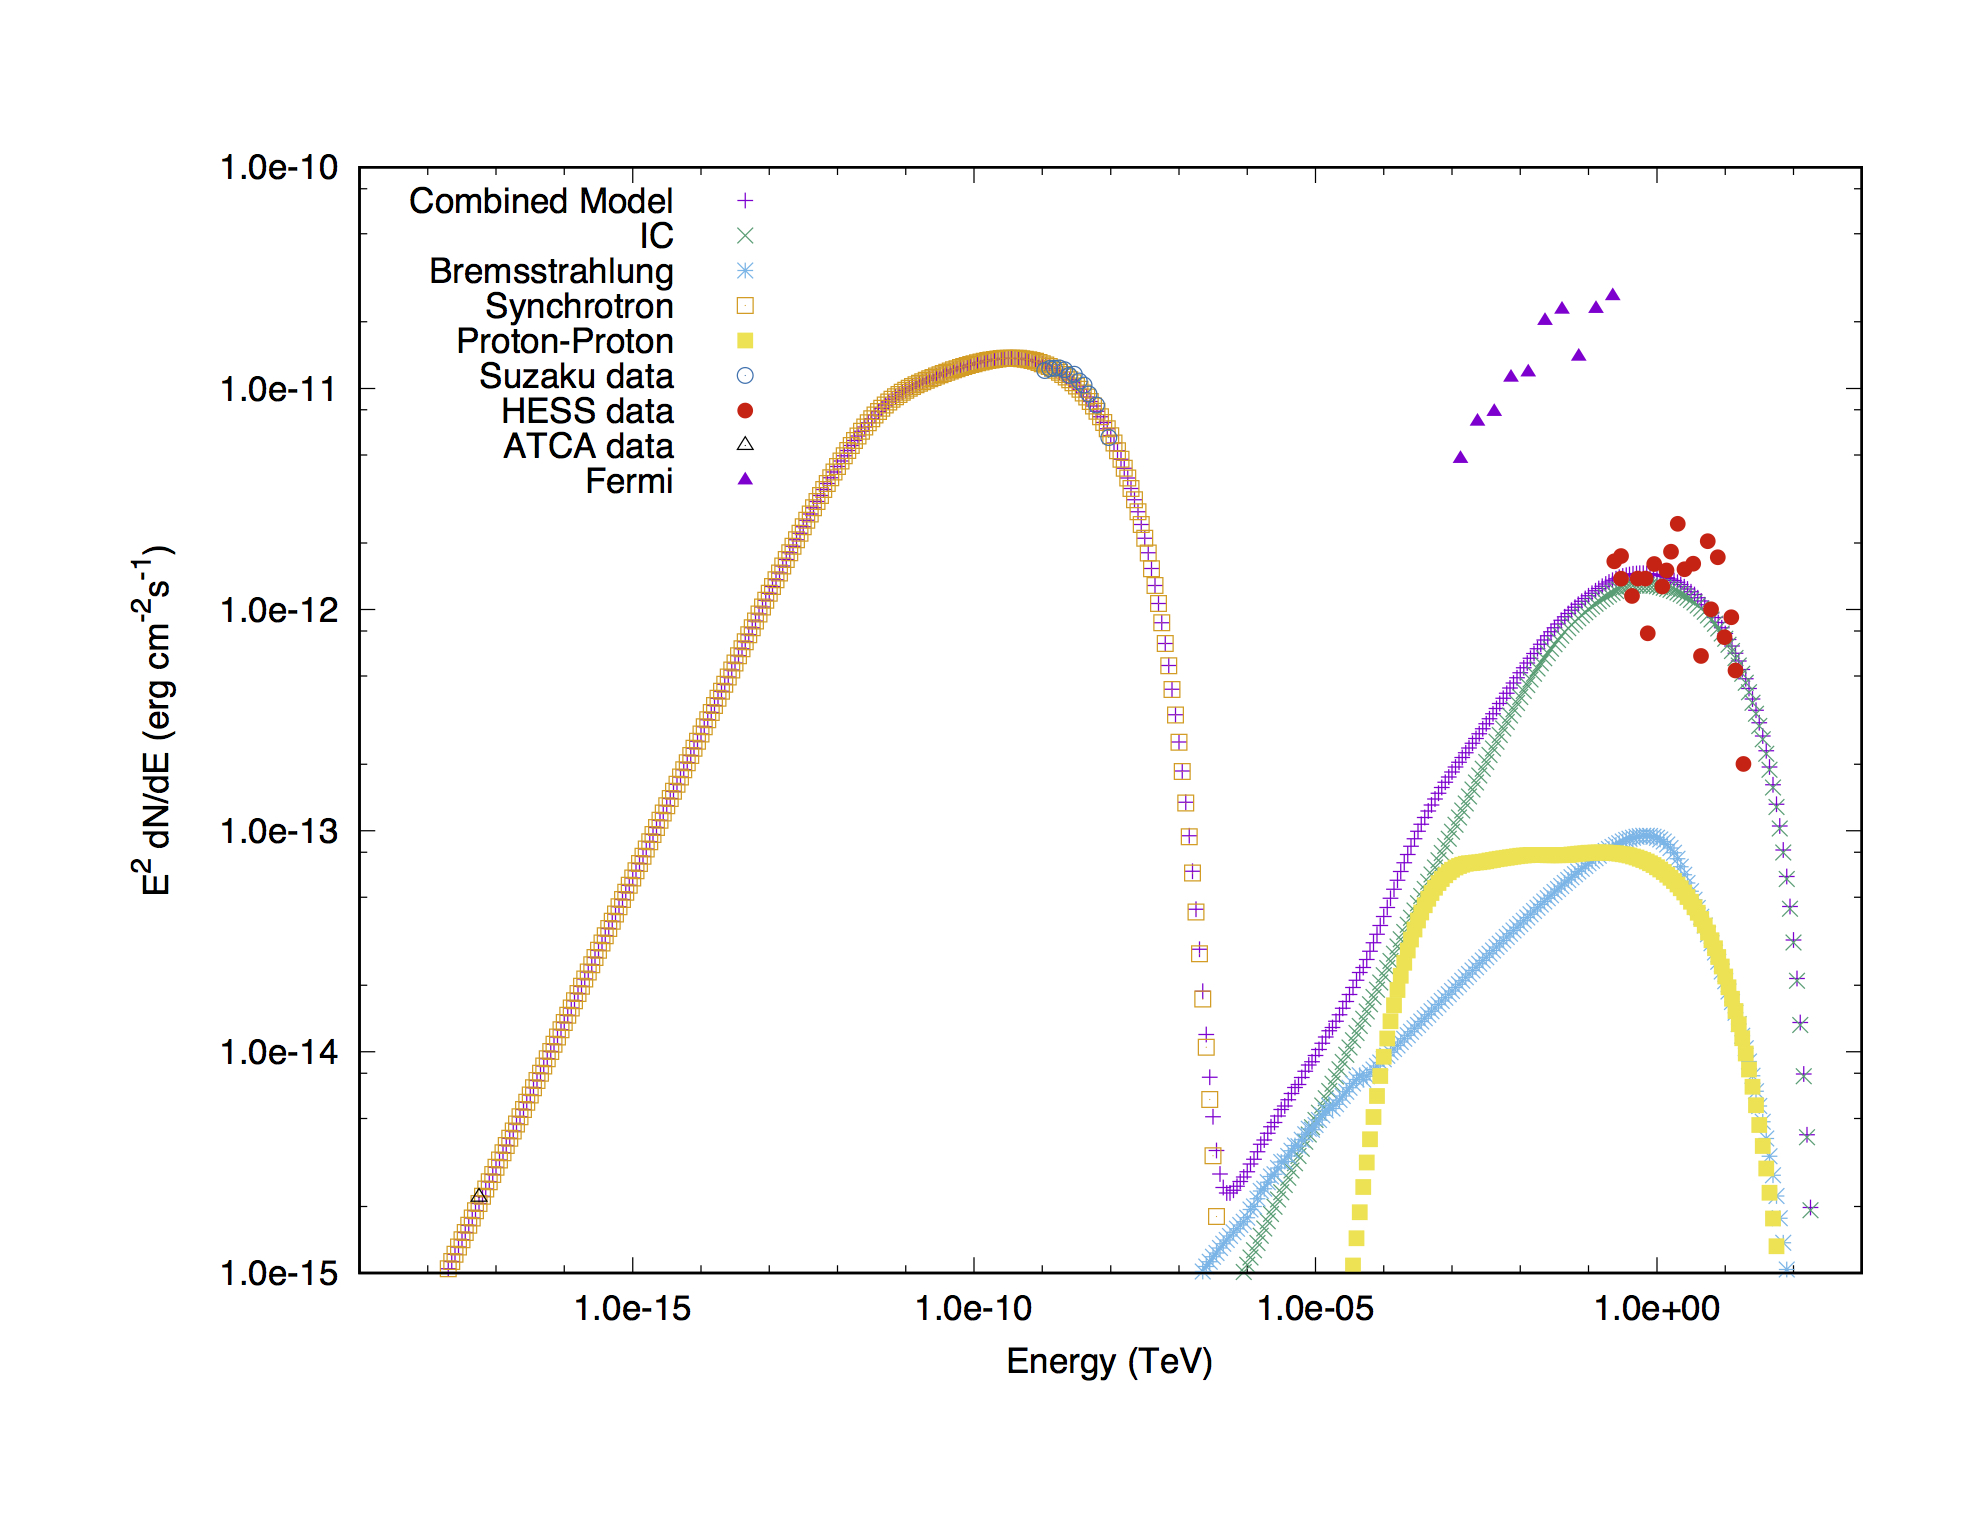
\includegraphics[width=0.4\linewidth, height=0.3\textheight, angle=-90]{rxj1713_comb7}
	\caption{SED of the combined model for region 7.}
	\label{fig:rxj1713comb7}
\end{figure}
To explore the relation between magentic field and gas density further we investigate region 18. This regions does not have an intense X-ray spectrum nor does it contain dense gas ($n_H$ = 68.27 cm$^{-3}$). A proton fraction of 92\% is required to fit the combined model to the data (figure \ref{fig:rxj1713comb18}). This is expected even though the gas has a low density, the X-ray spectrum is also low and we require more protons over the whole region to reach the expected ratio at Earth. A low magnetic field is also required (B = 17.8 $\mu$G), which strengthens the notion of gas density and magnetic field strength being related. When gas density is higher at accelerating shock fronts this could produce more intense, small-scale turbulent magnetic fields, increasing the total magnetic field for that region. 
\begin{figure}[H]
	\centering
	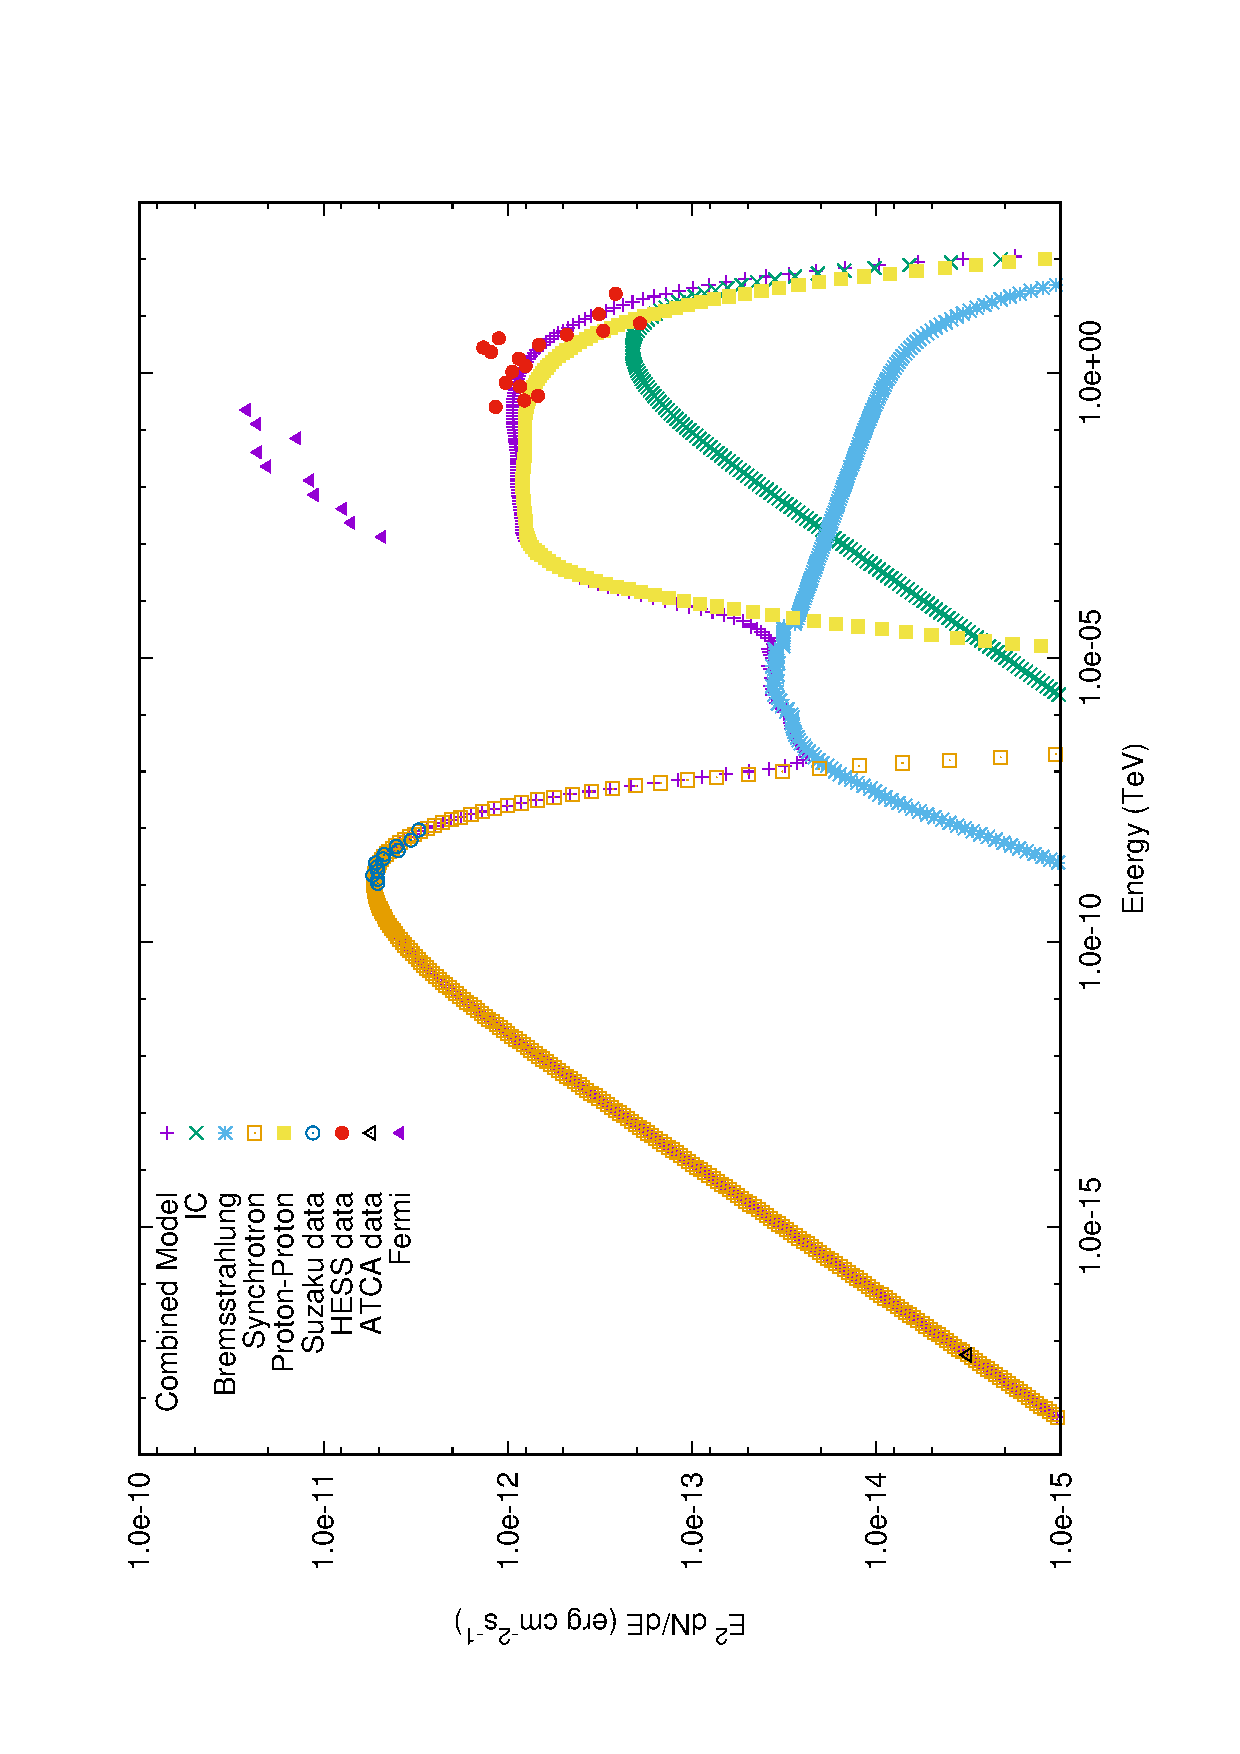
\includegraphics[width=0.4\linewidth, height=0.3\textheight, angle=-90]{rxj1713_comb18}
	\caption{SED of the combined model for region 18.}
	\label{fig:rxj1713comb18}
\end{figure}

Finally, we examine region 15. In the last chapter we saw that both the pure hadronic and pure leptonic models came remarkably close to the Fermi-LAT upper limit data. The gas in this region is moderately dense ($n_H$ = 109.6 cm$^{-3}$) and the X-ray spectrum is also moderately intense. 


Summary? It is also important to point out that the proton spectral index for all combined models is $\alpha \approx 2.04$. 
\begin{table}[H] 
	\begin{center}
		\begin{tabular}{cccccccccccc}
			\toprule 
			&
			\multicolumn{2}{c}{Shared} 
			&&
			\multicolumn{2}{c}{Proton} 
			&&
			\multicolumn{5}{c}{Electron}\\
			\cline{2-3} \cline{5-6} \cline{8-12}
			Reg.& W$_{T}$($\times 10^{46}$) & $\%_p$ && $\alpha$ & E$_c$(TeV) && B($\mu$G)&$\alpha_1$& $\alpha_2$ & E$_c$(TeV) & E$_b$(TeV)  \\
			\hline
			3 & 3.79 & 95 && 2.04 & 80 && 38.5 & 2.03 & 2.44 & 66 & 2.0\\
			7 & 1.55 & 42 && 1.94 & 71 && 13.2 & 1.69 & 2.68 & 112 & 2.2\\ 
			10 & 7.31 & 59 && 2.04 & 130 && 24.9 & 2.21 & 2.25 & 99 & 1.2\\ 
			18 & 7.94 & 92 && 2.04 & 62 && 17.8 & 2.11 & 2.25 & 80 & 5.5\\ 
			21 & 4.86 & 71 && 2.05 & 100 && 28.0 & 1.25 & 2.64 & 115 & 0.25\\ 
			22 & 3.21 & 68 && 2.03 & 93 && 23.2 & 1.72 & 2.91 & 91 & 1.2\\ 
			\bottomrule 
		\end{tabular} 
	\end{center}
	\caption{Proton and electron distribution parameters for the combined hadronic and leptonic model for each of the 29 sub-regions.}
	\label{tab:regionalparamscomb}
\end{table}


\newpage
\section{Correlation Studies of RX J1713.7-3946} \label{sec:corstudy}
In this section we examine the correlation between the ISM gas density and the HESS $\gamma$-ray flux. We begin with a simple correlation study, which categorizes regions according to their gas density and $\gamma$-ray flux. Then we proceed to perform a more quantitative study, which involves breaking each region down into smaller cells and using these smaller cells to produce a correlation factor for each region.

\subsection{Gas and \textbf{$\gamma$}-rays Correlation Analysis}
Figure \ref{fig:sgpsnantenregmaphesscont} shows the Mopra $^{12}$CO gas morphology overlaid with the $\gamma$-ray contours. The $^{12}$CO data is used as a proxy to measure the hydrogen density. So we use this map here as a quick visualisation check to see what regions are related.
\begin{figure}[h]
	\centering
	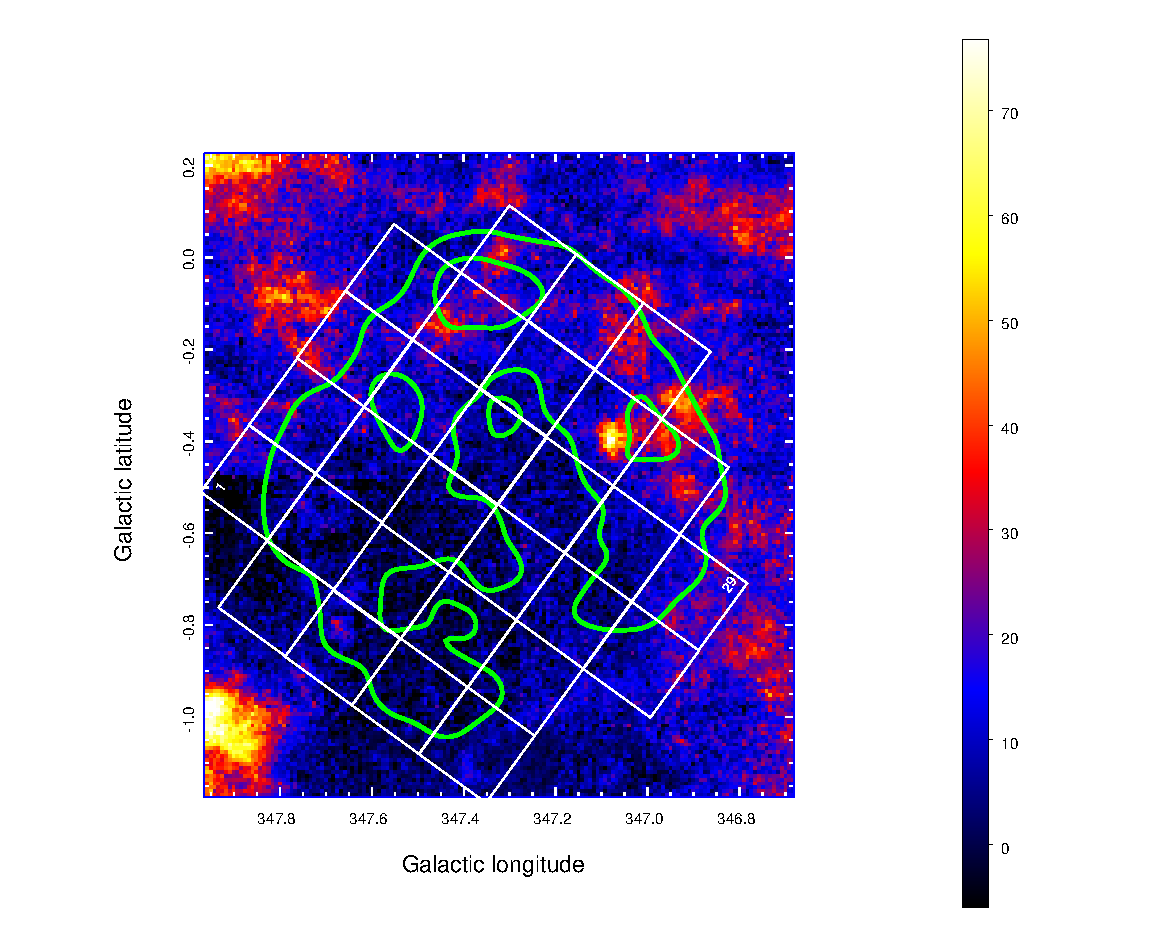
\includegraphics[width=0.75\linewidth, height=0.35\textheight]{mopra_regmap_hesscont}
	\caption{Mopra $^{12}$CO gas map overlaid with the HESS 2 TeV $\gamma$-ray contours and the 29 sub-regions.}
	\label{fig:sgpsnantenregmaphesscont}
\end{figure}
Regions along the north and following the shell around the east to the south-east appear to have some gas-$\gamma$-ray correlation. If our source is indeed a SNR shell then any potential gas that was once located near the centre of the source would've been blown away with the SNR shock front. This could be why we don't observe much gas towards the centre of our source and it forms a shell like structure, much like the $\gamma$-ray flux, around the outer regions. Table \ref{tab:densgamclass} classifies all the regions according to their ISM gas density and $\gamma$-ray flux. For $n_H < 115$, a region is defined as sparse and for $n_H > 115$ a region is defined as dense. If the total $\gamma$-ray excess counts are below 3500 then the region is considered to have a mild $\gamma$-ray flux. If the excess counts are above 5000 then the region is classified as having an intense $\gamma$-ray flux. Finally, any regions with excess counts between these two extremes are considered to have a moderate $\gamma$-ray flux. 
\begin{table}[h] 
	\begin{center}
		\begin{tabular}{c|ccc}
			\toprule
			& Mild Flux  & Moderate Flux & Intense Flux \\
			\hline
			Sparse Gas &1,5,23,24,28&2,4,11,12,13,14,15,18,19,20,25,26&6,7,8,17\\
			Dense Gas & None & 3,29 & 9,10,16,21,22,27 \\
			\bottomrule
		\end{tabular} 
	\end{center}
	\caption{Regions classified according to their ISM gas density and $\gamma$-ray flux intensity ($>$2 TeV).}
	\label{tab:densgamclass}
\end{table}
Note that no regions contain dense gas and have a mild $\gamma$-ray flux. The presence of dense gas is associated with moderate to intense $\gamma$-rays, giving us reason to believe that the gas is partly responsible for the production of these $\gamma$-rays. This supports the notion of a hadronic production scenario in these regions. Region 22 from earlier, which was shown to have a spectra that violated the Fermi-LAT observations, but also had a low $R_{\mathrm{cool/SED}}$ value, falls in this category of intense $\gamma$-rays and dense gas. It is becoming more likely that this region has a major hadronic component to its $\gamma$-ray emission, but a small leptonic contribution should not be ruled out just yet. The regions where gas is more sparse yet the $\gamma$-ray flux is still intense gives reason to believe a leptonic production scenario should be favoured. However all 4 regions with this classification have a small $R_{\mathrm{cool/SED}}$ value except for region 17. Region 17's $\gamma$-ray flux is likely leptonic in origin, whereas the other 3 require more investigation. Regions with little gas and a mild $\gamma$-ray flux may still favour a hadronic scenario, but no firm conclusions can be drawn. Similarly, no conclusions can be drawn about regions with little gas and moderate $\gamma$-rays, further investigation is required. 

\subsection{Quantitative ISM Gas Density and $\gamma$-ray Flux Correlation Analysis} \label{sec:gasgamma}
A more thorough correlation study was performed by comparing the ISM gas density with the $\gamma$-ray flux on a scatter plot. 
\subsubsection{Data Retrieval}
To correctly quantify the ISM gas density we required the total column density of both the atomic and molecular protons. The Mopra $^{12}$CO data was used as a measure for the column density of molecular protons, $N_{H_2}$, by applying an X-factor, $X$, to the observed brightness temperature, $W_M$ (equation \ref{eq:xfactor}). 
\begin{equation}
\label{eq:xfactor}
N_{H_2} = X \times W_M \ \mathrm{ cm}^{-2}
\end{equation} 
\cite{2012ApJ...746...82F} take $X$ to be $2.0 \times 10^{20}$, which we adopted in our calculations for consistency. The atomic hydrogen column density was predicted using the HI data from ATCA and the Parkes Radio Telescope \citep{2005ApJS..158..178M}. We obtained the HI column density map from \cite{2012ApJ...746...82F}, which was already converted from a brightness temperature to a column density using equation \ref{eq:HIcoldens}. As mentioned in section \ref{sec:obvs}, the velocity range is from -20 to 0 kms$^{-1}$. 

We also used the NANTEN $^{12}$CO data as a tracer for the molecular protons. The NANTEN telescope has a lower resolution than the Mopra telescope, however we expect the data to be similar. We performed the correlation study with both Mopra and NANTEN data as a tracer for molecular protons, however we used the results from Mopra as the basis for this study due to its high resolution. The analysis with the NANTEN data can be found in the appendix. We also performed a correlation study between the Mopra and NANTEN data sets to confirm they are consistent with each other (appendix).

The HESS $\gamma$-ray data were analysed in units of excess counts (as above). Each pixel in the HESS ($>$ 2 TeV) $\gamma$-ray image was smoothed and integrated over a circle of radius 0.03$^o$ (H16) to obtain the excess count number. Since the pixel size was much smaller than this, neighboring pixels will contain overlapping information. Each region has size 0.18$^o$ by 0.18$^o$ and hence contained 9 pixels with independent information. We used these 9 pixels for our correlation study to ensure we obtained a data set of independent measurements, using any more pixels didn't provide any new information. We used the Miriad software \citep{1995ASPC...77..433S} to re-bin the HESS $\gamma$-ray image into pixels with size 0.06$^o$ by 0.06$^o$, to ensure that each region contains the required 9 independent pixels (figure \ref{fig:moprahess9pixels}, top left). The re-binning functions took the average of the original, smaller pixels and used this as the new pixel value. 

We then used Miriad again to re-grid and match the Mopra $^{12}$CO map to the HESS map, so the pixels in both images were aligned (figure \ref{fig:moprahess9pixels}, top right).
In doing so, 51 pixels in the original Mopra map were averaged to obtain a total brightness temperature for each new pixel. However, for our brightness temperature values to be correct we needed to sum over these pixels, not average. We multiplied our data by a factor of 51 to account for this. We did the same with the HI column density and then combined the two maps together to obtain a total proton column density value for each pixel. The molecular column density was also multiplied by a factor of 2 to account for both protons within the H$_2$ molecule. 
\begin{figure}[H]
	\begin{subfigure}{0.5\textwidth}
		\centering
		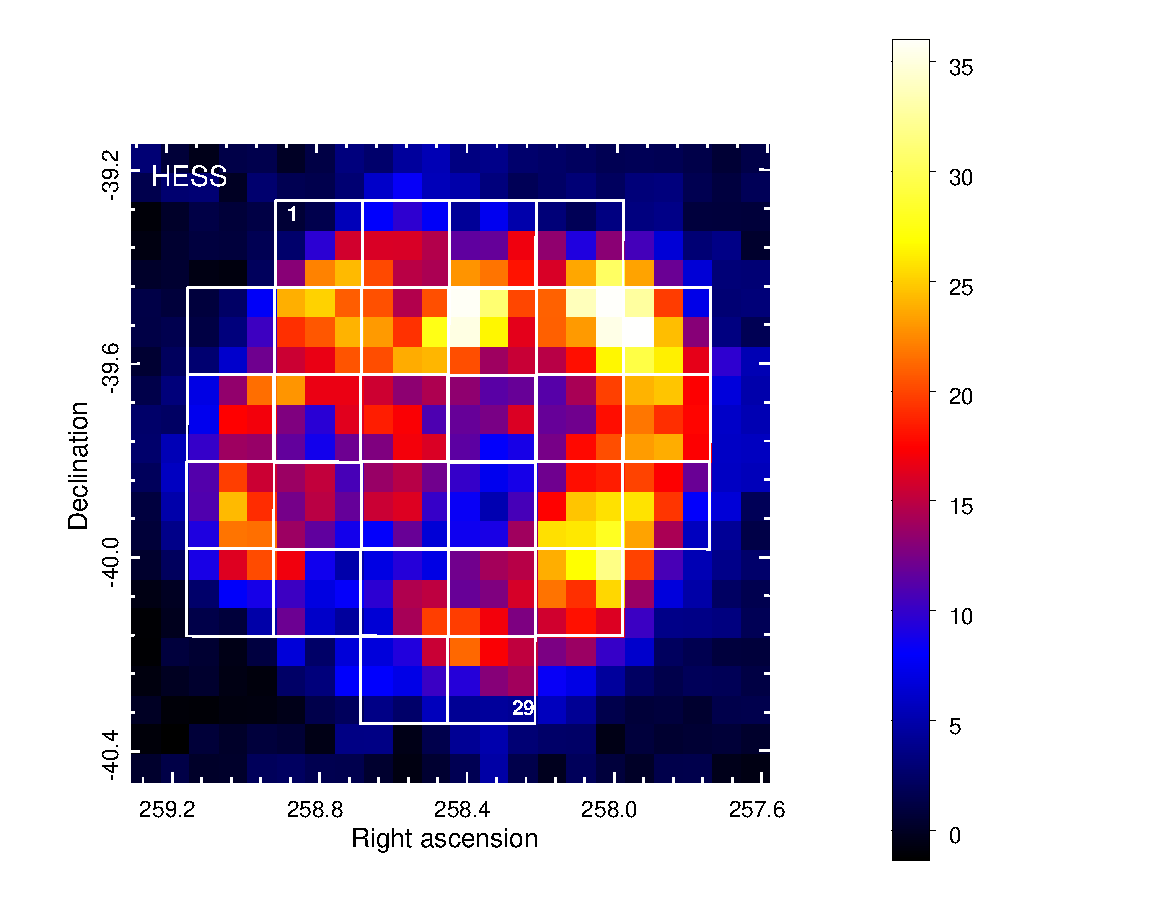
\includegraphics[width=1.05\linewidth, height=0.25\textheight]{hess_9pixels}
	\end{subfigure}
	\begin{subfigure}{0.5\textwidth}
		\centering
		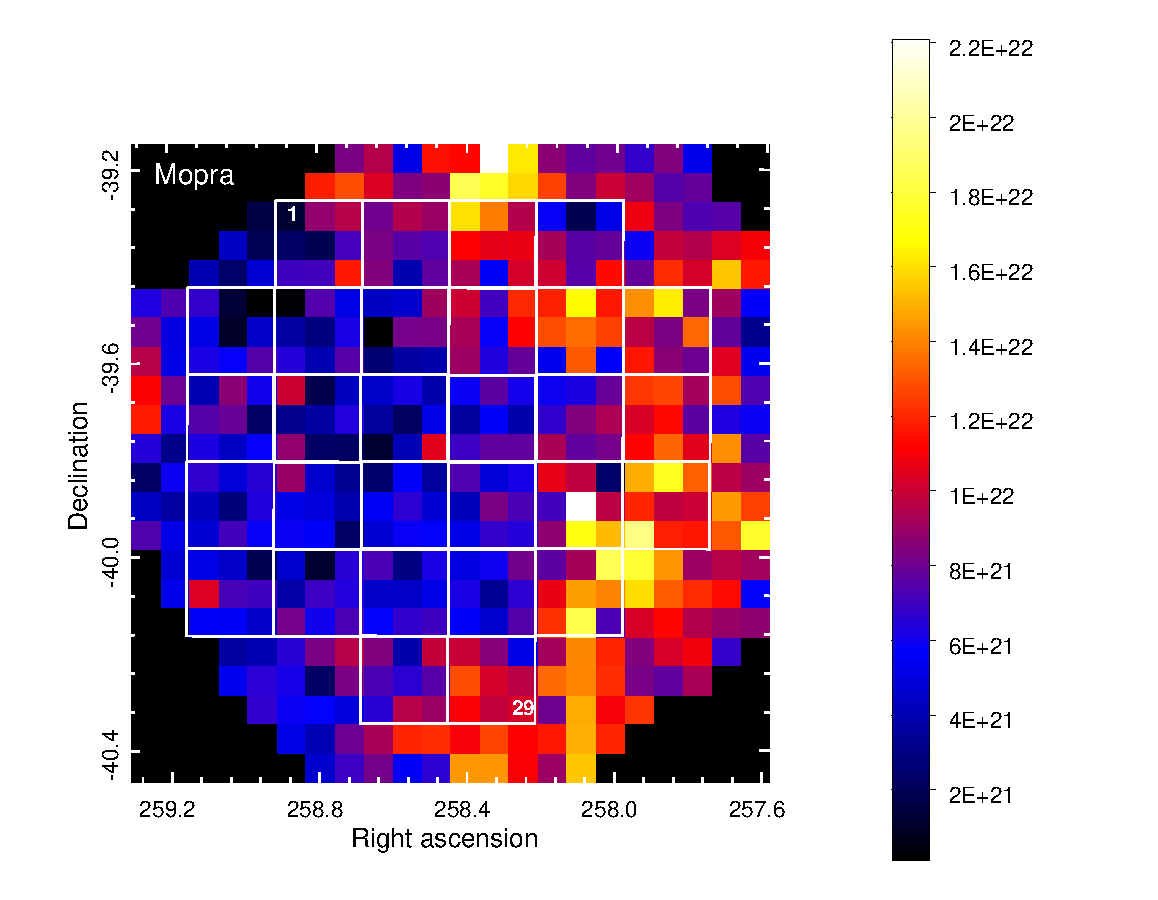
\includegraphics[width=1.05\linewidth, height=0.25\textheight]{mopra_9pixels}
	\end{subfigure}
	\begin{subfigure}{0.5\textwidth}
		\centering
		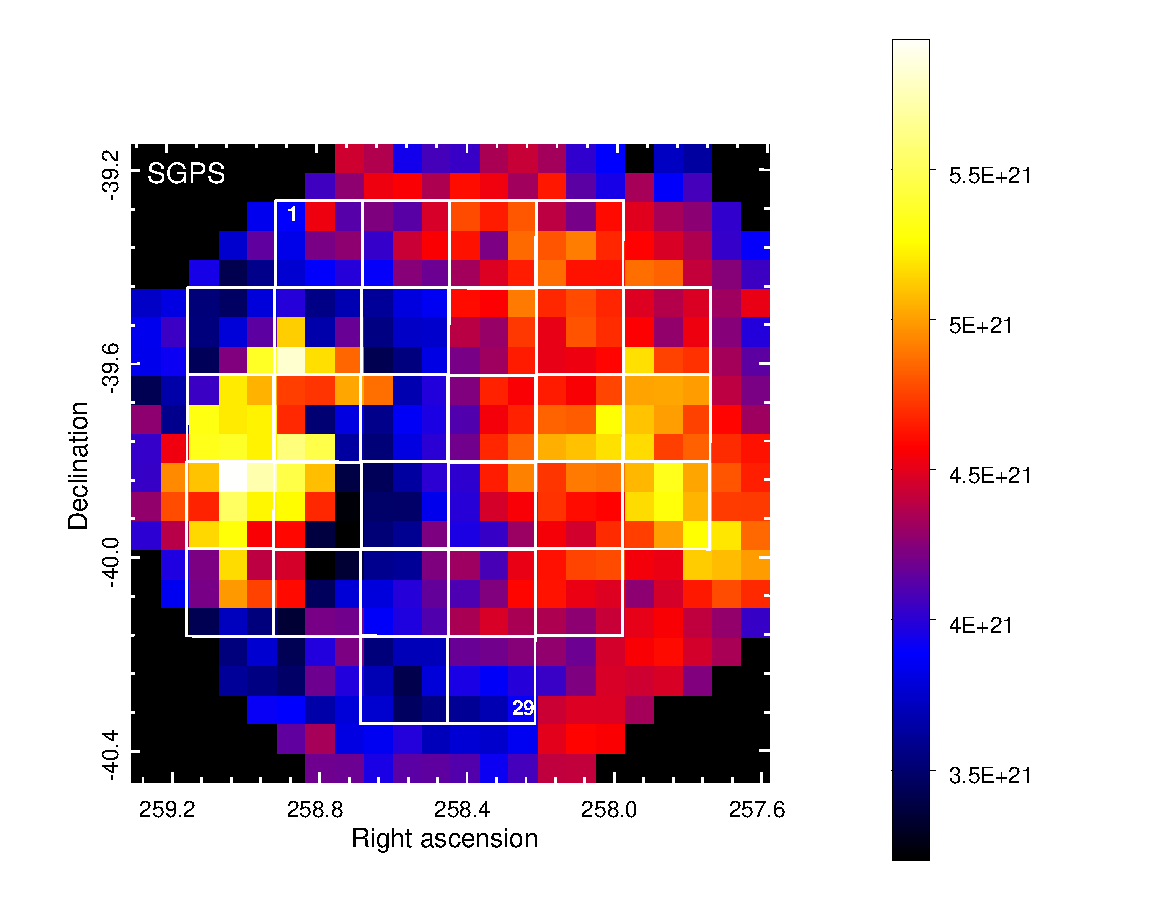
\includegraphics[width=1.05\linewidth, height=0.25\textheight]{HI_9pixels}
	\end{subfigure}
	\begin{subfigure}{0.5\textwidth}
		\centering
		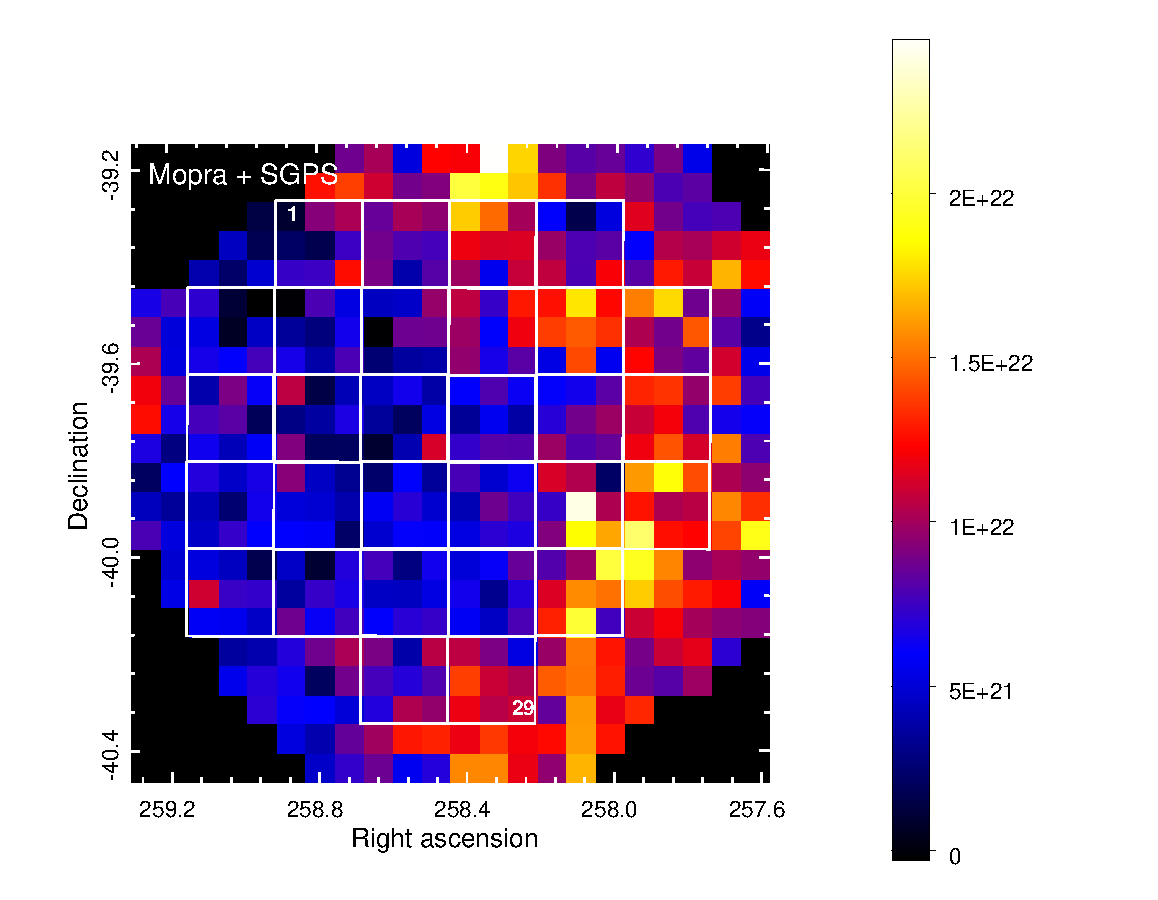
\includegraphics[width=1.05\linewidth, height=0.25\textheight]{mopra_HI_9pixels}
	\end{subfigure}
	\caption{Top left: HESS $\gamma$-ray excess counts for E $>$ 2 TeV, re-binned to fit 9 pixels in each region as described in text. Top right: Mopra $^{12}$CO map, converted to proton column density (cm$^{-2}$) and re-gridded to match the re-binned HESS image. Bottom left: Column density (cm$^{-2}$) of the HI emission derived from the ATCA and Parkes data, re-gridded to match the re-binned HESS image. Bottom right: The HI column density combined with the H$_2$ column density derived from the Mopra data.}
	\label{fig:moprahess9pixels}
\end{figure}


\subsubsection{Error Analysis}
As done in \cite{2012ApJ...746...82F}, the error in the $\gamma$-ray excess counts, $\sigma_{\gamma}$, was calculated simply as the square root of the number of counts. 
\begin{equation}
\label{eq:errgamma}
\sigma_{\gamma} = \sqrt{\mathrm{no. counts}} 
\end{equation}
To obtain the error measurement for the gas column density we calculated the errors in the Mopra, NANTEN and HI data separately and added them accordingly. The error in the Mopra brightness temperature data was derived from the rms noise fluctuations per channel and the number of velocity channels that had been integrated over. The root-mean-square brightness temperature value for each observation was $T_{rms} = 1.5$ K, this is the error in each brightness temperature map for a given velocity channel. Since we integrated over a velocity range of $-20$ km s$^{-1}$ to 0 km s$^{-1}$ and the velocity resolution is $\Delta v = 0.11 $ km s$^{-1}$, we had $N_M = 20 / 0.11 \approx 182 $ total velocity channels (Mopra observations). Using the principles of error propagation for integration (or summing), the error in the velocity-integrated brightness temperature map, $\sigma_I$, is calculated by equation \ref{eq:errint}.
\begin{equation}
\label{eq:errint}
\sigma_I = T_{rms} \times \sqrt{N_M}
\end{equation}
Additionally, the Mopra map was re-gridded to fit the HESS map, so we were required to correct for this error too. The re-gridding processes involved summing over 51 original Mopra pixels to obtain the larger pixel. So, similarly to equation \ref{eq:errint}, the error in the re-gridded Mopra data, $\sigma_R$, followed equation \ref{eq:errregrid}.
\begin{equation}
\label{eq:errregrid}
\sigma_R = \sigma_I \times \dfrac{1}{\sqrt{n}}
\end{equation}
where $n$ is the number of pixels summed over. To convert this into a column density error we simply multiplied by the X factor $X = 2.0 \times 10^{20}$ and the factor of 2 accounting for the double up of protons in the H$_2$ molecules. Hence the error in the proton column density due to the H$_2$ molecules traced by Mopra was found to be
\begin{equation}
\Delta N_{p,\mathrm{M}} = 1.5 \times \sqrt{\dfrac{20}{0.11}} \times \dfrac{1}{\sqrt{51}} \times 2.0 \times 10^{20} \times 2 = 1 \times 10^{21} \ \mathrm{cm}^{-2}
\end{equation}
A similar analysis was used to obtain the error in the Nanten and HI data. Table \ref{tab:erroranal} presents the rms noise fluctuations, velocity resolution and beam size required to calculate the error for all 3 surveys. 
\begin{table}[H] 
	\centering
	\begin{tabular}{c|ccc}
		\toprule
		Telescope & $T_{rms}$ (K) & $\Delta v$ (km s$^{-1}$) & Beam Size \\
		\hline 
		Mopra & 1.5 & 0.11 & 35$^{\prime \prime}$ \\
		Nanten & 0.3 & 0.65 & 2.6$^\prime$\\
		SGPS & 1.6 & 0.82 & 2.2$^\prime$\\
		\bottomrule
	\end{tabular} 
	\caption{The rms noise fluctuations and velocity resolution for the Mopra, NANTEN and SGPS surveys.}
	\label{tab:erroranal}
\end{table}
We calculated the error in the proton column density due to the H$_2$ molecules traced by Nanten to be
\begin{equation}
\Delta N_{p,\mathrm{N}} = 0.3 \times \sqrt{\dfrac{20}{0.65}} \times \dfrac{1}{\sqrt{2}} \times 2.0 \times 10^{20} \times 2 = 0.5 \times 10^{21} \ \mathrm{cm}^{-2}
\end{equation}
where we have included the extra factor of 2 to account for the molecular to atomic conversion and used the same velocity range as the Mopra data. Lastly, for the HI data we use the same velocity range as Mopra and included the factor of $1.823 \times 10^{18}$ from equation \ref{eq:HIcoldens}. We calculated the error in the proton column density due to the observed atomic hydrogen to be,
\begin{equation}
\Delta N_{p,\mathrm{HI}} =  1.6 \times \sqrt{\dfrac{20}{0.82}} \times \dfrac{1}{\sqrt{3}} \times  1.823 \times 10^{18} = 0.01 \times 10^{22} \ \mathrm{cm}^{-2} \ .
\end{equation} 


\subsubsection{Data Analysis - Bootstrapping}
To quantify the correlation between the gas density and the $\gamma$-ray flux we utilised the Pearson correlation coefficient, $\rho$, (equation \ref{eq:pearsons}). The Pearson correlation coefficient is a measure of the linear correlation between two variables and takes on a value between -1 and +1. A value of +1 indicates a perfect, positive-linear relationship, a value of 0 indicates no linear relationship and a value of -1 indicates a perfect, negative-linear relationship. 
\begin{equation}\label{eq:pearsons}
\rho = \dfrac{\mathrm{cov}(X,Y)}{\sigma_X \sigma_Y}
\end{equation}
where cov($X,Y)$ is the covariance (equation \ref{eq:covariance}) of both data sets and $\sigma_X$, $\sigma_Y$ are the standard deviations (equation \ref{eq:stddev}) of the X and Y data (proton column density and $\gamma$-ray excess counts), respectively.
\begin{equation}\label{eq:covariance}
\mathrm{cov}(X,Y) = \dfrac{1}{n} \sum_{i=1}^n (x_i - \bar{x})(y_i - \bar{y})
\end{equation}
where n is the number of measurements in the data set, $x_i$ and $y_i$ are the individual measurements and $\bar{x}$ and $\bar{y}$ are the means of each data set.
\begin{equation}\label{eq:stddev}
\sigma_X = \sqrt{\dfrac{\sum_{i=1}^n (x_i - \bar{x})^2}{n -1}}
\end{equation}

If we expect the hadronic scenario to be dominant, then the relationship between the $\gamma$-ray flux and the gas density should be positive amd linear, recall equation \ref{eq:5},
\begin{equation} 
\Phi_{\gamma} = 4 \pi n_H \int \dfrac{d\sigma}{dE_\gamma} \dfrac{dN_p}{dE_p} dE_p \ .
\end{equation}
Whereas, if the hadronic scenario is not dominant, this positive-linear relationship shouldn't be observed. 

The 9 pixels in each region were used as the data sets and we analysed the gas density maps from Mopra and NANTEN separately. 

Since $\rho$ doesn't incorporate the individual error from each data point, we employ a bootstrapping technique. 
We take each data point from the set and randomly re-distribute it in both x and y directions assuming it follows a normal distribution. 
The actual x-y values are taken as the means, while the errors in each direction are taken as the standard deviations. 
An example of this randomization is shown in figure \ref{fig:bootstrap example} (left). 
This new, randomised data set will produce a new $\rho$ value, reiterating the process multiple times will give us a distribution of values. 
Figure \ref{fig:bootstrap example} (right) shows the distribution obtained for region 1 after 100 000 iterations were performed. 

\begin{figure}[H]
	\begin{subfigure}{0.47\textwidth}
		\centering
		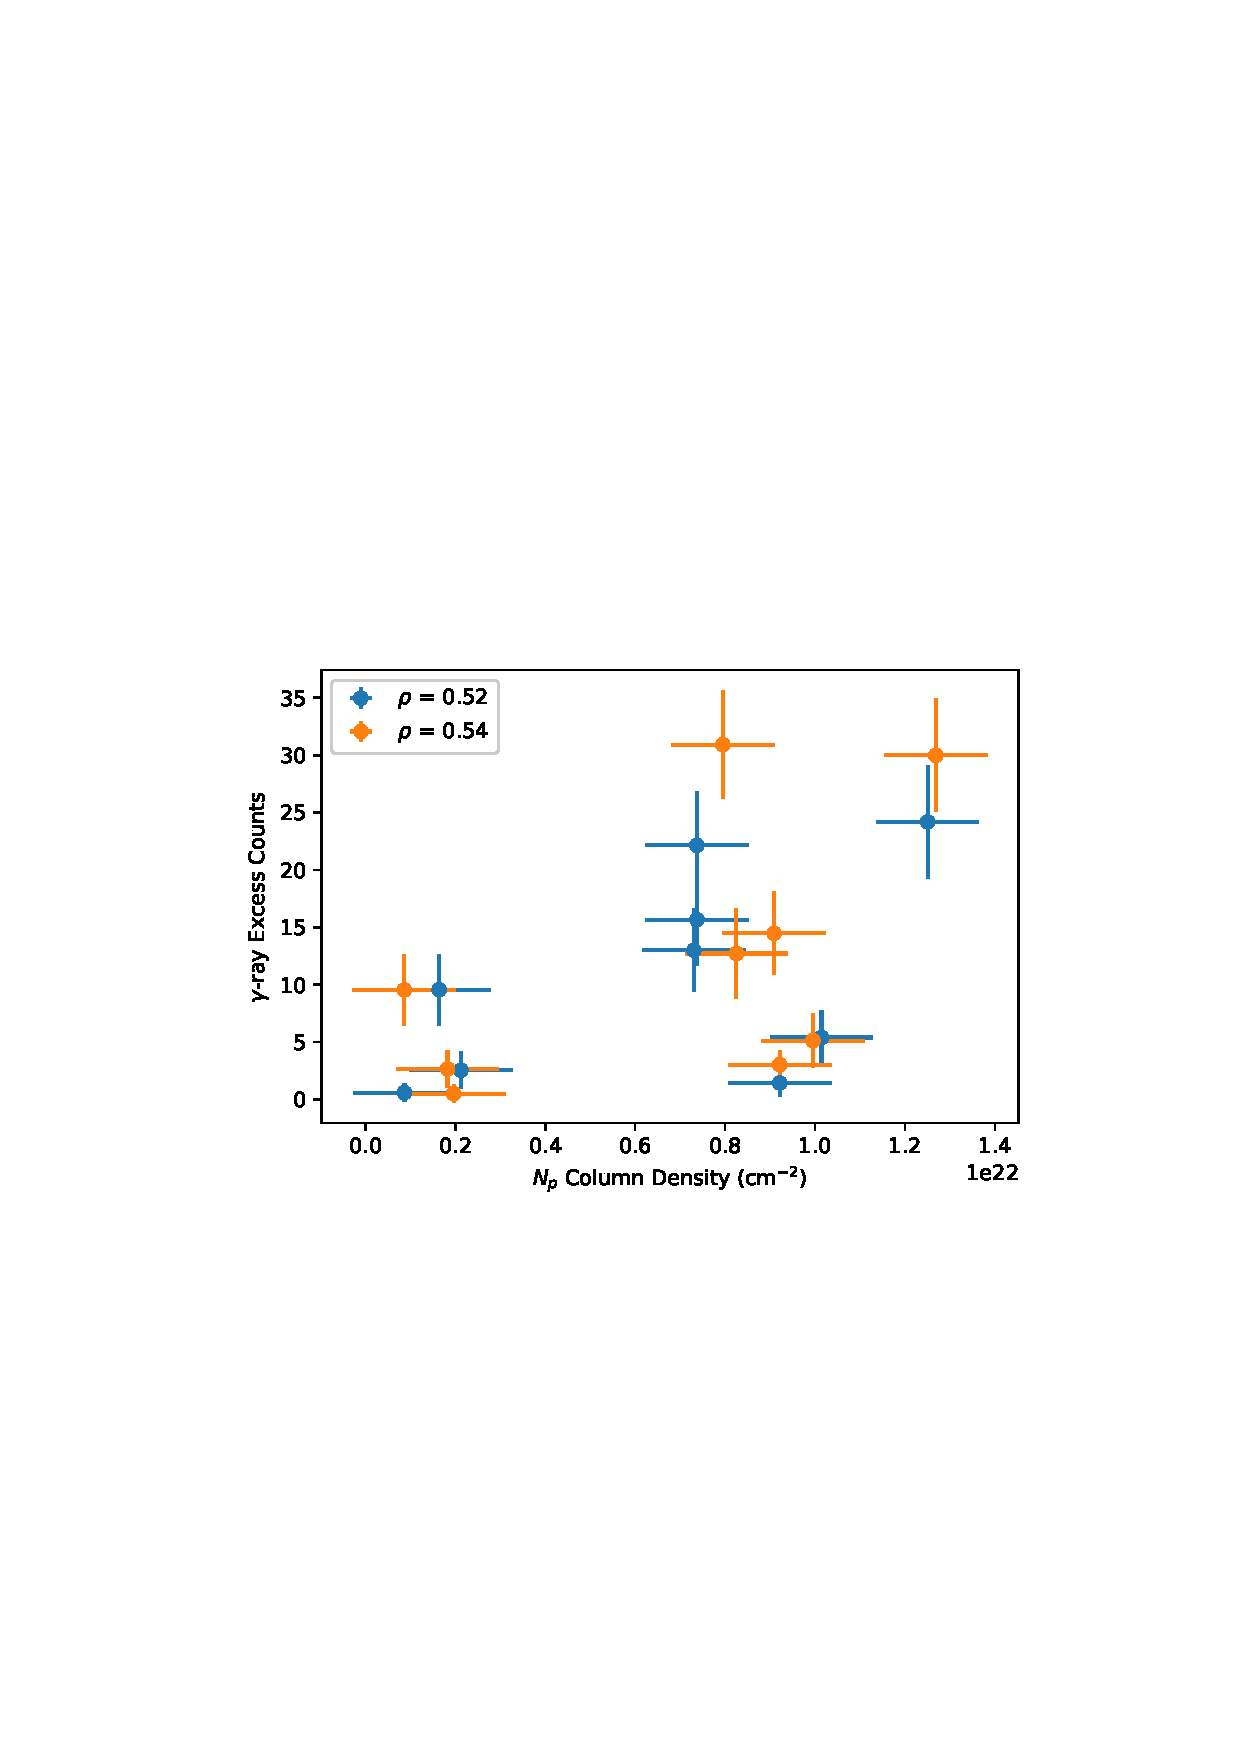
\includegraphics[width=0.95\linewidth, height=0.22\textheight]{bootstrap_example}
	\end{subfigure}
	\begin{subfigure}{0.53\textwidth}
		\centering
		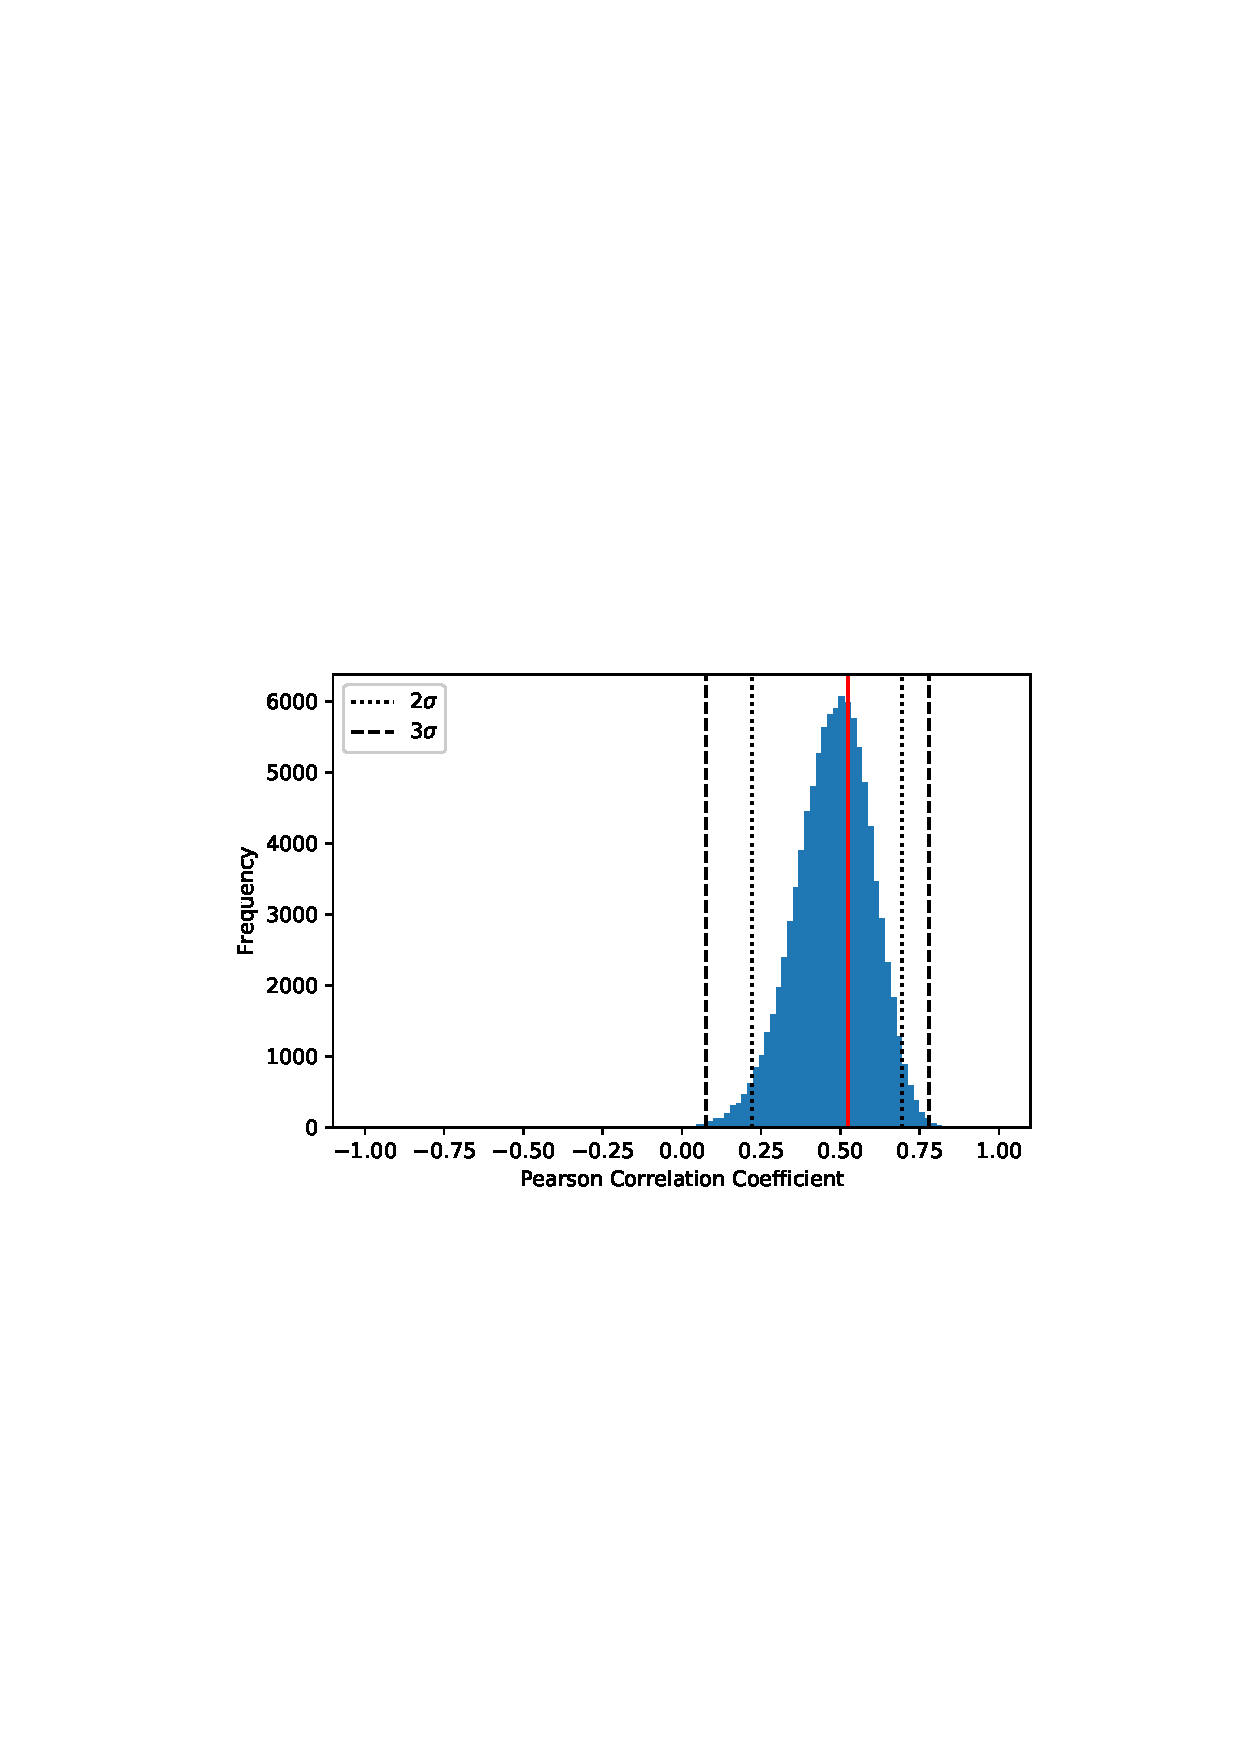
\includegraphics[width=0.95\linewidth, height=0.22\textheight]{gammopHI_reg1}
	\end{subfigure}
	\caption{An example of bootstrapping the $\gamma$-ray and $N_p$ column density data set for region 1. Left: The original data points (blue) plotted and compared against a single set of randomised data points (orange), as described in text. The same error bars are used on both data sets. Right: The distribution of $\rho$ value's calculated from a total of 100 000 randomisations. The red line signifies the $\rho$ value of the original data set, while the dotted line and the dashed line represent the 2$\sigma$ and 3$\sigma$ values respectively.}
	\label{fig:bootstrap example}
\end{figure}

We take our original $\rho$ to be our final value but we quote the significance of some optimistic value $\rho_\mathrm{o}$ (e.g. the 3 $\sigma$ value). The significance is determined by calculating the probability that a randomly distributed data set will produce the same optimistic $\rho$ value.


\subsubsection{Results}
Table \ref{tab:gasgammacor} presents the Pearson correlation coefficient, $\rho$, for the gas density and $\gamma$-ray flux in each region and for both Mopra and NANTEN data sets. Additionally, the optimistic (3 $\sigma$) value, $\rho_\mathrm{o}$, is specified along with its significance.
\begin{table}[H] 
	\centering
	\begin{tabular}{ccccccccc}
		\toprule 
		&&
		\multicolumn{3}{c}{Mopra} 
		&&
		\multicolumn{3}{c}{Nanten} \\
		\cline{2-5} \cline{7-9} 
		Reg. && $\rho$ & $\rho_\mathrm{o}$ & Significance && $\rho$ & $\rho_\mathrm{o}$ & Significance \\
		\hline 
		1 && 0.52 & 0.78 & 2 $\sigma$ && -0.06 & 0.877 & no \\
		2 && -0.29 & -0.86 & 2 $\sigma$ && -0.67 & 0.046 & yes \\
		3 && -0.71 & -0.91 & 3 $\sigma$ && -0.74 & 0.023 & yes \\
		4 && 0.80 & 0.95 & 4 $\sigma$ && 0.24 & 0.531 & no \\
		5 && 0.09 & 0.63 & 1 $\sigma$ && 0.88 & 0.002 & yes \\
		6 && -0.00 & -0.82 & 2 $\sigma$ && 0.01 & 0.987 & no \\ 
		7 && 0.01 & 0.80 & 2 $\sigma$ && -0.07 & 0.856 & no \\
		8 && 0.02 & 0.65 & 1 $\sigma$ && 0.10 & 0.806 & no \\
		9 && 0.38 & 0.82 & 2 $\sigma$ && 0.56 & 0.115 & no \\
		10 && 0.11 & 0.62 & 1 $\sigma$ && 0.06 & 0.883 & no \\
		11 && -0.04 & -0.74 & 2 $\sigma$ && 0.57 & 0.110 & no \\
		12 && 0.54 & 0.90 & 3 $\sigma$ && 0.77 & 0.015 & yes \\
		13 && -0.02 & -0.82 & 2 $\sigma$ && -0.26 & 0.493 & no \\
		14 && -0.74 & -0.93 & 3 $\sigma$ && 0.21 & 0.585 & no \\
		15 && 0.34 & 0.87 & 3 $\sigma$ && 0.75 & 0.019 & yes \\
		16 && 0.80 & 0.93 & 3 $\sigma$ && 0.15 & 0.692 & no \\ 
		17 && -0.11 & -0.80 & 2 $\sigma$ && 0.27 & 0.480 & no \\
		18 && 0.56 & 0.90 & 3 $\sigma$ && 0.63 & 0.066 & no \\
		19 && 0.13 & 0.83 & 2 $\sigma$ && -0.35 & 0.352 & no \\
		20 && 0.02 & 0.79 & 2 $\sigma$ && 0.53 & 0.143 & no \\
		21 && 0.49 & 0.88 & 3 $\sigma$ && 0.73 & 0.025 & yes \\
		22 && 0.44 & 0.87 & 3 $\sigma$ && 0.40 & 0.287 & no \\
		23 && -0.62 & -0.87 & 3 $\sigma$ && -0.21 & 0.579 & no \\
		24 && -0.25 & -0.83 & 2 $\sigma$ && -0.08 & 0.837 & no \\
		25 && 0.12 & 0.77 & 2 $\sigma$ && -0.26 & 0.492 & no \\
		26 && -0.02 & -0.82 & 2 $\sigma$ && 0.42 & 0.261 & no \\ 
		27 && 0.24 & 0.80 & 2 $\sigma$ && 0.46 & 0.217 & no \\
		28 && 0.04 & 0.71 & 2 $\sigma$ && -0.22 & 0.570 & no \\
		29 && -0.40 & -0.85 & 2 $\sigma$ && -0.42 & 0.258 & no \\
		\hline 
	\end{tabular} 
	\caption{The calculated Pearson correlation coefficient, the optimistic Pearson coefficient and the associated significance, for the gas density and the HESS $\gamma$-ray flux ($> 2$ TeV) data for each region and for both Mopra and NANTEN data sets.}
	\label{tab:gasgammacor}
\end{table}
A scatter plot for each region was also produced and fitted with a line of best fit, illustrating the correlation between the gas density and the HESS $\gamma$-rays. Figure \ref{fig:regionalgasgammacormop} illustrates some such plots with the gas density calculated with the Mopra data. Only plots for regions which contained significant correlations are illustrated.


\begin{figure}[H]
	\begin{subfigure}{0.5\textwidth}
		\centering
		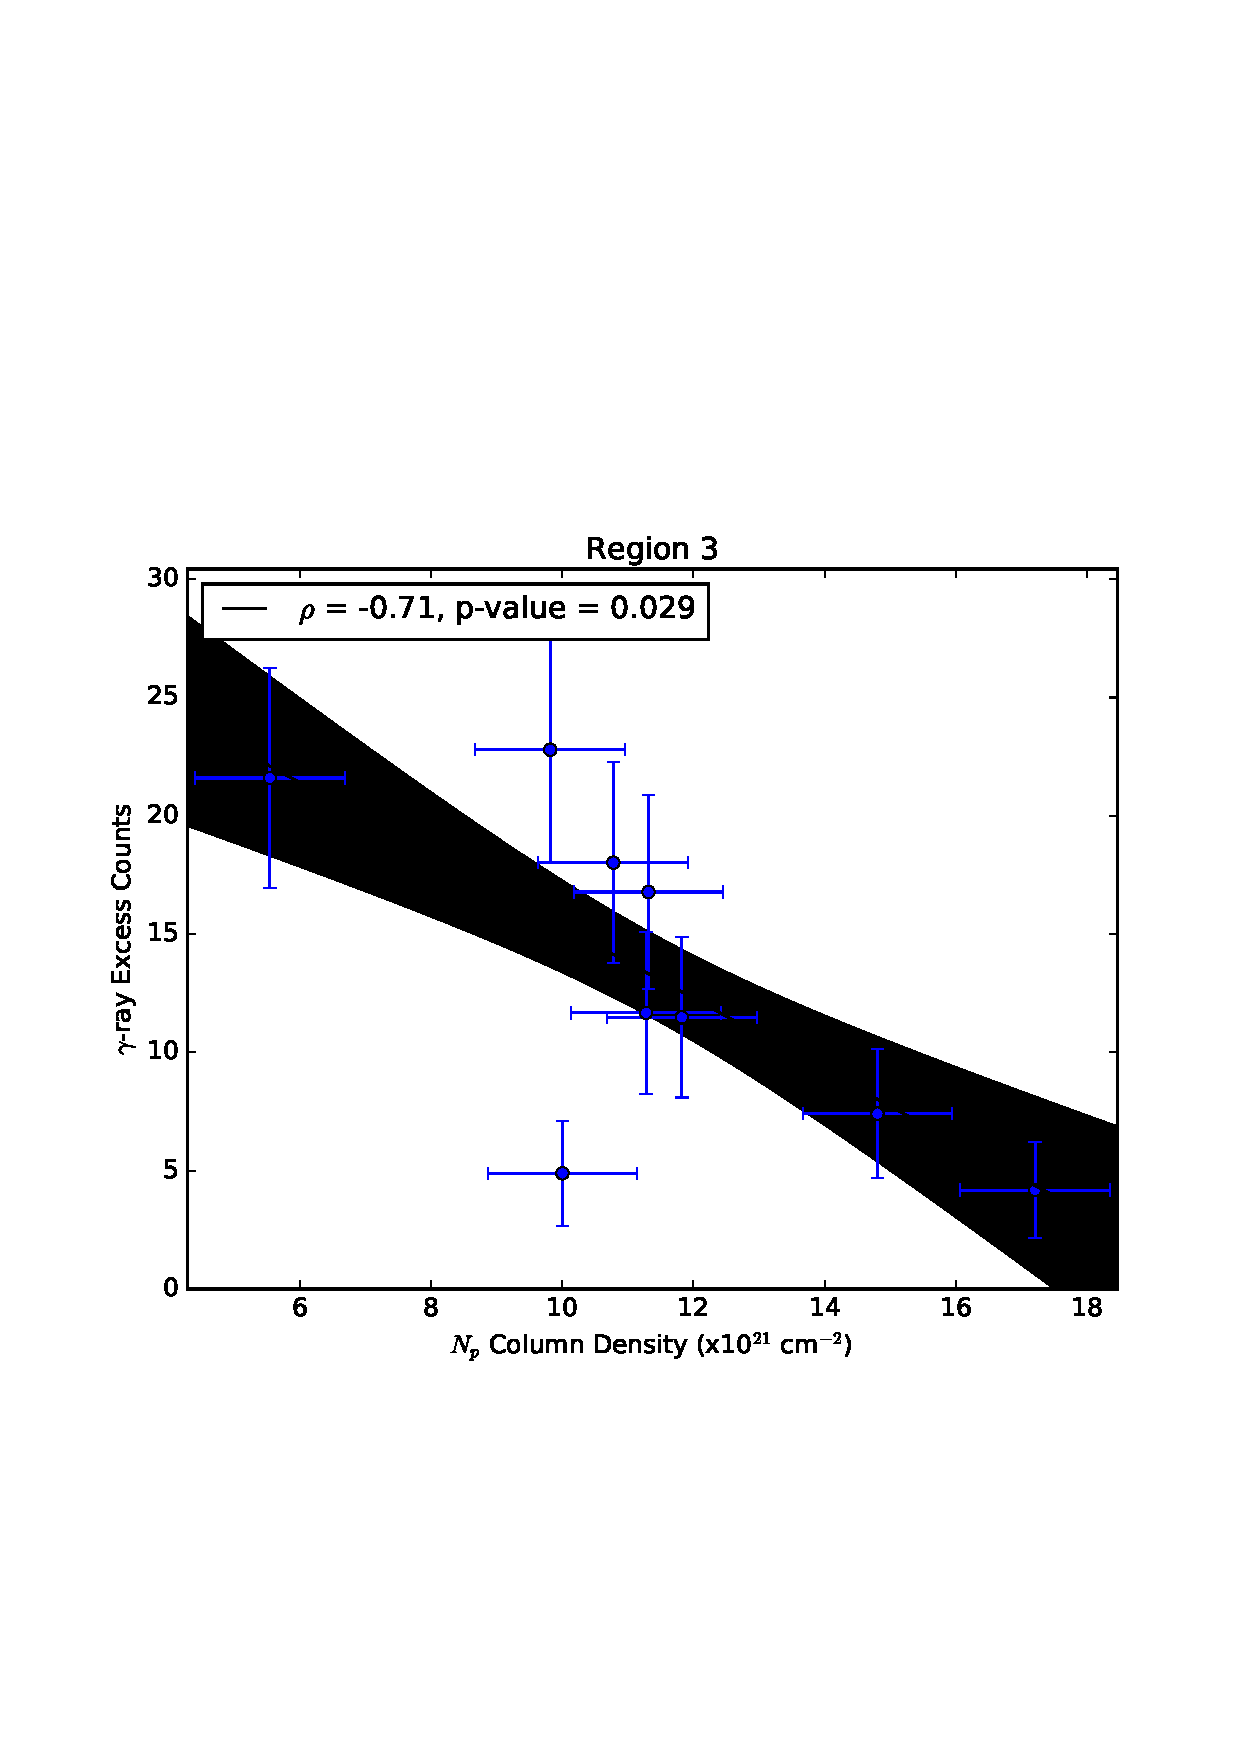
\includegraphics[width=0.95\linewidth, height=0.27\textheight]{gamma_mHI_reg3}
		\label{fig:gmHIreg3}
	\end{subfigure}
	\begin{subfigure}{0.5\textwidth}
		\centering
		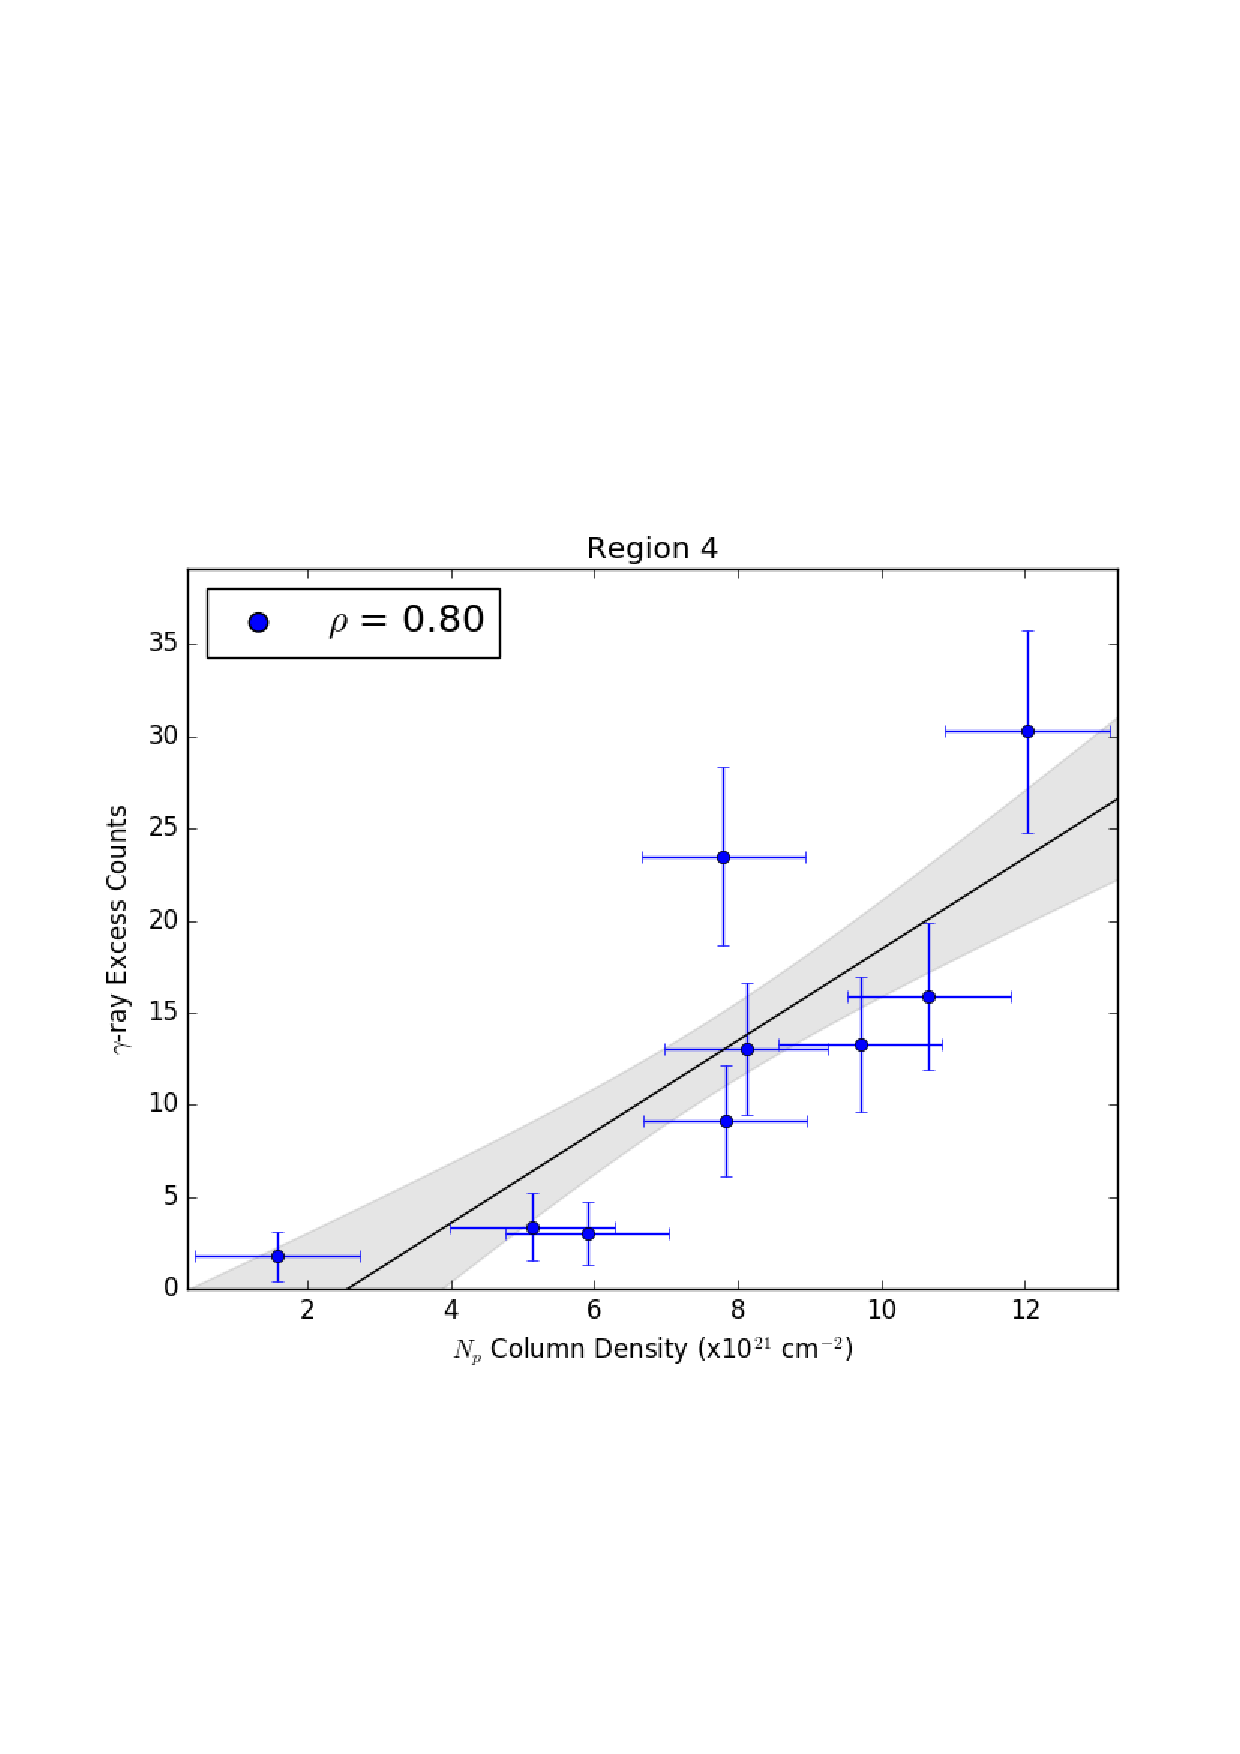
\includegraphics[width=0.9\linewidth, height=0.27\textheight]{gamma_mHI_reg4}
		\label{fig:gmHIreg4}
	\end{subfigure}
	\begin{subfigure}{0.5\textwidth}
		\centering
		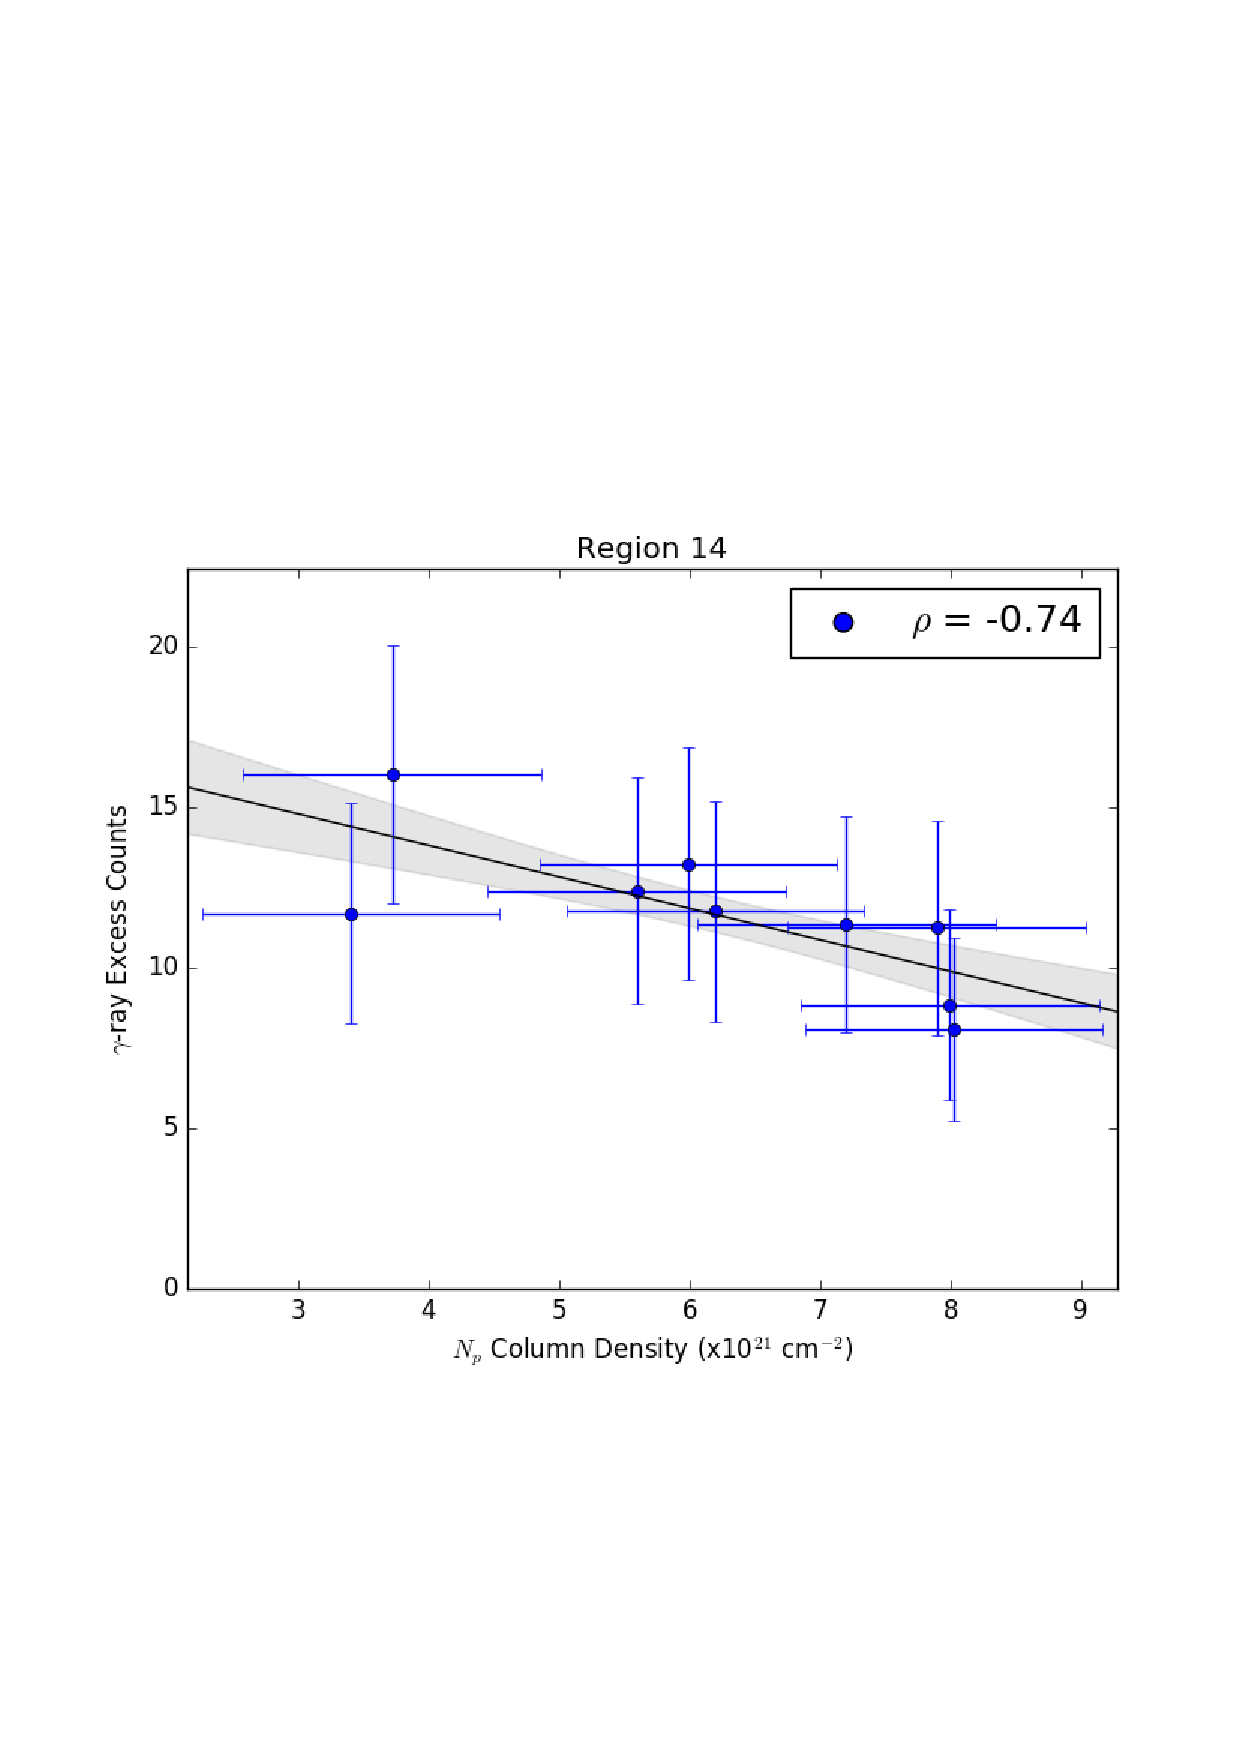
\includegraphics[width=0.9\linewidth, height=0.27\textheight]{gamma_mHI_reg14}
		\label{fig:gmHIreg14}
	\end{subfigure}
	\begin{subfigure}{0.5\textwidth}
		\centering
		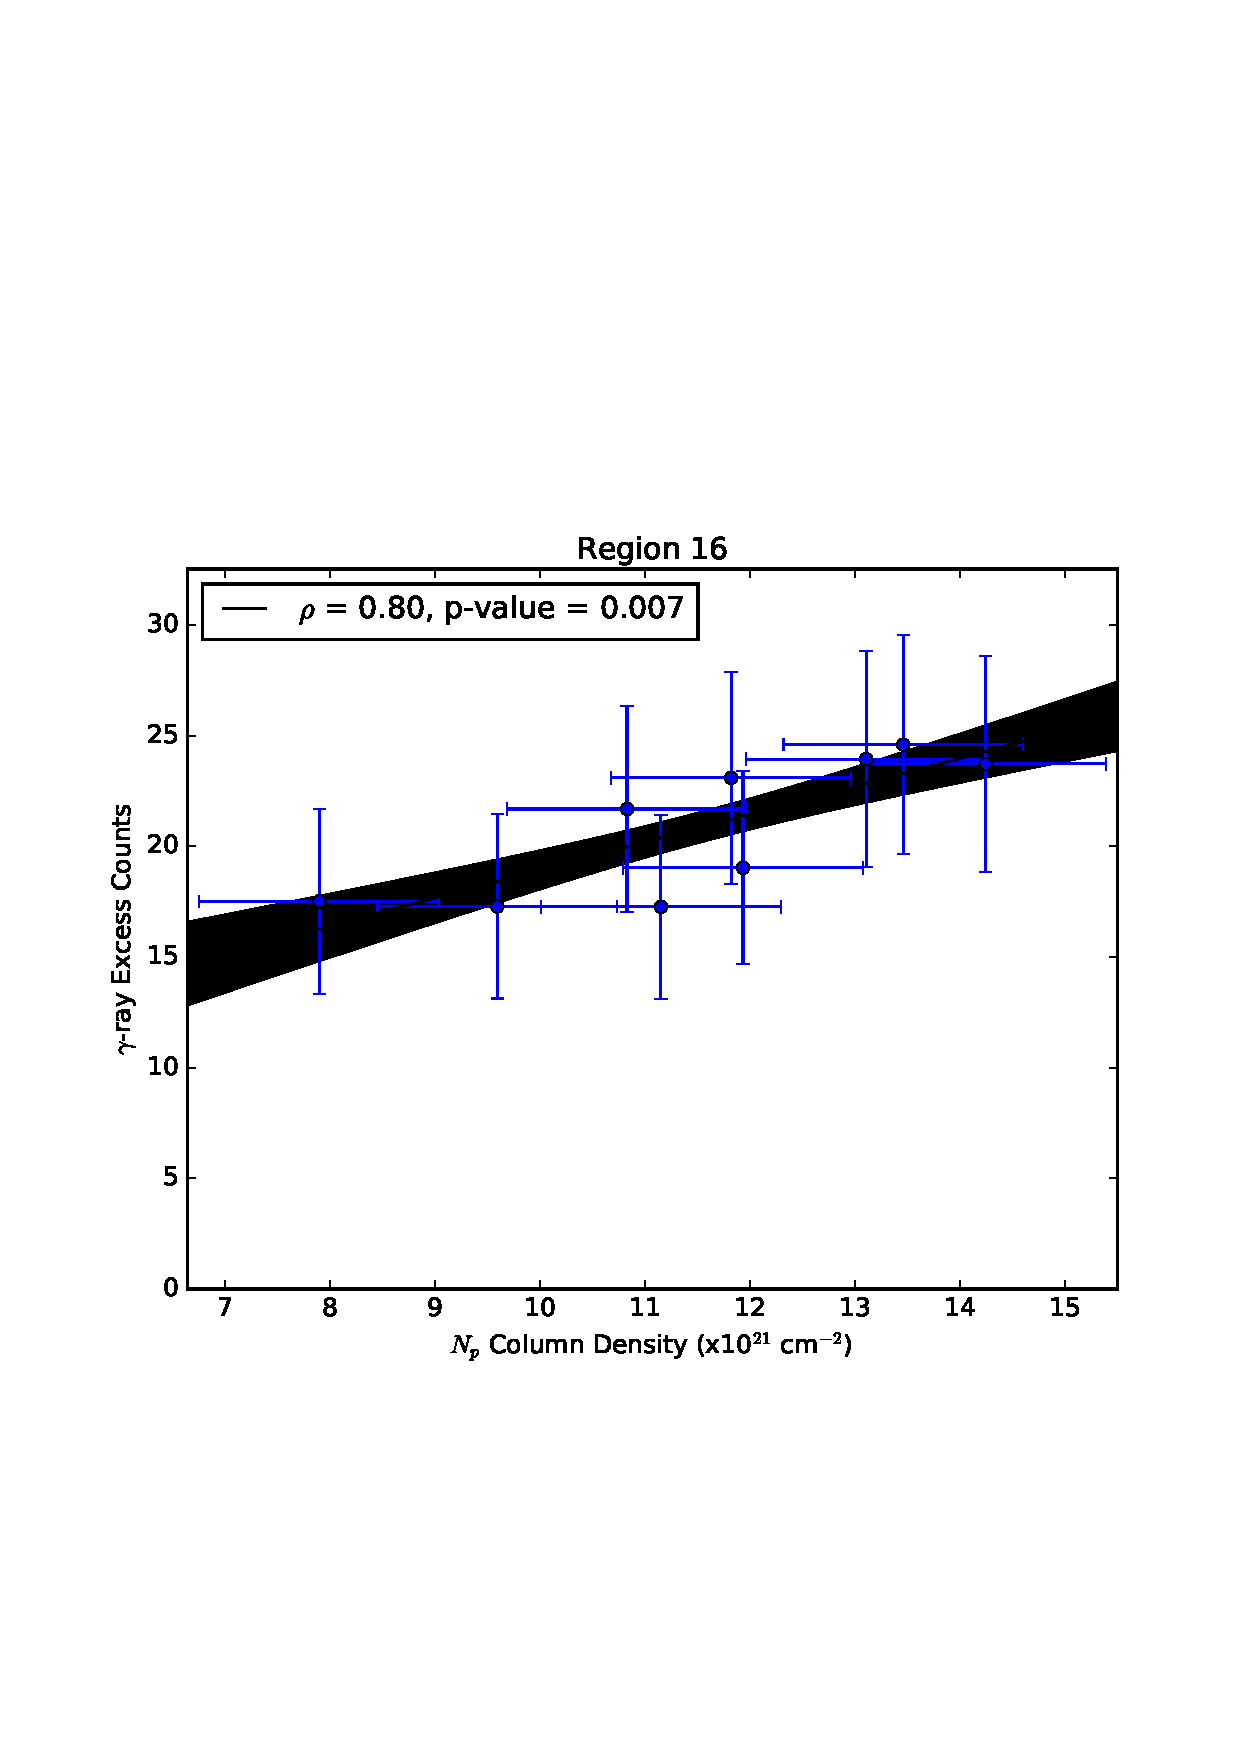
\includegraphics[width=0.9\linewidth, height=0.27\textheight]{gamma_mHI_reg16}
		\label{fig:gmHIreg16}
	\end{subfigure}
	\caption{Correlation plots between the ISM gas density and $\gamma$-ray flux using the Mopra $^{12}$CO data for the molecular component of the gas density. The line of best fit for each data set is shown in black, while the grey area illustrates the confidence bands. Regions that display significant correlations are shown.}
	\label{fig:regionalgasgammacormop}
\end{figure}

As can be seen in table \ref{tab:gasgammacor}, few regions have statistically significant p-values with either the Mopra or NANTEN data sets (regions 2, 3, 4, 5, 12, 14, 15, 16 and 21). More importantly, only region 3 had a consistent significant p-value for both data sets. A positive correlation was found between the ISM gas density and $\gamma$-ray flux for regions 4, 5, 12, 15, 16 and 21. Although these significant correlations were only seen for one data set, the \textit{other} data set still always produced a positive correlation regardless of the significance. Also, significant negative correlations were found for regions 2, 3 and 14. 

Using the results from the Mopra datset, we then categorised each region according to their correlation and significance and portrayed the results as a colour-scale plot (figure \ref{fig:colourcoderegions}: Left). Regions with a significant positive correlation were coloured magenta, regions with an insignificant positive correlation $> 0.25$ were coloured brown, regions with a significant negative correlation were coloured white, regions with an insignificant negative correlation $ < -0.25$ were coloured teal green and lastly, regions with correlations between $-0.25$ and $0.25$ were coloured lime green. There appears to be signs of positive correlation along the eastern rim of the SNR. These regions are also observed to produce a large flux of TeV $\gamma$-rays. We also note that regions at the centre of the SNR corresponding to the shell cavity have either no correlation or a negative correlation. There doesn't appear to be any significant correlation on the western side of the SNR, the gas doesn't appear to be dense here either, yet $\gamma$-ray emission is still observed.

\subsubsection{Discussion}
We propose a scenario to explain our observations and results assuming the dominant process producing the $\gamma$-rays is hadronic. 1600 years ago a supernova occurred at approximately the centre of our source. As the stellar wind of the SNR projects outwards, the shock along with accelerated protons may begin interacting with any ISM gas may or may not be present. As the shock propagates further outwards it also pushes the gas further outwards, causing it to collect on the outer shell of the shock front. As the gas propagates with the shock front, accelerated protons would continue to interact with the gas (PP interactions) and continually produce $\gamma$-rays. ISM gas would collect and be most dense on the outer shell formed by the shock front. Gas beyond this outer shell would be untouched by the CR protons unless they have already escaped from the SNR. As the SNR is still young we only expect high energy protons to have escaped ($>150$ TeV) \citep{2010PASJ...62.1127C}. For this reason we assume that the shock front is currently spatially correlated with a shell-like region just within the outer rim of the observed $\gamma$-rays.

\begin{figure}[H]
	\begin{subfigure}{0.5\textwidth}
		\centering
		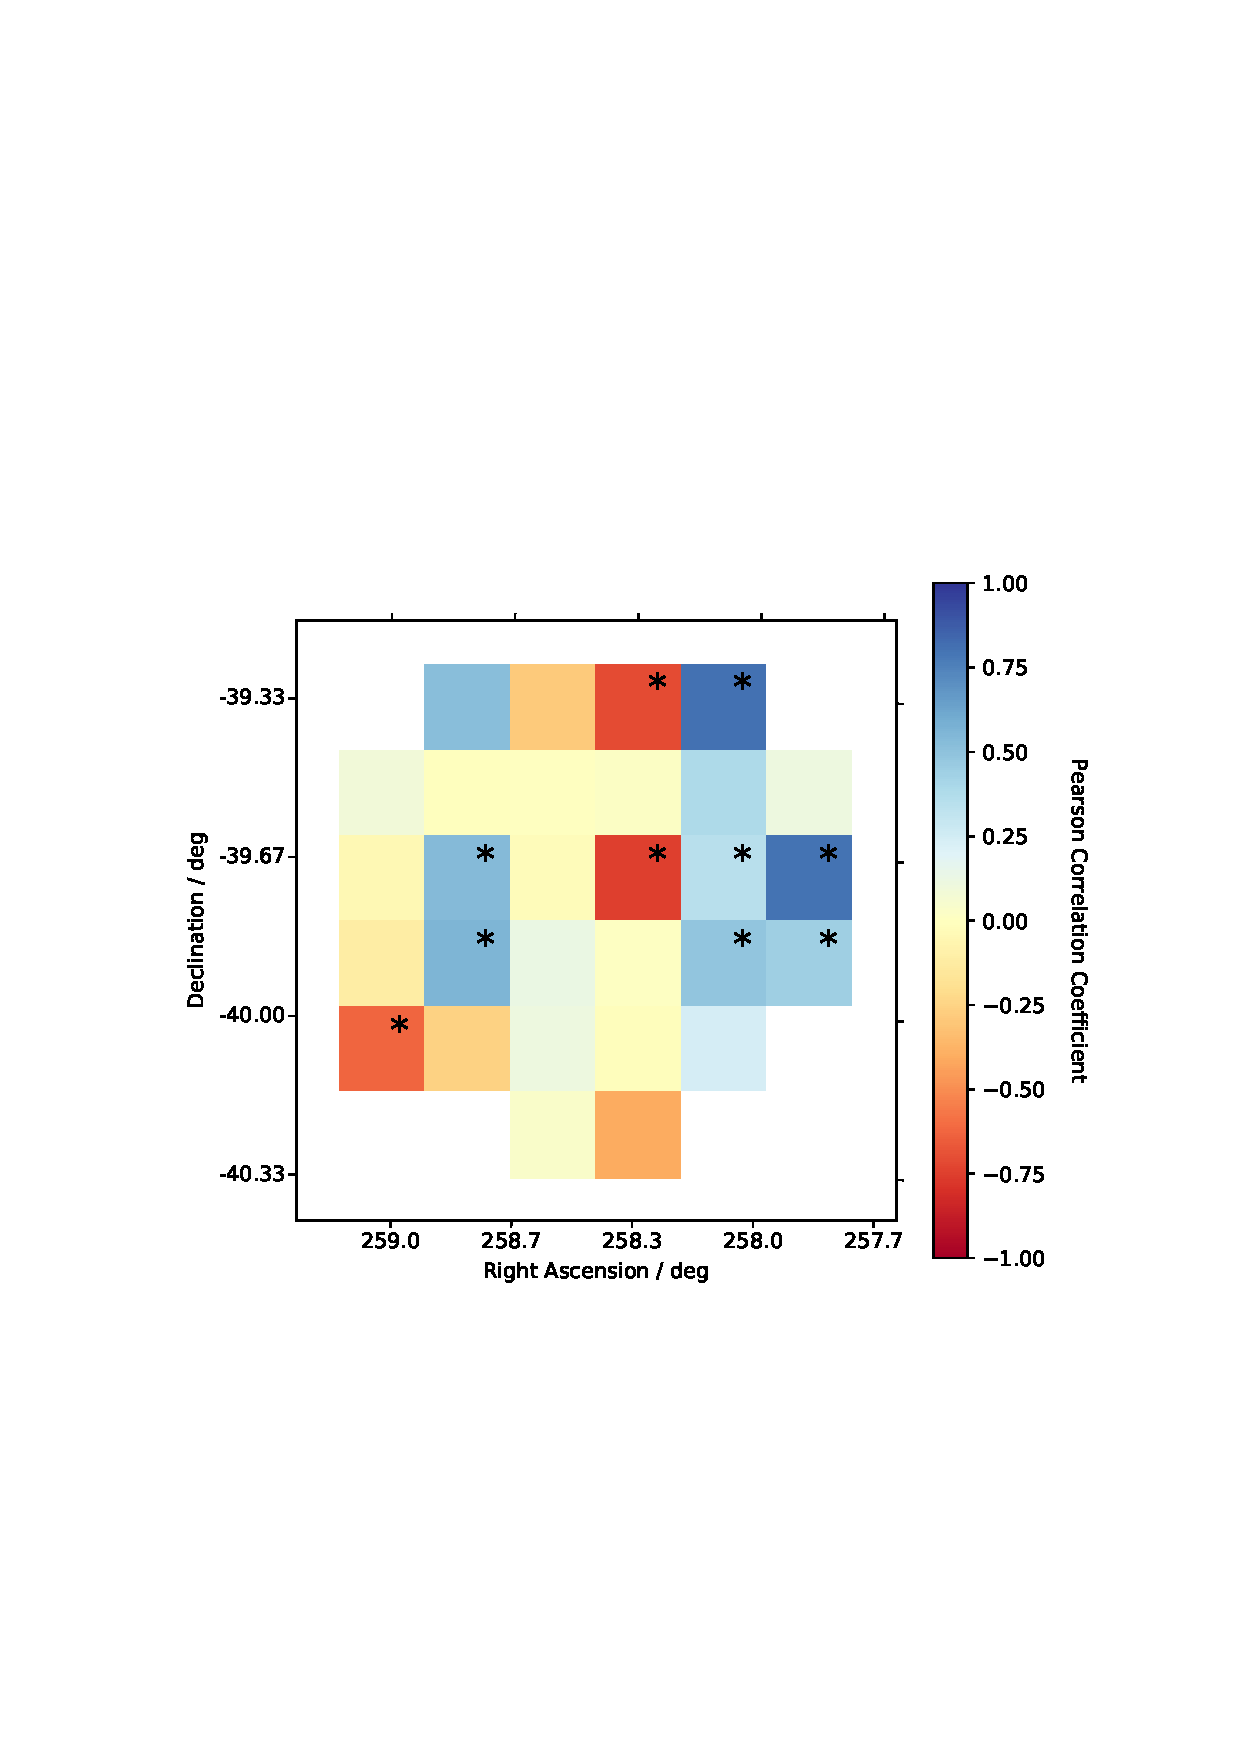
\includegraphics[width=1.00\linewidth, height=0.25\textheight]{pearsonmap_gam_mopHI}
		\label{fig:corsigmap}
	\end{subfigure}
	\begin{subfigure}{0.5\textwidth}
		\centering
		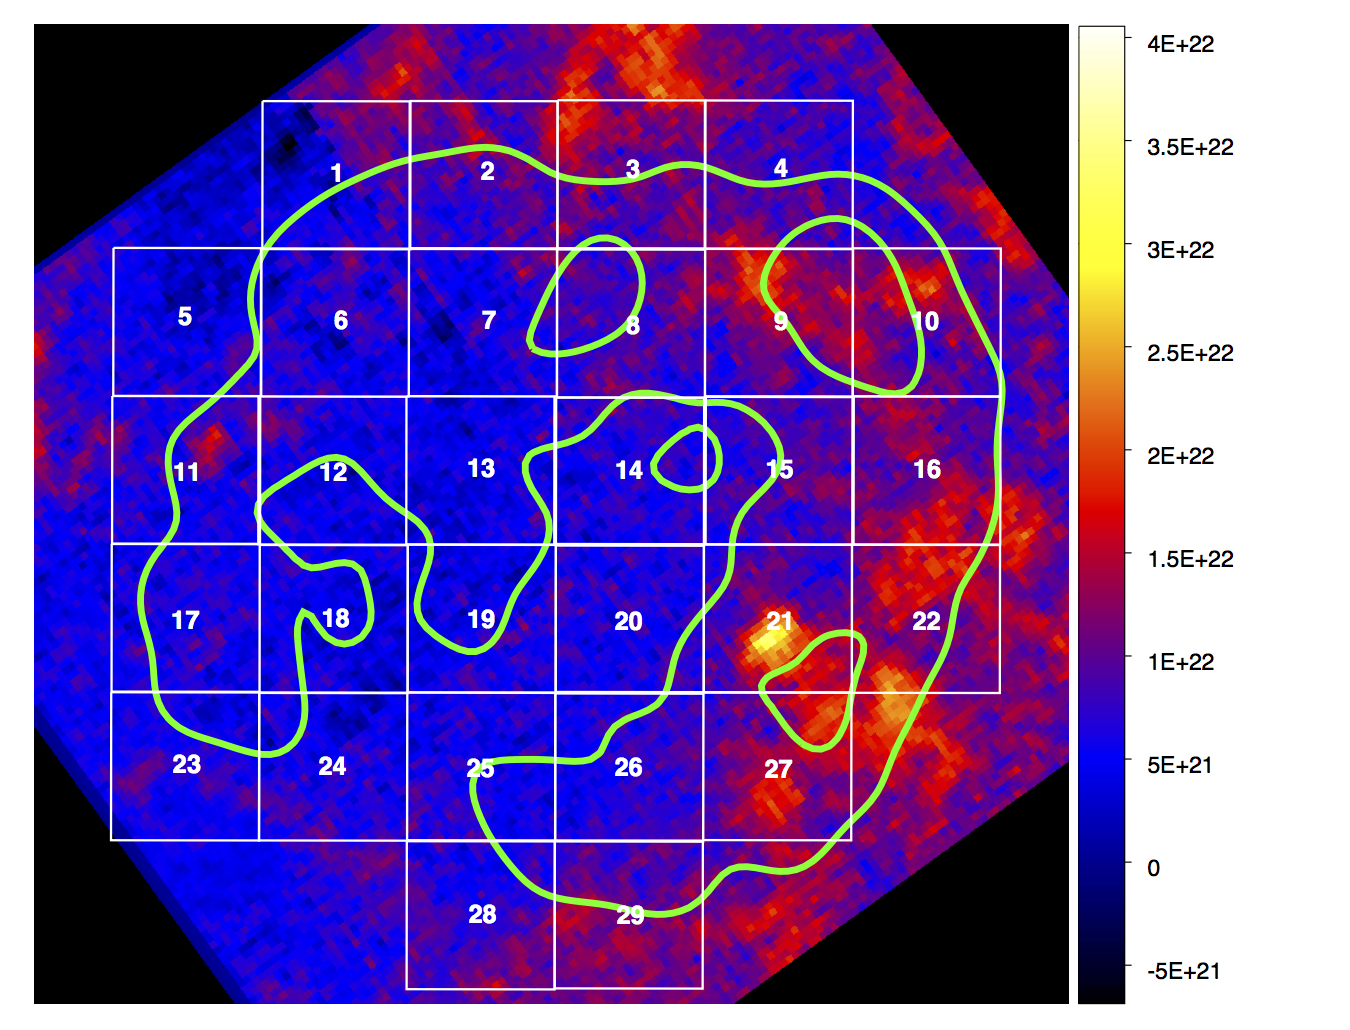
\includegraphics[width=1.00\linewidth, height=0.25\textheight]{mopra_HI_hesscont}
		\label{fig:wpratiomap}
	\end{subfigure}
	\caption{Left: A colour map portraying each region according to their Pearson's correlation	coefficient. Regions containing a dot are those with significance $>2 \sigma$ Right: Total ISM gas column density calculated with the SGPS and Mopra datsets, overlaid with the 29 regions in white and the HESS ($>2$ TeV) $\gamma$-ray contours in green.}
	\label{fig:colourcoderegions}
\end{figure}

Highly dense gas is seen all across the eastern side of the SNR source (figure \ref{fig:colourcoderegions}: right). The gas here has likely been collected by the shock front. Note that this map is in units of column density, it is the sum of the gas along that line of sight, so the gas we see is likely not all concentrated into one dense spot. Positive correlations were seen in regions along the east (regions 9, 15, 16, 21 and 22). According to our scenario much of the gas has been expelled from regions 9, 15 and 21 already. Hence the $\gamma$-rays are most likely hadronic in origin, yet the gas is no longer as spatially correlated as it would have been, explaining why we don't see a \textit{significant} correlation. 

Region 16 is situated over the current position of the shock front, hence the gas is still spatially correlated with the $\gamma$-rays it produced in this region. Region 4 is similar again, there appears to be a build up of gas within the shell and less gas beyond the shell, providing a perfect example for our proposed scenario. The significant positive correlation for these 2 regions coincides well with our argument. Region 22 appears to have characteristics consistent with our scenario, however the positive correlation is not significant. Region 10 is seen to exhibit no correlation between the gas density and the $\gamma$-ray flux. This could be due to the region of peak $\gamma$-ray emission (illustrated by the green contours) no longer being spatially correlating with the dense gas as it has been pushed out by the shock front.

On the north side we still see dense gas except it is predominantly external from the $\gamma$-ray shell and likely beyond the reach of the shock front and CR protons. Region 3 stands out because it displays a very high density of untouched gas beyond the $\gamma$-ray shell, this explains the significant negative correlation we see. Region 2 is much the same however the untouched gas is not as dense, hence the correlation isn't as significant. Region 4 is not included in this argument because the gas does not appear as dense beyond the shell, but rather more dense within the shell, pertaining to the argument made in the previous paragraph. Region 1 is appears to contain a combination of untouched dense gas and a void of gas beyond the $\gamma$-ray shell. This void of gas contributes to the positive correlation we see in this region and is due to shock front not yet reaching this part of the region. 

At the centre of the SNR in regions 14 and 20 we don't see an intense flux of $\gamma$-rays so we suggest that when the SNR was younger and much smaller there wasn't much gas close enough to allow PP interactions to occur. Alternatively, the CR protons did not have enough time to undergo PP interactions with the gas as the shock would have been traveling with greater velocity and propagated beyond this region. However, region 14 does display a small peak of $\gamma$-ray emission, which if produced by PP interactions the gas has long been swept up and pushed outwards. This explains the negative correlation between the gas and $\gamma$-rays seen in region 14.

Regions 13 and 19 on the western side of the centre of the SNR appear to lack dense gas, yet there is $\gamma$-ray emission observed. There does not appear to be much dense gas further west either, so it is likely that PP interactions are not the main contributor to the $\gamma$-ray flux seen in these regions. The same can be said for the entire western side from regions 5 and 6 down to 23 and 24. Regions 12 and 18 show a positive correlation suggesting that the gas may be responsible for a slight contribution of the $\gamma$-ray flux. By the time the shock had propagated to these two regions, CR protons may have had enough time to undergo PP interactions. We also see evidence of some gas remaining at these locations, explaining the positive correlation. Overall, the TeV emission in these western regions is likely dominated by IC scattering. 

Regions 28 and 29 covering the southernmost point of the SNR appear to have dense gas situated beyond the shock front much like that of regions 2 and 3. The protons have not yet reached this gas but have interacted with the gas within the shell producing the $\gamma$-ray flux seen on the northern parts of these regions. However the gas is beginning to be pushed outwards by the shock front, hence it is not spatially correlated with the $\gamma$-rays. 

We have argued that regions located on the eastern side of RX J1713.7-3946 have a $\gamma$-ray flux which is dominated by hadronic production due to the high density of the gas and in some cases the positive correlation between the gas density and $\gamma$-rays. There is still likely a leptonic component due to the observed X-rays in this region (figure \ref{fig:suzakumap}). Regions along the northern and southern rim were also argued to have a major hadronic component related to their $\gamma$-ray emission. We have also argued that the $\gamma$-rays on the western side are produced by IC scattering due to the lack of gas and lack of spatial correlation between the gas and $\gamma$-rays. 

\begin{figure}[H]
	\centering
	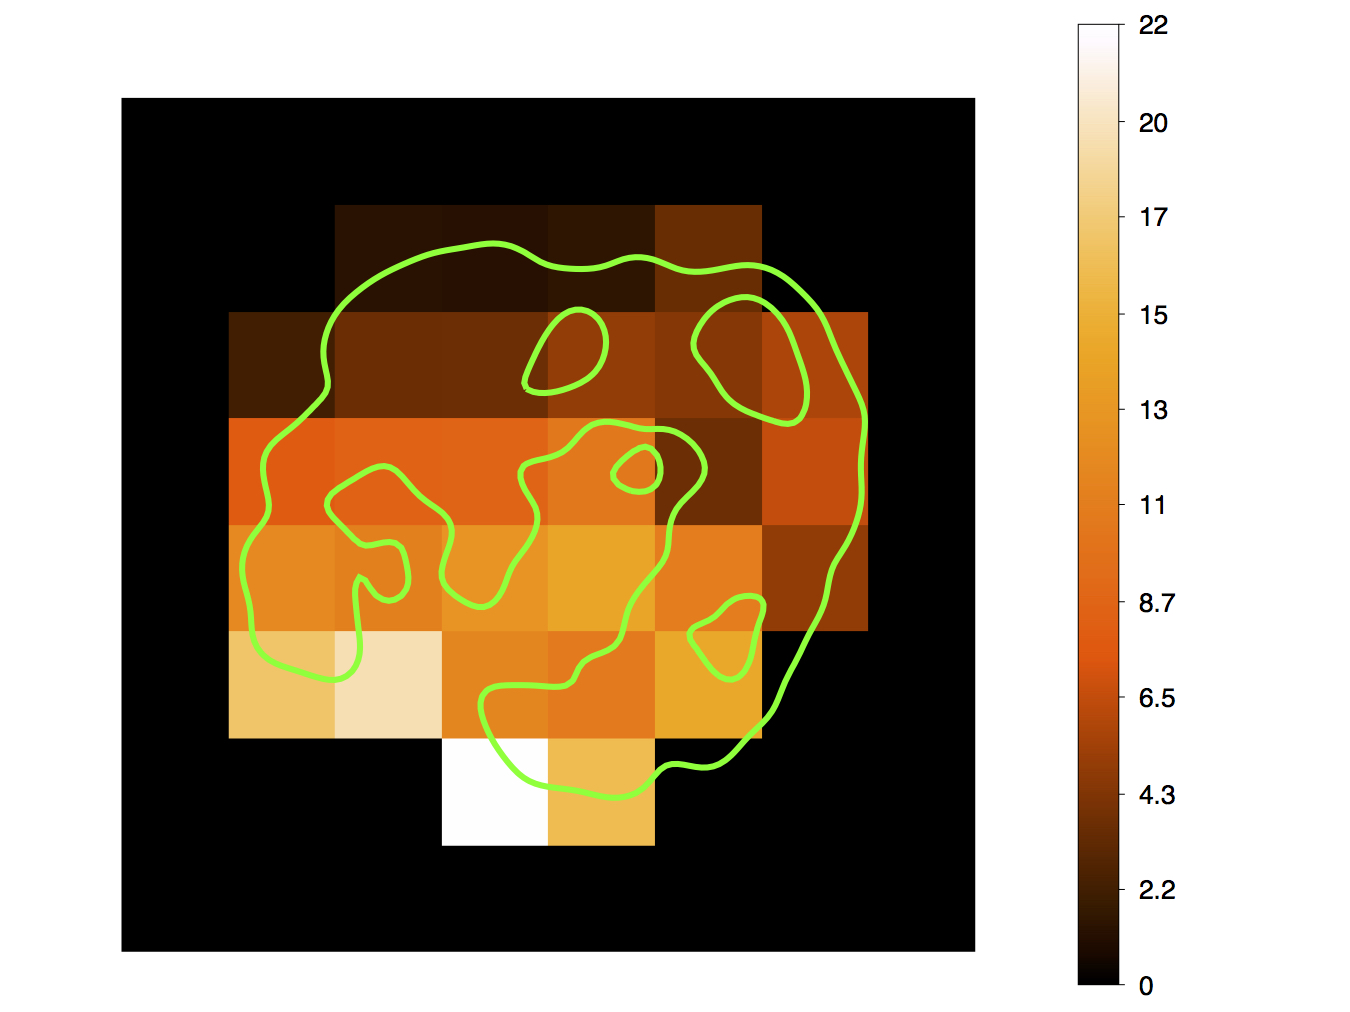
\includegraphics[width=.60\linewidth, height=0.27\textheight]{Wp_ratio_map}
	\caption{All regions colour coded according to their $R_{\mathrm{cool/SED}}$ values with the HESS $\gamma$-ray contours ($> 2$ TeV) overlaid in green.}
	\label{fig:wpratiocolourmap}
\end{figure}

We also draw on our results from the previous section where we obtained a proton injection energy for each region via 3 different methods (SED modeling, $10^{50}$ erg model and the cooling time model based on the HESS data). The injection energies obtained through the SED modeling and cooling time model were analysed further and a ratio of the two values, $R_{\mathrm{cool/SED}}$, for each region was calculated. This ratio is a measure of how consistent these two models are with each other and how successful the hadronic scenario is at explaining the $\gamma$-ray flux seen in each region. Figure \ref{fig:wpratiocolourmap} displays $R_{\mathrm{cool/SED}}$ for each region on a colour-scaled plot. The lower the value (and darker the region) the more successful our hadronic models were. We can compare these results with our results above to see if we get consistent predictions. 

The hadronic scenario was argued to be responsible for the $\gamma$-ray emission on the eastern, northern and southern sides of the SNR. From figure \ref{fig:wpratiocolourmap} we can see the success of the hadronic models in the northern and eastern regions as expected. The hadronic models appear to be inconsistent for the western and southern regions and towards the centre of the source. This is in agreement with our correlation study except for the case of regions 28 and 29. Both these regions contain very dense gas beyond the $\gamma$-ray shell. When modeling the SEDs for these regions we assume the CR protons interact with all of this gas, however because the shock front (and CR protons) have not yet reached this gas, this is not the case. The SED injection energy is inversely proportional to the gas density, hence lowering it to a density that corresponds to the actual target gas density will increase our SED injection energy. 

\subsection{Quantitative $\gamma$-ray and X-ray Flux Correlation Analysis}


\subsection{Quantitative ISM Gas Density and X-ray Flux Correlation Analysis}
We perform a correlation study between the ISM gas density and the \textit{Suzaku} X-ray flux, proceeding similarly as section \ref{sec:gasgamma}. The molecular gas density is calculated using only the Mopra $^{12}$ data set for this section. The \textit{Suzaku} data set is re-binned to ensure all data points are independent, since the data is smoothed with a Gaussian of radius $0.3^{\prime}$, we require a threshold pixel size of at least $0.6^{\prime} \times 0.6^{\prime} $. The Miriad function "imbin" only allows the re-binning, or averaging, to be done over whole numbers. So the smallest whole number that we can average over to obtain a pixel size larger than the threshold size is 3. The original pixel size is $16.6^{\prime \prime} \times 16.6^{\prime \prime}$, so the new pixel size becomes $0.83^{\prime} \times 0.83^{\prime}$. This provides us with a data set of 13 pixels by 13 pixels (169 pixels total) for each region. 
The Nanten telescope doesn't have the same resolution as the Mopra telescope, thus requiring us to re-grid the \textit{Suzaku} data set to fit the lower resolution Nanten data set. In such a case the resulting data sets would not be consistent with those obtained with the Mopra data set, losing any potential comparativeness. 


\begin{figure}[H]
	\begin{subfigure}{0.5\textwidth}
		\centering
		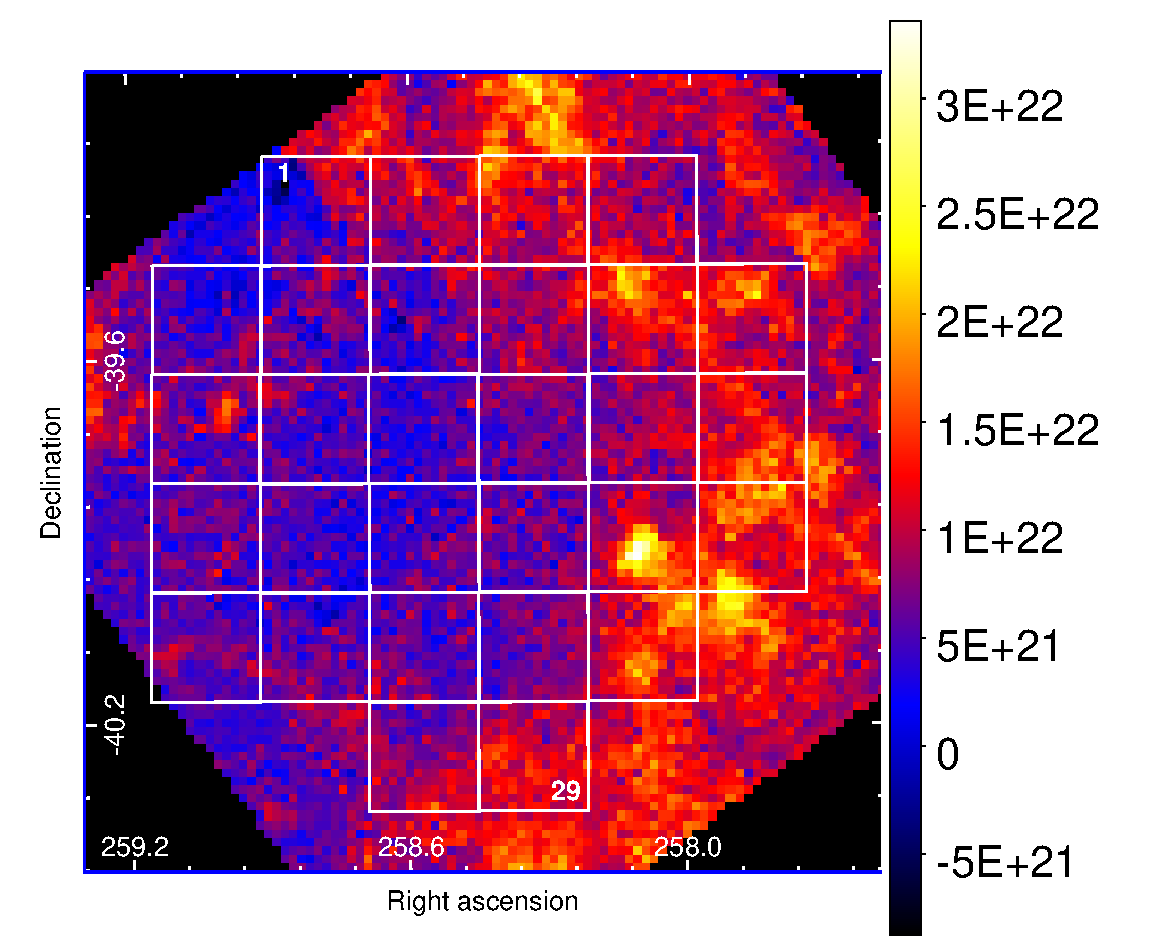
\includegraphics[width=1.0\linewidth, height=0.25\textheight]{Np_mopra_13pixels}
		\caption{}
		\label{fig:npmopra13pixels}
	\end{subfigure}
	\begin{subfigure}{0.5\textwidth}
		\centering
		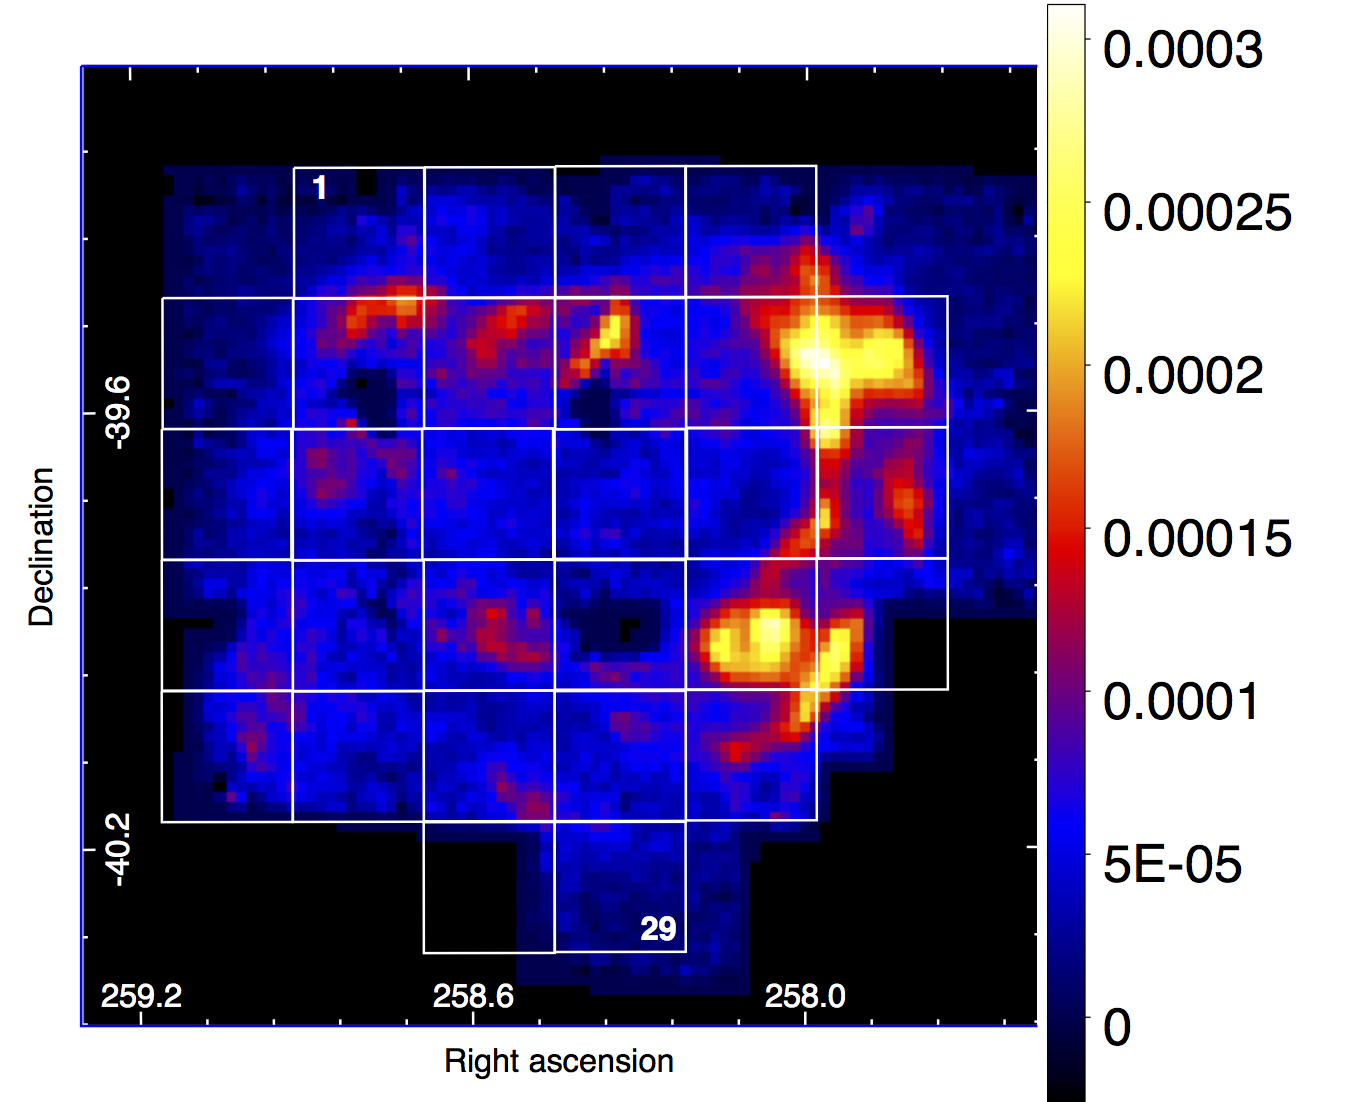
\includegraphics[width=1.0\linewidth, height=0.25\textheight]{suzaku_13pixelrebin}
		\caption{}
		\label{fig:suzaku13pixelrebin}
	\end{subfigure}
\end{figure}


\pagebreak


\newpage

\section{Diffusion}


\clearpage

\title{\LARGE \textbf{References}}
\bibliography{bibliography}
\newpage
\begin{appendices}
	\section{}
	\begin{figure}[H]
		\centering
		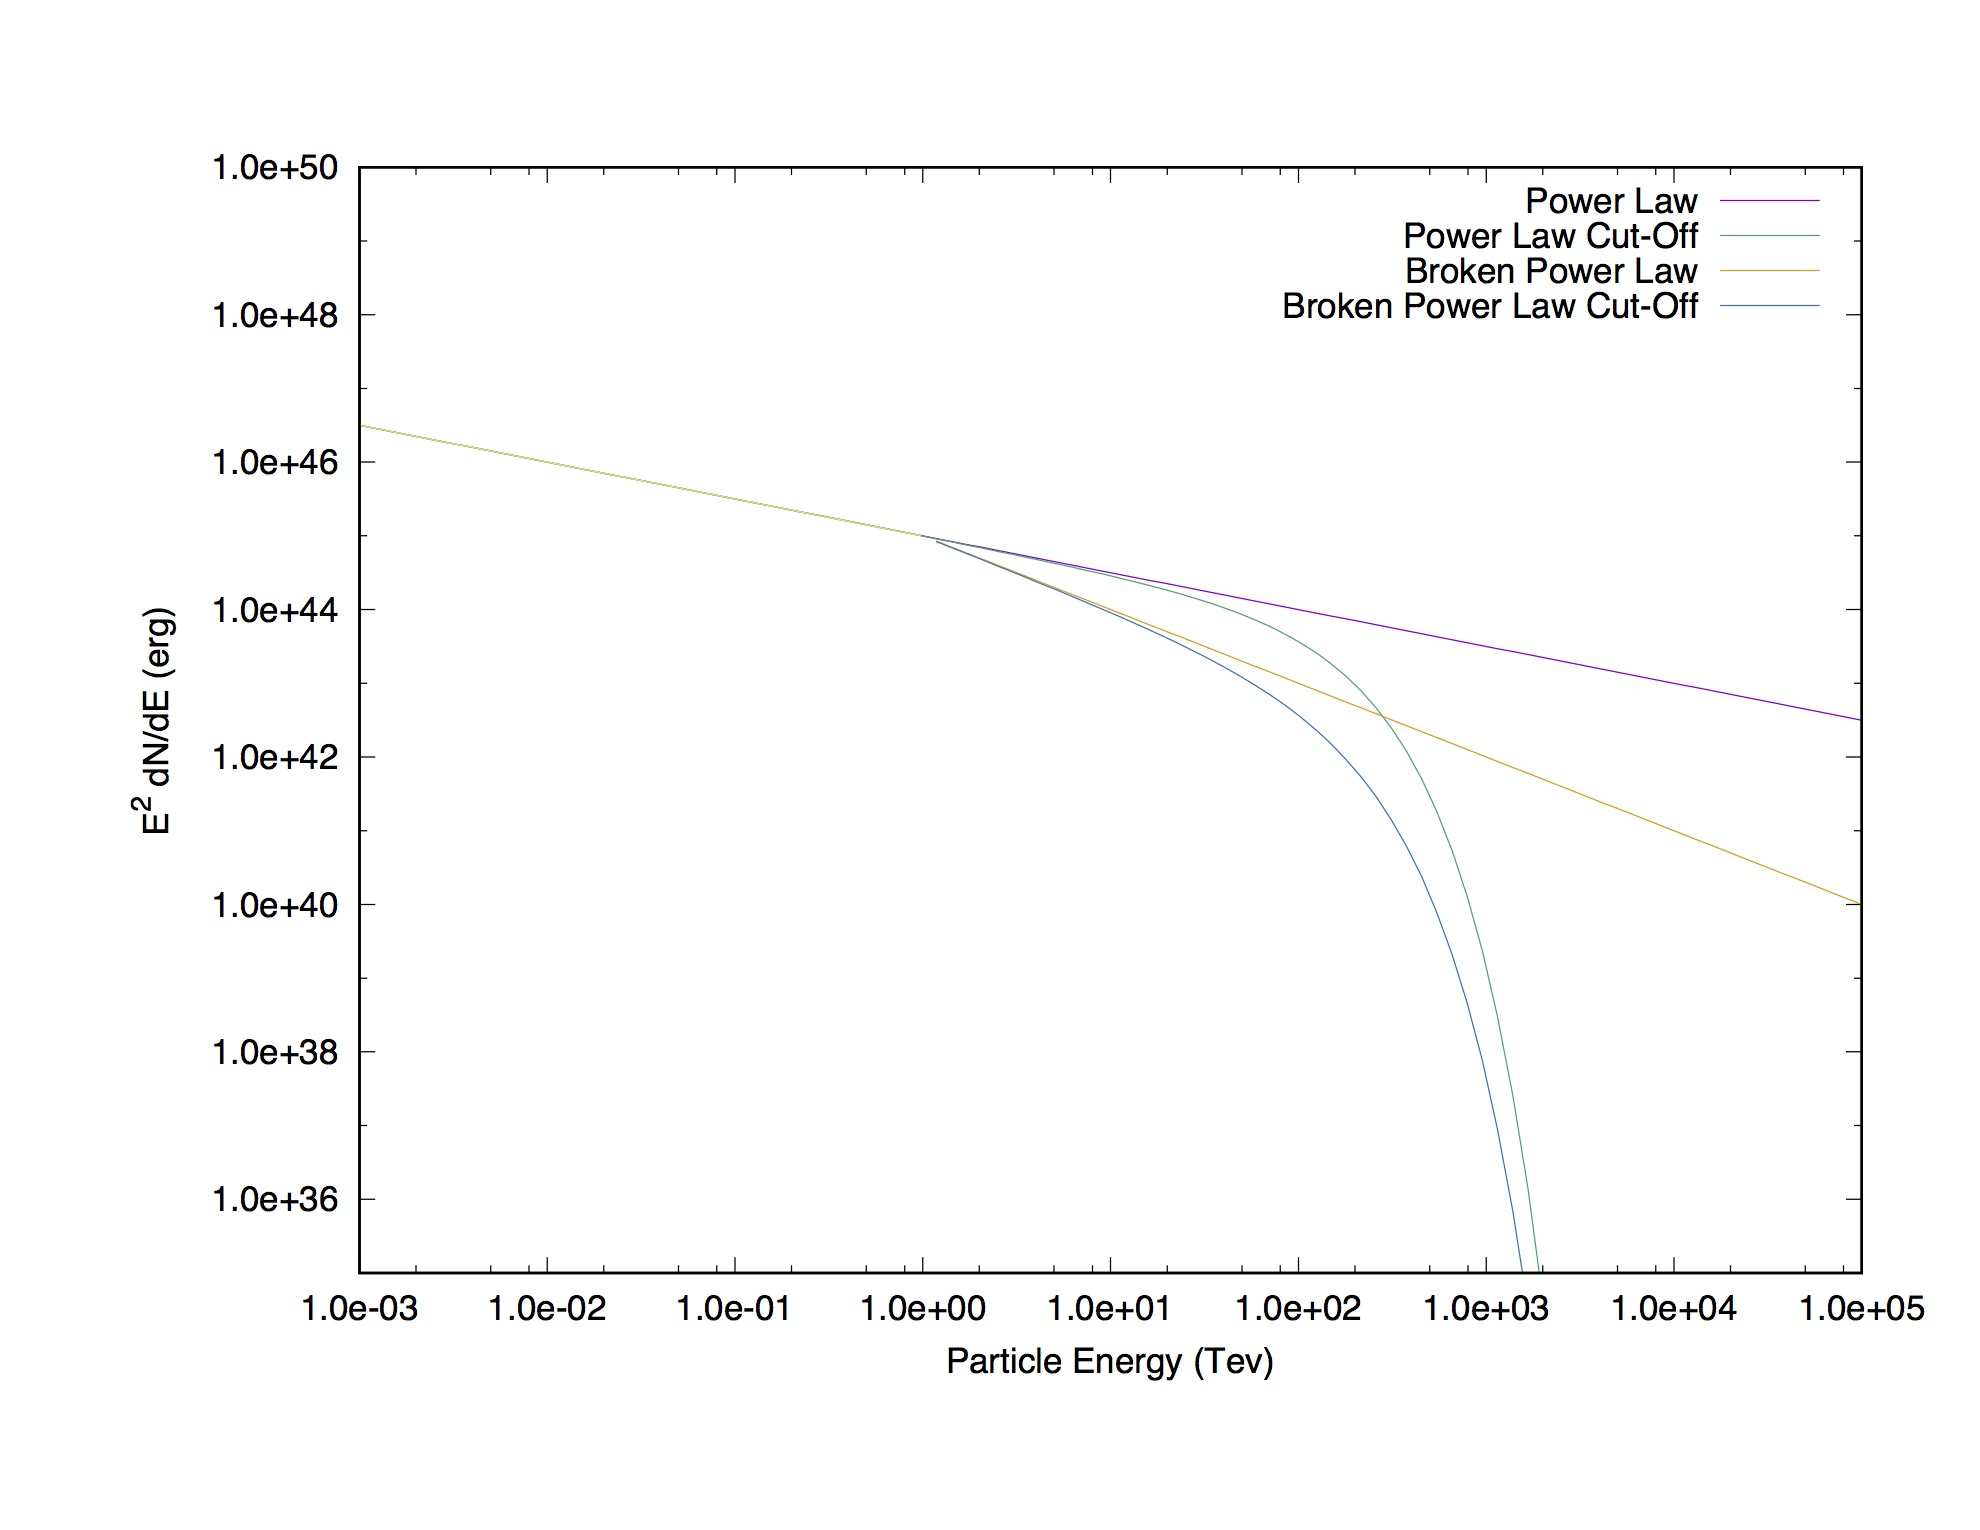
\includegraphics[width=0.55\linewidth, height=0.4\textheight, angle=-90]{powerlaws}
		\caption[]{Comparison of the various functional forms of the PL with a normalisation constant of $10^{45}$. The low energy spectral index $\alpha$ was taken to be 2.5 and the high energy spectral index $\beta$ was taken to be 3.0. $E_c$ and $E_b$ were also given typical values of 100 TeV and 1 TeV respectively.}
		\label{fig:powerlaws}
	\end{figure}
	\begin{figure}[H]
		\centering
		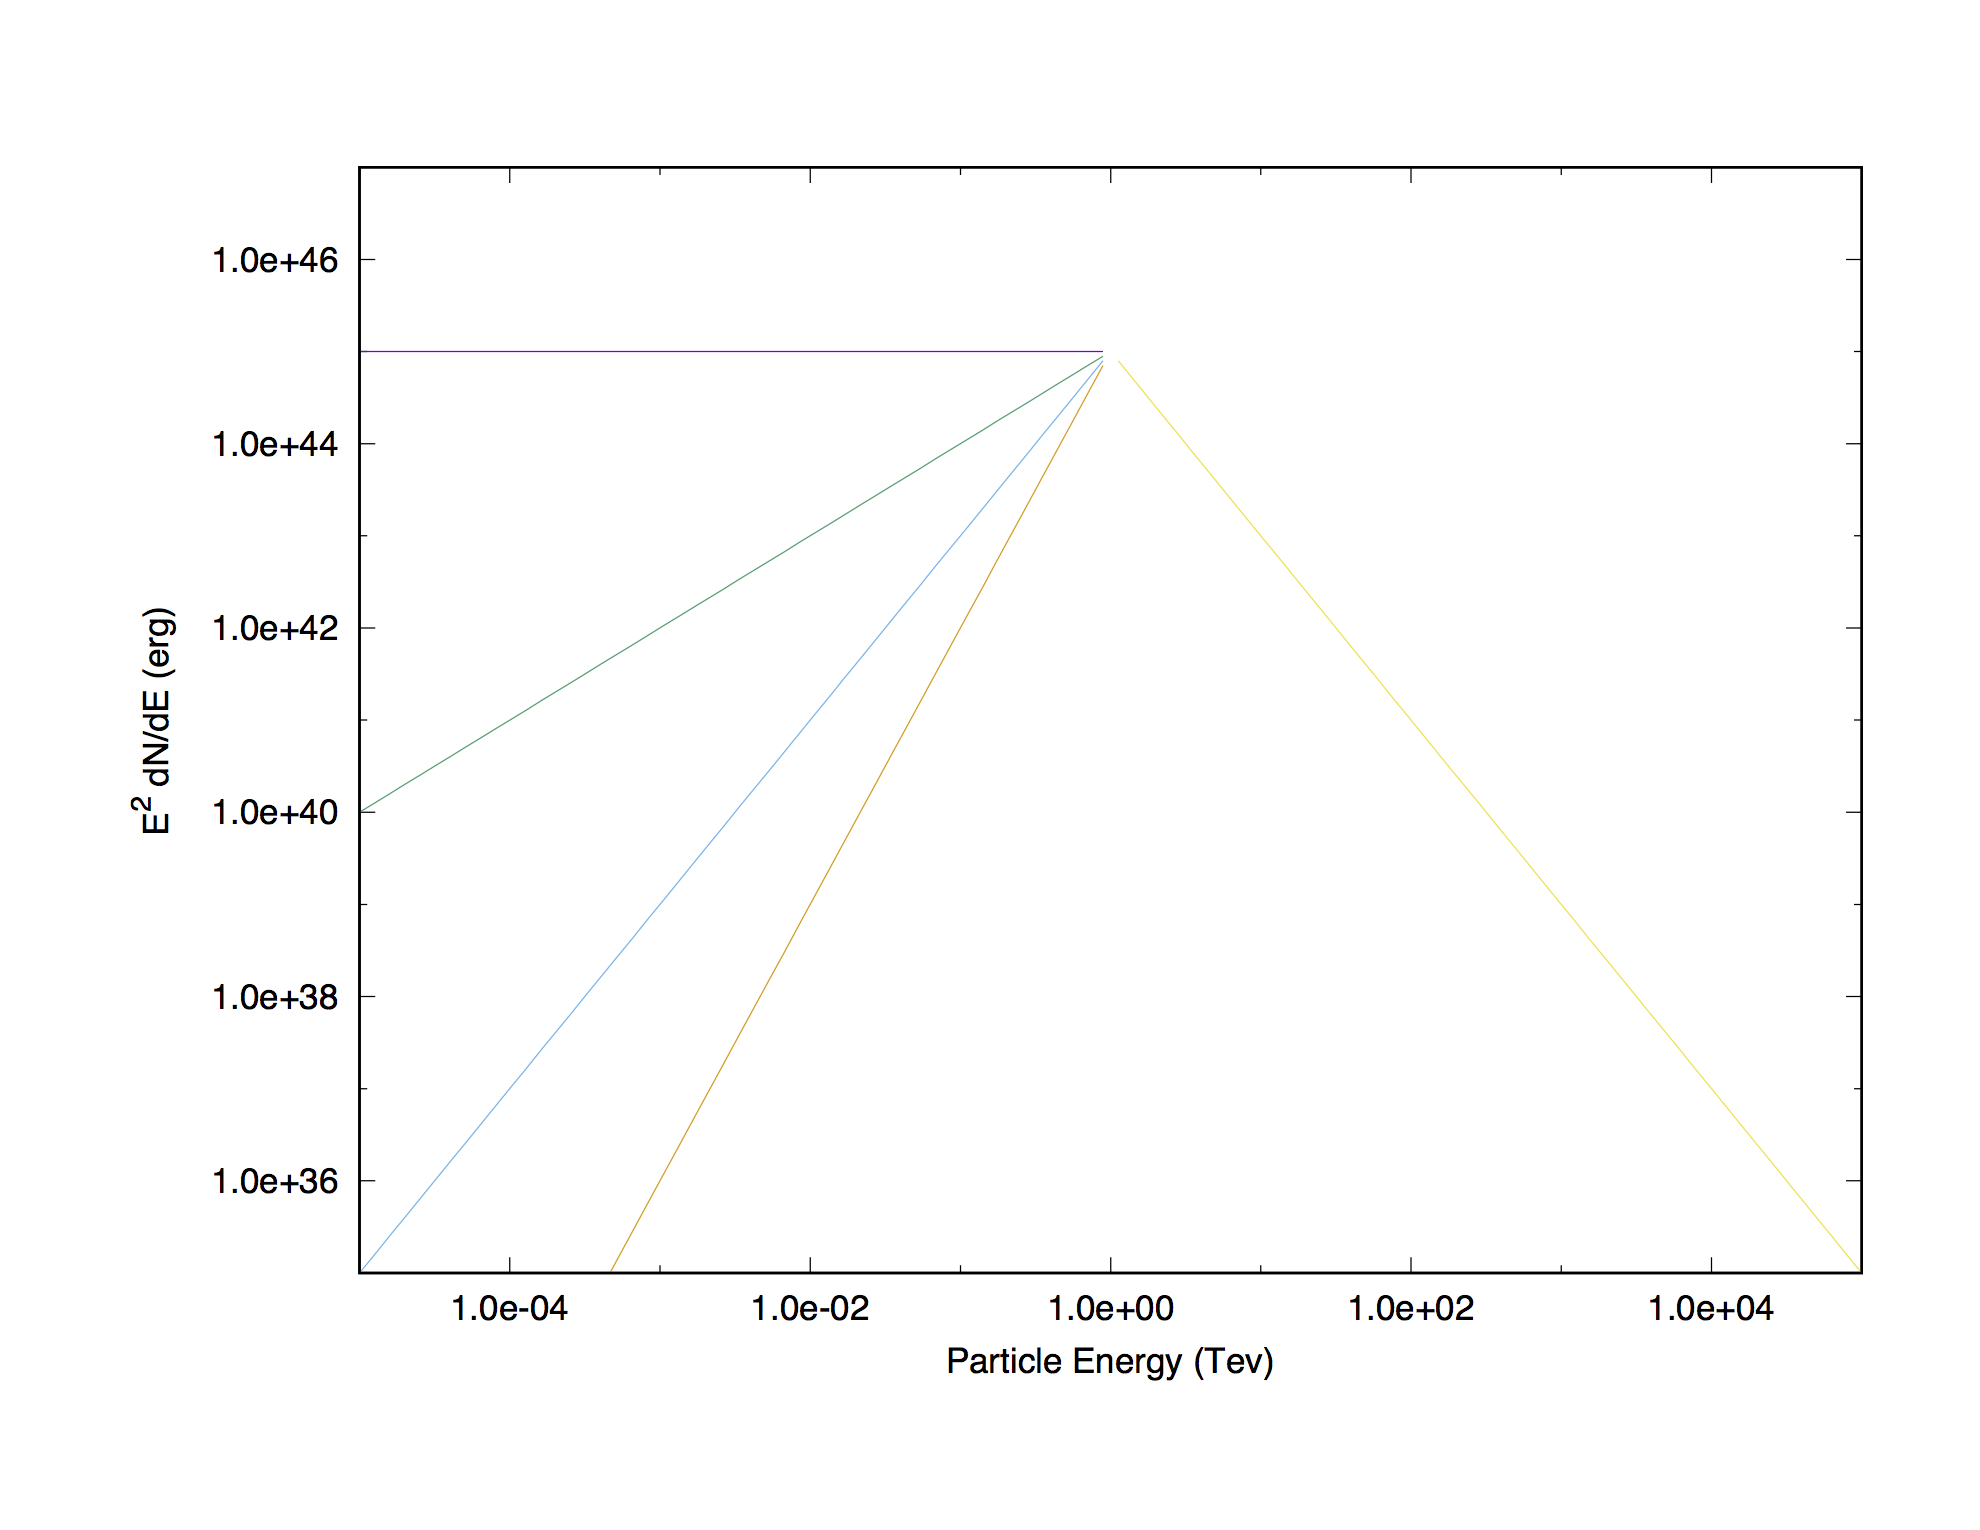
\includegraphics[width=0.55\linewidth, height=0.4\textheight, angle=-90]{powerlawsbroken}
		\caption{Broken power laws with variable low energy spectal indices $\alpha$ and fixed high energy spectrum index $\beta$ = 4. The purple, green, blue and orange lines correspond to a spectral index of $\alpha$ = 2.0, 1.0, 0.0 and -1.0 respectively.}
		\label{fig:powerlawsbroken}
	\end{figure}
	\begin{figure}[H]
		\centering
		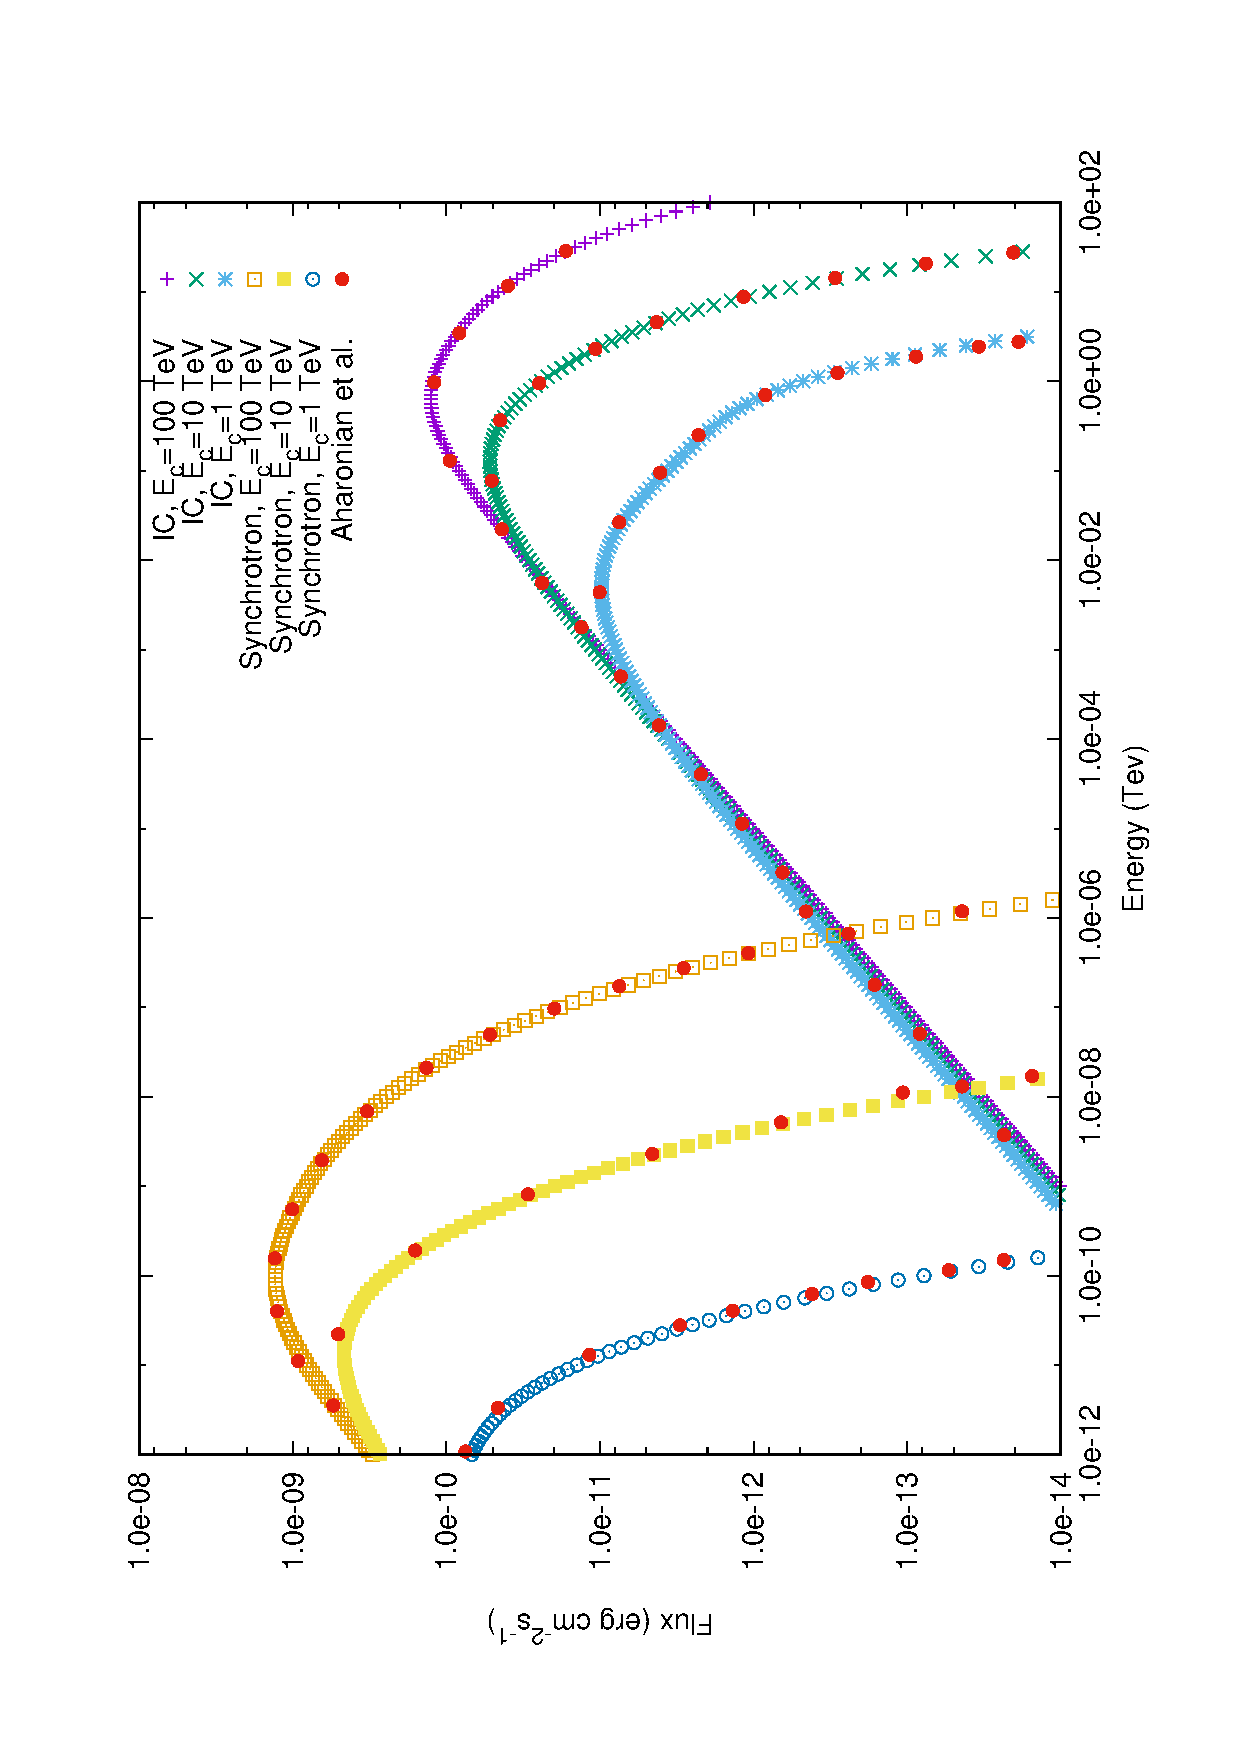
\includegraphics[width=0.52\linewidth, height=0.4\textheight, angle=-90]{kifunefig3b}
		\caption{An SED displaying the effect of altering the energy cut-off for an evolving electron distribution that follows a power law with an energy cut-off. The magnetic field has a value of $10 \mu$G, the injection energy is kept constant at $10^{37}$ erg s$^{-1}$ and the spectral index is chosen to be 2. The pulsar is taken to be 1 kpc away, 2 pc in size and $10^4$ years old. The IC contributions are based upon the photon fields of the 2.7 K CMB, diffuse galactic dust ($w_{FIR} = 0.05$ eV cm$^{-3}$ and T = 100 K) and optical radiation from stars ($w_{NIR} = 0.5$ eV cm$^{-3}$ and T = 5000 K). It can be seen that sedv2.c has successfully reproduced the work by Aharonian et al. (1997) (figure 3b).}
		\label{fig:kifunefig3b}
	\end{figure}
	 
	\begin{figure}[H]
		\centering
		\includegraphics[width=0.52\linewidth, height=0.4\textheight, angle=-90]{kifunefig3c}
		\caption{An SED displaying the effect of altering the age of the pulsar and keeping the cut-off energy constant at 100 TeV. The rest of the parameters are as above. We can also see once again that sedv2.c has correctly predicted the IC and synchrotron spectrum produced by Aharonian et al. (Figure 3c).}
		\label{fig:kifunefig3c}
	\end{figure}



 \cite{2012ApJ...746...82F} have already combined the NANTEN data with the HI data so we obtained a second proton column density map from their work. We simply re-grid this map to match the pixel size of the HESS map too. The derived final column density maps are illustrated in figure \ref{fig:moprahess9pixels} (bottom row). Note that the same factor of 51 was required to account for the re-griding process with the combined NANTEN-HI map.
 \begin{figure}
	\begin{subfigure}{0.5\textwidth}
		\centering
		\includegraphics[width=0.85\linewidth, height=0.22\textheight]{nanten_9pixels}
	\end{subfigure}
	\begin{subfigure}{0.5\textwidth}
		\centering
		\includegraphics[width=0.85\linewidth, height=0.22\textheight]{nanten_HI_9pixels}
	\end{subfigure}
	\caption{regridded Nanten map and re-gridded NANTEN + HI map}
\end{figure}

Figure \ref{fig:regionalgasgammacornanten} illustrates some plots with the gas density calculated with the NANTEN data.

\begin{figure}[H]
	\begin{subfigure}{0.5\textwidth}
		\centering
		\includegraphics[width=0.95\linewidth, height=0.27\textheight]{gamma_nHI_reg2}
		\label{fig:gnHIreg2}
	\end{subfigure}
	\begin{subfigure}{0.5\textwidth}
		\centering
		\includegraphics[width=0.9\linewidth, height=0.27\textheight]{gamma_nHI_reg3}
		\label{fig:gnHIreg3}
	\end{subfigure}
	\begin{subfigure}{0.5\textwidth}
		\centering
		\includegraphics[width=0.9\linewidth, height=0.27\textheight]{gamma_nHI_reg5}
		\label{fig:gnHIreg5}
	\end{subfigure}
	\begin{subfigure}{0.5\textwidth}
		\centering
		\includegraphics[width=0.9\linewidth, height=0.27\textheight]{gamma_nHI_reg12}
		\label{fig:gnHIreg12}
	\end{subfigure}
	\begin{subfigure}{0.5\textwidth}
		\centering
		\includegraphics[width=0.9\linewidth, height=0.27\textheight]{gamma_nHI_reg15}
		\label{fig:gnHIreg15}
	\end{subfigure}
	\begin{subfigure}{0.5\textwidth}
		\centering
		\includegraphics[width=0.9\linewidth, height=0.27\textheight]{gamma_nHI_reg21}
		\label{fig:gnHIreg21}
	\end{subfigure}
	\caption{Correlation plots between the ISM gas density and $\gamma$-ray flux using the NANTEN data for the molecular component of the gas density. The line of best fit for each data set is shown in black, while the grey area illustrates the confidence bands. Regions that display significant correlations are shown.}
	\label{fig:regionalgasgammacornanten}
\end{figure}

\begin{table}[H] 
	\centering
	\begin{tabular}{ccccccccc}
		Reg. && $\rho_\mathrm{M}$ & $p_\mathrm{M}$ & Significant$_\mathrm{M}$ && $\rho_\mathrm{N}$ & $p_\mathrm{N}$ & Significant$_\mathrm{N}$ \\
		\hline 
		1 && 0.52 & 0.150 & no && -0.06 & 0.877 & no \\
		\rowcolor{lightgray} 2 && -0.29 & 0.445 & no && -0.67 & 0.046 & yes \\
		\rowcolor{teal} 3 && -0.71 & 0.032 & yes && -0.74 & 0.023 & yes \\
		\rowcolor{lightgray} 4 && 0.80 & 0.009 & yes && 0.24 & 0.531 & no \\
		\rowcolor{lightgray} 5 && 0.09 & 0.812 & no && 0.88 & 0.002 & yes \\
		6 && -0.00 & 0.996 & no && 0.01 & 0.987 & no \\ 
		7 && 0.01 & 0.987 & no && -0.07 & 0.856 & no \\
		8 && 0.02 & 0.965 & no && 0.10 & 0.806 & no \\
		9 && 0.39 & 0.306 & no && 0.56 & 0.115 & no \\
		10 && 0.11 & 0.769 & no && 0.06 & 0.883 & no \\
		11 && -0.04 & 0.913 & no && 0.57 & 0.110 & no \\
		\rowcolor{lightgray} 12 && 0.54 & 0.135 & no && 0.77 & 0.015 & yes \\
		13 && -0.02 & 0.965 & no && -0.26 & 0.493 & no \\
		\rowcolor{lightgray} 14 && -0.74 & 0.022 & yes && 0.21 & 0.585 & no \\
		\rowcolor{lightgray} 15 && 0.34 & 0.365 & no && 0.75 & 0.019 & yes \\
		\rowcolor{lightgray} 16 && 0.80 & 0.009 & yes && 0.15 & 0.692 & no \\ 
		17 && -0.11 & 0.778 & no && 0.27 & 0.480 & no \\
		18 && 0.56 & 0.118 & no && 0.63 & 0.066 & no \\
		19 && 0.13 & 0.746 & no && -0.35 & 0.352 & no \\
		20 && 0.01 & 0.970 & no && 0.53 & 0.143 & no \\
		\rowcolor{lightgray} 21 && 0.49 & 0.182 & no && 0.73 & 0.025 & yes \\
		22 && 0.44 & 0.236 & no && 0.40 & 0.287 & no \\
		23 && -0.62 & 0.076 & no && -0.21 & 0.579 & no \\
		24 && -0.25 & 0.514 & no && -0.08 & 0.837 & no \\
		25 && 0.12 & 0.767 & no && -0.26 & 0.492 & no \\
		26 && -0.02 & 0.969 & no && 0.42 & 0.261 & no \\ 
		27 && 0.24 & 0.540 & no && 0.46 & 0.217 & no \\
		28 && 0.04 & 0.920 & no && -0.22 & 0.570 & no \\
		29 && -0.40 & 0.285 & no && -0.42 & 0.258 & no \\
		\hline 
	\end{tabular} 
	\caption{The calculated Pearson correlation coefficients and associated p-values for the gas density and the HESS $\gamma$-ray flux ($> 2$ TeV) data for each region and for both Mopra and NANTEN data sets. Grey shading indicates regions that have a significant p-value for either data set. Teal shading indicates regions that have a significant p-value for both data sets.}
	\label{tab:gasgammacor}
\end{table}

\end{appendices}
\end{document}